\documentclass[twoside]{book}

% Packages required by doxygen
\usepackage{fixltx2e}
\usepackage{calc}
\usepackage{doxygen}
\usepackage[export]{adjustbox} % also loads graphicx
\usepackage{graphicx}
\usepackage[utf8]{inputenc}
\usepackage{makeidx}
\usepackage{multicol}
\usepackage{multirow}
\PassOptionsToPackage{warn}{textcomp}
\usepackage{textcomp}
\usepackage[nointegrals]{wasysym}
\usepackage[table]{xcolor}

% Font selection
\usepackage[T1]{fontenc}
\usepackage[scaled=.90]{helvet}
\usepackage{courier}
\usepackage{amssymb}
\usepackage{sectsty}
\renewcommand{\familydefault}{\sfdefault}
\allsectionsfont{%
  \fontseries{bc}\selectfont%
  \color{darkgray}%
}
\renewcommand{\DoxyLabelFont}{%
  \fontseries{bc}\selectfont%
  \color{darkgray}%
}
\newcommand{\+}{\discretionary{\mbox{\scriptsize$\hookleftarrow$}}{}{}}

% Page & text layout
\usepackage{geometry}
\geometry{%
  a4paper,%
  top=2.5cm,%
  bottom=2.5cm,%
  left=2.5cm,%
  right=2.5cm%
}
\tolerance=750
\hfuzz=15pt
\hbadness=750
\setlength{\emergencystretch}{15pt}
\setlength{\parindent}{0cm}
\setlength{\parskip}{3ex plus 2ex minus 2ex}
\makeatletter
\renewcommand{\paragraph}{%
  \@startsection{paragraph}{4}{0ex}{-1.0ex}{1.0ex}{%
    \normalfont\normalsize\bfseries\SS@parafont%
  }%
}
\renewcommand{\subparagraph}{%
  \@startsection{subparagraph}{5}{0ex}{-1.0ex}{1.0ex}{%
    \normalfont\normalsize\bfseries\SS@subparafont%
  }%
}
\makeatother

% Headers & footers
\usepackage{fancyhdr}
\pagestyle{fancyplain}
\fancyhead[LE]{\fancyplain{}{\bfseries\thepage}}
\fancyhead[CE]{\fancyplain{}{}}
\fancyhead[RE]{\fancyplain{}{\bfseries\leftmark}}
\fancyhead[LO]{\fancyplain{}{\bfseries\rightmark}}
\fancyhead[CO]{\fancyplain{}{}}
\fancyhead[RO]{\fancyplain{}{\bfseries\thepage}}
\fancyfoot[LE]{\fancyplain{}{}}
\fancyfoot[CE]{\fancyplain{}{}}
\fancyfoot[RE]{\fancyplain{}{\bfseries\scriptsize Generated by Doxygen }}
\fancyfoot[LO]{\fancyplain{}{\bfseries\scriptsize Generated by Doxygen }}
\fancyfoot[CO]{\fancyplain{}{}}
\fancyfoot[RO]{\fancyplain{}{}}
\renewcommand{\footrulewidth}{0.4pt}
\renewcommand{\chaptermark}[1]{%
  \markboth{#1}{}%
}
\renewcommand{\sectionmark}[1]{%
  \markright{\thesection\ #1}%
}

% Indices & bibliography
\usepackage{natbib}
\usepackage[titles]{tocloft}
\setcounter{tocdepth}{3}
\setcounter{secnumdepth}{5}
\makeindex

% Hyperlinks (required, but should be loaded last)
\usepackage{ifpdf}
\ifpdf
  \usepackage[pdftex,pagebackref=true]{hyperref}
\else
  \usepackage[ps2pdf,pagebackref=true]{hyperref}
\fi
\hypersetup{%
  colorlinks=true,%
  linkcolor=blue,%
  citecolor=blue,%
  unicode%
}

% Custom commands
\newcommand{\clearemptydoublepage}{%
  \newpage{\pagestyle{empty}\cleardoublepage}%
}

\usepackage{caption}
\captionsetup{labelsep=space,justification=centering,font={bf},singlelinecheck=off,skip=4pt,position=top}

%===== C O N T E N T S =====

\begin{document}

% Titlepage & ToC
\hypersetup{pageanchor=false,
             bookmarksnumbered=true,
             pdfencoding=unicode
            }
\pagenumbering{alph}
\begin{titlepage}
\vspace*{7cm}
\begin{center}%
{\Large Goose Game \\[1ex]\large v0.\+3.\+1 }\\
\vspace*{1cm}
{\large Generated by Doxygen 1.8.13}\\
\end{center}
\end{titlepage}
\clearemptydoublepage
\pagenumbering{roman}
\tableofcontents
\clearemptydoublepage
\pagenumbering{arabic}
\hypersetup{pageanchor=true}

%--- Begin generated contents ---
\chapter{Data Structure Index}
\section{Data Structures}
Here are the data structures with brief descriptions\+:\begin{DoxyCompactList}
\item\contentsline{section}{\hyperlink{struct__Cmd}{\+\_\+\+Cmd} \\*Command data structure }{\pageref{struct__Cmd}}{}
\item\contentsline{section}{\hyperlink{struct__Die}{\+\_\+\+Die} \\*The die structure }{\pageref{struct__Die}}{}
\item\contentsline{section}{\hyperlink{struct__G__engine}{\+\_\+\+G\+\_\+engine} \\*Main graphic engine structure }{\pageref{struct__G__engine}}{}
\item\contentsline{section}{\hyperlink{struct__Game}{\+\_\+\+Game} }{\pageref{struct__Game}}{}
\item\contentsline{section}{\hyperlink{struct__Inventory}{\+\_\+\+Inventory} }{\pageref{struct__Inventory}}{}
\item\contentsline{section}{\hyperlink{struct__Object}{\+\_\+\+Object} \\*Main object structure }{\pageref{struct__Object}}{}
\item\contentsline{section}{\hyperlink{struct__Player}{\+\_\+\+Player} \\*Player\textquotesingle{}s structure }{\pageref{struct__Player}}{}
\item\contentsline{section}{\hyperlink{struct__Set}{\+\_\+\+Set} }{\pageref{struct__Set}}{}
\item\contentsline{section}{\hyperlink{struct__Space}{\+\_\+\+Space} }{\pageref{struct__Space}}{}
\item\contentsline{section}{\hyperlink{struct__Ui}{\+\_\+\+Ui} \\*Main UI structure }{\pageref{struct__Ui}}{}
\item\contentsline{section}{\hyperlink{struct__Ui__box}{\+\_\+\+Ui\+\_\+box} \\*Main box structure }{\pageref{struct__Ui__box}}{}
\item\contentsline{section}{\hyperlink{struct__Ui__pix}{\+\_\+\+Ui\+\_\+pix} \\*Basic pixel structure }{\pageref{struct__Ui__pix}}{}
\item\contentsline{section}{\hyperlink{struct__Ui__screen}{\+\_\+\+Ui\+\_\+screen} \\*Main UI screen structure }{\pageref{struct__Ui__screen}}{}
\end{DoxyCompactList}

\chapter{File Index}
\section{File List}
Here is a list of all documented files with brief descriptions\+:\begin{DoxyCompactList}
\item\contentsline{section}{inc/\hyperlink{cmd_8h}{cmd.\+h} \\*Command interpreter }{\pageref{cmd_8h}}{}
\item\contentsline{section}{inc/\hyperlink{die_8h}{die.\+h} \\*Die\textquotesingle{}s module header }{\pageref{die_8h}}{}
\item\contentsline{section}{inc/\hyperlink{g__engine_8h}{g\+\_\+engine.\+h} \\*Main graphic engine }{\pageref{g__engine_8h}}{}
\item\contentsline{section}{inc/\hyperlink{game_8h}{game.\+h} \\*It defines the game interface }{\pageref{game_8h}}{}
\item\contentsline{section}{inc/{\bfseries game\+\_\+rules.\+h} }{\pageref{game__rules_8h}}{}
\item\contentsline{section}{inc/\hyperlink{inventory_8h}{inventory.\+h} \\*Inventory manager }{\pageref{inventory_8h}}{}
\item\contentsline{section}{inc/\hyperlink{link_8h}{link.\+h} \\*Link functions }{\pageref{link_8h}}{}
\item\contentsline{section}{inc/\hyperlink{log_8h}{log.\+h} \\*Logger }{\pageref{log_8h}}{}
\item\contentsline{section}{inc/\hyperlink{manager_8h}{manager.\+h} \\*Defines a game reader }{\pageref{manager_8h}}{}
\item\contentsline{section}{inc/\hyperlink{object_8h}{object.\+h} \\*Object manager }{\pageref{object_8h}}{}
\item\contentsline{section}{inc/\hyperlink{player_8h}{player.\+h} \\*Player header }{\pageref{player_8h}}{}
\item\contentsline{section}{inc/\hyperlink{set_8h}{set.\+h} \\*It defines the set interface }{\pageref{set_8h}}{}
\item\contentsline{section}{inc/\hyperlink{space_8h}{space.\+h} \\*Space module }{\pageref{space_8h}}{}
\item\contentsline{section}{inc/{\bfseries str.\+h} }{\pageref{str_8h}}{}
\item\contentsline{section}{inc/{\bfseries test.\+h} }{\pageref{test_8h}}{}
\item\contentsline{section}{inc/\hyperlink{types_8h}{types.\+h} \\*It defines types of data }{\pageref{types_8h}}{}
\item\contentsline{section}{inc/\hyperlink{ui_8h}{ui.\+h} \\*User interface based on chars }{\pageref{ui_8h}}{}
\item\contentsline{section}{src/\hyperlink{cmd_8c}{cmd.\+c} \\*Command source code }{\pageref{cmd_8c}}{}
\item\contentsline{section}{src/\hyperlink{die_8c}{die.\+c} \\*Die\textquotesingle{}s module dynamic }{\pageref{die_8c}}{}
\item\contentsline{section}{src/\hyperlink{g__engine_8c}{g\+\_\+engine.\+c} \\*Graphic engine source code }{\pageref{g__engine_8c}}{}
\item\contentsline{section}{src/\hyperlink{game__loop_8c}{game\+\_\+loop.\+c} \\*Main game loop }{\pageref{game__loop_8c}}{}
\item\contentsline{section}{src/\hyperlink{inventory_8c}{inventory.\+c} \\*Code implementation of the inventory manager }{\pageref{inventory_8c}}{}
\item\contentsline{section}{src/\hyperlink{inventory__tb_8c}{inventory\+\_\+tb.\+c} \\*Main for test the inventory }{\pageref{inventory__tb_8c}}{}
\item\contentsline{section}{src/\hyperlink{link_8c}{link.\+c} \\*Link functions }{\pageref{link_8c}}{}
\item\contentsline{section}{src/\hyperlink{link__tb_8c}{link\+\_\+tb.\+c} \\*Main for test the link }{\pageref{link__tb_8c}}{}
\item\contentsline{section}{src/\hyperlink{log_8c}{log.\+c} \\*Logger }{\pageref{log_8c}}{}
\item\contentsline{section}{src/\hyperlink{manager_8c}{manager.\+c} \\*Main game reader }{\pageref{manager_8c}}{}
\item\contentsline{section}{src/\hyperlink{object_8c}{object.\+c} \\*Manages the game objects }{\pageref{object_8c}}{}
\item\contentsline{section}{src/\hyperlink{object__tb_8c}{object\+\_\+tb.\+c} \\*Object testbench evaluates each object function for each case }{\pageref{object__tb_8c}}{}
\item\contentsline{section}{src/\hyperlink{player_8c}{player.\+c} \\*Main player manager }{\pageref{player_8c}}{}
\item\contentsline{section}{src/\hyperlink{space_8c}{space.\+c} }{\pageref{space_8c}}{}
\item\contentsline{section}{src/\hyperlink{ui_8c}{ui.\+c} \\*Ui source code }{\pageref{ui_8c}}{}
\end{DoxyCompactList}

\chapter{Data Structure Documentation}
\hypertarget{struct__Cmd}{}\section{\+\_\+\+Cmd Struct Reference}
\label{struct__Cmd}\index{\+\_\+\+Cmd@{\+\_\+\+Cmd}}


Command data structure.  


\subsection*{Data Fields}
\begin{DoxyCompactItemize}
\item 
\mbox{\Hypertarget{struct__Cmd_a106b2045967078710623e3a5f401dde2}\label{struct__Cmd_a106b2045967078710623e3a5f401dde2}} 
\hyperlink{cmd_8h_a2933336e1f8003400f3b050402f0f5f3}{Cid} \hyperlink{struct__Cmd_a106b2045967078710623e3a5f401dde2}{id}
\begin{DoxyCompactList}\small\item\em Command identification. \end{DoxyCompactList}\item 
\mbox{\Hypertarget{struct__Cmd_af56ffa5c8c8f19251b15dc02a7eb352d}\label{struct__Cmd_af56ffa5c8c8f19251b15dc02a7eb352d}} 
int \hyperlink{struct__Cmd_af56ffa5c8c8f19251b15dc02a7eb352d}{argc}
\begin{DoxyCompactList}\small\item\em Number of arguments. \end{DoxyCompactList}\item 
\mbox{\Hypertarget{struct__Cmd_aaaa6f539ab5219743163ecb74138fe7a}\label{struct__Cmd_aaaa6f539ab5219743163ecb74138fe7a}} 
char $\ast$ \hyperlink{struct__Cmd_aaaa6f539ab5219743163ecb74138fe7a}{argv} \mbox{[}\hyperlink{cmd_8h_a64bf1979142baf43271722ff7b14c17d}{M\+A\+X\+\_\+\+C\+M\+D\+\_\+\+A\+R\+GC}\mbox{]}
\begin{DoxyCompactList}\small\item\em Value of the arguments. \end{DoxyCompactList}\item 
\mbox{\Hypertarget{struct__Cmd_adb97870a775bf9f9075d44420cb82439}\label{struct__Cmd_adb97870a775bf9f9075d44420cb82439}} 
char \hyperlink{struct__Cmd_adb97870a775bf9f9075d44420cb82439}{b\+\_\+name} \mbox{[}\hyperlink{cmd_8h_a1eb73c104b484cf18752169509cebfe2}{M\+A\+X\+\_\+\+C\+M\+D\+\_\+\+L\+EN}\mbox{]}
\begin{DoxyCompactList}\small\item\em Base name. \end{DoxyCompactList}\item 
\mbox{\Hypertarget{struct__Cmd_ac7a8c09e258cb2b2f63d179943616d08}\label{struct__Cmd_ac7a8c09e258cb2b2f63d179943616d08}} 
char \hyperlink{struct__Cmd_ac7a8c09e258cb2b2f63d179943616d08}{s\+\_\+name} \mbox{[}\hyperlink{cmd_8h_a1eb73c104b484cf18752169509cebfe2}{M\+A\+X\+\_\+\+C\+M\+D\+\_\+\+L\+EN}\mbox{]}
\begin{DoxyCompactList}\small\item\em Short name. \end{DoxyCompactList}\item 
\mbox{\Hypertarget{struct__Cmd_a3d023ded28ab2b9ec8daae3ebf1a3759}\label{struct__Cmd_a3d023ded28ab2b9ec8daae3ebf1a3759}} 
char \hyperlink{struct__Cmd_a3d023ded28ab2b9ec8daae3ebf1a3759}{input} \mbox{[}\hyperlink{cmd_8h_a536329c6bdf286710c20c6dd9a0750cc}{M\+A\+X\+\_\+\+C\+M\+D\+\_\+\+IN}\mbox{]}
\begin{DoxyCompactList}\small\item\em Cmd input. \end{DoxyCompactList}\item 
\mbox{\Hypertarget{struct__Cmd_a143c62700ed611e1ff0d70611c76fa55}\label{struct__Cmd_a143c62700ed611e1ff0d70611c76fa55}} 
char \hyperlink{struct__Cmd_a143c62700ed611e1ff0d70611c76fa55}{answer} \mbox{[}\hyperlink{cmd_8h_ab972c58772002197942552cc47b6b5cd}{M\+A\+X\+\_\+\+C\+M\+D\+\_\+\+A\+NS}\mbox{]}
\begin{DoxyCompactList}\small\item\em Command answer. \end{DoxyCompactList}\item 
\mbox{\Hypertarget{struct__Cmd_a4f3acf8cfdc67548121c1989765cbbcf}\label{struct__Cmd_a4f3acf8cfdc67548121c1989765cbbcf}} 
int \hyperlink{struct__Cmd_a4f3acf8cfdc67548121c1989765cbbcf}{errc}
\begin{DoxyCompactList}\small\item\em Error code. \end{DoxyCompactList}\item 
\mbox{\Hypertarget{struct__Cmd_abfca5a0889206135702ed3e398079bad}\label{struct__Cmd_abfca5a0889206135702ed3e398079bad}} 
\hyperlink{cmd_8h_a78d7a8bd781b5514e6dd7e1253bb1907}{cmd\+\_\+fn} \hyperlink{struct__Cmd_abfca5a0889206135702ed3e398079bad}{fn}
\begin{DoxyCompactList}\small\item\em Callback function. \end{DoxyCompactList}\end{DoxyCompactItemize}


\subsection{Detailed Description}
Command data structure. 

The documentation for this struct was generated from the following file\+:\begin{DoxyCompactItemize}
\item 
src/cmd.\+c\end{DoxyCompactItemize}

\hypertarget{struct__Die}{}\section{\+\_\+\+Die Struct Reference}
\label{struct__Die}\index{\+\_\+\+Die@{\+\_\+\+Die}}


Die structure which contains information about Die.  


\subsection*{Data Fields}
\begin{DoxyCompactItemize}
\item 
\mbox{\Hypertarget{struct__Die_a0887af562dda760409957f13619d36f1}\label{struct__Die_a0887af562dda760409957f13619d36f1}} 
Id \hyperlink{struct__Die_a0887af562dda760409957f13619d36f1}{id}
\begin{DoxyCompactList}\small\item\em Die\textquotesingle{}s id. \end{DoxyCompactList}\item 
\mbox{\Hypertarget{struct__Die_abf73744a544920c64d79d84d964be62d}\label{struct__Die_abf73744a544920c64d79d84d964be62d}} 
int \hyperlink{struct__Die_abf73744a544920c64d79d84d964be62d}{last\+\_\+n}
\begin{DoxyCompactList}\small\item\em Die\textquotesingle{}s last number rolled. \end{DoxyCompactList}\end{DoxyCompactItemize}


\subsection{Detailed Description}
Die structure which contains information about Die. 

The documentation for this struct was generated from the following file\+:\begin{DoxyCompactItemize}
\item 
src/\hyperlink{die_8c}{die.\+c}\end{DoxyCompactItemize}

\hypertarget{struct__G__engine}{}\section{\+\_\+\+G\+\_\+engine Struct Reference}
\label{struct__G__engine}\index{\+\_\+\+G\+\_\+engine@{\+\_\+\+G\+\_\+engine}}


Main graphic engine structure.  




Collaboration diagram for \+\_\+\+G\+\_\+engine\+:
\nopagebreak
\begin{figure}[H]
\begin{center}
\leavevmode
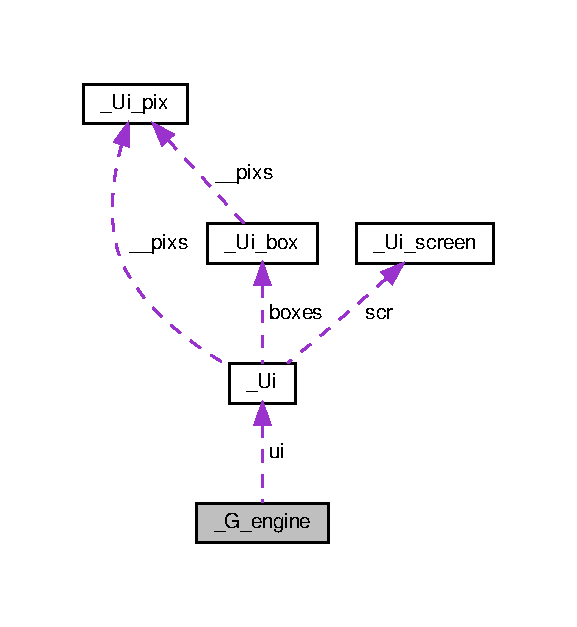
\includegraphics[width=277pt]{struct__G__engine__coll__graph}
\end{center}
\end{figure}
\subsection*{Data Fields}
\begin{DoxyCompactItemize}
\item 
\mbox{\Hypertarget{struct__G__engine_a56b776923e2d67db123587e106132365}\label{struct__G__engine_a56b776923e2d67db123587e106132365}} 
\hyperlink{struct__Ui}{Ui} $\ast$ \hyperlink{struct__G__engine_a56b776923e2d67db123587e106132365}{game\+\_\+ui}
\begin{DoxyCompactList}\small\item\em Game interface. \end{DoxyCompactList}\item 
\mbox{\Hypertarget{struct__G__engine_a76c426bc9bdd8031c0961abd5530e9c3}\label{struct__G__engine_a76c426bc9bdd8031c0961abd5530e9c3}} 
\hyperlink{struct__Ui}{Ui} $\ast$ \hyperlink{struct__G__engine_a76c426bc9bdd8031c0961abd5530e9c3}{help\+\_\+ui}
\begin{DoxyCompactList}\small\item\em Help interface. \end{DoxyCompactList}\end{DoxyCompactItemize}


\subsection{Detailed Description}
Main graphic engine structure. 

The documentation for this struct was generated from the following file\+:\begin{DoxyCompactItemize}
\item 
src/\hyperlink{g__engine_8c}{g\+\_\+engine.\+c}\end{DoxyCompactItemize}

\hypertarget{struct__Game}{}\section{\+\_\+\+Game Struct Reference}
\label{struct__Game}\index{\+\_\+\+Game@{\+\_\+\+Game}}


Game structure.  




Collaboration diagram for \+\_\+\+Game\+:
\nopagebreak
\begin{figure}[H]
\begin{center}
\leavevmode
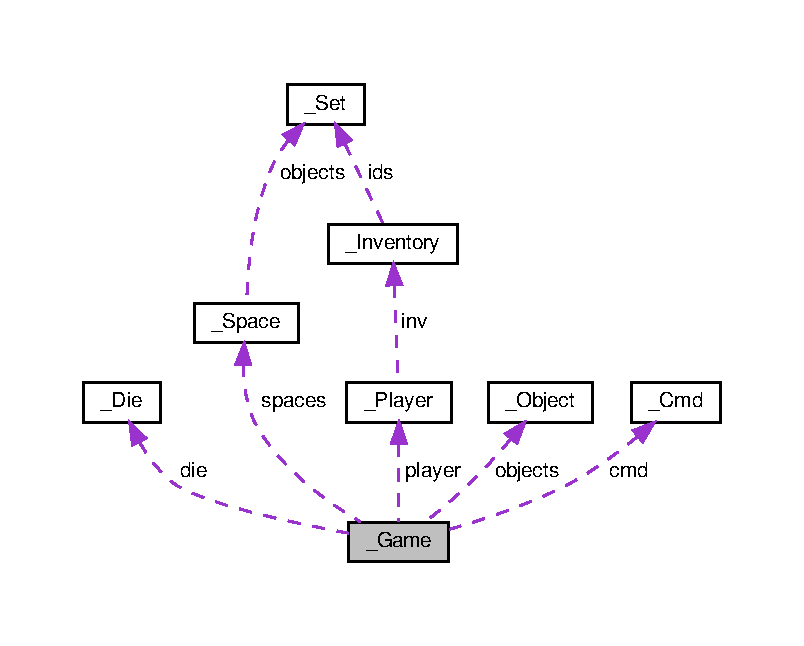
\includegraphics[width=350pt]{struct__Game__coll__graph}
\end{center}
\end{figure}
\subsection*{Data Fields}
\begin{DoxyCompactItemize}
\item 
\mbox{\Hypertarget{struct__Game_a31406605782d71ec00c4bf258ea76267}\label{struct__Game_a31406605782d71ec00c4bf258ea76267}} 
\hyperlink{struct__Player}{Player} $\ast$ \hyperlink{struct__Game_a31406605782d71ec00c4bf258ea76267}{player}
\begin{DoxyCompactList}\small\item\em players in game \end{DoxyCompactList}\item 
\mbox{\Hypertarget{struct__Game_a0d6009b5dcb080489c192a9198fa7d46}\label{struct__Game_a0d6009b5dcb080489c192a9198fa7d46}} 
\hyperlink{struct__Die}{Die} $\ast$ \hyperlink{struct__Game_a0d6009b5dcb080489c192a9198fa7d46}{die}
\begin{DoxyCompactList}\small\item\em game\textquotesingle{}s die \end{DoxyCompactList}\item 
\mbox{\Hypertarget{struct__Game_ad45bf5645a26e546d0060a2e61f9cf81}\label{struct__Game_ad45bf5645a26e546d0060a2e61f9cf81}} 
\hyperlink{object_8h_a7f8bbcda919b65ce67f92fba08e0212f}{Object} $\ast$ \hyperlink{struct__Game_ad45bf5645a26e546d0060a2e61f9cf81}{objects} \mbox{[}\hyperlink{object_8h_acdc7844fbd4d45737d4aa56834d37829}{M\+A\+X\+\_\+\+O\+B\+J\+E\+C\+TS}\mbox{]}
\begin{DoxyCompactList}\small\item\em Objects in game. \end{DoxyCompactList}\item 
\mbox{\Hypertarget{struct__Game_ab4180417d9148f8abb2233ca6c4ecfe5}\label{struct__Game_ab4180417d9148f8abb2233ca6c4ecfe5}} 
\hyperlink{space_8h_a67533ffc2b70463baecc38fb0629bbfc}{Space} $\ast$ \hyperlink{struct__Game_ab4180417d9148f8abb2233ca6c4ecfe5}{spaces} \mbox{[}\hyperlink{space_8h_a5f54fd55f983a2e33ce076cd9f587e82}{M\+A\+X\+\_\+\+S\+P\+A\+C\+ES}+1\mbox{]}
\begin{DoxyCompactList}\small\item\em Spaces in game. \end{DoxyCompactList}\item 
\mbox{\Hypertarget{struct__Game_ac98c89af82c9ffde3f17e7f4929bb97c}\label{struct__Game_ac98c89af82c9ffde3f17e7f4929bb97c}} 
\hyperlink{struct__Cmd}{Cmd} $\ast$ \hyperlink{struct__Game_ac98c89af82c9ffde3f17e7f4929bb97c}{cmd}
\begin{DoxyCompactList}\small\item\em Game commands. \end{DoxyCompactList}\item 
\mbox{\Hypertarget{struct__Game_a2b766f0814f66dcf437600a9c526142e}\label{struct__Game_a2b766f0814f66dcf437600a9c526142e}} 
\hyperlink{struct__Link}{Link} $\ast$ \hyperlink{struct__Game_a2b766f0814f66dcf437600a9c526142e}{links} \mbox{[}M\+A\+X\+\_\+\+L\+I\+N\+KS\mbox{]}
\begin{DoxyCompactList}\small\item\em Links in game. \end{DoxyCompactList}\end{DoxyCompactItemize}


\subsection{Detailed Description}
Game structure. 

The documentation for this struct was generated from the following file\+:\begin{DoxyCompactItemize}
\item 
src/game.\+c\end{DoxyCompactItemize}

\hypertarget{struct__Inventory}{}\section{\+\_\+\+Inventory Struct Reference}
\label{struct__Inventory}\index{\+\_\+\+Inventory@{\+\_\+\+Inventory}}


Collaboration diagram for \+\_\+\+Inventory\+:\nopagebreak
\begin{figure}[H]
\begin{center}
\leavevmode
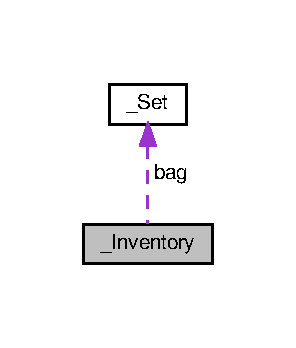
\includegraphics[width=142pt]{struct__Inventory__coll__graph}
\end{center}
\end{figure}
\subsection*{Data Fields}
\begin{DoxyCompactItemize}
\item 
\mbox{\Hypertarget{struct__Inventory_a55f10f4d880ffc99d424d89ede41516f}\label{struct__Inventory_a55f10f4d880ffc99d424d89ede41516f}} 
\hyperlink{set_8h_a6d3b7f7c92cbb4577ef3ef7ddbf93161}{Set} $\ast$ \hyperlink{struct__Inventory_a55f10f4d880ffc99d424d89ede41516f}{bag}
\begin{DoxyCompactList}\small\item\em bag \end{DoxyCompactList}\item 
\mbox{\Hypertarget{struct__Inventory_ac09bcf212b2c7ff348066b2e5f28bb9c}\label{struct__Inventory_ac09bcf212b2c7ff348066b2e5f28bb9c}} 
int \hyperlink{struct__Inventory_ac09bcf212b2c7ff348066b2e5f28bb9c}{max}
\begin{DoxyCompactList}\small\item\em Maximum capacity of the bag. \end{DoxyCompactList}\end{DoxyCompactItemize}


\subsection{Detailed Description}
Main inventory structure 

The documentation for this struct was generated from the following file\+:\begin{DoxyCompactItemize}
\item 
src/\hyperlink{inventory_8c}{inventory.\+c}\end{DoxyCompactItemize}

\hypertarget{struct__Link}{}\section{\+\_\+\+Link Struct Reference}
\label{struct__Link}\index{\+\_\+\+Link@{\+\_\+\+Link}}
\subsection*{Data Fields}
\begin{DoxyCompactItemize}
\item 
\hyperlink{types_8h_a845e604fb28f7e3d97549da3448149d3}{Id} \hyperlink{struct__Link_a151212e7a8e8274c2a1ee991ba95878b}{id}
\item 
\hyperlink{types_8h_a845e604fb28f7e3d97549da3448149d3}{Id} \hyperlink{struct__Link_a54563ccd62fdc5057f55fa8f205d928c}{to}
\item 
\hyperlink{types_8h_a845e604fb28f7e3d97549da3448149d3}{Id} \hyperlink{struct__Link_ae33a61999d11b202a1e1af285aaa84b0}{from}
\item 
\hyperlink{link_8h_ab0033b911037fd995258d117e65461e0}{Link\+State} \hyperlink{struct__Link_a58ecee77b2af4dddadb7e8ff94fa0d15}{state}
\item 
char \hyperlink{struct__Link_aab04e4911b02438ad3e38dc142216935}{name} \mbox{[}\hyperlink{link_8h_ab4477e941817afbf1649fdf3dfb62d70}{M\+A\+X\+\_\+\+L\+I\+N\+K\+\_\+\+N\+A\+ME}\mbox{]}
\end{DoxyCompactItemize}


\subsection{Field Documentation}
\mbox{\Hypertarget{struct__Link_a151212e7a8e8274c2a1ee991ba95878b}\label{struct__Link_a151212e7a8e8274c2a1ee991ba95878b}} 
\index{\+\_\+\+Link@{\+\_\+\+Link}!id@{id}}
\index{id@{id}!\+\_\+\+Link@{\+\_\+\+Link}}
\subsubsection{\texorpdfstring{id}{id}}
{\footnotesize\ttfamily \hyperlink{types_8h_a845e604fb28f7e3d97549da3448149d3}{Id} \+\_\+\+Link\+::id}

Id of the link \mbox{\Hypertarget{struct__Link_a54563ccd62fdc5057f55fa8f205d928c}\label{struct__Link_a54563ccd62fdc5057f55fa8f205d928c}} 
\index{\+\_\+\+Link@{\+\_\+\+Link}!to@{to}}
\index{to@{to}!\+\_\+\+Link@{\+\_\+\+Link}}
\subsubsection{\texorpdfstring{to}{to}}
{\footnotesize\ttfamily \hyperlink{types_8h_a845e604fb28f7e3d97549da3448149d3}{Id} \+\_\+\+Link\+::to}

Id destination of the link \mbox{\Hypertarget{struct__Link_ae33a61999d11b202a1e1af285aaa84b0}\label{struct__Link_ae33a61999d11b202a1e1af285aaa84b0}} 
\index{\+\_\+\+Link@{\+\_\+\+Link}!from@{from}}
\index{from@{from}!\+\_\+\+Link@{\+\_\+\+Link}}
\subsubsection{\texorpdfstring{from}{from}}
{\footnotesize\ttfamily \hyperlink{types_8h_a845e604fb28f7e3d97549da3448149d3}{Id} \+\_\+\+Link\+::from}

Id sucessor of the link \mbox{\Hypertarget{struct__Link_a58ecee77b2af4dddadb7e8ff94fa0d15}\label{struct__Link_a58ecee77b2af4dddadb7e8ff94fa0d15}} 
\index{\+\_\+\+Link@{\+\_\+\+Link}!state@{state}}
\index{state@{state}!\+\_\+\+Link@{\+\_\+\+Link}}
\subsubsection{\texorpdfstring{state}{state}}
{\footnotesize\ttfamily \hyperlink{link_8h_ab0033b911037fd995258d117e65461e0}{Link\+State} \+\_\+\+Link\+::state}

State of the link O\+P\+EN or C\+L\+O\+SE \mbox{\Hypertarget{struct__Link_aab04e4911b02438ad3e38dc142216935}\label{struct__Link_aab04e4911b02438ad3e38dc142216935}} 
\index{\+\_\+\+Link@{\+\_\+\+Link}!name@{name}}
\index{name@{name}!\+\_\+\+Link@{\+\_\+\+Link}}
\subsubsection{\texorpdfstring{name}{name}}
{\footnotesize\ttfamily char \+\_\+\+Link\+::name}

Name of the link 

The documentation for this struct was generated from the following files\+:\begin{DoxyCompactItemize}
\item 
src/\hyperlink{link_8c}{link.\+c}\item 
src/\hyperlink{link__tb_8c}{link\+\_\+tb.\+c}\end{DoxyCompactItemize}

\hypertarget{struct__Object}{}\section{\+\_\+\+Object Struct Reference}
\label{struct__Object}\index{\+\_\+\+Object@{\+\_\+\+Object}}


Main object structure.  




Collaboration diagram for \+\_\+\+Object\+:
\nopagebreak
\begin{figure}[H]
\begin{center}
\leavevmode
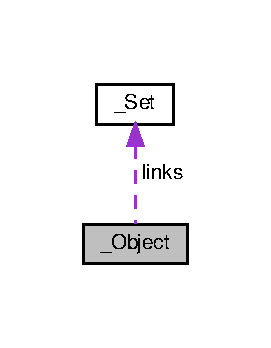
\includegraphics[width=130pt]{struct__Object__coll__graph}
\end{center}
\end{figure}
\subsection*{Data Fields}
\begin{DoxyCompactItemize}
\item 
\hyperlink{types_8h_a845e604fb28f7e3d97549da3448149d3}{Id} \hyperlink{struct__Object_a3cff7a0e8dc4e9d23895ed9af1b7653a}{id}
\item 
char $\ast$ \hyperlink{struct__Object_ab2d033c018fbe2639c88561e55306832}{ldescrp}
\item 
char \hyperlink{struct__Object_a59556463a256cec309077768589f10a8}{name} \mbox{[}\hyperlink{object_8h_a6a2f391825e94d06a3137b75abfa1bba}{M\+A\+X\+\_\+\+O\+B\+J\+\_\+\+N\+A\+ME}\mbox{]}
\item 
char \hyperlink{struct__Object_affa493ad8fdeafe924950f7388356a55}{descrp} \mbox{[}\hyperlink{object_8h_a9c396da2f3b9f0191120ff1666af6381}{M\+A\+X\+\_\+\+O\+B\+J\+\_\+\+D\+E\+S\+C\+RP}\mbox{]}
\item 
long \hyperlink{struct__Object_a9074217e572100d1259487a818bb0a0a}{attr} \mbox{[}\hyperlink{object_8h_a6b252b064231d7dc71c194dfea24b32b}{M\+A\+X\+\_\+\+O\+B\+J\+\_\+\+A\+T\+T\+RS}\mbox{]}
\item 
\hyperlink{set_8h_a6d3b7f7c92cbb4577ef3ef7ddbf93161}{Set} $\ast$ \hyperlink{struct__Object_afd29bc78dd0fc104db1aab87c6fc7d5c}{links}
\end{DoxyCompactItemize}


\subsection{Detailed Description}
Main object structure. 

This structure defines an object whose fields are an id and a name 

\subsection{Field Documentation}
\mbox{\Hypertarget{struct__Object_a3cff7a0e8dc4e9d23895ed9af1b7653a}\label{struct__Object_a3cff7a0e8dc4e9d23895ed9af1b7653a}} 
\index{\+\_\+\+Object@{\+\_\+\+Object}!id@{id}}
\index{id@{id}!\+\_\+\+Object@{\+\_\+\+Object}}
\subsubsection{\texorpdfstring{id}{id}}
{\footnotesize\ttfamily \hyperlink{types_8h_a845e604fb28f7e3d97549da3448149d3}{Id} \+\_\+\+Object\+::id}

Identifier \mbox{\Hypertarget{struct__Object_ab2d033c018fbe2639c88561e55306832}\label{struct__Object_ab2d033c018fbe2639c88561e55306832}} 
\index{\+\_\+\+Object@{\+\_\+\+Object}!ldescrp@{ldescrp}}
\index{ldescrp@{ldescrp}!\+\_\+\+Object@{\+\_\+\+Object}}
\subsubsection{\texorpdfstring{ldescrp}{ldescrp}}
{\footnotesize\ttfamily char$\ast$ \+\_\+\+Object\+::ldescrp}

Long description of the object \mbox{\Hypertarget{struct__Object_a59556463a256cec309077768589f10a8}\label{struct__Object_a59556463a256cec309077768589f10a8}} 
\index{\+\_\+\+Object@{\+\_\+\+Object}!name@{name}}
\index{name@{name}!\+\_\+\+Object@{\+\_\+\+Object}}
\subsubsection{\texorpdfstring{name}{name}}
{\footnotesize\ttfamily char \+\_\+\+Object\+::name\mbox{[}\hyperlink{object_8h_a6a2f391825e94d06a3137b75abfa1bba}{M\+A\+X\+\_\+\+O\+B\+J\+\_\+\+N\+A\+ME}\mbox{]}}

Object\textquotesingle{}s name \mbox{\Hypertarget{struct__Object_affa493ad8fdeafe924950f7388356a55}\label{struct__Object_affa493ad8fdeafe924950f7388356a55}} 
\index{\+\_\+\+Object@{\+\_\+\+Object}!descrp@{descrp}}
\index{descrp@{descrp}!\+\_\+\+Object@{\+\_\+\+Object}}
\subsubsection{\texorpdfstring{descrp}{descrp}}
{\footnotesize\ttfamily char \+\_\+\+Object\+::descrp\mbox{[}\hyperlink{object_8h_a9c396da2f3b9f0191120ff1666af6381}{M\+A\+X\+\_\+\+O\+B\+J\+\_\+\+D\+E\+S\+C\+RP}\mbox{]}}

Object\textquotesingle{}s description \mbox{\Hypertarget{struct__Object_a9074217e572100d1259487a818bb0a0a}\label{struct__Object_a9074217e572100d1259487a818bb0a0a}} 
\index{\+\_\+\+Object@{\+\_\+\+Object}!attr@{attr}}
\index{attr@{attr}!\+\_\+\+Object@{\+\_\+\+Object}}
\subsubsection{\texorpdfstring{attr}{attr}}
{\footnotesize\ttfamily long \+\_\+\+Object\+::attr\mbox{[}\hyperlink{object_8h_a6b252b064231d7dc71c194dfea24b32b}{M\+A\+X\+\_\+\+O\+B\+J\+\_\+\+A\+T\+T\+RS}\mbox{]}}

Object attributes \mbox{\Hypertarget{struct__Object_afd29bc78dd0fc104db1aab87c6fc7d5c}\label{struct__Object_afd29bc78dd0fc104db1aab87c6fc7d5c}} 
\index{\+\_\+\+Object@{\+\_\+\+Object}!links@{links}}
\index{links@{links}!\+\_\+\+Object@{\+\_\+\+Object}}
\subsubsection{\texorpdfstring{links}{links}}
{\footnotesize\ttfamily \hyperlink{set_8h_a6d3b7f7c92cbb4577ef3ef7ddbf93161}{Set}$\ast$ \+\_\+\+Object\+::links}

Links that the object can open 

The documentation for this struct was generated from the following file\+:\begin{DoxyCompactItemize}
\item 
src/\hyperlink{object_8c}{object.\+c}\end{DoxyCompactItemize}

\hypertarget{struct__Player}{}\section{\+\_\+\+Player Struct Reference}
\label{struct__Player}\index{\+\_\+\+Player@{\+\_\+\+Player}}


Player\textquotesingle{}s structure.  




Collaboration diagram for \+\_\+\+Player\+:\nopagebreak
\begin{figure}[H]
\begin{center}
\leavevmode
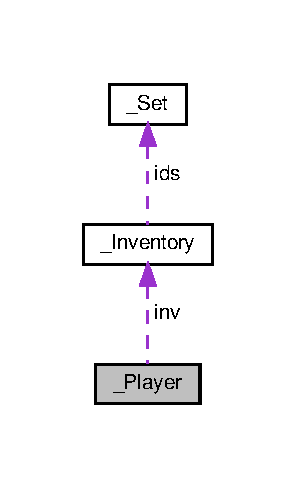
\includegraphics[width=142pt]{struct__Player__coll__graph}
\end{center}
\end{figure}
\subsection*{Data Fields}
\begin{DoxyCompactItemize}
\item 
\mbox{\Hypertarget{struct__Player_a60d635cd063816a9c1bd873f4868bb90}\label{struct__Player_a60d635cd063816a9c1bd873f4868bb90}} 
\hyperlink{types_8h_a845e604fb28f7e3d97549da3448149d3}{Id} \hyperlink{struct__Player_a60d635cd063816a9c1bd873f4868bb90}{id}
\begin{DoxyCompactList}\small\item\em P\+Layer\textquotesingle{}s Identifier. \end{DoxyCompactList}\item 
\mbox{\Hypertarget{struct__Player_a40f39335ccf0d2de882b7588f1917e58}\label{struct__Player_a40f39335ccf0d2de882b7588f1917e58}} 
\hyperlink{types_8h_a845e604fb28f7e3d97549da3448149d3}{Id} \hyperlink{struct__Player_a40f39335ccf0d2de882b7588f1917e58}{loc}
\begin{DoxyCompactList}\small\item\em Player\textquotesingle{}s location. \end{DoxyCompactList}\item 
\mbox{\Hypertarget{struct__Player_aaaeeb03326c37ce62c333c2b94fde23c}\label{struct__Player_aaaeeb03326c37ce62c333c2b94fde23c}} 
\hyperlink{inventory_8h_a2253bf64ac4ce6a9c1d6f39c0b0d32a3}{Inventory} $\ast$ \hyperlink{struct__Player_aaaeeb03326c37ce62c333c2b94fde23c}{inv}
\begin{DoxyCompactList}\small\item\em Player\textquotesingle{}s inventory. \end{DoxyCompactList}\item 
\mbox{\Hypertarget{struct__Player_ac89715f913cc607b75eb7236765c41f5}\label{struct__Player_ac89715f913cc607b75eb7236765c41f5}} 
char \hyperlink{struct__Player_ac89715f913cc607b75eb7236765c41f5}{name} \mbox{[}\hyperlink{types_8h_a92ed8507d1cd2331ad09275c5c4c1c89}{W\+O\+R\+D\+\_\+\+S\+I\+ZE}+1\mbox{]}
\begin{DoxyCompactList}\small\item\em Player\textquotesingle{}s name. \end{DoxyCompactList}\end{DoxyCompactItemize}


\subsection{Detailed Description}
Player\textquotesingle{}s structure. 

This structure defines an player whose fields are an id, a name, a location and an inventary of objects 

The documentation for this struct was generated from the following file\+:\begin{DoxyCompactItemize}
\item 
src/\hyperlink{player_8c}{player.\+c}\end{DoxyCompactItemize}

\hypertarget{struct__Set}{}\section{\+\_\+\+Set Struct Reference}
\label{struct__Set}\index{\+\_\+\+Set@{\+\_\+\+Set}}


Set structure.  


\subsection*{Data Fields}
\begin{DoxyCompactItemize}
\item 
\mbox{\Hypertarget{struct__Set_a3b2034bbfee5ca2b0dde5b6073c264cc}\label{struct__Set_a3b2034bbfee5ca2b0dde5b6073c264cc}} 
\hyperlink{types_8h_a845e604fb28f7e3d97549da3448149d3}{Id} \hyperlink{struct__Set_a3b2034bbfee5ca2b0dde5b6073c264cc}{ids} \mbox{[}\hyperlink{set_8h_abc21882f4958e6b56aaf2f3c18f80d43}{M\+A\+X\+\_\+\+S\+ET}\mbox{]}
\begin{DoxyCompactList}\small\item\em Array of id\textquotesingle{}s. \end{DoxyCompactList}\item 
\mbox{\Hypertarget{struct__Set_a9ae5f2cab9df62f0a98dd683be804878}\label{struct__Set_a9ae5f2cab9df62f0a98dd683be804878}} 
int \hyperlink{struct__Set_a9ae5f2cab9df62f0a98dd683be804878}{total}
\begin{DoxyCompactList}\small\item\em Total number of id\textquotesingle{}s. \end{DoxyCompactList}\end{DoxyCompactItemize}


\subsection{Detailed Description}
Set structure. 

The documentation for this struct was generated from the following file\+:\begin{DoxyCompactItemize}
\item 
src/set.\+c\end{DoxyCompactItemize}

\hypertarget{struct__Space}{}\section{\+\_\+\+Space Struct Reference}
\label{struct__Space}\index{\+\_\+\+Space@{\+\_\+\+Space}}


Space structure.  


\subsection*{Data Fields}
\begin{DoxyCompactItemize}
\item 
\mbox{\Hypertarget{struct__Space_a70cb461deb9ac073e401b607339b567f}\label{struct__Space_a70cb461deb9ac073e401b607339b567f}} 
Id \hyperlink{struct__Space_a70cb461deb9ac073e401b607339b567f}{id}
\begin{DoxyCompactList}\small\item\em Space id. \end{DoxyCompactList}\item 
\mbox{\Hypertarget{struct__Space_ae5ebe53ce79514d7d2d93911e0159252}\label{struct__Space_ae5ebe53ce79514d7d2d93911e0159252}} 
Id \hyperlink{struct__Space_ae5ebe53ce79514d7d2d93911e0159252}{north}
\begin{DoxyCompactList}\small\item\em Space north id. \end{DoxyCompactList}\item 
\mbox{\Hypertarget{struct__Space_a646b68c22a0bbf1685033c96109d31d1}\label{struct__Space_a646b68c22a0bbf1685033c96109d31d1}} 
Id \hyperlink{struct__Space_a646b68c22a0bbf1685033c96109d31d1}{south}
\begin{DoxyCompactList}\small\item\em Space south id. \end{DoxyCompactList}\item 
\mbox{\Hypertarget{struct__Space_a41ce2bf33cf0c157b358221f094ee05b}\label{struct__Space_a41ce2bf33cf0c157b358221f094ee05b}} 
Id \hyperlink{struct__Space_a41ce2bf33cf0c157b358221f094ee05b}{east}
\begin{DoxyCompactList}\small\item\em Space east id. \end{DoxyCompactList}\item 
\mbox{\Hypertarget{struct__Space_a20c1d259e93b44e24ba82982e142eb9b}\label{struct__Space_a20c1d259e93b44e24ba82982e142eb9b}} 
Id \hyperlink{struct__Space_a20c1d259e93b44e24ba82982e142eb9b}{west}
\begin{DoxyCompactList}\small\item\em Space west id. \end{DoxyCompactList}\item 
\mbox{\Hypertarget{struct__Space_ad69773f9a031624255530244436a211f}\label{struct__Space_ad69773f9a031624255530244436a211f}} 
char \hyperlink{struct__Space_ad69773f9a031624255530244436a211f}{name} \mbox{[}M\+A\+X\+\_\+\+S\+P\+A\+C\+E\+\_\+\+N\+A\+ME\mbox{]}
\begin{DoxyCompactList}\small\item\em Space name. \end{DoxyCompactList}\item 
\mbox{\Hypertarget{struct__Space_a661ed8b0fc8085b6db70188aa5085625}\label{struct__Space_a661ed8b0fc8085b6db70188aa5085625}} 
Set $\ast$ \hyperlink{struct__Space_a661ed8b0fc8085b6db70188aa5085625}{objects}
\begin{DoxyCompactList}\small\item\em Set of objects in the space. \end{DoxyCompactList}\item 
\mbox{\Hypertarget{struct__Space_ab4b3f4af835727b6afe807d2aded4ff2}\label{struct__Space_ab4b3f4af835727b6afe807d2aded4ff2}} 
char \hyperlink{struct__Space_ab4b3f4af835727b6afe807d2aded4ff2}{picture} \mbox{[}P\+I\+C\+T\+U\+R\+E\+\_\+\+L\+EN\mbox{]}
\begin{DoxyCompactList}\small\item\em Space structure. \end{DoxyCompactList}\end{DoxyCompactItemize}


\subsection{Detailed Description}
Space structure. 

$<$ 

The documentation for this struct was generated from the following file\+:\begin{DoxyCompactItemize}
\item 
src/\hyperlink{space_8c}{space.\+c}\end{DoxyCompactItemize}

\hypertarget{struct__Ui}{}\section{\+\_\+\+Ui Struct Reference}
\label{struct__Ui}\index{\+\_\+\+Ui@{\+\_\+\+Ui}}


Main UI structure.  




Collaboration diagram for \+\_\+\+Ui\+:\nopagebreak
\begin{figure}[H]
\begin{center}
\leavevmode
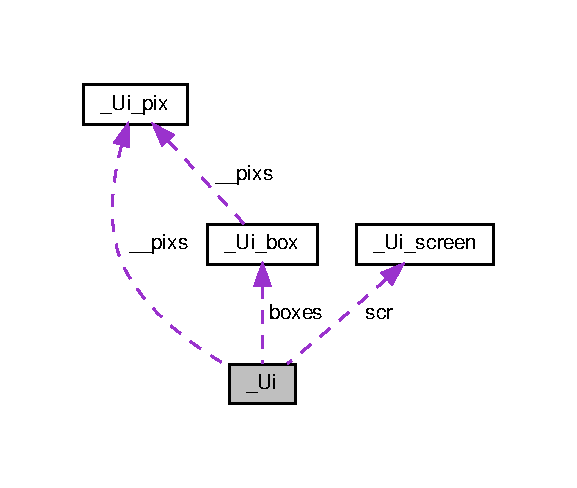
\includegraphics[width=277pt]{struct__Ui__coll__graph}
\end{center}
\end{figure}
\subsection*{Data Fields}
\begin{DoxyCompactItemize}
\item 
\mbox{\Hypertarget{struct__Ui_abd7c2a78bbdbe0e91a47a1461660b747}\label{struct__Ui_abd7c2a78bbdbe0e91a47a1461660b747}} 
\hyperlink{struct__Ui__screen}{Ui\+\_\+screen} \hyperlink{struct__Ui_abd7c2a78bbdbe0e91a47a1461660b747}{scr}
\begin{DoxyCompactList}\small\item\em Screen. \end{DoxyCompactList}\item 
\mbox{\Hypertarget{struct__Ui_ab4d33275d1afe8817a640653ab4b6848}\label{struct__Ui_ab4d33275d1afe8817a640653ab4b6848}} 
\hyperlink{struct__Ui__box}{Ui\+\_\+box} $\ast$ \hyperlink{struct__Ui_ab4d33275d1afe8817a640653ab4b6848}{boxes} \mbox{[}\hyperlink{ui_8c_a1be73fb0e5253951bdb7f2a4bd6a1524}{U\+I\+\_\+\+M\+A\+X\+\_\+\+B\+O\+X\+ES}\mbox{]}
\begin{DoxyCompactList}\small\item\em Boxes. \end{DoxyCompactList}\item 
\mbox{\Hypertarget{struct__Ui_a11af896bffe4bdbeca5ca871f7a9b7f0}\label{struct__Ui_a11af896bffe4bdbeca5ca871f7a9b7f0}} 
\hyperlink{struct__Ui__pix}{Ui\+\_\+pix} $\ast$$\ast$ \hyperlink{struct__Ui_a11af896bffe4bdbeca5ca871f7a9b7f0}{\+\_\+\+\_\+pixs}
\begin{DoxyCompactList}\small\item\em Pixels buffer. \end{DoxyCompactList}\item 
\mbox{\Hypertarget{struct__Ui_a368b423615ed2b6852c1ca99fd6351ce}\label{struct__Ui_a368b423615ed2b6852c1ca99fd6351ce}} 
int \hyperlink{struct__Ui_a368b423615ed2b6852c1ca99fd6351ce}{\+\_\+\+\_\+len}
\begin{DoxyCompactList}\small\item\em Number of pixels. \end{DoxyCompactList}\item 
\mbox{\Hypertarget{struct__Ui_a832844c64f4884883b541b3ce4f27106}\label{struct__Ui_a832844c64f4884883b541b3ce4f27106}} 
char \hyperlink{struct__Ui_a832844c64f4884883b541b3ce4f27106}{\+\_\+\+\_\+frm} \mbox{[}\hyperlink{ui_8c_aab208380ff579bef5fd8b91fa0c0215a}{U\+I\+\_\+\+M\+A\+X\+\_\+\+F\+R\+M\+\_\+\+L\+EN}\mbox{]}
\begin{DoxyCompactList}\small\item\em Temporary format. \end{DoxyCompactList}\end{DoxyCompactItemize}


\subsection{Detailed Description}
Main UI structure. 

The documentation for this struct was generated from the following file\+:\begin{DoxyCompactItemize}
\item 
src/\hyperlink{ui_8c}{ui.\+c}\end{DoxyCompactItemize}

\hypertarget{struct__Ui__box}{}\section{\+\_\+\+Ui\+\_\+box Struct Reference}
\label{struct__Ui__box}\index{\+\_\+\+Ui\+\_\+box@{\+\_\+\+Ui\+\_\+box}}


Main box structure.  




Collaboration diagram for \+\_\+\+Ui\+\_\+box\+:\nopagebreak
\begin{figure}[H]
\begin{center}
\leavevmode
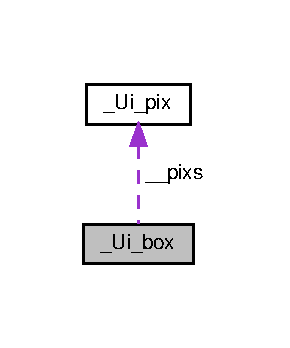
\includegraphics[width=139pt]{struct__Ui__box__coll__graph}
\end{center}
\end{figure}
\subsection*{Data Fields}
\begin{DoxyCompactItemize}
\item 
\mbox{\Hypertarget{struct__Ui__box_a03e07792d6c14766638d58e9e2edb844}\label{struct__Ui__box_a03e07792d6c14766638d58e9e2edb844}} 
\hyperlink{struct__Ui__pix}{Ui\+\_\+pix} $\ast$$\ast$ \hyperlink{struct__Ui__box_a03e07792d6c14766638d58e9e2edb844}{\+\_\+\+\_\+pixs}
\begin{DoxyCompactList}\small\item\em Pixels array. \end{DoxyCompactList}\item 
\mbox{\Hypertarget{struct__Ui__box_a4aa502d3b25a87a1465283d9ccc9fa77}\label{struct__Ui__box_a4aa502d3b25a87a1465283d9ccc9fa77}} 
int \hyperlink{struct__Ui__box_a4aa502d3b25a87a1465283d9ccc9fa77}{id}
\begin{DoxyCompactList}\small\item\em Box identification. \end{DoxyCompactList}\item 
\mbox{\Hypertarget{struct__Ui__box_a6e8c0df6554097fd1d0d0aa84d40ac29}\label{struct__Ui__box_a6e8c0df6554097fd1d0d0aa84d40ac29}} 
int \hyperlink{struct__Ui__box_a6e8c0df6554097fd1d0d0aa84d40ac29}{x}
\begin{DoxyCompactList}\small\item\em Coordenate x. \end{DoxyCompactList}\item 
\mbox{\Hypertarget{struct__Ui__box_a7bacb19580dcf6ece3ca60b64f62e459}\label{struct__Ui__box_a7bacb19580dcf6ece3ca60b64f62e459}} 
int \hyperlink{struct__Ui__box_a7bacb19580dcf6ece3ca60b64f62e459}{y}
\begin{DoxyCompactList}\small\item\em Coordenate y. \end{DoxyCompactList}\item 
\mbox{\Hypertarget{struct__Ui__box_a90f1e8d481ccbf0cc06e3bbb1c12b386}\label{struct__Ui__box_a90f1e8d481ccbf0cc06e3bbb1c12b386}} 
int \hyperlink{struct__Ui__box_a90f1e8d481ccbf0cc06e3bbb1c12b386}{w}
\begin{DoxyCompactList}\small\item\em Width. \end{DoxyCompactList}\item 
\mbox{\Hypertarget{struct__Ui__box_ab81930762400818df39bd6acc348d26f}\label{struct__Ui__box_ab81930762400818df39bd6acc348d26f}} 
int \hyperlink{struct__Ui__box_ab81930762400818df39bd6acc348d26f}{h}
\begin{DoxyCompactList}\small\item\em Height. \end{DoxyCompactList}\item 
\mbox{\Hypertarget{struct__Ui__box_aa44d253872cfb9297e3fa71b93d9fc88}\label{struct__Ui__box_aa44d253872cfb9297e3fa71b93d9fc88}} 
int \hyperlink{struct__Ui__box_aa44d253872cfb9297e3fa71b93d9fc88}{cx}
\begin{DoxyCompactList}\small\item\em Position of the x cursor. \end{DoxyCompactList}\item 
\mbox{\Hypertarget{struct__Ui__box_a993ecc3e3509632642cb403b731d9a6d}\label{struct__Ui__box_a993ecc3e3509632642cb403b731d9a6d}} 
int \hyperlink{struct__Ui__box_a993ecc3e3509632642cb403b731d9a6d}{cy}
\begin{DoxyCompactList}\small\item\em Position of the y cursor. \end{DoxyCompactList}\item 
\mbox{\Hypertarget{struct__Ui__box_ade30a16b2e23d494a77767ce516f00d9}\label{struct__Ui__box_ade30a16b2e23d494a77767ce516f00d9}} 
int \hyperlink{struct__Ui__box_ade30a16b2e23d494a77767ce516f00d9}{\+\_\+\+\_\+len}
\begin{DoxyCompactList}\small\item\em Length of the pixels array. \end{DoxyCompactList}\item 
\mbox{\Hypertarget{struct__Ui__box_a4030a2fd2487e5a4cde2b4fccc999166}\label{struct__Ui__box_a4030a2fd2487e5a4cde2b4fccc999166}} 
int \hyperlink{struct__Ui__box_a4030a2fd2487e5a4cde2b4fccc999166}{pad} \mbox{[}4\mbox{]}
\begin{DoxyCompactList}\small\item\em Box padding. \end{DoxyCompactList}\item 
\mbox{\Hypertarget{struct__Ui__box_a2562527c18b6318ba537faae8dd2d06c}\label{struct__Ui__box_a2562527c18b6318ba537faae8dd2d06c}} 
\hyperlink{ui_8h_ab87bacfdad76e61b9412d7124be44c1c}{Color} \hyperlink{struct__Ui__box_a2562527c18b6318ba537faae8dd2d06c}{bg}
\begin{DoxyCompactList}\small\item\em Background color. \end{DoxyCompactList}\end{DoxyCompactItemize}


\subsection{Detailed Description}
Main box structure. 

The documentation for this struct was generated from the following file\+:\begin{DoxyCompactItemize}
\item 
src/ui.\+c\end{DoxyCompactItemize}

\hypertarget{struct__Ui__pix}{}\section{\+\_\+\+Ui\+\_\+pix Struct Reference}
\label{struct__Ui__pix}\index{\+\_\+\+Ui\+\_\+pix@{\+\_\+\+Ui\+\_\+pix}}


Basic pixel structure.  


\subsection*{Data Fields}
\begin{DoxyCompactItemize}
\item 
\mbox{\Hypertarget{struct__Ui__pix_aa12b962b28524e2f295d0fd90b9595a8}\label{struct__Ui__pix_aa12b962b28524e2f295d0fd90b9595a8}} 
char \hyperlink{struct__Ui__pix_aa12b962b28524e2f295d0fd90b9595a8}{c}
\begin{DoxyCompactList}\small\item\em Pixel char. \end{DoxyCompactList}\item 
\mbox{\Hypertarget{struct__Ui__pix_a139bbde94a87ff7907f964e27db4620a}\label{struct__Ui__pix_a139bbde94a87ff7907f964e27db4620a}} 
int {\bfseries frm} \mbox{[}U\+I\+\_\+\+M\+A\+X\+\_\+\+F\+RM\mbox{]}
\end{DoxyCompactItemize}


\subsection{Detailed Description}
Basic pixel structure. 

The documentation for this struct was generated from the following file\+:\begin{DoxyCompactItemize}
\item 
src/\hyperlink{ui_8c}{ui.\+c}\end{DoxyCompactItemize}

\hypertarget{struct__Ui__screen}{}\section{\+\_\+\+Ui\+\_\+screen Struct Reference}
\label{struct__Ui__screen}\index{\+\_\+\+Ui\+\_\+screen@{\+\_\+\+Ui\+\_\+screen}}


Main UI screen structure.  


\subsection*{Data Fields}
\begin{DoxyCompactItemize}
\item 
\mbox{\Hypertarget{struct__Ui__screen_a0d1d60ef32f78df18ce4f7ac8b97e5ea}\label{struct__Ui__screen_a0d1d60ef32f78df18ce4f7ac8b97e5ea}} 
int \hyperlink{struct__Ui__screen_a0d1d60ef32f78df18ce4f7ac8b97e5ea}{w}
\begin{DoxyCompactList}\small\item\em Width. \end{DoxyCompactList}\item 
\mbox{\Hypertarget{struct__Ui__screen_ad16a11cf58cfd3423e7b5e9b2fa184e3}\label{struct__Ui__screen_ad16a11cf58cfd3423e7b5e9b2fa184e3}} 
int \hyperlink{struct__Ui__screen_ad16a11cf58cfd3423e7b5e9b2fa184e3}{h}
\begin{DoxyCompactList}\small\item\em Height. \end{DoxyCompactList}\end{DoxyCompactItemize}


\subsection{Detailed Description}
Main UI screen structure. 

The documentation for this struct was generated from the following file\+:\begin{DoxyCompactItemize}
\item 
src/\hyperlink{ui_8c}{ui.\+c}\end{DoxyCompactItemize}

\chapter{File Documentation}
\hypertarget{cmd_8h}{}\section{src/cmd.h File Reference}
\label{cmd_8h}\index{src/cmd.\+h@{src/cmd.\+h}}


Command interpreter.  


{\ttfamily \#include \char`\"{}types.\+h\char`\"{}}\newline
Include dependency graph for cmd.\+h\+:\nopagebreak
\begin{figure}[H]
\begin{center}
\leavevmode
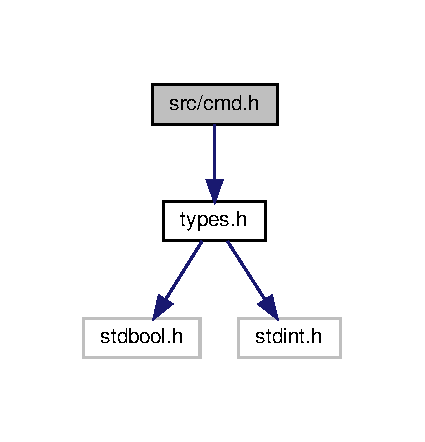
\includegraphics[width=204pt]{cmd_8h__incl}
\end{center}
\end{figure}
This graph shows which files directly or indirectly include this file\+:\nopagebreak
\begin{figure}[H]
\begin{center}
\leavevmode
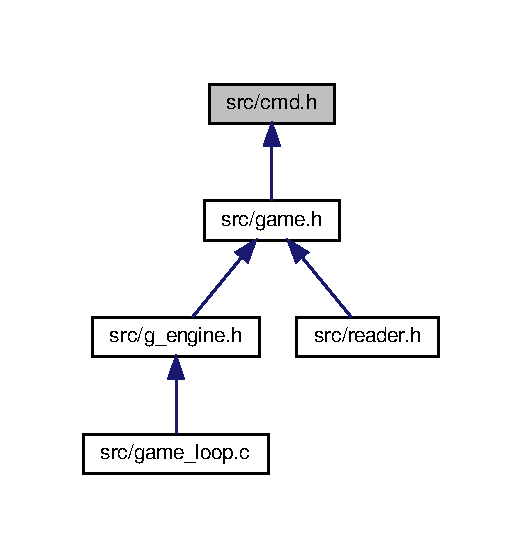
\includegraphics[width=251pt]{cmd_8h__dep__incl}
\end{center}
\end{figure}
\subsection*{Macros}
\begin{DoxyCompactItemize}
\item 
\mbox{\Hypertarget{cmd_8h_a1eb73c104b484cf18752169509cebfe2}\label{cmd_8h_a1eb73c104b484cf18752169509cebfe2}} 
\#define \hyperlink{cmd_8h_a1eb73c104b484cf18752169509cebfe2}{M\+A\+X\+\_\+\+C\+M\+D\+\_\+\+L\+EN}~50
\begin{DoxyCompactList}\small\item\em Maximum command length. \end{DoxyCompactList}\item 
\mbox{\Hypertarget{cmd_8h_ad14effda14501a769b3d46984d43aa00}\label{cmd_8h_ad14effda14501a769b3d46984d43aa00}} 
\#define \hyperlink{cmd_8h_ad14effda14501a769b3d46984d43aa00}{M\+A\+X\+\_\+\+C\+M\+DS}~15
\begin{DoxyCompactList}\small\item\em Maximum quantity of commands. \end{DoxyCompactList}\item 
\mbox{\Hypertarget{cmd_8h_a64bf1979142baf43271722ff7b14c17d}\label{cmd_8h_a64bf1979142baf43271722ff7b14c17d}} 
\#define \hyperlink{cmd_8h_a64bf1979142baf43271722ff7b14c17d}{M\+A\+X\+\_\+\+C\+M\+D\+\_\+\+A\+R\+GC}~5
\begin{DoxyCompactList}\small\item\em Maximum command arguments. \end{DoxyCompactList}\item 
\mbox{\Hypertarget{cmd_8h_ab972c58772002197942552cc47b6b5cd}\label{cmd_8h_ab972c58772002197942552cc47b6b5cd}} 
\#define \hyperlink{cmd_8h_ab972c58772002197942552cc47b6b5cd}{M\+A\+X\+\_\+\+C\+M\+D\+\_\+\+A\+NS}~200
\begin{DoxyCompactList}\small\item\em Maximum command answer length. \end{DoxyCompactList}\item 
\mbox{\Hypertarget{cmd_8h_a536329c6bdf286710c20c6dd9a0750cc}\label{cmd_8h_a536329c6bdf286710c20c6dd9a0750cc}} 
\#define \hyperlink{cmd_8h_a536329c6bdf286710c20c6dd9a0750cc}{M\+A\+X\+\_\+\+C\+M\+D\+\_\+\+IN}~100
\begin{DoxyCompactList}\small\item\em Maximum command input length. \end{DoxyCompactList}\end{DoxyCompactItemize}
\subsection*{Typedefs}
\begin{DoxyCompactItemize}
\item 
\mbox{\Hypertarget{cmd_8h_a2933336e1f8003400f3b050402f0f5f3}\label{cmd_8h_a2933336e1f8003400f3b050402f0f5f3}} 
typedef enum \hyperlink{cmd_8h_a00a332e55439547f3ed90d0839bd1995}{enum\+\_\+\+Cid} \hyperlink{cmd_8h_a2933336e1f8003400f3b050402f0f5f3}{Cid}
\begin{DoxyCompactList}\small\item\em Command identification. \end{DoxyCompactList}\item 
\mbox{\Hypertarget{cmd_8h_a78d7a8bd781b5514e6dd7e1253bb1907}\label{cmd_8h_a78d7a8bd781b5514e6dd7e1253bb1907}} 
typedef void($\ast$ \hyperlink{cmd_8h_a78d7a8bd781b5514e6dd7e1253bb1907}{cmd\+\_\+fn}) (void $\ast$)
\begin{DoxyCompactList}\small\item\em Command callback. \end{DoxyCompactList}\item 
\mbox{\Hypertarget{cmd_8h_ab2b68b94b84c77ba11a699a76b8cf9cc}\label{cmd_8h_ab2b68b94b84c77ba11a699a76b8cf9cc}} 
typedef struct \hyperlink{struct__Cmd}{\+\_\+\+Cmd} {\bfseries Cmd}
\end{DoxyCompactItemize}
\subsection*{Enumerations}
\begin{DoxyCompactItemize}
\item 
enum \hyperlink{cmd_8h_a00a332e55439547f3ed90d0839bd1995}{enum\+\_\+\+Cid} \{ \newline
\hyperlink{cmd_8h_a00a332e55439547f3ed90d0839bd1995a6ce26a62afab55d7606ad4e92428b30c}{U\+N\+K\+N\+O\+WN}, 
\hyperlink{cmd_8h_a00a332e55439547f3ed90d0839bd1995a7a10b5d68d31711288e1fe0fa17dbf4f}{E\+X\+IT}, 
\hyperlink{cmd_8h_a00a332e55439547f3ed90d0839bd1995ab13b96bf99a409e019f70dc1602532fd}{N\+E\+XT}, 
\hyperlink{cmd_8h_a00a332e55439547f3ed90d0839bd1995ac921ff2cfc571c1d19b0485d7f6926ee}{B\+A\+CK}, 
\newline
\hyperlink{cmd_8h_a00a332e55439547f3ed90d0839bd1995a7405647410e343caba1bf383e83d4f5f}{T\+A\+KE}, 
\hyperlink{cmd_8h_a00a332e55439547f3ed90d0839bd1995a8b0b0025af76a3d8f0b7b1d4758e51a6}{D\+R\+OP}, 
\hyperlink{cmd_8h_a00a332e55439547f3ed90d0839bd1995a2eeb9fef8a6a516fa6437a44a6efbd52}{R\+O\+LL}, 
\hyperlink{cmd_8h_a00a332e55439547f3ed90d0839bd1995adb45120aafd37a973140edee24708065}{L\+E\+FT}, 
\newline
\hyperlink{cmd_8h_a00a332e55439547f3ed90d0839bd1995aec8379af7490bb9eaaf579cf17876f38}{R\+I\+G\+HT}
 \}\begin{DoxyCompactList}\small\item\em Command identification. \end{DoxyCompactList}
\end{DoxyCompactItemize}
\subsection*{Functions}
\begin{DoxyCompactItemize}
\item 
void \hyperlink{cmd_8h_ab2829bf716f494548177511118bf6c5b}{cmd\+\_\+set} (\hyperlink{cmd_8h_a2933336e1f8003400f3b050402f0f5f3}{Cid} id, const char $\ast$b\+\_\+name, const char $\ast$s\+\_\+name, \hyperlink{cmd_8h_a78d7a8bd781b5514e6dd7e1253bb1907}{cmd\+\_\+fn} fn)
\begin{DoxyCompactList}\small\item\em Sets up a new command and stores it inside a private array. \end{DoxyCompactList}\item 
\hyperlink{struct__Cmd}{Cmd} $\ast$ \hyperlink{cmd_8h_a511ba687ae937a7eb95ea06b79b2b8ec}{cmd\+\_\+get} (\hyperlink{cmd_8h_a2933336e1f8003400f3b050402f0f5f3}{Cid} id)
\begin{DoxyCompactList}\small\item\em Sets a command by its id. \end{DoxyCompactList}\item 
\mbox{\Hypertarget{cmd_8h_a3078f0effe67b212b1b913e3ff0c08dc}\label{cmd_8h_a3078f0effe67b212b1b913e3ff0c08dc}} 
void \hyperlink{cmd_8h_a3078f0effe67b212b1b913e3ff0c08dc}{cmd\+\_\+free} ()
\begin{DoxyCompactList}\small\item\em Destroy all the setted commands. \end{DoxyCompactList}\item 
\hyperlink{struct__Cmd}{Cmd} $\ast$ \hyperlink{cmd_8h_abb04779da8a594a45843a10b91e9e3a3}{cmd\+\_\+req} ()
\begin{DoxyCompactList}\small\item\em Requests a new command from stdin. \end{DoxyCompactList}\item 
void \hyperlink{cmd_8h_a5090e929f5e97aa5492b47dfd7a6ec91}{cmd\+\_\+cb} (\hyperlink{struct__Cmd}{Cmd} $\ast$cmd, void $\ast$vp)
\begin{DoxyCompactList}\small\item\em Calls to the callback function stored in the given command. \end{DoxyCompactList}\item 
void \hyperlink{cmd_8h_aefbbd086c6cc093159c8dcc077363a31}{cmd\+\_\+set\+\_\+ans} (\hyperlink{struct__Cmd}{Cmd} $\ast$cmd, int errc, const char $\ast$str,...)
\begin{DoxyCompactList}\small\item\em Sets an answer to the given command. \end{DoxyCompactList}\item 
const char $\ast$ \hyperlink{cmd_8h_a9fc56f507a2e6dabe93d8e8e03a81164}{cmd\+\_\+get\+\_\+ans} (\hyperlink{struct__Cmd}{Cmd} $\ast$cmd)
\begin{DoxyCompactList}\small\item\em Gets a previus answer of the given command. \end{DoxyCompactList}\item 
const char $\ast$ \hyperlink{cmd_8h_aa1e02137469ddc06fa9bcb3dac2c3a56}{cmd\+\_\+get\+\_\+argv} (\hyperlink{struct__Cmd}{Cmd} $\ast$cmd, int idx)
\begin{DoxyCompactList}\small\item\em Gets the desired indexed argument. \end{DoxyCompactList}\item 
const int \hyperlink{cmd_8h_a45b6622fba552dd2b1c620afb4af451c}{cmd\+\_\+get\+\_\+argc} (\hyperlink{struct__Cmd}{Cmd} $\ast$cmd)
\begin{DoxyCompactList}\small\item\em Gets the number of arguemnts of a given command. \end{DoxyCompactList}\item 
const int \hyperlink{cmd_8h_a57baf1963c86de1643043f9c4cee9567}{cmd\+\_\+get\+\_\+errc} (\hyperlink{struct__Cmd}{Cmd} $\ast$cmd)
\begin{DoxyCompactList}\small\item\em Gets the error code of a given command. \end{DoxyCompactList}\item 
const \hyperlink{cmd_8h_a2933336e1f8003400f3b050402f0f5f3}{Cid} \hyperlink{cmd_8h_a399883b5394d12f2c19816e72a756245}{cmd\+\_\+get\+\_\+cid} (\hyperlink{struct__Cmd}{Cmd} $\ast$cmd)
\begin{DoxyCompactList}\small\item\em Gets the command id. \end{DoxyCompactList}\item 
const char $\ast$ \hyperlink{cmd_8h_afc6f99e63609bd15653ea164fbe59ede}{cmd\+\_\+get\+\_\+bname} (\hyperlink{struct__Cmd}{Cmd} $\ast$cmd)
\begin{DoxyCompactList}\small\item\em Gets the base name of a given command. \end{DoxyCompactList}\item 
const char $\ast$ \hyperlink{cmd_8h_aa3bd4090b15be64bd3d4839233f85ee9}{cmd\+\_\+get\+\_\+sname} (\hyperlink{struct__Cmd}{Cmd} $\ast$cmd)
\begin{DoxyCompactList}\small\item\em Gets the short name of a given command. \end{DoxyCompactList}\end{DoxyCompactItemize}


\subsection{Detailed Description}
Command interpreter. 

\begin{DoxyAuthor}{Author}
Javier Romera 
\end{DoxyAuthor}
\begin{DoxyVersion}{Version}
0.\+8.\+3 
\end{DoxyVersion}
\begin{DoxyDate}{Date}
14/03/2019 
\end{DoxyDate}
\begin{DoxyCopyright}{Copyright}
G\+NU Public License 
\end{DoxyCopyright}


\subsection{Enumeration Type Documentation}
\mbox{\Hypertarget{cmd_8h_a00a332e55439547f3ed90d0839bd1995}\label{cmd_8h_a00a332e55439547f3ed90d0839bd1995}} 
\index{cmd.\+h@{cmd.\+h}!enum\+\_\+\+Cid@{enum\+\_\+\+Cid}}
\index{enum\+\_\+\+Cid@{enum\+\_\+\+Cid}!cmd.\+h@{cmd.\+h}}
\subsubsection{\texorpdfstring{enum\+\_\+\+Cid}{enum\_Cid}}
{\footnotesize\ttfamily enum \hyperlink{cmd_8h_a00a332e55439547f3ed90d0839bd1995}{enum\+\_\+\+Cid}}



Command identification. 

\begin{DoxyEnumFields}{Enumerator}
\raisebox{\heightof{T}}[0pt][0pt]{\index{U\+N\+K\+N\+O\+WN@{U\+N\+K\+N\+O\+WN}!cmd.\+h@{cmd.\+h}}\index{cmd.\+h@{cmd.\+h}!U\+N\+K\+N\+O\+WN@{U\+N\+K\+N\+O\+WN}}}\mbox{\Hypertarget{cmd_8h_a00a332e55439547f3ed90d0839bd1995a6ce26a62afab55d7606ad4e92428b30c}\label{cmd_8h_a00a332e55439547f3ed90d0839bd1995a6ce26a62afab55d7606ad4e92428b30c}} 
U\+N\+K\+N\+O\+WN&Unknown command \\
\hline

\raisebox{\heightof{T}}[0pt][0pt]{\index{E\+X\+IT@{E\+X\+IT}!cmd.\+h@{cmd.\+h}}\index{cmd.\+h@{cmd.\+h}!E\+X\+IT@{E\+X\+IT}}}\mbox{\Hypertarget{cmd_8h_a00a332e55439547f3ed90d0839bd1995a7a10b5d68d31711288e1fe0fa17dbf4f}\label{cmd_8h_a00a332e55439547f3ed90d0839bd1995a7a10b5d68d31711288e1fe0fa17dbf4f}} 
E\+X\+IT&xit command \\
\hline

\raisebox{\heightof{T}}[0pt][0pt]{\index{N\+E\+XT@{N\+E\+XT}!cmd.\+h@{cmd.\+h}}\index{cmd.\+h@{cmd.\+h}!N\+E\+XT@{N\+E\+XT}}}\mbox{\Hypertarget{cmd_8h_a00a332e55439547f3ed90d0839bd1995ab13b96bf99a409e019f70dc1602532fd}\label{cmd_8h_a00a332e55439547f3ed90d0839bd1995ab13b96bf99a409e019f70dc1602532fd}} 
N\+E\+XT&Next command \\
\hline

\raisebox{\heightof{T}}[0pt][0pt]{\index{B\+A\+CK@{B\+A\+CK}!cmd.\+h@{cmd.\+h}}\index{cmd.\+h@{cmd.\+h}!B\+A\+CK@{B\+A\+CK}}}\mbox{\Hypertarget{cmd_8h_a00a332e55439547f3ed90d0839bd1995ac921ff2cfc571c1d19b0485d7f6926ee}\label{cmd_8h_a00a332e55439547f3ed90d0839bd1995ac921ff2cfc571c1d19b0485d7f6926ee}} 
B\+A\+CK&Back command \\
\hline

\raisebox{\heightof{T}}[0pt][0pt]{\index{T\+A\+KE@{T\+A\+KE}!cmd.\+h@{cmd.\+h}}\index{cmd.\+h@{cmd.\+h}!T\+A\+KE@{T\+A\+KE}}}\mbox{\Hypertarget{cmd_8h_a00a332e55439547f3ed90d0839bd1995a7405647410e343caba1bf383e83d4f5f}\label{cmd_8h_a00a332e55439547f3ed90d0839bd1995a7405647410e343caba1bf383e83d4f5f}} 
T\+A\+KE&Take command \\
\hline

\raisebox{\heightof{T}}[0pt][0pt]{\index{D\+R\+OP@{D\+R\+OP}!cmd.\+h@{cmd.\+h}}\index{cmd.\+h@{cmd.\+h}!D\+R\+OP@{D\+R\+OP}}}\mbox{\Hypertarget{cmd_8h_a00a332e55439547f3ed90d0839bd1995a8b0b0025af76a3d8f0b7b1d4758e51a6}\label{cmd_8h_a00a332e55439547f3ed90d0839bd1995a8b0b0025af76a3d8f0b7b1d4758e51a6}} 
D\+R\+OP&Drop command \\
\hline

\raisebox{\heightof{T}}[0pt][0pt]{\index{R\+O\+LL@{R\+O\+LL}!cmd.\+h@{cmd.\+h}}\index{cmd.\+h@{cmd.\+h}!R\+O\+LL@{R\+O\+LL}}}\mbox{\Hypertarget{cmd_8h_a00a332e55439547f3ed90d0839bd1995a2eeb9fef8a6a516fa6437a44a6efbd52}\label{cmd_8h_a00a332e55439547f3ed90d0839bd1995a2eeb9fef8a6a516fa6437a44a6efbd52}} 
R\+O\+LL&Roll command \\
\hline

\raisebox{\heightof{T}}[0pt][0pt]{\index{L\+E\+FT@{L\+E\+FT}!cmd.\+h@{cmd.\+h}}\index{cmd.\+h@{cmd.\+h}!L\+E\+FT@{L\+E\+FT}}}\mbox{\Hypertarget{cmd_8h_a00a332e55439547f3ed90d0839bd1995adb45120aafd37a973140edee24708065}\label{cmd_8h_a00a332e55439547f3ed90d0839bd1995adb45120aafd37a973140edee24708065}} 
L\+E\+FT&Left command \\
\hline

\raisebox{\heightof{T}}[0pt][0pt]{\index{R\+I\+G\+HT@{R\+I\+G\+HT}!cmd.\+h@{cmd.\+h}}\index{cmd.\+h@{cmd.\+h}!R\+I\+G\+HT@{R\+I\+G\+HT}}}\mbox{\Hypertarget{cmd_8h_a00a332e55439547f3ed90d0839bd1995aec8379af7490bb9eaaf579cf17876f38}\label{cmd_8h_a00a332e55439547f3ed90d0839bd1995aec8379af7490bb9eaaf579cf17876f38}} 
R\+I\+G\+HT&Right command \\
\hline

\end{DoxyEnumFields}


\subsection{Function Documentation}
\mbox{\Hypertarget{cmd_8h_ab2829bf716f494548177511118bf6c5b}\label{cmd_8h_ab2829bf716f494548177511118bf6c5b}} 
\index{cmd.\+h@{cmd.\+h}!cmd\+\_\+set@{cmd\+\_\+set}}
\index{cmd\+\_\+set@{cmd\+\_\+set}!cmd.\+h@{cmd.\+h}}
\subsubsection{\texorpdfstring{cmd\+\_\+set()}{cmd\_set()}}
{\footnotesize\ttfamily void cmd\+\_\+set (\begin{DoxyParamCaption}\item[{\hyperlink{cmd_8h_a2933336e1f8003400f3b050402f0f5f3}{Cid}}]{id,  }\item[{const char $\ast$}]{b\+\_\+name,  }\item[{const char $\ast$}]{s\+\_\+name,  }\item[{\hyperlink{cmd_8h_a78d7a8bd781b5514e6dd7e1253bb1907}{cmd\+\_\+fn}}]{fn }\end{DoxyParamCaption})}



Sets up a new command and stores it inside a private array. 


\begin{DoxyParams}{Parameters}
{\em \{\+Cid\}} & id -\/ Command identification \\
\hline
{\em \{char$\ast$\}} & b\+\_\+name -\/ The base name of the command \\
\hline
{\em \{char$\ast$\}} & s\+\_\+name -\/ The short name of the command \\
\hline
{\em \{cmd\+\_\+fn\}} & fn -\/ Command callback function \\
\hline
\end{DoxyParams}
\mbox{\Hypertarget{cmd_8h_a511ba687ae937a7eb95ea06b79b2b8ec}\label{cmd_8h_a511ba687ae937a7eb95ea06b79b2b8ec}} 
\index{cmd.\+h@{cmd.\+h}!cmd\+\_\+get@{cmd\+\_\+get}}
\index{cmd\+\_\+get@{cmd\+\_\+get}!cmd.\+h@{cmd.\+h}}
\subsubsection{\texorpdfstring{cmd\+\_\+get()}{cmd\_get()}}
{\footnotesize\ttfamily \hyperlink{struct__Cmd}{Cmd}$\ast$ cmd\+\_\+get (\begin{DoxyParamCaption}\item[{\hyperlink{cmd_8h_a2933336e1f8003400f3b050402f0f5f3}{Cid}}]{id }\end{DoxyParamCaption})}



Sets a command by its id. 


\begin{DoxyParams}{Parameters}
{\em \{\+Cid\}} & id -\/ Command identification \\
\hline
\end{DoxyParams}

\begin{DoxyRetVals}{Return values}
{\em -\/} & Command pointer \\
\hline
\end{DoxyRetVals}
\mbox{\Hypertarget{cmd_8h_abb04779da8a594a45843a10b91e9e3a3}\label{cmd_8h_abb04779da8a594a45843a10b91e9e3a3}} 
\index{cmd.\+h@{cmd.\+h}!cmd\+\_\+req@{cmd\+\_\+req}}
\index{cmd\+\_\+req@{cmd\+\_\+req}!cmd.\+h@{cmd.\+h}}
\subsubsection{\texorpdfstring{cmd\+\_\+req()}{cmd\_req()}}
{\footnotesize\ttfamily \hyperlink{struct__Cmd}{Cmd}$\ast$ cmd\+\_\+req (\begin{DoxyParamCaption}{ }\end{DoxyParamCaption})}



Requests a new command from stdin. 


\begin{DoxyRetVals}{Return values}
{\em -\/} & Returns a pointer of the parsed command \\
\hline
\end{DoxyRetVals}
\mbox{\Hypertarget{cmd_8h_a5090e929f5e97aa5492b47dfd7a6ec91}\label{cmd_8h_a5090e929f5e97aa5492b47dfd7a6ec91}} 
\index{cmd.\+h@{cmd.\+h}!cmd\+\_\+cb@{cmd\+\_\+cb}}
\index{cmd\+\_\+cb@{cmd\+\_\+cb}!cmd.\+h@{cmd.\+h}}
\subsubsection{\texorpdfstring{cmd\+\_\+cb()}{cmd\_cb()}}
{\footnotesize\ttfamily void cmd\+\_\+cb (\begin{DoxyParamCaption}\item[{\hyperlink{struct__Cmd}{Cmd} $\ast$}]{cmd,  }\item[{void $\ast$}]{vp }\end{DoxyParamCaption})}



Calls to the callback function stored in the given command. 


\begin{DoxyParams}{Parameters}
{\em \{\+Cmd$\ast$\}} & cmd -\/ Command pointer \\
\hline
\end{DoxyParams}
\mbox{\Hypertarget{cmd_8h_aefbbd086c6cc093159c8dcc077363a31}\label{cmd_8h_aefbbd086c6cc093159c8dcc077363a31}} 
\index{cmd.\+h@{cmd.\+h}!cmd\+\_\+set\+\_\+ans@{cmd\+\_\+set\+\_\+ans}}
\index{cmd\+\_\+set\+\_\+ans@{cmd\+\_\+set\+\_\+ans}!cmd.\+h@{cmd.\+h}}
\subsubsection{\texorpdfstring{cmd\+\_\+set\+\_\+ans()}{cmd\_set\_ans()}}
{\footnotesize\ttfamily void cmd\+\_\+set\+\_\+ans (\begin{DoxyParamCaption}\item[{\hyperlink{struct__Cmd}{Cmd} $\ast$}]{cmd,  }\item[{int}]{errc,  }\item[{const char $\ast$}]{str,  }\item[{}]{... }\end{DoxyParamCaption})}



Sets an answer to the given command. 


\begin{DoxyParams}{Parameters}
{\em \{\+Cmd$\ast$\}} & cmd -\/ Command pointer \\
\hline
{\em \{int\}} & errc -\/ Error code \\
\hline
{\em \{char$\ast$\}} & str -\/ String format \\
\hline
{\em \{...\}} & -\/ String format arguments \\
\hline
\end{DoxyParams}
\mbox{\Hypertarget{cmd_8h_a9fc56f507a2e6dabe93d8e8e03a81164}\label{cmd_8h_a9fc56f507a2e6dabe93d8e8e03a81164}} 
\index{cmd.\+h@{cmd.\+h}!cmd\+\_\+get\+\_\+ans@{cmd\+\_\+get\+\_\+ans}}
\index{cmd\+\_\+get\+\_\+ans@{cmd\+\_\+get\+\_\+ans}!cmd.\+h@{cmd.\+h}}
\subsubsection{\texorpdfstring{cmd\+\_\+get\+\_\+ans()}{cmd\_get\_ans()}}
{\footnotesize\ttfamily const char$\ast$ cmd\+\_\+get\+\_\+ans (\begin{DoxyParamCaption}\item[{\hyperlink{struct__Cmd}{Cmd} $\ast$}]{cmd }\end{DoxyParamCaption})}



Gets a previus answer of the given command. 


\begin{DoxyParams}{Parameters}
{\em \{\+Cmd$\ast$\}} & cmd -\/ Command pointer \\
\hline
\end{DoxyParams}

\begin{DoxyRetVals}{Return values}
{\em \{char$\ast$\}} & -\/ Command answer \\
\hline
\end{DoxyRetVals}
\mbox{\Hypertarget{cmd_8h_aa1e02137469ddc06fa9bcb3dac2c3a56}\label{cmd_8h_aa1e02137469ddc06fa9bcb3dac2c3a56}} 
\index{cmd.\+h@{cmd.\+h}!cmd\+\_\+get\+\_\+argv@{cmd\+\_\+get\+\_\+argv}}
\index{cmd\+\_\+get\+\_\+argv@{cmd\+\_\+get\+\_\+argv}!cmd.\+h@{cmd.\+h}}
\subsubsection{\texorpdfstring{cmd\+\_\+get\+\_\+argv()}{cmd\_get\_argv()}}
{\footnotesize\ttfamily const char$\ast$ cmd\+\_\+get\+\_\+argv (\begin{DoxyParamCaption}\item[{\hyperlink{struct__Cmd}{Cmd} $\ast$}]{cmd,  }\item[{int}]{idx }\end{DoxyParamCaption})}



Gets the desired indexed argument. 


\begin{DoxyParams}{Parameters}
{\em \{\+Cmd$\ast$\}} & cmd -\/ Command pointer \\
\hline
\end{DoxyParams}

\begin{DoxyRetVals}{Return values}
{\em \{int\}} & idx -\/ Argument index \\
\hline
{\em \{char$\ast$\}} & -\/ Returns the requested indexed argument \\
\hline
\end{DoxyRetVals}
\mbox{\Hypertarget{cmd_8h_a45b6622fba552dd2b1c620afb4af451c}\label{cmd_8h_a45b6622fba552dd2b1c620afb4af451c}} 
\index{cmd.\+h@{cmd.\+h}!cmd\+\_\+get\+\_\+argc@{cmd\+\_\+get\+\_\+argc}}
\index{cmd\+\_\+get\+\_\+argc@{cmd\+\_\+get\+\_\+argc}!cmd.\+h@{cmd.\+h}}
\subsubsection{\texorpdfstring{cmd\+\_\+get\+\_\+argc()}{cmd\_get\_argc()}}
{\footnotesize\ttfamily const int cmd\+\_\+get\+\_\+argc (\begin{DoxyParamCaption}\item[{\hyperlink{struct__Cmd}{Cmd} $\ast$}]{cmd }\end{DoxyParamCaption})}



Gets the number of arguemnts of a given command. 


\begin{DoxyParams}{Parameters}
{\em \{\+Cmd$\ast$\}} & cmd -\/ Command pointer \\
\hline
\end{DoxyParams}

\begin{DoxyRetVals}{Return values}
{\em \{int\}} & -\/ Number of arguments \\
\hline
\end{DoxyRetVals}
\mbox{\Hypertarget{cmd_8h_a57baf1963c86de1643043f9c4cee9567}\label{cmd_8h_a57baf1963c86de1643043f9c4cee9567}} 
\index{cmd.\+h@{cmd.\+h}!cmd\+\_\+get\+\_\+errc@{cmd\+\_\+get\+\_\+errc}}
\index{cmd\+\_\+get\+\_\+errc@{cmd\+\_\+get\+\_\+errc}!cmd.\+h@{cmd.\+h}}
\subsubsection{\texorpdfstring{cmd\+\_\+get\+\_\+errc()}{cmd\_get\_errc()}}
{\footnotesize\ttfamily const int cmd\+\_\+get\+\_\+errc (\begin{DoxyParamCaption}\item[{\hyperlink{struct__Cmd}{Cmd} $\ast$}]{cmd }\end{DoxyParamCaption})}



Gets the error code of a given command. 


\begin{DoxyParams}{Parameters}
{\em \{\+Cmd$\ast$\}} & cmd -\/ Command pointer \\
\hline
\end{DoxyParams}

\begin{DoxyRetVals}{Return values}
{\em \{int\}} & -\/ Error code \\
\hline
\end{DoxyRetVals}
\mbox{\Hypertarget{cmd_8h_a399883b5394d12f2c19816e72a756245}\label{cmd_8h_a399883b5394d12f2c19816e72a756245}} 
\index{cmd.\+h@{cmd.\+h}!cmd\+\_\+get\+\_\+cid@{cmd\+\_\+get\+\_\+cid}}
\index{cmd\+\_\+get\+\_\+cid@{cmd\+\_\+get\+\_\+cid}!cmd.\+h@{cmd.\+h}}
\subsubsection{\texorpdfstring{cmd\+\_\+get\+\_\+cid()}{cmd\_get\_cid()}}
{\footnotesize\ttfamily const \hyperlink{cmd_8h_a2933336e1f8003400f3b050402f0f5f3}{Cid} cmd\+\_\+get\+\_\+cid (\begin{DoxyParamCaption}\item[{\hyperlink{struct__Cmd}{Cmd} $\ast$}]{cmd }\end{DoxyParamCaption})}



Gets the command id. 


\begin{DoxyParams}{Parameters}
{\em \{\+Cmd$\ast$\}} & cmd -\/ Command pointer \\
\hline
\end{DoxyParams}

\begin{DoxyRetVals}{Return values}
{\em \{\+Cid\}} & -\/ Command id \\
\hline
\end{DoxyRetVals}
\mbox{\Hypertarget{cmd_8h_afc6f99e63609bd15653ea164fbe59ede}\label{cmd_8h_afc6f99e63609bd15653ea164fbe59ede}} 
\index{cmd.\+h@{cmd.\+h}!cmd\+\_\+get\+\_\+bname@{cmd\+\_\+get\+\_\+bname}}
\index{cmd\+\_\+get\+\_\+bname@{cmd\+\_\+get\+\_\+bname}!cmd.\+h@{cmd.\+h}}
\subsubsection{\texorpdfstring{cmd\+\_\+get\+\_\+bname()}{cmd\_get\_bname()}}
{\footnotesize\ttfamily const char$\ast$ cmd\+\_\+get\+\_\+bname (\begin{DoxyParamCaption}\item[{\hyperlink{struct__Cmd}{Cmd} $\ast$}]{cmd }\end{DoxyParamCaption})}



Gets the base name of a given command. 


\begin{DoxyParams}{Parameters}
{\em \{\+Cmd$\ast$\}} & cmd -\/ Command pointer \\
\hline
\end{DoxyParams}

\begin{DoxyRetVals}{Return values}
{\em \{char$\ast$\}} & -\/ Command base name \\
\hline
\end{DoxyRetVals}
\mbox{\Hypertarget{cmd_8h_aa3bd4090b15be64bd3d4839233f85ee9}\label{cmd_8h_aa3bd4090b15be64bd3d4839233f85ee9}} 
\index{cmd.\+h@{cmd.\+h}!cmd\+\_\+get\+\_\+sname@{cmd\+\_\+get\+\_\+sname}}
\index{cmd\+\_\+get\+\_\+sname@{cmd\+\_\+get\+\_\+sname}!cmd.\+h@{cmd.\+h}}
\subsubsection{\texorpdfstring{cmd\+\_\+get\+\_\+sname()}{cmd\_get\_sname()}}
{\footnotesize\ttfamily const char$\ast$ cmd\+\_\+get\+\_\+sname (\begin{DoxyParamCaption}\item[{\hyperlink{struct__Cmd}{Cmd} $\ast$}]{cmd }\end{DoxyParamCaption})}



Gets the short name of a given command. 


\begin{DoxyParams}{Parameters}
{\em \{\+Cmd$\ast$\}} & cmd -\/ Command pointer \\
\hline
\end{DoxyParams}

\begin{DoxyRetVals}{Return values}
{\em \{char$\ast$\}} & -\/ Command short name \\
\hline
\end{DoxyRetVals}

\hypertarget{die_8h}{}\section{inc/die.h File Reference}
\label{die_8h}\index{inc/die.\+h@{inc/die.\+h}}


Die\textquotesingle{}s module header.  


{\ttfamily \#include \char`\"{}types.\+h\char`\"{}}\newline
Include dependency graph for die.\+h\+:\nopagebreak
\begin{figure}[H]
\begin{center}
\leavevmode
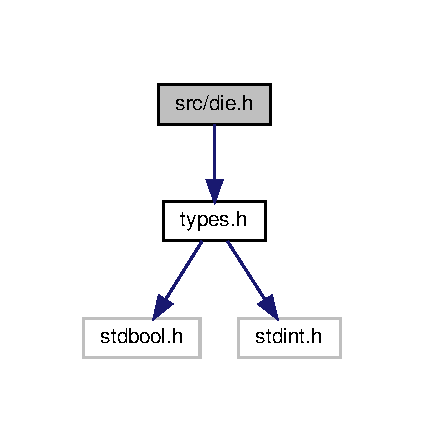
\includegraphics[width=204pt]{die_8h__incl}
\end{center}
\end{figure}
This graph shows which files directly or indirectly include this file\+:
\nopagebreak
\begin{figure}[H]
\begin{center}
\leavevmode
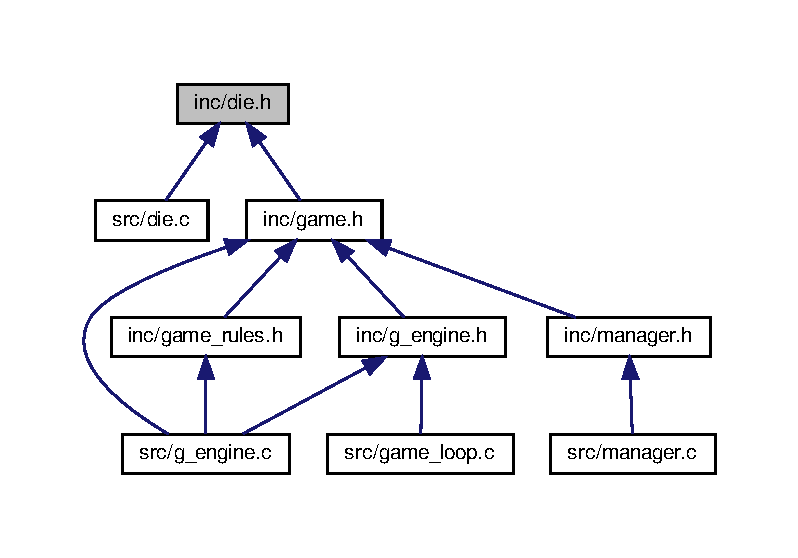
\includegraphics[width=350pt]{die_8h__dep__incl}
\end{center}
\end{figure}
\subsection*{Typedefs}
\begin{DoxyCompactItemize}
\item 
\mbox{\Hypertarget{die_8h_a892f0b0bf81d69a1f7a14ea238e36dd3}\label{die_8h_a892f0b0bf81d69a1f7a14ea238e36dd3}} 
typedef struct \hyperlink{struct__Die}{\+\_\+\+Die} {\bfseries Die}
\end{DoxyCompactItemize}
\subsection*{Functions}
\begin{DoxyCompactItemize}
\item 
\hyperlink{struct__Die}{Die} $\ast$ \hyperlink{die_8h_a47b145c5793416cbb7adbe4e09cff3f7}{die\+\_\+init} (\hyperlink{types_8h_a845e604fb28f7e3d97549da3448149d3}{Id} id)
\begin{DoxyCompactList}\small\item\em Initializates a die. \end{DoxyCompactList}\item 
void \hyperlink{die_8h_a0155d7ec003966bace47f3e032a368e8}{die\+\_\+destroy} (\hyperlink{struct__Die}{Die} $\ast$die)
\begin{DoxyCompactList}\small\item\em destroys a die \end{DoxyCompactList}\item 
int \hyperlink{die_8h_a06289514edbedf660c4b043f78e859fc}{die\+\_\+roll} (\hyperlink{struct__Die}{Die} $\ast$die)
\begin{DoxyCompactList}\small\item\em rolls a die getting a random number \end{DoxyCompactList}\item 
const int \hyperlink{die_8h_a0ae47c02f343ffdbdf0750bb4864558b}{die\+\_\+get\+\_\+lastn} (\hyperlink{struct__Die}{Die} $\ast$die)
\begin{DoxyCompactList}\small\item\em gets the last random number of the die \end{DoxyCompactList}\end{DoxyCompactItemize}


\subsection{Detailed Description}
Die\textquotesingle{}s module header. 

\begin{DoxyVersion}{Version}
0.\+0.\+3 
\end{DoxyVersion}
\begin{DoxyDate}{Date}
10/03/2019 
\end{DoxyDate}
\begin{DoxyAuthor}{Author}
Javier Romera 
\end{DoxyAuthor}
\begin{DoxyCopyright}{Copyright}
G\+NU Public License 
\end{DoxyCopyright}


\subsection{Function Documentation}
\mbox{\Hypertarget{die_8h_a47b145c5793416cbb7adbe4e09cff3f7}\label{die_8h_a47b145c5793416cbb7adbe4e09cff3f7}} 
\index{die.\+h@{die.\+h}!die\+\_\+init@{die\+\_\+init}}
\index{die\+\_\+init@{die\+\_\+init}!die.\+h@{die.\+h}}
\subsubsection{\texorpdfstring{die\+\_\+init()}{die\_init()}}
{\footnotesize\ttfamily \hyperlink{struct__Die}{Die}$\ast$ die\+\_\+init (\begin{DoxyParamCaption}\item[{\hyperlink{types_8h_a845e604fb28f7e3d97549da3448149d3}{Id}}]{id }\end{DoxyParamCaption})}



Initializates a die. 

\begin{DoxyAuthor}{Author}
Javier Romera 
\end{DoxyAuthor}

\begin{DoxyParams}{Parameters}
{\em \{\+Id\}} & id -\/ Die identification \\
\hline
\end{DoxyParams}

\begin{DoxyRetVals}{Return values}
{\em Returns} & a pointer towards die \\
\hline
\end{DoxyRetVals}
\mbox{\Hypertarget{die_8h_a0155d7ec003966bace47f3e032a368e8}\label{die_8h_a0155d7ec003966bace47f3e032a368e8}} 
\index{die.\+h@{die.\+h}!die\+\_\+destroy@{die\+\_\+destroy}}
\index{die\+\_\+destroy@{die\+\_\+destroy}!die.\+h@{die.\+h}}
\subsubsection{\texorpdfstring{die\+\_\+destroy()}{die\_destroy()}}
{\footnotesize\ttfamily void die\+\_\+destroy (\begin{DoxyParamCaption}\item[{\hyperlink{struct__Die}{Die} $\ast$}]{die }\end{DoxyParamCaption})}



destroys a die 

\begin{DoxyAuthor}{Author}
Javier Romera 
\end{DoxyAuthor}

\begin{DoxyParams}{Parameters}
{\em \{\+Die$\ast$\}} & die -\/ Die pointer \\
\hline
\end{DoxyParams}
\mbox{\Hypertarget{die_8h_a06289514edbedf660c4b043f78e859fc}\label{die_8h_a06289514edbedf660c4b043f78e859fc}} 
\index{die.\+h@{die.\+h}!die\+\_\+roll@{die\+\_\+roll}}
\index{die\+\_\+roll@{die\+\_\+roll}!die.\+h@{die.\+h}}
\subsubsection{\texorpdfstring{die\+\_\+roll()}{die\_roll()}}
{\footnotesize\ttfamily int die\+\_\+roll (\begin{DoxyParamCaption}\item[{\hyperlink{struct__Die}{Die} $\ast$}]{die }\end{DoxyParamCaption})}



rolls a die getting a random number 

\begin{DoxyAuthor}{Author}
Javier Romera 
\end{DoxyAuthor}

\begin{DoxyParams}{Parameters}
{\em \{\+Die$\ast$\}} & die -\/ Die pointer \\
\hline
\end{DoxyParams}

\begin{DoxyRetVals}{Return values}
{\em \{int\}} & -\/ Returns the random number; \\
\hline
\end{DoxyRetVals}
\mbox{\Hypertarget{die_8h_a0ae47c02f343ffdbdf0750bb4864558b}\label{die_8h_a0ae47c02f343ffdbdf0750bb4864558b}} 
\index{die.\+h@{die.\+h}!die\+\_\+get\+\_\+lastn@{die\+\_\+get\+\_\+lastn}}
\index{die\+\_\+get\+\_\+lastn@{die\+\_\+get\+\_\+lastn}!die.\+h@{die.\+h}}
\subsubsection{\texorpdfstring{die\+\_\+get\+\_\+lastn()}{die\_get\_lastn()}}
{\footnotesize\ttfamily const int die\+\_\+get\+\_\+lastn (\begin{DoxyParamCaption}\item[{\hyperlink{struct__Die}{Die} $\ast$}]{die }\end{DoxyParamCaption})}



gets the last random number of the die 

\begin{DoxyAuthor}{Author}
Javier Romera 
\end{DoxyAuthor}

\begin{DoxyParams}{Parameters}
{\em \{\+Die$\ast$\}} & die -\/ Die pointer \\
\hline
\end{DoxyParams}

\begin{DoxyRetVals}{Return values}
{\em \{int\}} & -\/ Returns the last random number; \\
\hline
\end{DoxyRetVals}

\hypertarget{g__engine_8h}{}\section{inc/g\+\_\+engine.h File Reference}
\label{g__engine_8h}\index{inc/g\+\_\+engine.\+h@{inc/g\+\_\+engine.\+h}}


Main graphic engine.  


{\ttfamily \#include \char`\"{}game.\+h\char`\"{}}\newline
Include dependency graph for g\+\_\+engine.\+h\+:\nopagebreak
\begin{figure}[H]
\begin{center}
\leavevmode
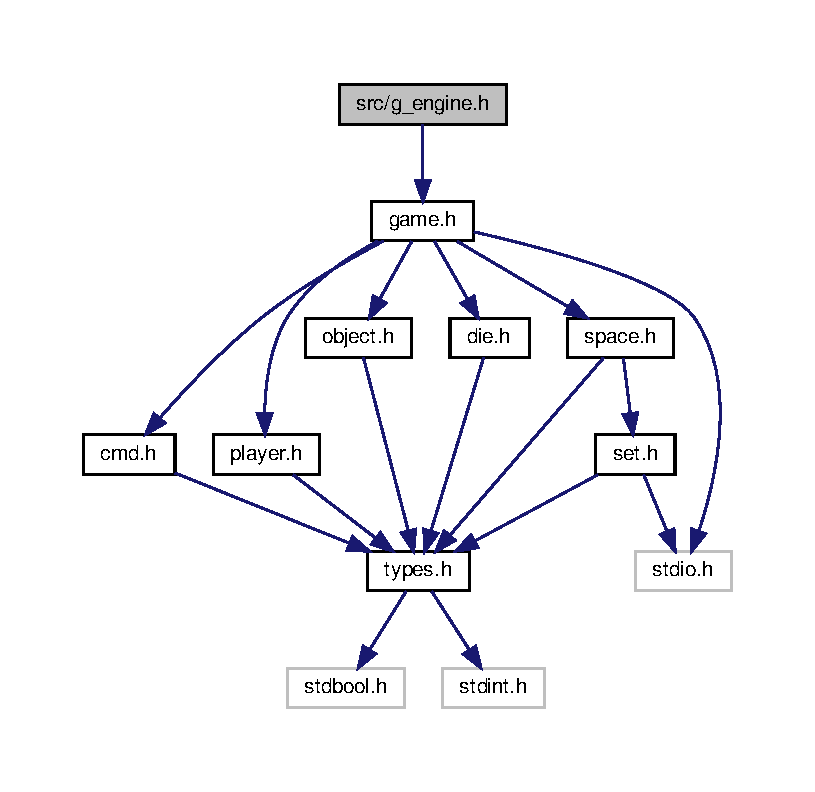
\includegraphics[width=350pt]{g__engine_8h__incl}
\end{center}
\end{figure}
This graph shows which files directly or indirectly include this file\+:\nopagebreak
\begin{figure}[H]
\begin{center}
\leavevmode
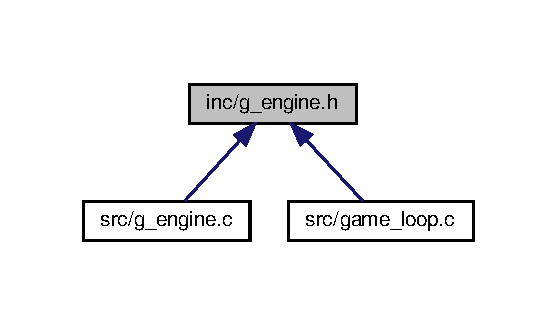
\includegraphics[width=268pt]{g__engine_8h__dep__incl}
\end{center}
\end{figure}
\subsection*{Typedefs}
\begin{DoxyCompactItemize}
\item 
\mbox{\Hypertarget{g__engine_8h_a89d836c348f7c2eb5b9b42d64a093eaa}\label{g__engine_8h_a89d836c348f7c2eb5b9b42d64a093eaa}} 
typedef struct \hyperlink{struct__G__engine}{\+\_\+\+G\+\_\+engine} {\bfseries G\+\_\+engine}
\end{DoxyCompactItemize}
\subsection*{Functions}
\begin{DoxyCompactItemize}
\item 
\hyperlink{struct__G__engine}{G\+\_\+engine} $\ast$ \hyperlink{g__engine_8h_aa2f5a0548ea6fedb671c594d4f0cf039}{g\+\_\+engine\+\_\+create} ()
\begin{DoxyCompactList}\small\item\em Creates a new graphic engine. \end{DoxyCompactList}\item 
void \hyperlink{g__engine_8h_ae61d1ed693a2bfc2967b4550fc128536}{g\+\_\+engine\+\_\+destroy} (\hyperlink{struct__G__engine}{G\+\_\+engine} $\ast$ge)
\begin{DoxyCompactList}\small\item\em Destroys a graphic engine. \end{DoxyCompactList}\item 
void \hyperlink{g__engine_8h_a22856c5bd4a0185424313f9fcb5ed4d7}{g\+\_\+engine\+\_\+paint\+\_\+help} (\hyperlink{struct__G__engine}{G\+\_\+engine} $\ast$ge, \hyperlink{struct__Game}{Game} $\ast$game)
\begin{DoxyCompactList}\small\item\em Draws the help interface. \end{DoxyCompactList}\item 
void \hyperlink{g__engine_8h_ab215509a5b24333ada8465e80df43387}{g\+\_\+engine\+\_\+paint\+\_\+game} (\hyperlink{struct__G__engine}{G\+\_\+engine} $\ast$ge, \hyperlink{struct__Game}{Game} $\ast$game)
\begin{DoxyCompactList}\small\item\em Draws the game interface. \end{DoxyCompactList}\end{DoxyCompactItemize}


\subsection{Detailed Description}
Main graphic engine. 

\begin{DoxyVersion}{Version}
0.\+7.\+1 
\end{DoxyVersion}
\begin{DoxyDate}{Date}
10/03/2019 
\end{DoxyDate}
\begin{DoxyCopyright}{Copyright}
G\+NU Public License 
\end{DoxyCopyright}


\subsection{Function Documentation}
\mbox{\Hypertarget{g__engine_8h_aa2f5a0548ea6fedb671c594d4f0cf039}\label{g__engine_8h_aa2f5a0548ea6fedb671c594d4f0cf039}} 
\index{g\+\_\+engine.\+h@{g\+\_\+engine.\+h}!g\+\_\+engine\+\_\+create@{g\+\_\+engine\+\_\+create}}
\index{g\+\_\+engine\+\_\+create@{g\+\_\+engine\+\_\+create}!g\+\_\+engine.\+h@{g\+\_\+engine.\+h}}
\subsubsection{\texorpdfstring{g\+\_\+engine\+\_\+create()}{g\_engine\_create()}}
{\footnotesize\ttfamily \hyperlink{struct__G__engine}{G\+\_\+engine}$\ast$ g\+\_\+engine\+\_\+create (\begin{DoxyParamCaption}{ }\end{DoxyParamCaption})}



Creates a new graphic engine. 


\begin{DoxyRetVals}{Return values}
{\em \{\+G\+\_\+engine$\ast$\}} & -\/ Returns a graphic engine pointer \\
\hline
\end{DoxyRetVals}
\mbox{\Hypertarget{g__engine_8h_ae61d1ed693a2bfc2967b4550fc128536}\label{g__engine_8h_ae61d1ed693a2bfc2967b4550fc128536}} 
\index{g\+\_\+engine.\+h@{g\+\_\+engine.\+h}!g\+\_\+engine\+\_\+destroy@{g\+\_\+engine\+\_\+destroy}}
\index{g\+\_\+engine\+\_\+destroy@{g\+\_\+engine\+\_\+destroy}!g\+\_\+engine.\+h@{g\+\_\+engine.\+h}}
\subsubsection{\texorpdfstring{g\+\_\+engine\+\_\+destroy()}{g\_engine\_destroy()}}
{\footnotesize\ttfamily void g\+\_\+engine\+\_\+destroy (\begin{DoxyParamCaption}\item[{\hyperlink{struct__G__engine}{G\+\_\+engine} $\ast$}]{ge }\end{DoxyParamCaption})}



Destroys a graphic engine. 


\begin{DoxyParams}{Parameters}
{\em \{\+G\+\_\+engine$\ast$\}} & ge -\/ Graphic engine pointer \\
\hline
\end{DoxyParams}
\mbox{\Hypertarget{g__engine_8h_a22856c5bd4a0185424313f9fcb5ed4d7}\label{g__engine_8h_a22856c5bd4a0185424313f9fcb5ed4d7}} 
\index{g\+\_\+engine.\+h@{g\+\_\+engine.\+h}!g\+\_\+engine\+\_\+paint\+\_\+help@{g\+\_\+engine\+\_\+paint\+\_\+help}}
\index{g\+\_\+engine\+\_\+paint\+\_\+help@{g\+\_\+engine\+\_\+paint\+\_\+help}!g\+\_\+engine.\+h@{g\+\_\+engine.\+h}}
\subsubsection{\texorpdfstring{g\+\_\+engine\+\_\+paint\+\_\+help()}{g\_engine\_paint\_help()}}
{\footnotesize\ttfamily void g\+\_\+engine\+\_\+paint\+\_\+help (\begin{DoxyParamCaption}\item[{\hyperlink{struct__G__engine}{G\+\_\+engine} $\ast$}]{ge,  }\item[{\hyperlink{struct__Game}{Game} $\ast$}]{game }\end{DoxyParamCaption})}



Draws the help interface. 


\begin{DoxyParams}{Parameters}
{\em \{\+G\+\_\+engine$\ast$\}} & ge -\/ Graphic engine pointer \\
\hline
{\em \{\+Game$\ast$\}} & game -\/ Game pointer \\
\hline
\end{DoxyParams}
\mbox{\Hypertarget{g__engine_8h_ab215509a5b24333ada8465e80df43387}\label{g__engine_8h_ab215509a5b24333ada8465e80df43387}} 
\index{g\+\_\+engine.\+h@{g\+\_\+engine.\+h}!g\+\_\+engine\+\_\+paint\+\_\+game@{g\+\_\+engine\+\_\+paint\+\_\+game}}
\index{g\+\_\+engine\+\_\+paint\+\_\+game@{g\+\_\+engine\+\_\+paint\+\_\+game}!g\+\_\+engine.\+h@{g\+\_\+engine.\+h}}
\subsubsection{\texorpdfstring{g\+\_\+engine\+\_\+paint\+\_\+game()}{g\_engine\_paint\_game()}}
{\footnotesize\ttfamily void g\+\_\+engine\+\_\+paint\+\_\+game (\begin{DoxyParamCaption}\item[{\hyperlink{struct__G__engine}{G\+\_\+engine} $\ast$}]{ge,  }\item[{\hyperlink{struct__Game}{Game} $\ast$}]{game }\end{DoxyParamCaption})}



Draws the game interface. 


\begin{DoxyParams}{Parameters}
{\em \{\+G\+\_\+engine$\ast$\}} & ge -\/ Graphic engine pointer \\
\hline
{\em \{\+Game$\ast$\}} & game -\/ Game pointer \\
\hline
\end{DoxyParams}

\hypertarget{game_8h}{}\section{inc/game.h File Reference}
\label{game_8h}\index{inc/game.\+h@{inc/game.\+h}}


It defines the game interface.  


{\ttfamily \#include \char`\"{}cmd.\+h\char`\"{}}\newline
{\ttfamily \#include \char`\"{}space.\+h\char`\"{}}\newline
{\ttfamily \#include \char`\"{}player.\+h\char`\"{}}\newline
{\ttfamily \#include \char`\"{}object.\+h\char`\"{}}\newline
{\ttfamily \#include \char`\"{}die.\+h\char`\"{}}\newline
{\ttfamily \#include \char`\"{}link.\+h\char`\"{}}\newline
{\ttfamily \#include $<$stdio.\+h$>$}\newline
Include dependency graph for game.\+h\+:\nopagebreak
\begin{figure}[H]
\begin{center}
\leavevmode
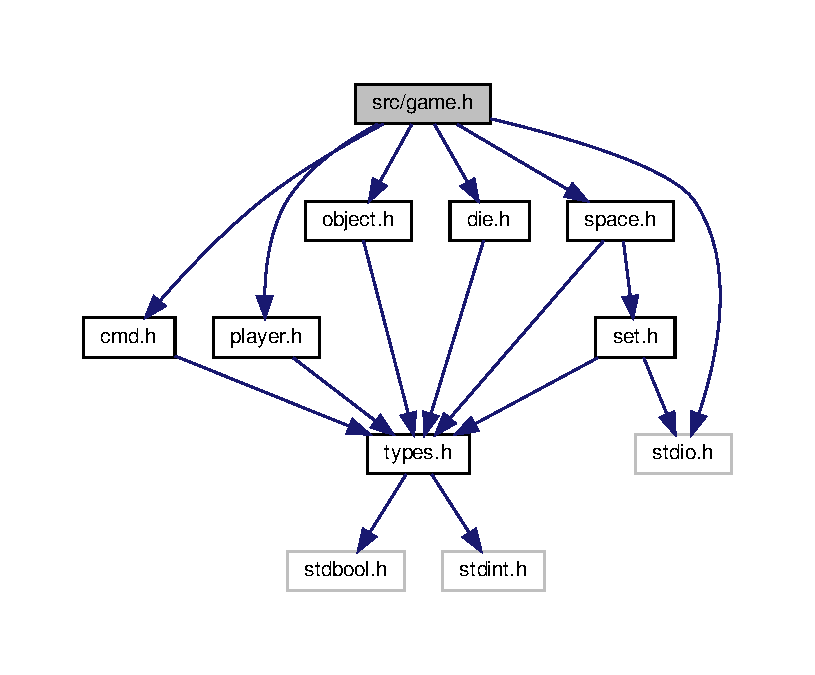
\includegraphics[width=350pt]{game_8h__incl}
\end{center}
\end{figure}
This graph shows which files directly or indirectly include this file\+:\nopagebreak
\begin{figure}[H]
\begin{center}
\leavevmode
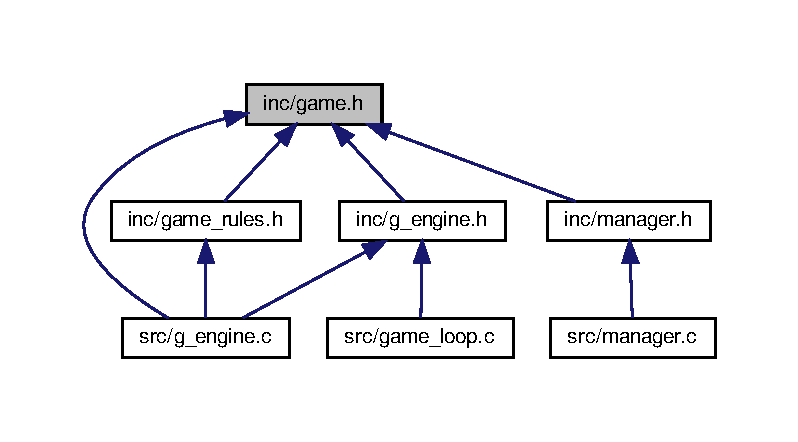
\includegraphics[width=350pt]{game_8h__dep__incl}
\end{center}
\end{figure}
\subsection*{Macros}
\begin{DoxyCompactItemize}
\item 
\mbox{\Hypertarget{game_8h_aa294c02e40f3ec02855171029ceb7d13}\label{game_8h_aa294c02e40f3ec02855171029ceb7d13}} 
\#define \hyperlink{game_8h_aa294c02e40f3ec02855171029ceb7d13}{M\+I\+N\+\_\+\+W\+I\+N\+\_\+\+C\+O\+LS}~80
\begin{DoxyCompactList}\small\item\em Minimum width of the screen. \end{DoxyCompactList}\item 
\mbox{\Hypertarget{game_8h_abf182269072323ec4e8ef1efa10e4c7f}\label{game_8h_abf182269072323ec4e8ef1efa10e4c7f}} 
\#define \hyperlink{game_8h_abf182269072323ec4e8ef1efa10e4c7f}{M\+I\+N\+\_\+\+W\+I\+N\+\_\+\+R\+O\+WS}~24
\begin{DoxyCompactList}\small\item\em Minimum height of the screen. \end{DoxyCompactList}\end{DoxyCompactItemize}
\subsection*{Typedefs}
\begin{DoxyCompactItemize}
\item 
\mbox{\Hypertarget{game_8h_a57156d39c530aec3fba3a9dad8c2dc6a}\label{game_8h_a57156d39c530aec3fba3a9dad8c2dc6a}} 
typedef struct \hyperlink{struct__Game}{\+\_\+\+Game} {\bfseries Game}
\end{DoxyCompactItemize}
\subsection*{Enumerations}
\begin{DoxyCompactItemize}
\item 
\mbox{\Hypertarget{game_8h_abc6126af1d45847bc59afa0aa3216b04}\label{game_8h_abc6126af1d45847bc59afa0aa3216b04}} 
enum \{ {\bfseries G\+A\+M\+E\+\_\+\+S\+P\+A\+C\+ES}, 
{\bfseries G\+A\+M\+E\+\_\+\+L\+I\+N\+KS}, 
{\bfseries G\+A\+M\+E\+\_\+\+O\+B\+J\+E\+C\+TS}
 \}
\end{DoxyCompactItemize}
\subsection*{Functions}
\begin{DoxyCompactItemize}
\item 
\hyperlink{types_8h_a32c27cc471df37f4fc818d65de0a56c4}{S\+T\+A\+T\+US} \hyperlink{game_8h_ae5ad86de0a92d9eccb234948458da7f1}{game\+\_\+add\+\_\+space} (\hyperlink{struct__Game}{Game} $\ast$game, \hyperlink{space_8h_a67533ffc2b70463baecc38fb0629bbfc}{Space} $\ast$space)
\begin{DoxyCompactList}\small\item\em Adds a given space into the game. \end{DoxyCompactList}\item 
\hyperlink{types_8h_a32c27cc471df37f4fc818d65de0a56c4}{S\+T\+A\+T\+US} \hyperlink{game_8h_ac332bb8c230f5e1c83b43fa1ed809194}{game\+\_\+add\+\_\+link} (\hyperlink{struct__Game}{Game} $\ast$game, \hyperlink{struct__Link}{Link} $\ast$ln)
\begin{DoxyCompactList}\small\item\em Adds a given link into the game. \end{DoxyCompactList}\item 
\hyperlink{struct__Game}{Game} $\ast$ \hyperlink{game_8h_a1cdbe3f06b9bf49eb5e334a22ad3b2b9}{game\+\_\+create} ()
\begin{DoxyCompactList}\small\item\em presets game initial state onto N\+U\+LL \end{DoxyCompactList}\item 
\hyperlink{types_8h_a32c27cc471df37f4fc818d65de0a56c4}{S\+T\+A\+T\+US} \hyperlink{game_8h_aa507cc4e4968737c1b2ea85e9da0362a}{game\+\_\+load\+\_\+from\+\_\+file} (\hyperlink{struct__Game}{Game} $\ast$game, char $\ast$filename)
\begin{DoxyCompactList}\small\item\em presets game state with the data value included in the save file \end{DoxyCompactList}\item 
\hyperlink{types_8h_a32c27cc471df37f4fc818d65de0a56c4}{S\+T\+A\+T\+US} \hyperlink{game_8h_a4a8f3de1cdc4bcb9a508a191677ee33f}{game\+\_\+update} (\hyperlink{struct__Game}{Game} $\ast$game, \hyperlink{cmd_8h_ab2b68b94b84c77ba11a699a76b8cf9cc}{Cmd} $\ast$cmd)
\begin{DoxyCompactList}\small\item\em sets the last command value onto last key introduced \end{DoxyCompactList}\item 
\hyperlink{types_8h_a32c27cc471df37f4fc818d65de0a56c4}{S\+T\+A\+T\+US} \hyperlink{game_8h_a0736924a1235c0e6fe9b6d91c2a12af8}{game\+\_\+destroy} (\hyperlink{struct__Game}{Game} $\ast$game)
\begin{DoxyCompactList}\small\item\em frees dynamic memory reserved in game \end{DoxyCompactList}\item 
bool \hyperlink{game_8h_a27711fe1fc6f5a353b9ab63b92602359}{game\+\_\+is\+\_\+over} (\hyperlink{struct__Game}{Game} $\ast$game)
\begin{DoxyCompactList}\small\item\em quits game \end{DoxyCompactList}\item 
\hyperlink{space_8h_a67533ffc2b70463baecc38fb0629bbfc}{Space} $\ast$ \hyperlink{game_8h_a69d94da9d27b542d3ebdeb8b60f1f2dc}{game\+\_\+get\+\_\+space} (\hyperlink{struct__Game}{Game} $\ast$game, \hyperlink{types_8h_a845e604fb28f7e3d97549da3448149d3}{Id} id)
\begin{DoxyCompactList}\small\item\em gets all the existing spaces with the same id if the id passed as argument exist \end{DoxyCompactList}\item 
\hyperlink{space_8h_a67533ffc2b70463baecc38fb0629bbfc}{Space} $\ast$ \hyperlink{game_8h_a5c8922fd5fc6de08b0b57899013ad117}{game\+\_\+get\+\_\+object\+\_\+space} (\hyperlink{struct__Game}{Game} $\ast$game, \hyperlink{types_8h_a845e604fb28f7e3d97549da3448149d3}{Id} id)
\begin{DoxyCompactList}\small\item\em gets the space of an object \end{DoxyCompactList}\item 
\hyperlink{types_8h_a32c27cc471df37f4fc818d65de0a56c4}{S\+T\+A\+T\+US} \hyperlink{game_8h_ad361335e40fd953eaf6839414617eb5b}{game\+\_\+set\+\_\+object\+\_\+location} (\hyperlink{struct__Game}{Game} $\ast$game, \hyperlink{types_8h_a845e604fb28f7e3d97549da3448149d3}{Id} id)
\begin{DoxyCompactList}\small\item\em set the position of an object in the game \end{DoxyCompactList}\item 
\hyperlink{struct__Player}{Player} $\ast$ \hyperlink{game_8h_af46efd507d797aec6da90d08aa592e32}{game\+\_\+get\+\_\+player} (\hyperlink{struct__Game}{Game} $\ast$game)
\begin{DoxyCompactList}\small\item\em gets a pointer towards player \end{DoxyCompactList}\item 
\hyperlink{object_8h_a7f8bbcda919b65ce67f92fba08e0212f}{Object} $\ast$ \hyperlink{game_8h_a7ca2ae962cbba287a65d71efdcd4ff93}{game\+\_\+get\+\_\+object\+\_\+by\+\_\+id} (\hyperlink{struct__Game}{Game} $\ast$game, \hyperlink{types_8h_a845e604fb28f7e3d97549da3448149d3}{Id} id)
\begin{DoxyCompactList}\small\item\em gets a object by id \end{DoxyCompactList}\item 
\hyperlink{object_8h_a7f8bbcda919b65ce67f92fba08e0212f}{Object} $\ast$ \hyperlink{game_8h_aea02495378a96ed422b8bc67552d69d7}{game\+\_\+get\+\_\+object\+\_\+by\+\_\+idx} (\hyperlink{struct__Game}{Game} $\ast$game, int idx)
\begin{DoxyCompactList}\small\item\em gets a object by idx \end{DoxyCompactList}\item 
\hyperlink{object_8h_a7f8bbcda919b65ce67f92fba08e0212f}{Object} $\ast$ \hyperlink{game_8h_a1ee080f6cdfb95f72007e688927da393}{game\+\_\+get\+\_\+object\+\_\+by\+\_\+name} (\hyperlink{struct__Game}{Game} $\ast$game, const char $\ast$name)
\begin{DoxyCompactList}\small\item\em gets a object by name \end{DoxyCompactList}\item 
\hyperlink{struct__Link}{Link} $\ast$ \hyperlink{game_8h_aa06d97f52a3b567c59d511661c4c7ad0}{game\+\_\+get\+\_\+link\+\_\+by\+\_\+id} (\hyperlink{struct__Game}{Game} $\ast$game, \hyperlink{types_8h_a845e604fb28f7e3d97549da3448149d3}{Id} id)
\begin{DoxyCompactList}\small\item\em Gets a link by it\textquotesingle{}s id. \end{DoxyCompactList}\item 
\hyperlink{types_8h_a32c27cc471df37f4fc818d65de0a56c4}{S\+T\+A\+T\+US} \hyperlink{game_8h_ade0d25f267771b1f9b27fcc0383e93b8}{game\+\_\+set\+\_\+player} (\hyperlink{struct__Game}{Game} $\ast$game, \hyperlink{struct__Player}{Player} $\ast$player)
\begin{DoxyCompactList}\small\item\em sets a new player \end{DoxyCompactList}\item 
\hyperlink{types_8h_a32c27cc471df37f4fc818d65de0a56c4}{S\+T\+A\+T\+US} \hyperlink{game_8h_a9597a8e456aa74db536e87d56f56c3b4}{game\+\_\+add\+\_\+object} (\hyperlink{struct__Game}{Game} $\ast$game, \hyperlink{object_8h_a7f8bbcda919b65ce67f92fba08e0212f}{Object} $\ast$object)
\begin{DoxyCompactList}\small\item\em sets a new object \end{DoxyCompactList}\item 
void \hyperlink{game_8h_a9d64221dbc653f866adc43c4ef849bb1}{game\+\_\+set\+\_\+die} (\hyperlink{struct__Game}{Game} $\ast$game, \hyperlink{struct__Die}{Die} $\ast$d)
\begin{DoxyCompactList}\small\item\em sets a new die \end{DoxyCompactList}\item 
\hyperlink{space_8h_a67533ffc2b70463baecc38fb0629bbfc}{Space} $\ast$ \hyperlink{game_8h_ab2506331340cbef8592780e0564cc8b7}{game\+\_\+get\+\_\+last\+\_\+space} (\hyperlink{struct__Game}{Game} $\ast$game)
\begin{DoxyCompactList}\small\item\em gets a pointer towards last space \end{DoxyCompactList}\item 
\mbox{\Hypertarget{game_8h_ac43df8654f7e438bca33449c0de67aa7}\label{game_8h_ac43df8654f7e438bca33449c0de67aa7}} 
void {\bfseries game\+\_\+get\+\_\+spaces} (\hyperlink{struct__Game}{Game} $\ast$game, int max, \hyperlink{space_8h_a67533ffc2b70463baecc38fb0629bbfc}{Space} $\ast$$\ast$spaces, int $\ast$total)
\item 
\mbox{\Hypertarget{game_8h_a00ec1903ad0212873b64668de5984f0d}\label{game_8h_a00ec1903ad0212873b64668de5984f0d}} 
void {\bfseries game\+\_\+get\+\_\+links} (\hyperlink{struct__Game}{Game} $\ast$game, int max, \hyperlink{struct__Link}{Link} $\ast$$\ast$links, int $\ast$total)
\item 
\mbox{\Hypertarget{game_8h_a59eac3fe8bb037c712ca0957b798cf72}\label{game_8h_a59eac3fe8bb037c712ca0957b798cf72}} 
void {\bfseries game\+\_\+get\+\_\+objects} (\hyperlink{struct__Game}{Game} $\ast$game, int max, \hyperlink{object_8h_a7f8bbcda919b65ce67f92fba08e0212f}{Object} $\ast$$\ast$objs, int $\ast$total)
\item 
\hyperlink{space_8h_a67533ffc2b70463baecc38fb0629bbfc}{Space} $\ast$ \hyperlink{game_8h_a584f1f96a3b7b428d7a6d76aa26dff2c}{game\+\_\+get\+\_\+first\+\_\+space} (\hyperlink{struct__Game}{Game} $\ast$game)
\begin{DoxyCompactList}\small\item\em gets a pointer towards first space \end{DoxyCompactList}\item 
\hyperlink{struct__Die}{Die} $\ast$ \hyperlink{game_8h_a5753a09313b092a52c0cea742c40f3cf}{game\+\_\+get\+\_\+die} (\hyperlink{struct__Game}{Game} $\ast$game)
\begin{DoxyCompactList}\small\item\em gets a pointer towards die \end{DoxyCompactList}\item 
\hyperlink{cmd_8h_ab2b68b94b84c77ba11a699a76b8cf9cc}{Cmd} $\ast$ \hyperlink{game_8h_ad4f3192f7515879d7ff47522a7f489d7}{game\+\_\+get\+\_\+cmd} (\hyperlink{struct__Game}{Game} $\ast$game)
\begin{DoxyCompactList}\small\item\em gets a pointer towards cmd \end{DoxyCompactList}\item 
\mbox{\Hypertarget{game_8h_a63b8fadde2c72953a6264d972bbf9871}\label{game_8h_a63b8fadde2c72953a6264d972bbf9871}} 
\hyperlink{types_8h_a32c27cc471df37f4fc818d65de0a56c4}{S\+T\+A\+T\+US} {\bfseries game\+\_\+clean} (\hyperlink{struct__Game}{Game} $\ast$game)
\end{DoxyCompactItemize}


\subsection{Detailed Description}
It defines the game interface. 

\begin{DoxyVersion}{Version}
0.\+5.\+1 
\end{DoxyVersion}
\begin{DoxyDate}{Date}
14/03/2019 
\end{DoxyDate}
\begin{DoxyCopyright}{Copyright}
G\+NU Public License 
\end{DoxyCopyright}


\subsection{Function Documentation}
\mbox{\Hypertarget{game_8h_ae5ad86de0a92d9eccb234948458da7f1}\label{game_8h_ae5ad86de0a92d9eccb234948458da7f1}} 
\index{game.\+h@{game.\+h}!game\+\_\+add\+\_\+space@{game\+\_\+add\+\_\+space}}
\index{game\+\_\+add\+\_\+space@{game\+\_\+add\+\_\+space}!game.\+h@{game.\+h}}
\subsubsection{\texorpdfstring{game\+\_\+add\+\_\+space()}{game\_add\_space()}}
{\footnotesize\ttfamily \hyperlink{types_8h_a32c27cc471df37f4fc818d65de0a56c4}{S\+T\+A\+T\+US} game\+\_\+add\+\_\+space (\begin{DoxyParamCaption}\item[{\hyperlink{struct__Game}{Game} $\ast$}]{game,  }\item[{\hyperlink{space_8h_a67533ffc2b70463baecc38fb0629bbfc}{Space} $\ast$}]{space }\end{DoxyParamCaption})}



Adds a given space into the game. 


\begin{DoxyParams}{Parameters}
{\em \{\+Game$\ast$\}} & game -\/ Game pointer \\
\hline
{\em \{\+Space$\ast$\}} & space -\/ Space pointer \\
\hline
\end{DoxyParams}

\begin{DoxyRetVals}{Return values}
{\em \{\+S\+T\+A\+T\+U\+S\}} & -\/ Returns an status code \\
\hline
\end{DoxyRetVals}
\mbox{\Hypertarget{game_8h_ac332bb8c230f5e1c83b43fa1ed809194}\label{game_8h_ac332bb8c230f5e1c83b43fa1ed809194}} 
\index{game.\+h@{game.\+h}!game\+\_\+add\+\_\+link@{game\+\_\+add\+\_\+link}}
\index{game\+\_\+add\+\_\+link@{game\+\_\+add\+\_\+link}!game.\+h@{game.\+h}}
\subsubsection{\texorpdfstring{game\+\_\+add\+\_\+link()}{game\_add\_link()}}
{\footnotesize\ttfamily \hyperlink{types_8h_a32c27cc471df37f4fc818d65de0a56c4}{S\+T\+A\+T\+US} game\+\_\+add\+\_\+link (\begin{DoxyParamCaption}\item[{\hyperlink{struct__Game}{Game} $\ast$}]{game,  }\item[{\hyperlink{struct__Link}{Link} $\ast$}]{ln }\end{DoxyParamCaption})}



Adds a given link into the game. 


\begin{DoxyParams}{Parameters}
{\em \{\+Game$\ast$\}} & game -\/ Game where the link should be added \\
\hline
{\em \{\+Space$\ast$\}} & ln -\/ Link to be added \\
\hline
\end{DoxyParams}

\begin{DoxyRetVals}{Return values}
{\em \{\+S\+T\+A\+T\+U\+S\}} & -\/ Returns an status code \\
\hline
\end{DoxyRetVals}
\mbox{\Hypertarget{game_8h_a1cdbe3f06b9bf49eb5e334a22ad3b2b9}\label{game_8h_a1cdbe3f06b9bf49eb5e334a22ad3b2b9}} 
\index{game.\+h@{game.\+h}!game\+\_\+create@{game\+\_\+create}}
\index{game\+\_\+create@{game\+\_\+create}!game.\+h@{game.\+h}}
\subsubsection{\texorpdfstring{game\+\_\+create()}{game\_create()}}
{\footnotesize\ttfamily \hyperlink{struct__Game}{Game}$\ast$ game\+\_\+create (\begin{DoxyParamCaption}{ }\end{DoxyParamCaption})}



presets game initial state onto N\+U\+LL 

\begin{DoxyAuthor}{Author}
Javier Romera 
\end{DoxyAuthor}

\begin{DoxyParams}{Parameters}
{\em \{\+Game$\ast$\}} & -\/ game \\
\hline
\end{DoxyParams}

\begin{DoxyRetVals}{Return values}
{\em \{\+Game$\ast$\}} & -\/ Returns a game pointer \\
\hline
\end{DoxyRetVals}
\mbox{\Hypertarget{game_8h_aa507cc4e4968737c1b2ea85e9da0362a}\label{game_8h_aa507cc4e4968737c1b2ea85e9da0362a}} 
\index{game.\+h@{game.\+h}!game\+\_\+load\+\_\+from\+\_\+file@{game\+\_\+load\+\_\+from\+\_\+file}}
\index{game\+\_\+load\+\_\+from\+\_\+file@{game\+\_\+load\+\_\+from\+\_\+file}!game.\+h@{game.\+h}}
\subsubsection{\texorpdfstring{game\+\_\+load\+\_\+from\+\_\+file()}{game\_load\_from\_file()}}
{\footnotesize\ttfamily \hyperlink{types_8h_a32c27cc471df37f4fc818d65de0a56c4}{S\+T\+A\+T\+US} game\+\_\+load\+\_\+from\+\_\+file (\begin{DoxyParamCaption}\item[{\hyperlink{struct__Game}{Game} $\ast$}]{game,  }\item[{char $\ast$}]{filename }\end{DoxyParamCaption})}



presets game state with the data value included in the save file 

\begin{DoxyAuthor}{Author}
Álvaro Rodríguez 
\end{DoxyAuthor}

\begin{DoxyParams}{Parameters}
{\em \{\+Game$\ast$\}} & -\/ game \\
\hline
{\em \{char$\ast$\}} & -\/ filename \\
\hline
\end{DoxyParams}

\begin{DoxyRetVals}{Return values}
{\em \{\+S\+T\+A\+T\+U\+S\}} & -\/ Returns an status code \\
\hline
\end{DoxyRetVals}
\mbox{\Hypertarget{game_8h_a4a8f3de1cdc4bcb9a508a191677ee33f}\label{game_8h_a4a8f3de1cdc4bcb9a508a191677ee33f}} 
\index{game.\+h@{game.\+h}!game\+\_\+update@{game\+\_\+update}}
\index{game\+\_\+update@{game\+\_\+update}!game.\+h@{game.\+h}}
\subsubsection{\texorpdfstring{game\+\_\+update()}{game\_update()}}
{\footnotesize\ttfamily \hyperlink{types_8h_a32c27cc471df37f4fc818d65de0a56c4}{S\+T\+A\+T\+US} game\+\_\+update (\begin{DoxyParamCaption}\item[{\hyperlink{struct__Game}{Game} $\ast$}]{game,  }\item[{\hyperlink{cmd_8h_ab2b68b94b84c77ba11a699a76b8cf9cc}{Cmd} $\ast$}]{cmd }\end{DoxyParamCaption})}



sets the last command value onto last key introduced 

\begin{DoxyAuthor}{Author}
Javier Romera 
\end{DoxyAuthor}

\begin{DoxyParams}{Parameters}
{\em \{\+Game$\ast$\}} & -\/ game \\
\hline
{\em \{\+Cmd$\ast$\}} & -\/ cmd \\
\hline
\end{DoxyParams}

\begin{DoxyRetVals}{Return values}
{\em \{\+S\+T\+A\+T\+U\+S\}} & -\/ Returns an status code \\
\hline
\end{DoxyRetVals}
\mbox{\Hypertarget{game_8h_a0736924a1235c0e6fe9b6d91c2a12af8}\label{game_8h_a0736924a1235c0e6fe9b6d91c2a12af8}} 
\index{game.\+h@{game.\+h}!game\+\_\+destroy@{game\+\_\+destroy}}
\index{game\+\_\+destroy@{game\+\_\+destroy}!game.\+h@{game.\+h}}
\subsubsection{\texorpdfstring{game\+\_\+destroy()}{game\_destroy()}}
{\footnotesize\ttfamily \hyperlink{types_8h_a32c27cc471df37f4fc818d65de0a56c4}{S\+T\+A\+T\+US} game\+\_\+destroy (\begin{DoxyParamCaption}\item[{\hyperlink{struct__Game}{Game} $\ast$}]{game }\end{DoxyParamCaption})}



frees dynamic memory reserved in game 

\begin{DoxyAuthor}{Author}
Álvaro Rodríguez 
\end{DoxyAuthor}

\begin{DoxyParams}{Parameters}
{\em \{\+Game$\ast$\}} & -\/ game \\
\hline
\end{DoxyParams}

\begin{DoxyRetVals}{Return values}
{\em \{\+S\+T\+A\+T\+U\+S\}} & -\/ Returns an status code \\
\hline
\end{DoxyRetVals}
\mbox{\Hypertarget{game_8h_a27711fe1fc6f5a353b9ab63b92602359}\label{game_8h_a27711fe1fc6f5a353b9ab63b92602359}} 
\index{game.\+h@{game.\+h}!game\+\_\+is\+\_\+over@{game\+\_\+is\+\_\+over}}
\index{game\+\_\+is\+\_\+over@{game\+\_\+is\+\_\+over}!game.\+h@{game.\+h}}
\subsubsection{\texorpdfstring{game\+\_\+is\+\_\+over()}{game\_is\_over()}}
{\footnotesize\ttfamily bool game\+\_\+is\+\_\+over (\begin{DoxyParamCaption}\item[{\hyperlink{struct__Game}{Game} $\ast$}]{game }\end{DoxyParamCaption})}



quits game 

\begin{DoxyAuthor}{Author}
Javier Romera 
\end{DoxyAuthor}

\begin{DoxyParams}{Parameters}
{\em \{\+Game$\ast$\}} & -\/ game \\
\hline
\end{DoxyParams}

\begin{DoxyRetVals}{Return values}
{\em \{bool\}} & -\/ Returns a boolean value \\
\hline
\end{DoxyRetVals}
\mbox{\Hypertarget{game_8h_a69d94da9d27b542d3ebdeb8b60f1f2dc}\label{game_8h_a69d94da9d27b542d3ebdeb8b60f1f2dc}} 
\index{game.\+h@{game.\+h}!game\+\_\+get\+\_\+space@{game\+\_\+get\+\_\+space}}
\index{game\+\_\+get\+\_\+space@{game\+\_\+get\+\_\+space}!game.\+h@{game.\+h}}
\subsubsection{\texorpdfstring{game\+\_\+get\+\_\+space()}{game\_get\_space()}}
{\footnotesize\ttfamily \hyperlink{space_8h_a67533ffc2b70463baecc38fb0629bbfc}{Space}$\ast$ game\+\_\+get\+\_\+space (\begin{DoxyParamCaption}\item[{\hyperlink{struct__Game}{Game} $\ast$}]{game,  }\item[{\hyperlink{types_8h_a845e604fb28f7e3d97549da3448149d3}{Id}}]{id }\end{DoxyParamCaption})}



gets all the existing spaces with the same id if the id passed as argument exist 

\begin{DoxyAuthor}{Author}
Álvaro Rodríguez 
\end{DoxyAuthor}

\begin{DoxyParams}{Parameters}
{\em \{\+Game$\ast$\}} & -\/ game, \{Id\} -\/ id \\
\hline
\end{DoxyParams}

\begin{DoxyRetVals}{Return values}
{\em \{\+Space$\ast$\}} & -\/ Returns a space pointer \\
\hline
\end{DoxyRetVals}
\mbox{\Hypertarget{game_8h_a5c8922fd5fc6de08b0b57899013ad117}\label{game_8h_a5c8922fd5fc6de08b0b57899013ad117}} 
\index{game.\+h@{game.\+h}!game\+\_\+get\+\_\+object\+\_\+space@{game\+\_\+get\+\_\+object\+\_\+space}}
\index{game\+\_\+get\+\_\+object\+\_\+space@{game\+\_\+get\+\_\+object\+\_\+space}!game.\+h@{game.\+h}}
\subsubsection{\texorpdfstring{game\+\_\+get\+\_\+object\+\_\+space()}{game\_get\_object\_space()}}
{\footnotesize\ttfamily \hyperlink{space_8h_a67533ffc2b70463baecc38fb0629bbfc}{Space}$\ast$ game\+\_\+get\+\_\+object\+\_\+space (\begin{DoxyParamCaption}\item[{\hyperlink{struct__Game}{Game} $\ast$}]{game,  }\item[{\hyperlink{types_8h_a845e604fb28f7e3d97549da3448149d3}{Id}}]{id }\end{DoxyParamCaption})}



gets the space of an object 

\begin{DoxyAuthor}{Author}
Javier Romera 
\end{DoxyAuthor}

\begin{DoxyParams}{Parameters}
{\em \{\+Game$\ast$\}} & -\/ game \\
\hline
\end{DoxyParams}

\begin{DoxyRetVals}{Return values}
{\em \{\+Space$\ast$\}} & -\/ Returns an space pointer \\
\hline
\end{DoxyRetVals}
\mbox{\Hypertarget{game_8h_ad361335e40fd953eaf6839414617eb5b}\label{game_8h_ad361335e40fd953eaf6839414617eb5b}} 
\index{game.\+h@{game.\+h}!game\+\_\+set\+\_\+object\+\_\+location@{game\+\_\+set\+\_\+object\+\_\+location}}
\index{game\+\_\+set\+\_\+object\+\_\+location@{game\+\_\+set\+\_\+object\+\_\+location}!game.\+h@{game.\+h}}
\subsubsection{\texorpdfstring{game\+\_\+set\+\_\+object\+\_\+location()}{game\_set\_object\_location()}}
{\footnotesize\ttfamily \hyperlink{types_8h_a32c27cc471df37f4fc818d65de0a56c4}{S\+T\+A\+T\+US} game\+\_\+set\+\_\+object\+\_\+location (\begin{DoxyParamCaption}\item[{\hyperlink{struct__Game}{Game} $\ast$}]{game,  }\item[{\hyperlink{types_8h_a845e604fb28f7e3d97549da3448149d3}{Id}}]{id }\end{DoxyParamCaption})}



set the position of an object in the game 

\begin{DoxyAuthor}{Author}
Javier Romera 
\end{DoxyAuthor}

\begin{DoxyParams}{Parameters}
{\em \{\+Game$\ast$\}} & -\/ game \\
\hline
\end{DoxyParams}

\begin{DoxyRetVals}{Return values}
{\em \{\+S\+T\+A\+T\+U\+S\}} & -\/ Returns a state \\
\hline
\end{DoxyRetVals}
\mbox{\Hypertarget{game_8h_af46efd507d797aec6da90d08aa592e32}\label{game_8h_af46efd507d797aec6da90d08aa592e32}} 
\index{game.\+h@{game.\+h}!game\+\_\+get\+\_\+player@{game\+\_\+get\+\_\+player}}
\index{game\+\_\+get\+\_\+player@{game\+\_\+get\+\_\+player}!game.\+h@{game.\+h}}
\subsubsection{\texorpdfstring{game\+\_\+get\+\_\+player()}{game\_get\_player()}}
{\footnotesize\ttfamily \hyperlink{struct__Player}{Player}$\ast$ game\+\_\+get\+\_\+player (\begin{DoxyParamCaption}\item[{\hyperlink{struct__Game}{Game} $\ast$}]{game }\end{DoxyParamCaption})}



gets a pointer towards player 

\begin{DoxyAuthor}{Author}
Álvaro Rodríguez 
\end{DoxyAuthor}

\begin{DoxyParams}{Parameters}
{\em \{\+Game$\ast$\}} & -\/ game \\
\hline
\end{DoxyParams}

\begin{DoxyRetVals}{Return values}
{\em \{\+Player$\ast$\}} & -\/ Returns a player pointer \\
\hline
\end{DoxyRetVals}
\mbox{\Hypertarget{game_8h_a7ca2ae962cbba287a65d71efdcd4ff93}\label{game_8h_a7ca2ae962cbba287a65d71efdcd4ff93}} 
\index{game.\+h@{game.\+h}!game\+\_\+get\+\_\+object\+\_\+by\+\_\+id@{game\+\_\+get\+\_\+object\+\_\+by\+\_\+id}}
\index{game\+\_\+get\+\_\+object\+\_\+by\+\_\+id@{game\+\_\+get\+\_\+object\+\_\+by\+\_\+id}!game.\+h@{game.\+h}}
\subsubsection{\texorpdfstring{game\+\_\+get\+\_\+object\+\_\+by\+\_\+id()}{game\_get\_object\_by\_id()}}
{\footnotesize\ttfamily \hyperlink{object_8h_a7f8bbcda919b65ce67f92fba08e0212f}{Object}$\ast$ game\+\_\+get\+\_\+object\+\_\+by\+\_\+id (\begin{DoxyParamCaption}\item[{\hyperlink{struct__Game}{Game} $\ast$}]{game,  }\item[{\hyperlink{types_8h_a845e604fb28f7e3d97549da3448149d3}{Id}}]{id }\end{DoxyParamCaption})}



gets a object by id 

\begin{DoxyAuthor}{Author}
Javier Romera 
\end{DoxyAuthor}

\begin{DoxyParams}{Parameters}
{\em \{\+Game$\ast$\}} & -\/ game \\
\hline
\end{DoxyParams}

\begin{DoxyRetVals}{Return values}
{\em \{\+Object$\ast$\}} & -\/ Returns a player pointer \\
\hline
\end{DoxyRetVals}
\mbox{\Hypertarget{game_8h_aea02495378a96ed422b8bc67552d69d7}\label{game_8h_aea02495378a96ed422b8bc67552d69d7}} 
\index{game.\+h@{game.\+h}!game\+\_\+get\+\_\+object\+\_\+by\+\_\+idx@{game\+\_\+get\+\_\+object\+\_\+by\+\_\+idx}}
\index{game\+\_\+get\+\_\+object\+\_\+by\+\_\+idx@{game\+\_\+get\+\_\+object\+\_\+by\+\_\+idx}!game.\+h@{game.\+h}}
\subsubsection{\texorpdfstring{game\+\_\+get\+\_\+object\+\_\+by\+\_\+idx()}{game\_get\_object\_by\_idx()}}
{\footnotesize\ttfamily \hyperlink{object_8h_a7f8bbcda919b65ce67f92fba08e0212f}{Object}$\ast$ game\+\_\+get\+\_\+object\+\_\+by\+\_\+idx (\begin{DoxyParamCaption}\item[{\hyperlink{struct__Game}{Game} $\ast$}]{game,  }\item[{int}]{idx }\end{DoxyParamCaption})}



gets a object by idx 

\begin{DoxyAuthor}{Author}
Javier Romera 
\end{DoxyAuthor}

\begin{DoxyParams}{Parameters}
{\em \{\+Game$\ast$\}} & -\/ game \\
\hline
\end{DoxyParams}

\begin{DoxyRetVals}{Return values}
{\em \{\+Object$\ast$\}} & -\/ Returns a player pointer \\
\hline
\end{DoxyRetVals}
\mbox{\Hypertarget{game_8h_a1ee080f6cdfb95f72007e688927da393}\label{game_8h_a1ee080f6cdfb95f72007e688927da393}} 
\index{game.\+h@{game.\+h}!game\+\_\+get\+\_\+object\+\_\+by\+\_\+name@{game\+\_\+get\+\_\+object\+\_\+by\+\_\+name}}
\index{game\+\_\+get\+\_\+object\+\_\+by\+\_\+name@{game\+\_\+get\+\_\+object\+\_\+by\+\_\+name}!game.\+h@{game.\+h}}
\subsubsection{\texorpdfstring{game\+\_\+get\+\_\+object\+\_\+by\+\_\+name()}{game\_get\_object\_by\_name()}}
{\footnotesize\ttfamily \hyperlink{object_8h_a7f8bbcda919b65ce67f92fba08e0212f}{Object}$\ast$ game\+\_\+get\+\_\+object\+\_\+by\+\_\+name (\begin{DoxyParamCaption}\item[{\hyperlink{struct__Game}{Game} $\ast$}]{game,  }\item[{const char $\ast$}]{name }\end{DoxyParamCaption})}



gets a object by name 

\begin{DoxyAuthor}{Author}
Javier Romera 
\end{DoxyAuthor}

\begin{DoxyParams}{Parameters}
{\em \{\+Game$\ast$\}} & -\/ game \\
\hline
{\em \{char$\ast$\}} & name -\/ The name of the object \\
\hline
\end{DoxyParams}

\begin{DoxyRetVals}{Return values}
{\em \{\+Object$\ast$\}} & -\/ Returns a player pointer \\
\hline
\end{DoxyRetVals}
\mbox{\Hypertarget{game_8h_aa06d97f52a3b567c59d511661c4c7ad0}\label{game_8h_aa06d97f52a3b567c59d511661c4c7ad0}} 
\index{game.\+h@{game.\+h}!game\+\_\+get\+\_\+link\+\_\+by\+\_\+id@{game\+\_\+get\+\_\+link\+\_\+by\+\_\+id}}
\index{game\+\_\+get\+\_\+link\+\_\+by\+\_\+id@{game\+\_\+get\+\_\+link\+\_\+by\+\_\+id}!game.\+h@{game.\+h}}
\subsubsection{\texorpdfstring{game\+\_\+get\+\_\+link\+\_\+by\+\_\+id()}{game\_get\_link\_by\_id()}}
{\footnotesize\ttfamily \hyperlink{struct__Link}{Link}$\ast$ game\+\_\+get\+\_\+link\+\_\+by\+\_\+id (\begin{DoxyParamCaption}\item[{\hyperlink{struct__Game}{Game} $\ast$}]{game,  }\item[{\hyperlink{types_8h_a845e604fb28f7e3d97549da3448149d3}{Id}}]{id }\end{DoxyParamCaption})}



Gets a link by it\textquotesingle{}s id. 

\begin{DoxyAuthor}{Author}
Javier Romera 
\end{DoxyAuthor}

\begin{DoxyParams}{Parameters}
{\em \{\+Game$\ast$\}} & -\/ game  \{Id\} id -\/ The id of the link \\
\hline
\end{DoxyParams}

\begin{DoxyRetVals}{Return values}
{\em \{\+Link$\ast$\}} & -\/ Returns a link pointe or null \\
\hline
\end{DoxyRetVals}
\mbox{\Hypertarget{game_8h_ade0d25f267771b1f9b27fcc0383e93b8}\label{game_8h_ade0d25f267771b1f9b27fcc0383e93b8}} 
\index{game.\+h@{game.\+h}!game\+\_\+set\+\_\+player@{game\+\_\+set\+\_\+player}}
\index{game\+\_\+set\+\_\+player@{game\+\_\+set\+\_\+player}!game.\+h@{game.\+h}}
\subsubsection{\texorpdfstring{game\+\_\+set\+\_\+player()}{game\_set\_player()}}
{\footnotesize\ttfamily \hyperlink{types_8h_a32c27cc471df37f4fc818d65de0a56c4}{S\+T\+A\+T\+US} game\+\_\+set\+\_\+player (\begin{DoxyParamCaption}\item[{\hyperlink{struct__Game}{Game} $\ast$}]{game,  }\item[{\hyperlink{struct__Player}{Player} $\ast$}]{player }\end{DoxyParamCaption})}



sets a new player 

\begin{DoxyAuthor}{Author}
Álvaro Rodríguez 
\end{DoxyAuthor}

\begin{DoxyParams}{Parameters}
{\em \{\+Game$\ast$\}} & -\/ game \\
\hline
{\em \{\+Player$\ast$\}} & -\/ player \\
\hline
\end{DoxyParams}

\begin{DoxyRetVals}{Return values}
{\em \{\+S\+T\+A\+T\+U\+S\}} & -\/ Returns a state \\
\hline
\end{DoxyRetVals}
\mbox{\Hypertarget{game_8h_a9597a8e456aa74db536e87d56f56c3b4}\label{game_8h_a9597a8e456aa74db536e87d56f56c3b4}} 
\index{game.\+h@{game.\+h}!game\+\_\+add\+\_\+object@{game\+\_\+add\+\_\+object}}
\index{game\+\_\+add\+\_\+object@{game\+\_\+add\+\_\+object}!game.\+h@{game.\+h}}
\subsubsection{\texorpdfstring{game\+\_\+add\+\_\+object()}{game\_add\_object()}}
{\footnotesize\ttfamily \hyperlink{types_8h_a32c27cc471df37f4fc818d65de0a56c4}{S\+T\+A\+T\+US} game\+\_\+add\+\_\+object (\begin{DoxyParamCaption}\item[{\hyperlink{struct__Game}{Game} $\ast$}]{game,  }\item[{\hyperlink{object_8h_a7f8bbcda919b65ce67f92fba08e0212f}{Object} $\ast$}]{object }\end{DoxyParamCaption})}



sets a new object 

\begin{DoxyAuthor}{Author}
Javier Romera 
\end{DoxyAuthor}

\begin{DoxyParams}{Parameters}
{\em \{\+Game$\ast$\}} & -\/ game \\
\hline
{\em \{\+Object$\ast$\}} & -\/ object \\
\hline
\end{DoxyParams}

\begin{DoxyRetVals}{Return values}
{\em \{\+S\+T\+A\+T\+U\+S\}} & -\/ Returns a state \\
\hline
\end{DoxyRetVals}
\mbox{\Hypertarget{game_8h_a9d64221dbc653f866adc43c4ef849bb1}\label{game_8h_a9d64221dbc653f866adc43c4ef849bb1}} 
\index{game.\+h@{game.\+h}!game\+\_\+set\+\_\+die@{game\+\_\+set\+\_\+die}}
\index{game\+\_\+set\+\_\+die@{game\+\_\+set\+\_\+die}!game.\+h@{game.\+h}}
\subsubsection{\texorpdfstring{game\+\_\+set\+\_\+die()}{game\_set\_die()}}
{\footnotesize\ttfamily void game\+\_\+set\+\_\+die (\begin{DoxyParamCaption}\item[{\hyperlink{struct__Game}{Game} $\ast$}]{game,  }\item[{\hyperlink{struct__Die}{Die} $\ast$}]{d }\end{DoxyParamCaption})}



sets a new die 

\begin{DoxyAuthor}{Author}
Javier Romera 
\end{DoxyAuthor}

\begin{DoxyParams}{Parameters}
{\em \{\+Game$\ast$\}} & -\/ game \\
\hline
\end{DoxyParams}
\mbox{\Hypertarget{game_8h_ab2506331340cbef8592780e0564cc8b7}\label{game_8h_ab2506331340cbef8592780e0564cc8b7}} 
\index{game.\+h@{game.\+h}!game\+\_\+get\+\_\+last\+\_\+space@{game\+\_\+get\+\_\+last\+\_\+space}}
\index{game\+\_\+get\+\_\+last\+\_\+space@{game\+\_\+get\+\_\+last\+\_\+space}!game.\+h@{game.\+h}}
\subsubsection{\texorpdfstring{game\+\_\+get\+\_\+last\+\_\+space()}{game\_get\_last\_space()}}
{\footnotesize\ttfamily \hyperlink{space_8h_a67533ffc2b70463baecc38fb0629bbfc}{Space}$\ast$ game\+\_\+get\+\_\+last\+\_\+space (\begin{DoxyParamCaption}\item[{\hyperlink{struct__Game}{Game} $\ast$}]{game }\end{DoxyParamCaption})}



gets a pointer towards last space 

\begin{DoxyAuthor}{Author}
Javier Romera 
\end{DoxyAuthor}

\begin{DoxyParams}{Parameters}
{\em \{\+Game$\ast$\}} & -\/ game \\
\hline
\end{DoxyParams}

\begin{DoxyRetVals}{Return values}
{\em \{\+Space\}} & -\/ Returns a space pointer \\
\hline
\end{DoxyRetVals}
\mbox{\Hypertarget{game_8h_a584f1f96a3b7b428d7a6d76aa26dff2c}\label{game_8h_a584f1f96a3b7b428d7a6d76aa26dff2c}} 
\index{game.\+h@{game.\+h}!game\+\_\+get\+\_\+first\+\_\+space@{game\+\_\+get\+\_\+first\+\_\+space}}
\index{game\+\_\+get\+\_\+first\+\_\+space@{game\+\_\+get\+\_\+first\+\_\+space}!game.\+h@{game.\+h}}
\subsubsection{\texorpdfstring{game\+\_\+get\+\_\+first\+\_\+space()}{game\_get\_first\_space()}}
{\footnotesize\ttfamily \hyperlink{space_8h_a67533ffc2b70463baecc38fb0629bbfc}{Space}$\ast$ game\+\_\+get\+\_\+first\+\_\+space (\begin{DoxyParamCaption}\item[{\hyperlink{struct__Game}{Game} $\ast$}]{game }\end{DoxyParamCaption})}



gets a pointer towards first space 

\begin{DoxyAuthor}{Author}
Javier Romera 
\end{DoxyAuthor}

\begin{DoxyParams}{Parameters}
{\em \{\+Game$\ast$\}} & -\/ game \\
\hline
\end{DoxyParams}

\begin{DoxyRetVals}{Return values}
{\em \{\+Space\}} & -\/ Returns a space pointer \\
\hline
\end{DoxyRetVals}
\mbox{\Hypertarget{game_8h_a5753a09313b092a52c0cea742c40f3cf}\label{game_8h_a5753a09313b092a52c0cea742c40f3cf}} 
\index{game.\+h@{game.\+h}!game\+\_\+get\+\_\+die@{game\+\_\+get\+\_\+die}}
\index{game\+\_\+get\+\_\+die@{game\+\_\+get\+\_\+die}!game.\+h@{game.\+h}}
\subsubsection{\texorpdfstring{game\+\_\+get\+\_\+die()}{game\_get\_die()}}
{\footnotesize\ttfamily \hyperlink{struct__Die}{Die}$\ast$ game\+\_\+get\+\_\+die (\begin{DoxyParamCaption}\item[{\hyperlink{struct__Game}{Game} $\ast$}]{game }\end{DoxyParamCaption})}



gets a pointer towards die 

\begin{DoxyAuthor}{Author}
Javier Romera 
\end{DoxyAuthor}

\begin{DoxyParams}{Parameters}
{\em \{\+Game$\ast$\}} & -\/ game \\
\hline
\end{DoxyParams}

\begin{DoxyRetVals}{Return values}
{\em \{\+Player\}} & -\/ Returns a die pointer \\
\hline
\end{DoxyRetVals}
\mbox{\Hypertarget{game_8h_ad4f3192f7515879d7ff47522a7f489d7}\label{game_8h_ad4f3192f7515879d7ff47522a7f489d7}} 
\index{game.\+h@{game.\+h}!game\+\_\+get\+\_\+cmd@{game\+\_\+get\+\_\+cmd}}
\index{game\+\_\+get\+\_\+cmd@{game\+\_\+get\+\_\+cmd}!game.\+h@{game.\+h}}
\subsubsection{\texorpdfstring{game\+\_\+get\+\_\+cmd()}{game\_get\_cmd()}}
{\footnotesize\ttfamily \hyperlink{cmd_8h_ab2b68b94b84c77ba11a699a76b8cf9cc}{Cmd}$\ast$ game\+\_\+get\+\_\+cmd (\begin{DoxyParamCaption}\item[{\hyperlink{struct__Game}{Game} $\ast$}]{game }\end{DoxyParamCaption})}



gets a pointer towards cmd 

\begin{DoxyAuthor}{Author}
Javier Romera 
\end{DoxyAuthor}

\begin{DoxyParams}{Parameters}
{\em \{\+Game$\ast$\}} & -\/ game \\
\hline
\end{DoxyParams}

\begin{DoxyRetVals}{Return values}
{\em \{\+Player\}} & -\/ Returns a cmd pointer \\
\hline
\end{DoxyRetVals}

\hypertarget{inventory_8h}{}\section{src/inventory.h File Reference}
\label{inventory_8h}\index{src/inventory.\+h@{src/inventory.\+h}}


Defines player\textquotesingle{}s inventory.  


{\ttfamily \#include $<$stdio.\+h$>$}\newline
{\ttfamily \#include \char`\"{}types.\+h\char`\"{}}\newline
Include dependency graph for inventory.\+h\+:\nopagebreak
\begin{figure}[H]
\begin{center}
\leavevmode
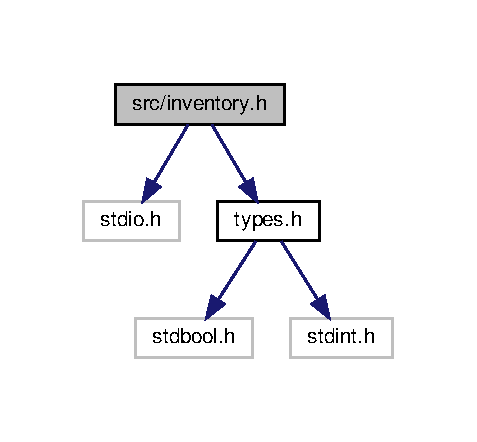
\includegraphics[width=229pt]{inventory_8h__incl}
\end{center}
\end{figure}
This graph shows which files directly or indirectly include this file\+:\nopagebreak
\begin{figure}[H]
\begin{center}
\leavevmode
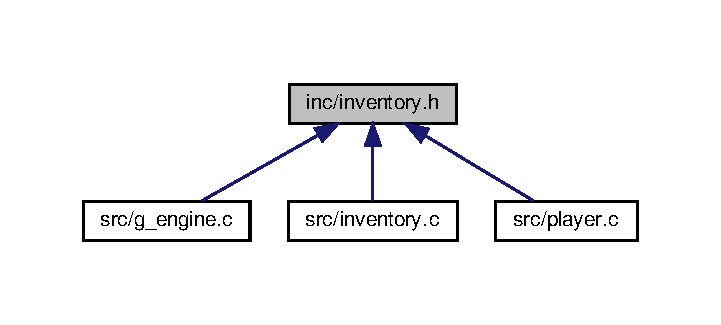
\includegraphics[width=161pt]{inventory_8h__dep__incl}
\end{center}
\end{figure}
\subsection*{Macros}
\begin{DoxyCompactItemize}
\item 
\mbox{\Hypertarget{inventory_8h_a44ebc1f23fbda13f8df116041c33c5f0}\label{inventory_8h_a44ebc1f23fbda13f8df116041c33c5f0}} 
\#define {\bfseries M\+A\+X\+\_\+\+I\+N\+V\+E\+N\+T\+O\+RY}~5
\end{DoxyCompactItemize}
\subsection*{Typedefs}
\begin{DoxyCompactItemize}
\item 
\mbox{\Hypertarget{inventory_8h_a2253bf64ac4ce6a9c1d6f39c0b0d32a3}\label{inventory_8h_a2253bf64ac4ce6a9c1d6f39c0b0d32a3}} 
typedef struct \hyperlink{struct__Inventory}{\+\_\+\+Inventory} {\bfseries Inventory}
\end{DoxyCompactItemize}
\subsection*{Functions}
\begin{DoxyCompactItemize}
\item 
\mbox{\Hypertarget{inventory_8h_a5d6b47f7a727932c56d66a65fb540910}\label{inventory_8h_a5d6b47f7a727932c56d66a65fb540910}} 
\hyperlink{struct__Inventory}{Inventory} $\ast$ {\bfseries inventory\+\_\+create} ()
\item 
\mbox{\Hypertarget{inventory_8h_a90250adb627aaa1305954287a9154966}\label{inventory_8h_a90250adb627aaa1305954287a9154966}} 
void {\bfseries inventory\+\_\+destroy} (\hyperlink{struct__Inventory}{Inventory} $\ast$inv)
\item 
\mbox{\Hypertarget{inventory_8h_a91549cebec2fd5c6f3ec0c7d6448dc31}\label{inventory_8h_a91549cebec2fd5c6f3ec0c7d6448dc31}} 
\hyperlink{types_8h_a32c27cc471df37f4fc818d65de0a56c4}{S\+T\+A\+T\+US} {\bfseries inventory\+\_\+add\+\_\+id} (\hyperlink{struct__Inventory}{Inventory} $\ast$inv, \hyperlink{types_8h_a845e604fb28f7e3d97549da3448149d3}{Id} id)
\item 
\mbox{\Hypertarget{inventory_8h_abfdd9b2876ee540ae426bfb5b200bf3c}\label{inventory_8h_abfdd9b2876ee540ae426bfb5b200bf3c}} 
\hyperlink{types_8h_a32c27cc471df37f4fc818d65de0a56c4}{S\+T\+A\+T\+US} {\bfseries inventory\+\_\+del\+\_\+id} (\hyperlink{struct__Inventory}{Inventory} $\ast$inv, \hyperlink{types_8h_a845e604fb28f7e3d97549da3448149d3}{Id} id)
\item 
\mbox{\Hypertarget{inventory_8h_aebb90d4c533fbf389e77df3987b6e76d}\label{inventory_8h_aebb90d4c533fbf389e77df3987b6e76d}} 
bool {\bfseries inventory\+\_\+has\+\_\+id} (\hyperlink{struct__Inventory}{Inventory} $\ast$inv, \hyperlink{types_8h_a845e604fb28f7e3d97549da3448149d3}{Id} id)
\item 
\mbox{\Hypertarget{inventory_8h_a9ea9977c26995708d271af60ad96650b}\label{inventory_8h_a9ea9977c26995708d271af60ad96650b}} 
int {\bfseries inventory\+\_\+get\+\_\+max} (\hyperlink{struct__Inventory}{Inventory} $\ast$inv)
\item 
\mbox{\Hypertarget{inventory_8h_aa1391bde411c1726b2d8fc23de1d18b9}\label{inventory_8h_aa1391bde411c1726b2d8fc23de1d18b9}} 
int {\bfseries inventory\+\_\+get\+\_\+total} (\hyperlink{struct__Inventory}{Inventory} $\ast$inv)
\item 
\mbox{\Hypertarget{inventory_8h_a913ebf717a79dced571ff9aad64352b5}\label{inventory_8h_a913ebf717a79dced571ff9aad64352b5}} 
bool {\bfseries inventory\+\_\+is\+\_\+full} (\hyperlink{struct__Inventory}{Inventory} $\ast$inv)
\item 
\mbox{\Hypertarget{inventory_8h_aaa1a7e022c311412859a6a588b7c78fe}\label{inventory_8h_aaa1a7e022c311412859a6a588b7c78fe}} 
bool {\bfseries inventory\+\_\+is\+\_\+empty} (\hyperlink{struct__Inventory}{Inventory} $\ast$inv)
\end{DoxyCompactItemize}


\subsection{Detailed Description}
Defines player\textquotesingle{}s inventory. 

\begin{DoxyVersion}{Version}
0.\+0.\+3 
\end{DoxyVersion}
\begin{DoxyDate}{Date}
20/03/2019 
\end{DoxyDate}
\begin{DoxyCopyright}{Copyright}
G\+NU Public License 
\end{DoxyCopyright}

\hypertarget{link_8h}{}\section{inc/link.h File Reference}
\label{link_8h}\index{inc/link.\+h@{inc/link.\+h}}


link functions  


{\ttfamily \#include \char`\"{}types.\+h\char`\"{}}\newline
{\ttfamily \#include $<$stdio.\+h$>$}\newline
Include dependency graph for link.\+h\+:\nopagebreak
\begin{figure}[H]
\begin{center}
\leavevmode
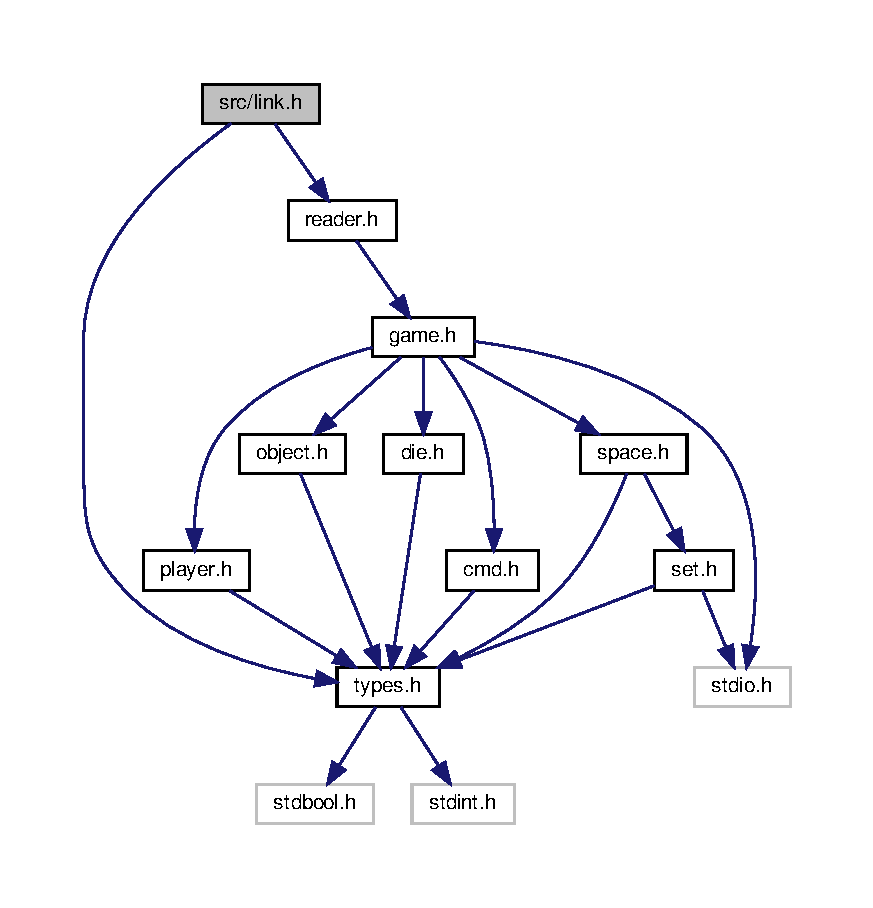
\includegraphics[width=350pt]{link_8h__incl}
\end{center}
\end{figure}
This graph shows which files directly or indirectly include this file\+:
\nopagebreak
\begin{figure}[H]
\begin{center}
\leavevmode
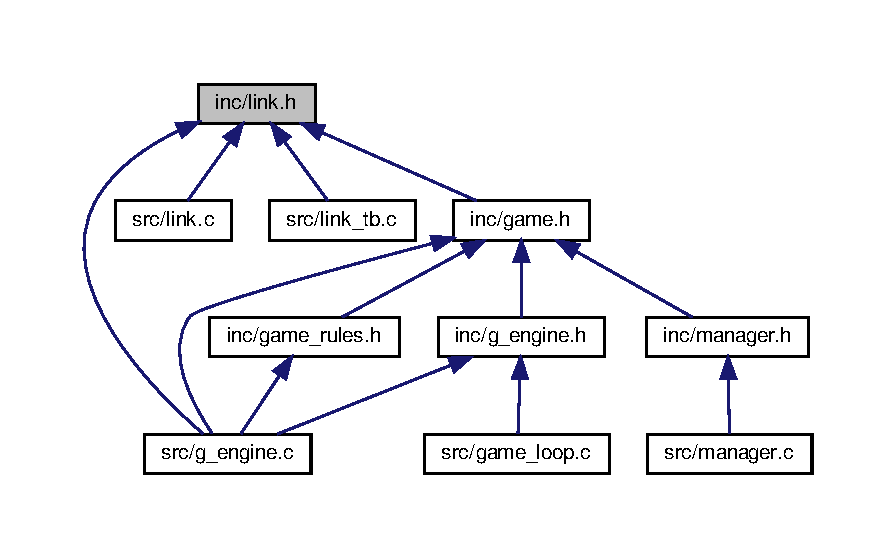
\includegraphics[width=350pt]{link_8h__dep__incl}
\end{center}
\end{figure}
\subsection*{Macros}
\begin{DoxyCompactItemize}
\item 
\mbox{\Hypertarget{link_8h_a660ed1ec8604982002a0d6eced0e0367}\label{link_8h_a660ed1ec8604982002a0d6eced0e0367}} 
\#define {\bfseries M\+A\+X\+\_\+\+L\+I\+N\+KS}~100
\item 
\mbox{\Hypertarget{link_8h_ab4477e941817afbf1649fdf3dfb62d70}\label{link_8h_ab4477e941817afbf1649fdf3dfb62d70}} 
\#define \hyperlink{link_8h_ab4477e941817afbf1649fdf3dfb62d70}{M\+A\+X\+\_\+\+L\+I\+N\+K\+\_\+\+N\+A\+ME}~100
\begin{DoxyCompactList}\small\item\em Maximum length of the link name. \end{DoxyCompactList}\end{DoxyCompactItemize}
\subsection*{Typedefs}
\begin{DoxyCompactItemize}
\item 
\mbox{\Hypertarget{link_8h_ae3b299941e67be6971bfd64a25505eff}\label{link_8h_ae3b299941e67be6971bfd64a25505eff}} 
typedef struct \hyperlink{struct__Link}{\+\_\+\+Link} {\bfseries Link}
\end{DoxyCompactItemize}
\subsection*{Enumerations}
\begin{DoxyCompactItemize}
\item 
\mbox{\Hypertarget{link_8h_ab0033b911037fd995258d117e65461e0}\label{link_8h_ab0033b911037fd995258d117e65461e0}} 
enum \hyperlink{link_8h_ab0033b911037fd995258d117e65461e0}{Link\+State} \{ {\bfseries L\+I\+N\+K\+\_\+\+O\+P\+E\+N\+ED}, 
{\bfseries L\+I\+N\+K\+\_\+\+C\+L\+O\+S\+ED}
 \}\begin{DoxyCompactList}\small\item\em The enum of the state. \end{DoxyCompactList}
\end{DoxyCompactItemize}
\subsection*{Functions}
\begin{DoxyCompactItemize}
\item 
\hyperlink{struct__Link}{Link} $\ast$ \hyperlink{link_8h_a8090d7f529cfd6a2fc5df3dd379fe514}{link\+\_\+create} (\hyperlink{types_8h_a845e604fb28f7e3d97549da3448149d3}{Id} id)
\begin{DoxyCompactList}\small\item\em initializes a new link \end{DoxyCompactList}\item 
\hyperlink{types_8h_a32c27cc471df37f4fc818d65de0a56c4}{S\+T\+A\+T\+US} \hyperlink{link_8h_a85c4dd77887bf31f651ea1162144d712}{link\+\_\+destroy} (\hyperlink{struct__Link}{Link} $\ast$link)
\begin{DoxyCompactList}\small\item\em destroys a link \end{DoxyCompactList}\item 
\hyperlink{types_8h_a845e604fb28f7e3d97549da3448149d3}{Id} \hyperlink{link_8h_a2bbd320f995a72b2ea7ea639b1c81892}{link\+\_\+get\+\_\+id} (\hyperlink{struct__Link}{Link} $\ast$link)
\begin{DoxyCompactList}\small\item\em Gets the id of a link. \end{DoxyCompactList}\item 
\hyperlink{types_8h_a845e604fb28f7e3d97549da3448149d3}{Id} \hyperlink{link_8h_a6e03d80f1a54c61a366a4a81aaca8106}{link\+\_\+get\+\_\+from} (\hyperlink{struct__Link}{Link} $\ast$link)
\begin{DoxyCompactList}\small\item\em Gets the destination id of a link. \end{DoxyCompactList}\item 
\hyperlink{types_8h_a845e604fb28f7e3d97549da3448149d3}{Id} \hyperlink{link_8h_a74cf03260545d4b8d19228aab08bdffd}{link\+\_\+get\+\_\+to} (\hyperlink{struct__Link}{Link} $\ast$link)
\begin{DoxyCompactList}\small\item\em gets the id\+To of a link \end{DoxyCompactList}\item 
const char $\ast$ \hyperlink{link_8h_aaab4c9c7d5492873cafd9e11dc0f8059}{link\+\_\+get\+\_\+name} (\hyperlink{struct__Link}{Link} $\ast$link)
\begin{DoxyCompactList}\small\item\em gets the name of a link \end{DoxyCompactList}\item 
\hyperlink{link_8h_ab0033b911037fd995258d117e65461e0}{Link\+State} \hyperlink{link_8h_acbc8c044a54ceb16e24d828370d98244}{link\+\_\+get\+\_\+state} (\hyperlink{struct__Link}{Link} $\ast$link)
\begin{DoxyCompactList}\small\item\em gets the state of a link O\+P\+EN or C\+L\+O\+SE \end{DoxyCompactList}\item 
\hyperlink{types_8h_a32c27cc471df37f4fc818d65de0a56c4}{S\+T\+A\+T\+US} \hyperlink{link_8h_a7e39694824973f396f87d8c01e9b824a}{link\+\_\+set\+\_\+state} (\hyperlink{struct__Link}{Link} $\ast$link, \hyperlink{link_8h_ab0033b911037fd995258d117e65461e0}{Link\+State} state)
\begin{DoxyCompactList}\small\item\em Sets the state of a given link. \end{DoxyCompactList}\item 
\hyperlink{types_8h_a32c27cc471df37f4fc818d65de0a56c4}{S\+T\+A\+T\+US} \hyperlink{link_8h_a3fd49fb1a3f19be4fc800ff07820cafb}{link\+\_\+set\+\_\+id} (\hyperlink{struct__Link}{Link} $\ast$link, \hyperlink{types_8h_a845e604fb28f7e3d97549da3448149d3}{Id} id)
\begin{DoxyCompactList}\small\item\em it set the id of a link on the structure \end{DoxyCompactList}\item 
\hyperlink{types_8h_a32c27cc471df37f4fc818d65de0a56c4}{S\+T\+A\+T\+US} \hyperlink{link_8h_a42c184164d057bfd337c09666315f704}{link\+\_\+set\+\_\+from} (\hyperlink{struct__Link}{Link} $\ast$link, \hyperlink{types_8h_a845e604fb28f7e3d97549da3448149d3}{Id} id\+From)
\begin{DoxyCompactList}\small\item\em it set the id\+From of a link on the structure \end{DoxyCompactList}\item 
\hyperlink{types_8h_a32c27cc471df37f4fc818d65de0a56c4}{S\+T\+A\+T\+US} \hyperlink{link_8h_ae07c2cb2a14cb510dd496433fa648431}{link\+\_\+set\+\_\+to} (\hyperlink{struct__Link}{Link} $\ast$link, \hyperlink{types_8h_a845e604fb28f7e3d97549da3448149d3}{Id} id\+To)
\begin{DoxyCompactList}\small\item\em it set the id\+To of a link on the structure \end{DoxyCompactList}\item 
\hyperlink{types_8h_a32c27cc471df37f4fc818d65de0a56c4}{S\+T\+A\+T\+US} \hyperlink{link_8h_a8cf278a0dc6226ed88166f5278d86ca7}{link\+\_\+set\+\_\+name} (\hyperlink{struct__Link}{Link} $\ast$link, const char $\ast$name)
\begin{DoxyCompactList}\small\item\em it set the id of a link on the structure \end{DoxyCompactList}\item 
\hyperlink{types_8h_a32c27cc471df37f4fc818d65de0a56c4}{S\+T\+A\+T\+US} \hyperlink{link_8h_ae42d5937c06a6efccd72041121658b09}{link\+\_\+print} (F\+I\+LE $\ast$stream, \hyperlink{struct__Link}{Link} $\ast$link)
\begin{DoxyCompactList}\small\item\em prints a link. \end{DoxyCompactList}\end{DoxyCompactItemize}


\subsection{Detailed Description}
link functions 

\begin{DoxyVersion}{Version}
0.\+0.\+3 
\end{DoxyVersion}
\begin{DoxyDate}{Date}
19/03/2019 
\end{DoxyDate}
\begin{DoxyAuthor}{Author}
Gonzalo Serrano 
\end{DoxyAuthor}
\begin{DoxyCopyright}{Copyright}
G\+NU Public License 
\end{DoxyCopyright}


\subsection{Function Documentation}
\mbox{\Hypertarget{link_8h_a8090d7f529cfd6a2fc5df3dd379fe514}\label{link_8h_a8090d7f529cfd6a2fc5df3dd379fe514}} 
\index{link.\+h@{link.\+h}!link\+\_\+create@{link\+\_\+create}}
\index{link\+\_\+create@{link\+\_\+create}!link.\+h@{link.\+h}}
\subsubsection{\texorpdfstring{link\+\_\+create()}{link\_create()}}
{\footnotesize\ttfamily \hyperlink{struct__Link}{Link}$\ast$ link\+\_\+create (\begin{DoxyParamCaption}\item[{\hyperlink{types_8h_a845e604fb28f7e3d97549da3448149d3}{Id}}]{id }\end{DoxyParamCaption})}



initializes a new link 

\begin{DoxyDate}{Date}
19/03/2019 
\end{DoxyDate}
\begin{DoxyAuthor}{Author}
\+: Gonzalo Serrano
\end{DoxyAuthor}

\begin{DoxyParams}{Parameters}
{\em \{\+Id\}} & id -\/ Link identification \\
\hline
\end{DoxyParams}

\begin{DoxyRetVals}{Return values}
{\em \{\+Link$\ast$\}} & -\/ returns a pointer to the new link \\
\hline
\end{DoxyRetVals}
\mbox{\Hypertarget{link_8h_a85c4dd77887bf31f651ea1162144d712}\label{link_8h_a85c4dd77887bf31f651ea1162144d712}} 
\index{link.\+h@{link.\+h}!link\+\_\+destroy@{link\+\_\+destroy}}
\index{link\+\_\+destroy@{link\+\_\+destroy}!link.\+h@{link.\+h}}
\subsubsection{\texorpdfstring{link\+\_\+destroy()}{link\_destroy()}}
{\footnotesize\ttfamily \hyperlink{types_8h_a32c27cc471df37f4fc818d65de0a56c4}{S\+T\+A\+T\+US} link\+\_\+destroy (\begin{DoxyParamCaption}\item[{\hyperlink{struct__Link}{Link} $\ast$}]{link }\end{DoxyParamCaption})}



destroys a link 

\begin{DoxyDate}{Date}
19/03/2019 
\end{DoxyDate}
\begin{DoxyAuthor}{Author}
Gonzalo Serrano
\end{DoxyAuthor}

\begin{DoxyParams}{Parameters}
{\em \{\+Link$\ast$\}} & link -\/ Link pointer \\
\hline
\end{DoxyParams}

\begin{DoxyRetVals}{Return values}
{\em \{void\}} & -\/ Do not returns nothing \\
\hline
\end{DoxyRetVals}
\mbox{\Hypertarget{link_8h_a2bbd320f995a72b2ea7ea639b1c81892}\label{link_8h_a2bbd320f995a72b2ea7ea639b1c81892}} 
\index{link.\+h@{link.\+h}!link\+\_\+get\+\_\+id@{link\+\_\+get\+\_\+id}}
\index{link\+\_\+get\+\_\+id@{link\+\_\+get\+\_\+id}!link.\+h@{link.\+h}}
\subsubsection{\texorpdfstring{link\+\_\+get\+\_\+id()}{link\_get\_id()}}
{\footnotesize\ttfamily \hyperlink{types_8h_a845e604fb28f7e3d97549da3448149d3}{Id} link\+\_\+get\+\_\+id (\begin{DoxyParamCaption}\item[{\hyperlink{struct__Link}{Link} $\ast$}]{link }\end{DoxyParamCaption})}



Gets the id of a link. 

\begin{DoxyDate}{Date}
19/03/2019 
\end{DoxyDate}
\begin{DoxyAuthor}{Author}
Gonzalo Serrano
\end{DoxyAuthor}

\begin{DoxyParams}{Parameters}
{\em \{\+Link$\ast$\}} & link -\/ Link pointer \\
\hline
\end{DoxyParams}

\begin{DoxyRetVals}{Return values}
{\em \{\+Id\}} & -\/ Returns the id of a link \\
\hline
\end{DoxyRetVals}
\mbox{\Hypertarget{link_8h_a6e03d80f1a54c61a366a4a81aaca8106}\label{link_8h_a6e03d80f1a54c61a366a4a81aaca8106}} 
\index{link.\+h@{link.\+h}!link\+\_\+get\+\_\+from@{link\+\_\+get\+\_\+from}}
\index{link\+\_\+get\+\_\+from@{link\+\_\+get\+\_\+from}!link.\+h@{link.\+h}}
\subsubsection{\texorpdfstring{link\+\_\+get\+\_\+from()}{link\_get\_from()}}
{\footnotesize\ttfamily \hyperlink{types_8h_a845e604fb28f7e3d97549da3448149d3}{Id} link\+\_\+get\+\_\+from (\begin{DoxyParamCaption}\item[{\hyperlink{struct__Link}{Link} $\ast$}]{link }\end{DoxyParamCaption})}



Gets the destination id of a link. 

\begin{DoxyDate}{Date}
19/03/2019 
\end{DoxyDate}
\begin{DoxyAuthor}{Author}
Gonzalo Serrano
\end{DoxyAuthor}

\begin{DoxyParams}{Parameters}
{\em \{\+Link$\ast$\}} & link -\/ Link pointer \\
\hline
\end{DoxyParams}

\begin{DoxyRetVals}{Return values}
{\em \{\+Id\}} & -\/ Returns the id\+From of a link \\
\hline
\end{DoxyRetVals}
\mbox{\Hypertarget{link_8h_a74cf03260545d4b8d19228aab08bdffd}\label{link_8h_a74cf03260545d4b8d19228aab08bdffd}} 
\index{link.\+h@{link.\+h}!link\+\_\+get\+\_\+to@{link\+\_\+get\+\_\+to}}
\index{link\+\_\+get\+\_\+to@{link\+\_\+get\+\_\+to}!link.\+h@{link.\+h}}
\subsubsection{\texorpdfstring{link\+\_\+get\+\_\+to()}{link\_get\_to()}}
{\footnotesize\ttfamily \hyperlink{types_8h_a845e604fb28f7e3d97549da3448149d3}{Id} link\+\_\+get\+\_\+to (\begin{DoxyParamCaption}\item[{\hyperlink{struct__Link}{Link} $\ast$}]{link }\end{DoxyParamCaption})}



gets the id\+To of a link 

\begin{DoxyDate}{Date}
19/03/2019 
\end{DoxyDate}
\begin{DoxyAuthor}{Author}
Gonzalo Serrano
\end{DoxyAuthor}

\begin{DoxyParams}{Parameters}
{\em \{\+Link$\ast$\}} & link -\/ Link pointer \\
\hline
\end{DoxyParams}

\begin{DoxyRetVals}{Return values}
{\em \{\+Id\}} & -\/ Returns the id\+To of a link \\
\hline
\end{DoxyRetVals}
\mbox{\Hypertarget{link_8h_aaab4c9c7d5492873cafd9e11dc0f8059}\label{link_8h_aaab4c9c7d5492873cafd9e11dc0f8059}} 
\index{link.\+h@{link.\+h}!link\+\_\+get\+\_\+name@{link\+\_\+get\+\_\+name}}
\index{link\+\_\+get\+\_\+name@{link\+\_\+get\+\_\+name}!link.\+h@{link.\+h}}
\subsubsection{\texorpdfstring{link\+\_\+get\+\_\+name()}{link\_get\_name()}}
{\footnotesize\ttfamily const char$\ast$ link\+\_\+get\+\_\+name (\begin{DoxyParamCaption}\item[{\hyperlink{struct__Link}{Link} $\ast$}]{link }\end{DoxyParamCaption})}



gets the name of a link 

\begin{DoxyDate}{Date}
19/03/2019 
\end{DoxyDate}
\begin{DoxyAuthor}{Author}
Gonzalo Serrano
\end{DoxyAuthor}

\begin{DoxyParams}{Parameters}
{\em \{\+Link$\ast$\}} & link -\/ Link pointer \\
\hline
\end{DoxyParams}

\begin{DoxyRetVals}{Return values}
{\em \{\+Id\}} & -\/ Returns the name of a link \\
\hline
\end{DoxyRetVals}
\mbox{\Hypertarget{link_8h_acbc8c044a54ceb16e24d828370d98244}\label{link_8h_acbc8c044a54ceb16e24d828370d98244}} 
\index{link.\+h@{link.\+h}!link\+\_\+get\+\_\+state@{link\+\_\+get\+\_\+state}}
\index{link\+\_\+get\+\_\+state@{link\+\_\+get\+\_\+state}!link.\+h@{link.\+h}}
\subsubsection{\texorpdfstring{link\+\_\+get\+\_\+state()}{link\_get\_state()}}
{\footnotesize\ttfamily \hyperlink{link_8h_ab0033b911037fd995258d117e65461e0}{Link\+State} link\+\_\+get\+\_\+state (\begin{DoxyParamCaption}\item[{\hyperlink{struct__Link}{Link} $\ast$}]{link }\end{DoxyParamCaption})}



gets the state of a link O\+P\+EN or C\+L\+O\+SE 

\begin{DoxyDate}{Date}
19/03/2019 
\end{DoxyDate}
\begin{DoxyAuthor}{Author}
Gonzalo Serrano
\end{DoxyAuthor}

\begin{DoxyParams}{Parameters}
{\em \{\+Link$\ast$\}} & link -\/ Link pointer \\
\hline
\end{DoxyParams}

\begin{DoxyRetVals}{Return values}
{\em \{\+Link\+State\}} & -\/ Returns the state of a link \\
\hline
\end{DoxyRetVals}
\mbox{\Hypertarget{link_8h_a7e39694824973f396f87d8c01e9b824a}\label{link_8h_a7e39694824973f396f87d8c01e9b824a}} 
\index{link.\+h@{link.\+h}!link\+\_\+set\+\_\+state@{link\+\_\+set\+\_\+state}}
\index{link\+\_\+set\+\_\+state@{link\+\_\+set\+\_\+state}!link.\+h@{link.\+h}}
\subsubsection{\texorpdfstring{link\+\_\+set\+\_\+state()}{link\_set\_state()}}
{\footnotesize\ttfamily \hyperlink{types_8h_a32c27cc471df37f4fc818d65de0a56c4}{S\+T\+A\+T\+US} link\+\_\+set\+\_\+state (\begin{DoxyParamCaption}\item[{\hyperlink{struct__Link}{Link} $\ast$}]{link,  }\item[{\hyperlink{link_8h_ab0033b911037fd995258d117e65461e0}{Link\+State}}]{state }\end{DoxyParamCaption})}



Sets the state of a given link. 

\begin{DoxyDate}{Date}
19/03/2019 
\end{DoxyDate}
\begin{DoxyAuthor}{Author}
Gonzalo Serrano
\end{DoxyAuthor}

\begin{DoxyParams}{Parameters}
{\em \{\+Link$\ast$\}} & link -\/ Link pointer \\
\hline
{\em \{\+Link\+State\}} & id -\/ New state of the link \\
\hline
\end{DoxyParams}
\begin{DoxyReturn}{Returns}
\{S\+T\+A\+T\+US\} -\/ Returns an status 
\end{DoxyReturn}
\mbox{\Hypertarget{link_8h_a3fd49fb1a3f19be4fc800ff07820cafb}\label{link_8h_a3fd49fb1a3f19be4fc800ff07820cafb}} 
\index{link.\+h@{link.\+h}!link\+\_\+set\+\_\+id@{link\+\_\+set\+\_\+id}}
\index{link\+\_\+set\+\_\+id@{link\+\_\+set\+\_\+id}!link.\+h@{link.\+h}}
\subsubsection{\texorpdfstring{link\+\_\+set\+\_\+id()}{link\_set\_id()}}
{\footnotesize\ttfamily \hyperlink{types_8h_a32c27cc471df37f4fc818d65de0a56c4}{S\+T\+A\+T\+US} link\+\_\+set\+\_\+id (\begin{DoxyParamCaption}\item[{\hyperlink{struct__Link}{Link} $\ast$}]{link,  }\item[{\hyperlink{types_8h_a845e604fb28f7e3d97549da3448149d3}{Id}}]{id }\end{DoxyParamCaption})}



it set the id of a link on the structure 

\begin{DoxyDate}{Date}
19/03/2019 
\end{DoxyDate}
\begin{DoxyAuthor}{Author}
Gonzalo Serrano
\end{DoxyAuthor}

\begin{DoxyParams}{Parameters}
{\em \{\+Link$\ast$\}} & link -\/ Link pointer \\
\hline
{\em \{\+Id\}} & id -\/ id of a link \\
\hline
\end{DoxyParams}
\begin{DoxyReturn}{Returns}
\{S\+T\+A\+T\+US\} -\/ Returns an status 
\end{DoxyReturn}
\mbox{\Hypertarget{link_8h_a42c184164d057bfd337c09666315f704}\label{link_8h_a42c184164d057bfd337c09666315f704}} 
\index{link.\+h@{link.\+h}!link\+\_\+set\+\_\+from@{link\+\_\+set\+\_\+from}}
\index{link\+\_\+set\+\_\+from@{link\+\_\+set\+\_\+from}!link.\+h@{link.\+h}}
\subsubsection{\texorpdfstring{link\+\_\+set\+\_\+from()}{link\_set\_from()}}
{\footnotesize\ttfamily \hyperlink{types_8h_a32c27cc471df37f4fc818d65de0a56c4}{S\+T\+A\+T\+US} link\+\_\+set\+\_\+from (\begin{DoxyParamCaption}\item[{\hyperlink{struct__Link}{Link} $\ast$}]{link,  }\item[{\hyperlink{types_8h_a845e604fb28f7e3d97549da3448149d3}{Id}}]{id\+From }\end{DoxyParamCaption})}



it set the id\+From of a link on the structure 

\begin{DoxyDate}{Date}
19/03/2019 
\end{DoxyDate}
\begin{DoxyAuthor}{Author}
Gonzalo Serrano
\end{DoxyAuthor}

\begin{DoxyParams}{Parameters}
{\em \{\+Link$\ast$\}} & link -\/ Link pointer \\
\hline
{\em \{\+Id\}} & id\+From -\/ id\+From of a link \\
\hline
\end{DoxyParams}
\begin{DoxyReturn}{Returns}
\{S\+T\+A\+T\+US\} -\/ Returns an status 
\end{DoxyReturn}
\mbox{\Hypertarget{link_8h_ae07c2cb2a14cb510dd496433fa648431}\label{link_8h_ae07c2cb2a14cb510dd496433fa648431}} 
\index{link.\+h@{link.\+h}!link\+\_\+set\+\_\+to@{link\+\_\+set\+\_\+to}}
\index{link\+\_\+set\+\_\+to@{link\+\_\+set\+\_\+to}!link.\+h@{link.\+h}}
\subsubsection{\texorpdfstring{link\+\_\+set\+\_\+to()}{link\_set\_to()}}
{\footnotesize\ttfamily \hyperlink{types_8h_a32c27cc471df37f4fc818d65de0a56c4}{S\+T\+A\+T\+US} link\+\_\+set\+\_\+to (\begin{DoxyParamCaption}\item[{\hyperlink{struct__Link}{Link} $\ast$}]{link,  }\item[{\hyperlink{types_8h_a845e604fb28f7e3d97549da3448149d3}{Id}}]{id\+To }\end{DoxyParamCaption})}



it set the id\+To of a link on the structure 

\begin{DoxyDate}{Date}
19/03/2019 
\end{DoxyDate}
\begin{DoxyAuthor}{Author}
Gonzalo Serrano
\end{DoxyAuthor}

\begin{DoxyParams}{Parameters}
{\em \{\+Link$\ast$\}} & link -\/ Link pointer \\
\hline
{\em \{\+Id\}} & id\+To -\/ id\+To of a link \\
\hline
\end{DoxyParams}
\begin{DoxyReturn}{Returns}
\{S\+T\+A\+T\+US\} -\/ Returns an status 
\end{DoxyReturn}
\mbox{\Hypertarget{link_8h_a8cf278a0dc6226ed88166f5278d86ca7}\label{link_8h_a8cf278a0dc6226ed88166f5278d86ca7}} 
\index{link.\+h@{link.\+h}!link\+\_\+set\+\_\+name@{link\+\_\+set\+\_\+name}}
\index{link\+\_\+set\+\_\+name@{link\+\_\+set\+\_\+name}!link.\+h@{link.\+h}}
\subsubsection{\texorpdfstring{link\+\_\+set\+\_\+name()}{link\_set\_name()}}
{\footnotesize\ttfamily \hyperlink{types_8h_a32c27cc471df37f4fc818d65de0a56c4}{S\+T\+A\+T\+US} link\+\_\+set\+\_\+name (\begin{DoxyParamCaption}\item[{\hyperlink{struct__Link}{Link} $\ast$}]{link,  }\item[{const char $\ast$}]{name }\end{DoxyParamCaption})}



it set the id of a link on the structure 

\begin{DoxyDate}{Date}
19/03/2019 
\end{DoxyDate}
\begin{DoxyAuthor}{Author}
Gonzalo Serrano
\end{DoxyAuthor}

\begin{DoxyParams}{Parameters}
{\em \{\+Link$\ast$\}} & link -\/ Link pointer \\
\hline
{\em \{name\}} & -\/ Link name \\
\hline
\end{DoxyParams}
\begin{DoxyReturn}{Returns}
\{S\+T\+A\+T\+US\} -\/ Returns an status 
\end{DoxyReturn}
\mbox{\Hypertarget{link_8h_ae42d5937c06a6efccd72041121658b09}\label{link_8h_ae42d5937c06a6efccd72041121658b09}} 
\index{link.\+h@{link.\+h}!link\+\_\+print@{link\+\_\+print}}
\index{link\+\_\+print@{link\+\_\+print}!link.\+h@{link.\+h}}
\subsubsection{\texorpdfstring{link\+\_\+print()}{link\_print()}}
{\footnotesize\ttfamily \hyperlink{types_8h_a32c27cc471df37f4fc818d65de0a56c4}{S\+T\+A\+T\+US} link\+\_\+print (\begin{DoxyParamCaption}\item[{F\+I\+LE $\ast$}]{stream,  }\item[{\hyperlink{struct__Link}{Link} $\ast$}]{link }\end{DoxyParamCaption})}



prints a link. 

\begin{DoxyDate}{Date}
19/03/2019 
\end{DoxyDate}
\begin{DoxyAuthor}{Author}
Gonzalo Serrano
\end{DoxyAuthor}

\begin{DoxyParams}{Parameters}
{\em \{\+F\+I\+L\+E$\ast$\}} & stream -\/ Streaming output \\
\hline
{\em \{\+Link$\ast$\}} & link -\/ Link pointer \\
\hline
\end{DoxyParams}
\begin{DoxyReturn}{Returns}
\{S\+T\+A\+T\+US\} -\/ Returns an status 
\end{DoxyReturn}

\hypertarget{log_8h}{}\section{inc/log.h File Reference}
\label{log_8h}\index{inc/log.\+h@{inc/log.\+h}}


Logger.  


{\ttfamily \#include $<$stdbool.\+h$>$}\newline
Include dependency graph for log.\+h\+:\nopagebreak
\begin{figure}[H]
\begin{center}
\leavevmode
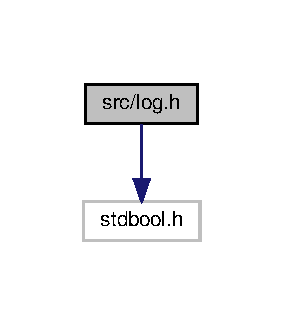
\includegraphics[width=136pt]{log_8h__incl}
\end{center}
\end{figure}
This graph shows which files directly or indirectly include this file\+:
\nopagebreak
\begin{figure}[H]
\begin{center}
\leavevmode
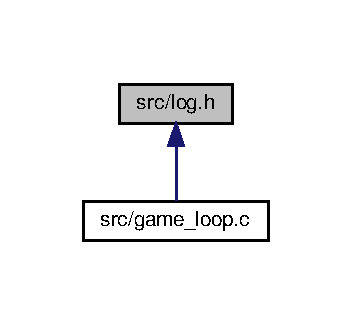
\includegraphics[width=169pt]{log_8h__dep__incl}
\end{center}
\end{figure}
\subsection*{Functions}
\begin{DoxyCompactItemize}
\item 
void \hyperlink{log_8h_a0c91588938d1cce9d3e9cb940054cd0c}{log\+\_\+begin} (const char $\ast$log\+\_\+n)
\begin{DoxyCompactList}\small\item\em initializes the file \end{DoxyCompactList}\item 
void \hyperlink{log_8h_a364f0afe48f0446c287eb861e30672e5}{log\+\_\+w} (const char $\ast$frm,...)
\begin{DoxyCompactList}\small\item\em writes in the file \end{DoxyCompactList}\item 
void \hyperlink{log_8h_a73e93b618b1802ac18d6e6d81b246378}{log\+\_\+end} ()
\begin{DoxyCompactList}\small\item\em it closes the file opened before \end{DoxyCompactList}\item 
bool \hyperlink{log_8h_a91c077066e868dc9488657aaf84d911d}{log\+\_\+is\+Open} ()
\begin{DoxyCompactList}\small\item\em it checks if the log file is open \end{DoxyCompactList}\end{DoxyCompactItemize}


\subsection{Detailed Description}
Logger. 

\begin{DoxyVersion}{Version}
0.\+3.\+3 
\end{DoxyVersion}
\begin{DoxyDate}{Date}
16/02/2019 
\end{DoxyDate}
\begin{DoxyAuthor}{Author}
Javier Romera 
\end{DoxyAuthor}
\begin{DoxyCopyright}{Copyright}
G\+NU Public License 
\end{DoxyCopyright}


\subsection{Function Documentation}
\mbox{\Hypertarget{log_8h_a0c91588938d1cce9d3e9cb940054cd0c}\label{log_8h_a0c91588938d1cce9d3e9cb940054cd0c}} 
\index{log.\+h@{log.\+h}!log\+\_\+begin@{log\+\_\+begin}}
\index{log\+\_\+begin@{log\+\_\+begin}!log.\+h@{log.\+h}}
\subsubsection{\texorpdfstring{log\+\_\+begin()}{log\_begin()}}
{\footnotesize\ttfamily void log\+\_\+begin (\begin{DoxyParamCaption}\item[{const char $\ast$}]{log\+\_\+n }\end{DoxyParamCaption})}



initializes the file 

\begin{DoxyDate}{Date}
16/02/2019 
\end{DoxyDate}
\begin{DoxyAuthor}{Author}
Javier Romera
\end{DoxyAuthor}

\begin{DoxyParams}{Parameters}
{\em \{const} & char$\ast$\} log\+\_\+n -\/ Log name \\
\hline
\end{DoxyParams}
\mbox{\Hypertarget{log_8h_a364f0afe48f0446c287eb861e30672e5}\label{log_8h_a364f0afe48f0446c287eb861e30672e5}} 
\index{log.\+h@{log.\+h}!log\+\_\+w@{log\+\_\+w}}
\index{log\+\_\+w@{log\+\_\+w}!log.\+h@{log.\+h}}
\subsubsection{\texorpdfstring{log\+\_\+w()}{log\_w()}}
{\footnotesize\ttfamily void log\+\_\+w (\begin{DoxyParamCaption}\item[{const char $\ast$}]{frm,  }\item[{}]{... }\end{DoxyParamCaption})}



writes in the file 

\begin{DoxyDate}{Date}
16/02/2019 
\end{DoxyDate}
\begin{DoxyAuthor}{Author}
Javier Romera
\end{DoxyAuthor}

\begin{DoxyParams}{Parameters}
{\em \{const} & char$\ast$\} frm -\/ String format \\
\hline
{\em \{...\}} & -\/ String format arguments \\
\hline
\end{DoxyParams}
\mbox{\Hypertarget{log_8h_a73e93b618b1802ac18d6e6d81b246378}\label{log_8h_a73e93b618b1802ac18d6e6d81b246378}} 
\index{log.\+h@{log.\+h}!log\+\_\+end@{log\+\_\+end}}
\index{log\+\_\+end@{log\+\_\+end}!log.\+h@{log.\+h}}
\subsubsection{\texorpdfstring{log\+\_\+end()}{log\_end()}}
{\footnotesize\ttfamily void log\+\_\+end (\begin{DoxyParamCaption}{ }\end{DoxyParamCaption})}



it closes the file opened before 

\begin{DoxyDate}{Date}
16/02/2019 
\end{DoxyDate}
\begin{DoxyAuthor}{Author}
Javier Romera 
\end{DoxyAuthor}

\begin{DoxyParams}{Parameters}
{\em \{char$\ast$\}} & frm -\/ String format \\
\hline
{\em \{...\}} & -\/ String format arguments \\
\hline
\end{DoxyParams}
\mbox{\Hypertarget{log_8h_a91c077066e868dc9488657aaf84d911d}\label{log_8h_a91c077066e868dc9488657aaf84d911d}} 
\index{log.\+h@{log.\+h}!log\+\_\+is\+Open@{log\+\_\+is\+Open}}
\index{log\+\_\+is\+Open@{log\+\_\+is\+Open}!log.\+h@{log.\+h}}
\subsubsection{\texorpdfstring{log\+\_\+is\+Open()}{log\_isOpen()}}
{\footnotesize\ttfamily bool log\+\_\+is\+Open (\begin{DoxyParamCaption}{ }\end{DoxyParamCaption})}



it checks if the log file is open 

\begin{DoxyDate}{Date}
16/02/2019 
\end{DoxyDate}
\begin{DoxyAuthor}{Author}
Javier Romera
\end{DoxyAuthor}

\begin{DoxyParams}{Parameters}
{\em empty} & \\
\hline
\end{DoxyParams}

\begin{DoxyRetVals}{Return values}
{\em \{bool\}} & -\/ Returns False or True \\
\hline
\end{DoxyRetVals}

\hypertarget{object_8h}{}\section{inc/object.h File Reference}
\label{object_8h}\index{inc/object.\+h@{inc/object.\+h}}


Object manager.  


{\ttfamily \#include \char`\"{}types.\+h\char`\"{}}\newline
Include dependency graph for object.\+h\+:\nopagebreak
\begin{figure}[H]
\begin{center}
\leavevmode
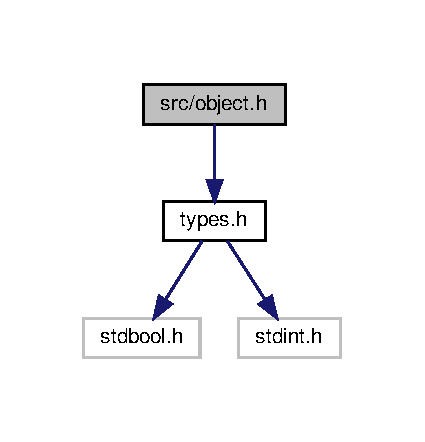
\includegraphics[width=204pt]{object_8h__incl}
\end{center}
\end{figure}
This graph shows which files directly or indirectly include this file\+:\nopagebreak
\begin{figure}[H]
\begin{center}
\leavevmode
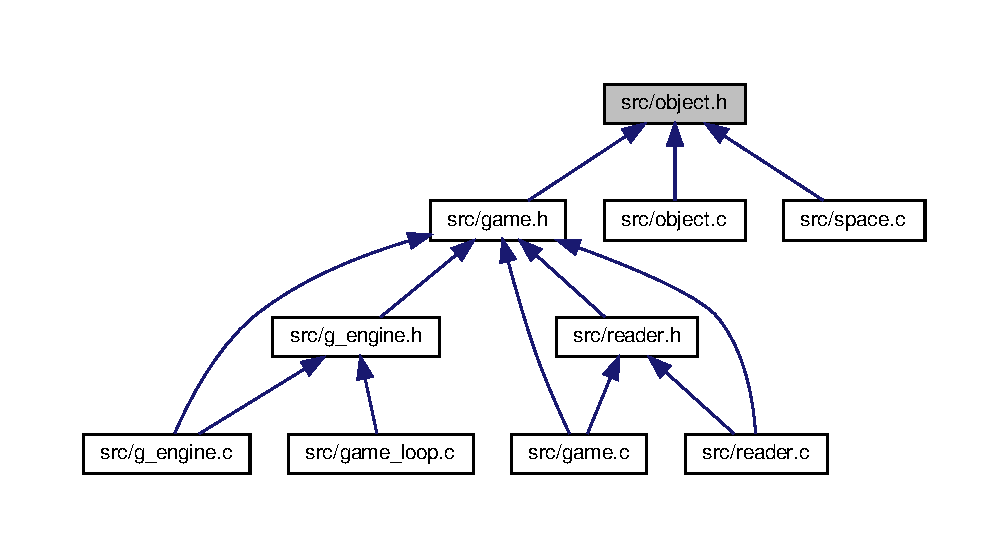
\includegraphics[width=350pt]{object_8h__dep__incl}
\end{center}
\end{figure}
\subsection*{Macros}
\begin{DoxyCompactItemize}
\item 
\mbox{\Hypertarget{object_8h_a9c396da2f3b9f0191120ff1666af6381}\label{object_8h_a9c396da2f3b9f0191120ff1666af6381}} 
\#define \hyperlink{object_8h_a9c396da2f3b9f0191120ff1666af6381}{M\+A\+X\+\_\+\+O\+B\+J\+\_\+\+D\+E\+S\+C\+RP}~100
\begin{DoxyCompactList}\small\item\em Maximum number of characters that can have a description of an object. \end{DoxyCompactList}\item 
\mbox{\Hypertarget{object_8h_a6a2f391825e94d06a3137b75abfa1bba}\label{object_8h_a6a2f391825e94d06a3137b75abfa1bba}} 
\#define \hyperlink{object_8h_a6a2f391825e94d06a3137b75abfa1bba}{M\+A\+X\+\_\+\+O\+B\+J\+\_\+\+N\+A\+ME}~50
\begin{DoxyCompactList}\small\item\em Maximum number of characters that can have a name of an object. \end{DoxyCompactList}\item 
\mbox{\Hypertarget{object_8h_acdc7844fbd4d45737d4aa56834d37829}\label{object_8h_acdc7844fbd4d45737d4aa56834d37829}} 
\#define \hyperlink{object_8h_acdc7844fbd4d45737d4aa56834d37829}{M\+A\+X\+\_\+\+O\+B\+J\+E\+C\+TS}~4
\begin{DoxyCompactList}\small\item\em Maximum number of objects. \end{DoxyCompactList}\end{DoxyCompactItemize}
\subsection*{Typedefs}
\begin{DoxyCompactItemize}
\item 
\mbox{\Hypertarget{object_8h_a7f8bbcda919b65ce67f92fba08e0212f}\label{object_8h_a7f8bbcda919b65ce67f92fba08e0212f}} 
typedef struct \hyperlink{struct__Object}{\+\_\+\+Object} \hyperlink{object_8h_a7f8bbcda919b65ce67f92fba08e0212f}{Object}
\begin{DoxyCompactList}\small\item\em Defines the type of object structure. \end{DoxyCompactList}\end{DoxyCompactItemize}
\subsection*{Functions}
\begin{DoxyCompactItemize}
\item 
\hyperlink{object_8h_a7f8bbcda919b65ce67f92fba08e0212f}{Object} $\ast$ \hyperlink{object_8h_a1196be6af8524bec98758a054f146c66}{obj\+\_\+create} (\hyperlink{types_8h_a845e604fb28f7e3d97549da3448149d3}{Id} id)
\begin{DoxyCompactList}\small\item\em This fuction initializes an object. \end{DoxyCompactList}\item 
void \hyperlink{object_8h_ac9aeb62f8e8555a59661cca384db6b47}{obj\+\_\+destroy} (\hyperlink{object_8h_a7f8bbcda919b65ce67f92fba08e0212f}{Object} $\ast$obj)
\begin{DoxyCompactList}\small\item\em This fuction destroys an object. \end{DoxyCompactList}\item 
\hyperlink{types_8h_a32c27cc471df37f4fc818d65de0a56c4}{S\+T\+A\+T\+US} \hyperlink{object_8h_ae3a067d875771850a14394d99d3d0d8a}{obj\+\_\+set\+\_\+name} (\hyperlink{object_8h_a7f8bbcda919b65ce67f92fba08e0212f}{Object} $\ast$obj, const char $\ast$name)
\begin{DoxyCompactList}\small\item\em This fuction sets an object name. \end{DoxyCompactList}\item 
const char $\ast$ \hyperlink{object_8h_a9592df618edfeffbb0cf0ae098e06ac7}{obj\+\_\+get\+\_\+name} (\hyperlink{object_8h_a7f8bbcda919b65ce67f92fba08e0212f}{Object} $\ast$obj)
\begin{DoxyCompactList}\small\item\em This fuction gets an object name. \end{DoxyCompactList}\item 
\hyperlink{types_8h_a32c27cc471df37f4fc818d65de0a56c4}{S\+T\+A\+T\+US} \hyperlink{object_8h_ace63935d0c25ea9b4b856530b958d126}{obj\+\_\+set\+\_\+descrp} (\hyperlink{object_8h_a7f8bbcda919b65ce67f92fba08e0212f}{Object} $\ast$obj, const char $\ast$descrp)
\begin{DoxyCompactList}\small\item\em This fuction sets the description of an object. \end{DoxyCompactList}\item 
const char $\ast$ \hyperlink{object_8h_a4f5633be628368d20545ecce98f1a94a}{obj\+\_\+get\+\_\+descrp} (\hyperlink{object_8h_a7f8bbcda919b65ce67f92fba08e0212f}{Object} $\ast$obj)
\begin{DoxyCompactList}\small\item\em This fuction gets the description of an object. \end{DoxyCompactList}\item 
\hyperlink{types_8h_a32c27cc471df37f4fc818d65de0a56c4}{S\+T\+A\+T\+US} \hyperlink{object_8h_aae31252e170615356965581cde5c2e9c}{obj\+\_\+set\+\_\+id} (\hyperlink{object_8h_a7f8bbcda919b65ce67f92fba08e0212f}{Object} $\ast$obj, const \hyperlink{types_8h_a845e604fb28f7e3d97549da3448149d3}{Id} id)
\begin{DoxyCompactList}\small\item\em This fuction sets the object id. \end{DoxyCompactList}\item 
const \hyperlink{types_8h_a845e604fb28f7e3d97549da3448149d3}{Id} \hyperlink{object_8h_a7241dbfc246b252ee486f31519794922}{obj\+\_\+get\+\_\+id} (\hyperlink{object_8h_a7f8bbcda919b65ce67f92fba08e0212f}{Object} $\ast$obj)
\begin{DoxyCompactList}\small\item\em This fuction gets the object id. \end{DoxyCompactList}\end{DoxyCompactItemize}


\subsection{Detailed Description}
Object manager. 

\begin{DoxyVersion}{Version}
0.\+9.\+1 
\end{DoxyVersion}
\begin{DoxyDate}{Date}
18/03/2019 
\end{DoxyDate}


\subsection{Function Documentation}
\mbox{\Hypertarget{object_8h_a1196be6af8524bec98758a054f146c66}\label{object_8h_a1196be6af8524bec98758a054f146c66}} 
\index{object.\+h@{object.\+h}!obj\+\_\+create@{obj\+\_\+create}}
\index{obj\+\_\+create@{obj\+\_\+create}!object.\+h@{object.\+h}}
\subsubsection{\texorpdfstring{obj\+\_\+create()}{obj\_create()}}
{\footnotesize\ttfamily \hyperlink{object_8h_a7f8bbcda919b65ce67f92fba08e0212f}{Object}$\ast$ obj\+\_\+create (\begin{DoxyParamCaption}\item[{\hyperlink{types_8h_a845e604fb28f7e3d97549da3448149d3}{Id}}]{id }\end{DoxyParamCaption})}



This fuction initializes an object. 

\begin{DoxyAuthor}{Author}
Miguel Rodríguez 
\end{DoxyAuthor}

\begin{DoxyParams}{Parameters}
{\em \{\+Id\}} & -\/ Object identification \\
\hline
\end{DoxyParams}

\begin{DoxyRetVals}{Return values}
{\em \{\+Object$\ast$\}} & -\/ Returns an object\textquotesingle{}s pointer \\
\hline
\end{DoxyRetVals}
\mbox{\Hypertarget{object_8h_ac9aeb62f8e8555a59661cca384db6b47}\label{object_8h_ac9aeb62f8e8555a59661cca384db6b47}} 
\index{object.\+h@{object.\+h}!obj\+\_\+destroy@{obj\+\_\+destroy}}
\index{obj\+\_\+destroy@{obj\+\_\+destroy}!object.\+h@{object.\+h}}
\subsubsection{\texorpdfstring{obj\+\_\+destroy()}{obj\_destroy()}}
{\footnotesize\ttfamily void obj\+\_\+destroy (\begin{DoxyParamCaption}\item[{\hyperlink{object_8h_a7f8bbcda919b65ce67f92fba08e0212f}{Object} $\ast$}]{obj }\end{DoxyParamCaption})}



This fuction destroys an object. 

\begin{DoxyAuthor}{Author}
Miguel Rodríguez 
\end{DoxyAuthor}

\begin{DoxyParams}{Parameters}
{\em \{\+Object$\ast$\}} & obj -\/ object pointer \\
\hline
\end{DoxyParams}
\mbox{\Hypertarget{object_8h_ae3a067d875771850a14394d99d3d0d8a}\label{object_8h_ae3a067d875771850a14394d99d3d0d8a}} 
\index{object.\+h@{object.\+h}!obj\+\_\+set\+\_\+name@{obj\+\_\+set\+\_\+name}}
\index{obj\+\_\+set\+\_\+name@{obj\+\_\+set\+\_\+name}!object.\+h@{object.\+h}}
\subsubsection{\texorpdfstring{obj\+\_\+set\+\_\+name()}{obj\_set\_name()}}
{\footnotesize\ttfamily \hyperlink{types_8h_a32c27cc471df37f4fc818d65de0a56c4}{S\+T\+A\+T\+US} obj\+\_\+set\+\_\+name (\begin{DoxyParamCaption}\item[{\hyperlink{object_8h_a7f8bbcda919b65ce67f92fba08e0212f}{Object} $\ast$}]{obj,  }\item[{const char $\ast$}]{name }\end{DoxyParamCaption})}



This fuction sets an object name. 

\begin{DoxyAuthor}{Author}
Miguel Rodríguez 
\end{DoxyAuthor}

\begin{DoxyParams}{Parameters}
{\em \{\+Object$\ast$\}} & obj -\/ object pointer \\
\hline
{\em \{char$\ast$\}} & name -\/ object\textquotesingle{}s name \\
\hline
\end{DoxyParams}
\mbox{\Hypertarget{object_8h_a9592df618edfeffbb0cf0ae098e06ac7}\label{object_8h_a9592df618edfeffbb0cf0ae098e06ac7}} 
\index{object.\+h@{object.\+h}!obj\+\_\+get\+\_\+name@{obj\+\_\+get\+\_\+name}}
\index{obj\+\_\+get\+\_\+name@{obj\+\_\+get\+\_\+name}!object.\+h@{object.\+h}}
\subsubsection{\texorpdfstring{obj\+\_\+get\+\_\+name()}{obj\_get\_name()}}
{\footnotesize\ttfamily const char$\ast$ obj\+\_\+get\+\_\+name (\begin{DoxyParamCaption}\item[{\hyperlink{object_8h_a7f8bbcda919b65ce67f92fba08e0212f}{Object} $\ast$}]{obj }\end{DoxyParamCaption})}



This fuction gets an object name. 

\begin{DoxyAuthor}{Author}
Miguel Rodríguez 
\end{DoxyAuthor}

\begin{DoxyParams}{Parameters}
{\em \{\+Object$\ast$\}} & obj -\/ object\textquotesingle{}s pointer \\
\hline
\end{DoxyParams}

\begin{DoxyRetVals}{Return values}
{\em \{char$\ast$\}} & -\/ Returns a pointer to the object\textquotesingle{}s name \\
\hline
\end{DoxyRetVals}
\mbox{\Hypertarget{object_8h_ace63935d0c25ea9b4b856530b958d126}\label{object_8h_ace63935d0c25ea9b4b856530b958d126}} 
\index{object.\+h@{object.\+h}!obj\+\_\+set\+\_\+descrp@{obj\+\_\+set\+\_\+descrp}}
\index{obj\+\_\+set\+\_\+descrp@{obj\+\_\+set\+\_\+descrp}!object.\+h@{object.\+h}}
\subsubsection{\texorpdfstring{obj\+\_\+set\+\_\+descrp()}{obj\_set\_descrp()}}
{\footnotesize\ttfamily \hyperlink{types_8h_a32c27cc471df37f4fc818d65de0a56c4}{S\+T\+A\+T\+US} obj\+\_\+set\+\_\+descrp (\begin{DoxyParamCaption}\item[{\hyperlink{object_8h_a7f8bbcda919b65ce67f92fba08e0212f}{Object} $\ast$}]{obj,  }\item[{const char $\ast$}]{descrp }\end{DoxyParamCaption})}



This fuction sets the description of an object. 

\begin{DoxyAuthor}{Author}
Miguel Rodríguez 
\end{DoxyAuthor}

\begin{DoxyParams}{Parameters}
{\em \{\+Object$\ast$\}} & obj -\/ object\textquotesingle{}s pointer \\
\hline
{\em \{char$\ast$\}} & name -\/ object\textquotesingle{}s description \\
\hline
\end{DoxyParams}
\mbox{\Hypertarget{object_8h_a4f5633be628368d20545ecce98f1a94a}\label{object_8h_a4f5633be628368d20545ecce98f1a94a}} 
\index{object.\+h@{object.\+h}!obj\+\_\+get\+\_\+descrp@{obj\+\_\+get\+\_\+descrp}}
\index{obj\+\_\+get\+\_\+descrp@{obj\+\_\+get\+\_\+descrp}!object.\+h@{object.\+h}}
\subsubsection{\texorpdfstring{obj\+\_\+get\+\_\+descrp()}{obj\_get\_descrp()}}
{\footnotesize\ttfamily const char$\ast$ obj\+\_\+get\+\_\+descrp (\begin{DoxyParamCaption}\item[{\hyperlink{object_8h_a7f8bbcda919b65ce67f92fba08e0212f}{Object} $\ast$}]{obj }\end{DoxyParamCaption})}



This fuction gets the description of an object. 

\begin{DoxyAuthor}{Author}
Miguel Rodríguez 
\end{DoxyAuthor}

\begin{DoxyParams}{Parameters}
{\em \{\+Object$\ast$\}} & obj -\/ object\textquotesingle{}s pointer \\
\hline
\end{DoxyParams}

\begin{DoxyRetVals}{Return values}
{\em \{char$\ast$\}} & -\/ Returns a pointer to the object\textquotesingle{}s name \\
\hline
\end{DoxyRetVals}
\mbox{\Hypertarget{object_8h_aae31252e170615356965581cde5c2e9c}\label{object_8h_aae31252e170615356965581cde5c2e9c}} 
\index{object.\+h@{object.\+h}!obj\+\_\+set\+\_\+id@{obj\+\_\+set\+\_\+id}}
\index{obj\+\_\+set\+\_\+id@{obj\+\_\+set\+\_\+id}!object.\+h@{object.\+h}}
\subsubsection{\texorpdfstring{obj\+\_\+set\+\_\+id()}{obj\_set\_id()}}
{\footnotesize\ttfamily \hyperlink{types_8h_a32c27cc471df37f4fc818d65de0a56c4}{S\+T\+A\+T\+US} obj\+\_\+set\+\_\+id (\begin{DoxyParamCaption}\item[{\hyperlink{object_8h_a7f8bbcda919b65ce67f92fba08e0212f}{Object} $\ast$}]{obj,  }\item[{const \hyperlink{types_8h_a845e604fb28f7e3d97549da3448149d3}{Id}}]{id }\end{DoxyParamCaption})}



This fuction sets the object id. 

\begin{DoxyAuthor}{Author}
Miguel Rodríguez 
\end{DoxyAuthor}

\begin{DoxyParams}{Parameters}
{\em \{\+Object$\ast$\}} & obj -\/ object\textquotesingle{}s pointer \\
\hline
{\em \{\+Id\}} & id -\/ Variable of Id type \\
\hline
\end{DoxyParams}
\mbox{\Hypertarget{object_8h_a7241dbfc246b252ee486f31519794922}\label{object_8h_a7241dbfc246b252ee486f31519794922}} 
\index{object.\+h@{object.\+h}!obj\+\_\+get\+\_\+id@{obj\+\_\+get\+\_\+id}}
\index{obj\+\_\+get\+\_\+id@{obj\+\_\+get\+\_\+id}!object.\+h@{object.\+h}}
\subsubsection{\texorpdfstring{obj\+\_\+get\+\_\+id()}{obj\_get\_id()}}
{\footnotesize\ttfamily const \hyperlink{types_8h_a845e604fb28f7e3d97549da3448149d3}{Id} obj\+\_\+get\+\_\+id (\begin{DoxyParamCaption}\item[{\hyperlink{object_8h_a7f8bbcda919b65ce67f92fba08e0212f}{Object} $\ast$}]{obj }\end{DoxyParamCaption})}



This fuction gets the object id. 

\begin{DoxyAuthor}{Author}
Miguel Rodríguez 
\end{DoxyAuthor}

\begin{DoxyParams}{Parameters}
{\em \{\+Object$\ast$\}} & obj -\/ object\textquotesingle{}s pointer \\
\hline
\end{DoxyParams}

\begin{DoxyRetVals}{Return values}
{\em \{\+Id\}} & -\/ Returns an id \\
\hline
\end{DoxyRetVals}

\hypertarget{player_8h}{}\section{src/player.h File Reference}
\label{player_8h}\index{src/player.\+h@{src/player.\+h}}


It defines a player.  


{\ttfamily \#include \char`\"{}types.\+h\char`\"{}}\newline
Include dependency graph for player.\+h\+:\nopagebreak
\begin{figure}[H]
\begin{center}
\leavevmode
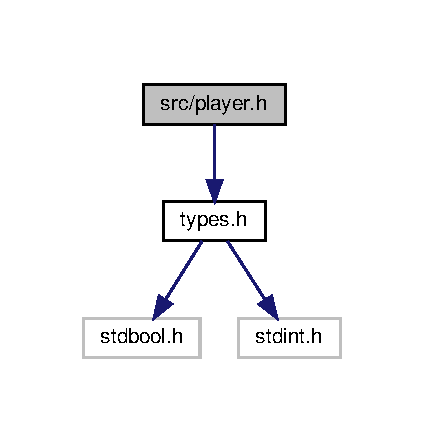
\includegraphics[width=204pt]{player_8h__incl}
\end{center}
\end{figure}
This graph shows which files directly or indirectly include this file\+:
\nopagebreak
\begin{figure}[H]
\begin{center}
\leavevmode
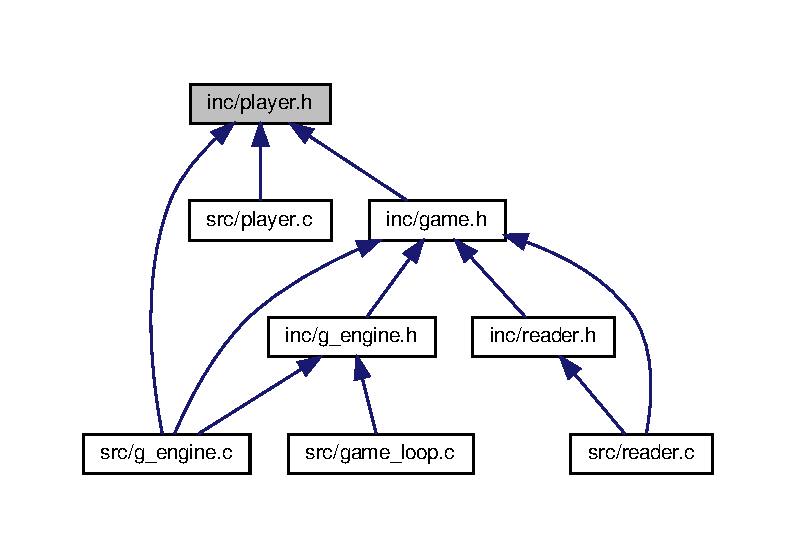
\includegraphics[width=251pt]{player_8h__dep__incl}
\end{center}
\end{figure}
\subsection*{Macros}
\begin{DoxyCompactItemize}
\item 
\mbox{\Hypertarget{player_8h_a1c346c944e8204fd06dc057393c7c96d}\label{player_8h_a1c346c944e8204fd06dc057393c7c96d}} 
\#define {\bfseries M\+A\+X\+\_\+\+P\+L\+A\+Y\+E\+RS}~100
\item 
\mbox{\Hypertarget{player_8h_a89f0201fca94cbc3ca0f5fbce851e7c9}\label{player_8h_a89f0201fca94cbc3ca0f5fbce851e7c9}} 
\#define {\bfseries F\+I\+R\+S\+T\+\_\+\+P\+L\+A\+Y\+ER}~1
\end{DoxyCompactItemize}
\subsection*{Typedefs}
\begin{DoxyCompactItemize}
\item 
\mbox{\Hypertarget{player_8h_af30e2030635a69690f85e48bc6ef202f}\label{player_8h_af30e2030635a69690f85e48bc6ef202f}} 
typedef struct \hyperlink{struct__Player}{\+\_\+\+Player} {\bfseries Player}
\end{DoxyCompactItemize}
\subsection*{Functions}
\begin{DoxyCompactItemize}
\item 
\hyperlink{struct__Player}{Player} $\ast$ \hyperlink{player_8h_aed0f40de36238a60267abf71c6720599}{player\+\_\+init} ()
\item 
S\+T\+A\+T\+US \hyperlink{player_8h_a68e324aa5064e27d0a2f38aafb6809ad}{player\+\_\+destroy} (\hyperlink{struct__Player}{Player} $\ast$player)
\item 
Id \hyperlink{player_8h_af5a101ec91427951c5875569a8709956}{player\+\_\+get\+\_\+id} (\hyperlink{struct__Player}{Player} $\ast$player)
\item 
void \hyperlink{player_8h_a278466eff9dd013babc5bdbd485f1da0}{player\+\_\+set\+\_\+id} (\hyperlink{struct__Player}{Player} $\ast$player, Id id)
\item 
S\+T\+A\+T\+US \hyperlink{player_8h_a6a30809f7775f5c2d3bef47d92769e59}{player\+\_\+set\+\_\+name} (\hyperlink{struct__Player}{Player} $\ast$player, char $\ast$name)
\item 
const char $\ast$ \hyperlink{player_8h_a6622c02be2fe230a5c0df66385a13ece}{player\+\_\+get\+\_\+name} (\hyperlink{struct__Player}{Player} $\ast$player)
\item 
S\+T\+A\+T\+US \hyperlink{player_8h_ac8ace1a1b6b11bc7f92a71a3922e4b83}{player\+\_\+set\+\_\+location} (\hyperlink{struct__Player}{Player} $\ast$player, Id id)
\item 
Id \hyperlink{player_8h_aa50ce77ab79af7166d749619fd60acfe}{player\+\_\+get\+\_\+location} (\hyperlink{struct__Player}{Player} $\ast$player)
\item 
S\+T\+A\+T\+US \hyperlink{player_8h_af5eacaf6a51631f28500d8127e761c1b}{player\+\_\+set\+\_\+object} (\hyperlink{struct__Player}{Player} $\ast$player, Id id)
\item 
bool \hyperlink{player_8h_a2e262401b9b2b77978b421917c13279d}{player\+\_\+has\+\_\+object} (\hyperlink{struct__Player}{Player} $\ast$player)
\item 
S\+T\+A\+T\+US \hyperlink{player_8h_aa0f2f8b4d1b63a60ef927d47aa45dbd1}{player\+\_\+print} (\hyperlink{struct__Player}{Player} $\ast$player)
\item 
Id \hyperlink{player_8h_a96e37051cdc1540e0dde770f6b713f39}{player\+\_\+get\+\_\+object} (\hyperlink{struct__Player}{Player} $\ast$player)
\end{DoxyCompactItemize}


\subsection{Detailed Description}
It defines a player. 

\begin{DoxyVersion}{Version}
1.\+0 
\end{DoxyVersion}
\begin{DoxyDate}{Date}
07/02/2019 
\end{DoxyDate}
\begin{DoxyCopyright}{Copyright}
G\+NU Public License 
\end{DoxyCopyright}


\subsection{Function Documentation}
\mbox{\Hypertarget{player_8h_aed0f40de36238a60267abf71c6720599}\label{player_8h_aed0f40de36238a60267abf71c6720599}} 
\index{player.\+h@{player.\+h}!player\+\_\+init@{player\+\_\+init}}
\index{player\+\_\+init@{player\+\_\+init}!player.\+h@{player.\+h}}
\subsubsection{\texorpdfstring{player\+\_\+init()}{player\_init()}}
{\footnotesize\ttfamily \hyperlink{struct__Player}{Player}$\ast$ player\+\_\+init (\begin{DoxyParamCaption}{ }\end{DoxyParamCaption})}

player\+\_\+create defines a new player.


\begin{DoxyParams}{Parameters}
{\em \{\}} & -\/ do not receive arguments; \\
\hline
\end{DoxyParams}
\begin{DoxyReturn}{Returns}
\{Player$\ast$\} -\/ returns a player pointer; 
\end{DoxyReturn}
\mbox{\Hypertarget{player_8h_a68e324aa5064e27d0a2f38aafb6809ad}\label{player_8h_a68e324aa5064e27d0a2f38aafb6809ad}} 
\index{player.\+h@{player.\+h}!player\+\_\+destroy@{player\+\_\+destroy}}
\index{player\+\_\+destroy@{player\+\_\+destroy}!player.\+h@{player.\+h}}
\subsubsection{\texorpdfstring{player\+\_\+destroy()}{player\_destroy()}}
{\footnotesize\ttfamily S\+T\+A\+T\+US player\+\_\+destroy (\begin{DoxyParamCaption}\item[{\hyperlink{struct__Player}{Player} $\ast$}]{player }\end{DoxyParamCaption})}

player\+\_\+destroy destroys a player.


\begin{DoxyParams}{Parameters}
{\em \{\+Player$\ast$\}} & -\/ player; \\
\hline
\end{DoxyParams}
\begin{DoxyReturn}{Returns}
\{S\+T\+A\+T\+US\} -\/ Returns a state; 
\end{DoxyReturn}
\mbox{\Hypertarget{player_8h_af5a101ec91427951c5875569a8709956}\label{player_8h_af5a101ec91427951c5875569a8709956}} 
\index{player.\+h@{player.\+h}!player\+\_\+get\+\_\+id@{player\+\_\+get\+\_\+id}}
\index{player\+\_\+get\+\_\+id@{player\+\_\+get\+\_\+id}!player.\+h@{player.\+h}}
\subsubsection{\texorpdfstring{player\+\_\+get\+\_\+id()}{player\_get\_id()}}
{\footnotesize\ttfamily Id player\+\_\+get\+\_\+id (\begin{DoxyParamCaption}\item[{\hyperlink{struct__Player}{Player} $\ast$}]{player }\end{DoxyParamCaption})}

player\+\_\+get\+\_\+id takes the id of a player.


\begin{DoxyParams}{Parameters}
{\em \{\+Player$\ast$\}} & -\/ player; \\
\hline
\end{DoxyParams}
\begin{DoxyReturn}{Returns}
\{Id\} -\/ Returns an id; 
\end{DoxyReturn}
\mbox{\Hypertarget{player_8h_a278466eff9dd013babc5bdbd485f1da0}\label{player_8h_a278466eff9dd013babc5bdbd485f1da0}} 
\index{player.\+h@{player.\+h}!player\+\_\+set\+\_\+id@{player\+\_\+set\+\_\+id}}
\index{player\+\_\+set\+\_\+id@{player\+\_\+set\+\_\+id}!player.\+h@{player.\+h}}
\subsubsection{\texorpdfstring{player\+\_\+set\+\_\+id()}{player\_set\_id()}}
{\footnotesize\ttfamily void player\+\_\+set\+\_\+id (\begin{DoxyParamCaption}\item[{\hyperlink{struct__Player}{Player} $\ast$}]{player,  }\item[{Id}]{id }\end{DoxyParamCaption})}

player\+\_\+set\+\_\+id sets te id of a player.


\begin{DoxyParams}{Parameters}
{\em \{\+Player$\ast$\}} & -\/ player; \{Id\} -\/ id; \\
\hline
\end{DoxyParams}
\begin{DoxyReturn}{Returns}
\{void\} -\/ Do not return nothing; 
\end{DoxyReturn}
\mbox{\Hypertarget{player_8h_a6a30809f7775f5c2d3bef47d92769e59}\label{player_8h_a6a30809f7775f5c2d3bef47d92769e59}} 
\index{player.\+h@{player.\+h}!player\+\_\+set\+\_\+name@{player\+\_\+set\+\_\+name}}
\index{player\+\_\+set\+\_\+name@{player\+\_\+set\+\_\+name}!player.\+h@{player.\+h}}
\subsubsection{\texorpdfstring{player\+\_\+set\+\_\+name()}{player\_set\_name()}}
{\footnotesize\ttfamily S\+T\+A\+T\+US player\+\_\+set\+\_\+name (\begin{DoxyParamCaption}\item[{\hyperlink{struct__Player}{Player} $\ast$}]{player,  }\item[{char $\ast$}]{name }\end{DoxyParamCaption})}

player\+\_\+set\+\_\+name defines the name of a player.


\begin{DoxyParams}{Parameters}
{\em \{\+Player$\ast$\}} & -\/ player; \{Char$\ast$\} -\/ name; \\
\hline
\end{DoxyParams}
\begin{DoxyReturn}{Returns}
\{S\+T\+A\+T\+US\} -\/ Returns an state; 
\end{DoxyReturn}
\mbox{\Hypertarget{player_8h_a6622c02be2fe230a5c0df66385a13ece}\label{player_8h_a6622c02be2fe230a5c0df66385a13ece}} 
\index{player.\+h@{player.\+h}!player\+\_\+get\+\_\+name@{player\+\_\+get\+\_\+name}}
\index{player\+\_\+get\+\_\+name@{player\+\_\+get\+\_\+name}!player.\+h@{player.\+h}}
\subsubsection{\texorpdfstring{player\+\_\+get\+\_\+name()}{player\_get\_name()}}
{\footnotesize\ttfamily const char$\ast$ player\+\_\+get\+\_\+name (\begin{DoxyParamCaption}\item[{\hyperlink{struct__Player}{Player} $\ast$}]{player }\end{DoxyParamCaption})}

player\+\_\+get\+\_\+name takes the name of a player.


\begin{DoxyParams}{Parameters}
{\em \{\+Player$\ast$\}} & -\/ player; \\
\hline
\end{DoxyParams}
\begin{DoxyReturn}{Returns}
\{const char$\ast$\} -\/ Returns a constant character array; 
\end{DoxyReturn}
\mbox{\Hypertarget{player_8h_ac8ace1a1b6b11bc7f92a71a3922e4b83}\label{player_8h_ac8ace1a1b6b11bc7f92a71a3922e4b83}} 
\index{player.\+h@{player.\+h}!player\+\_\+set\+\_\+location@{player\+\_\+set\+\_\+location}}
\index{player\+\_\+set\+\_\+location@{player\+\_\+set\+\_\+location}!player.\+h@{player.\+h}}
\subsubsection{\texorpdfstring{player\+\_\+set\+\_\+location()}{player\_set\_location()}}
{\footnotesize\ttfamily S\+T\+A\+T\+US player\+\_\+set\+\_\+location (\begin{DoxyParamCaption}\item[{\hyperlink{struct__Player}{Player} $\ast$}]{player,  }\item[{Id}]{id }\end{DoxyParamCaption})}

player\+\_\+set\+\_\+north sets the location of a player.


\begin{DoxyParams}{Parameters}
{\em \{\+Player$\ast$\}} & -\/ player; \{Id\} -\/ id; \\
\hline
\end{DoxyParams}
\begin{DoxyReturn}{Returns}
\{S\+T\+A\+T\+US\} -\/ Returns an state; 
\end{DoxyReturn}
\mbox{\Hypertarget{player_8h_aa50ce77ab79af7166d749619fd60acfe}\label{player_8h_aa50ce77ab79af7166d749619fd60acfe}} 
\index{player.\+h@{player.\+h}!player\+\_\+get\+\_\+location@{player\+\_\+get\+\_\+location}}
\index{player\+\_\+get\+\_\+location@{player\+\_\+get\+\_\+location}!player.\+h@{player.\+h}}
\subsubsection{\texorpdfstring{player\+\_\+get\+\_\+location()}{player\_get\_location()}}
{\footnotesize\ttfamily Id player\+\_\+get\+\_\+location (\begin{DoxyParamCaption}\item[{\hyperlink{struct__Player}{Player} $\ast$}]{player }\end{DoxyParamCaption})}

player\+\_\+get\+\_\+north gets the location of a players.


\begin{DoxyParams}{Parameters}
{\em \{\+Player$\ast$\}} & -\/ player; \\
\hline
\end{DoxyParams}
\begin{DoxyReturn}{Returns}
\{Id\} -\/ Returns an id; 
\end{DoxyReturn}
\mbox{\Hypertarget{player_8h_af5eacaf6a51631f28500d8127e761c1b}\label{player_8h_af5eacaf6a51631f28500d8127e761c1b}} 
\index{player.\+h@{player.\+h}!player\+\_\+set\+\_\+object@{player\+\_\+set\+\_\+object}}
\index{player\+\_\+set\+\_\+object@{player\+\_\+set\+\_\+object}!player.\+h@{player.\+h}}
\subsubsection{\texorpdfstring{player\+\_\+set\+\_\+object()}{player\_set\_object()}}
{\footnotesize\ttfamily S\+T\+A\+T\+US player\+\_\+set\+\_\+object (\begin{DoxyParamCaption}\item[{\hyperlink{struct__Player}{Player} $\ast$}]{player,  }\item[{Id}]{id }\end{DoxyParamCaption})}

player\+\_\+set\+\_\+object sets an id to a player\textquotesingle{}s object.


\begin{DoxyParams}{Parameters}
{\em \{\+Player$\ast$\}} & -\/ player; \{Id\} -\/ id; \\
\hline
\end{DoxyParams}
\begin{DoxyReturn}{Returns}
\{S\+T\+A\+T\+US\} -\/ Returns an state; 
\end{DoxyReturn}
\mbox{\Hypertarget{player_8h_a2e262401b9b2b77978b421917c13279d}\label{player_8h_a2e262401b9b2b77978b421917c13279d}} 
\index{player.\+h@{player.\+h}!player\+\_\+has\+\_\+object@{player\+\_\+has\+\_\+object}}
\index{player\+\_\+has\+\_\+object@{player\+\_\+has\+\_\+object}!player.\+h@{player.\+h}}
\subsubsection{\texorpdfstring{player\+\_\+has\+\_\+object()}{player\_has\_object()}}
{\footnotesize\ttfamily bool player\+\_\+has\+\_\+object (\begin{DoxyParamCaption}\item[{\hyperlink{struct__Player}{Player} $\ast$}]{player }\end{DoxyParamCaption})}

player\+\_\+has\+\_\+object gets a pointer towards an object.


\begin{DoxyParams}{Parameters}
{\em \{\+Game$\ast$\}} & -\/ game; \\
\hline
\end{DoxyParams}
\begin{DoxyReturn}{Returns}
\{void\} -\/ Do not returns nothing; 
\end{DoxyReturn}
\mbox{\Hypertarget{player_8h_aa0f2f8b4d1b63a60ef927d47aa45dbd1}\label{player_8h_aa0f2f8b4d1b63a60ef927d47aa45dbd1}} 
\index{player.\+h@{player.\+h}!player\+\_\+print@{player\+\_\+print}}
\index{player\+\_\+print@{player\+\_\+print}!player.\+h@{player.\+h}}
\subsubsection{\texorpdfstring{player\+\_\+print()}{player\_print()}}
{\footnotesize\ttfamily S\+T\+A\+T\+US player\+\_\+print (\begin{DoxyParamCaption}\item[{\hyperlink{struct__Player}{Player} $\ast$}]{player }\end{DoxyParamCaption})}

player\+\_\+print prints a player on the game screen.


\begin{DoxyParams}{Parameters}
{\em \{\+Game$\ast$\}} & -\/ game; \\
\hline
\end{DoxyParams}
\begin{DoxyReturn}{Returns}
\{void\} -\/ Do not returns nothing; 
\end{DoxyReturn}
\mbox{\Hypertarget{player_8h_a96e37051cdc1540e0dde770f6b713f39}\label{player_8h_a96e37051cdc1540e0dde770f6b713f39}} 
\index{player.\+h@{player.\+h}!player\+\_\+get\+\_\+object@{player\+\_\+get\+\_\+object}}
\index{player\+\_\+get\+\_\+object@{player\+\_\+get\+\_\+object}!player.\+h@{player.\+h}}
\subsubsection{\texorpdfstring{player\+\_\+get\+\_\+object()}{player\_get\_object()}}
{\footnotesize\ttfamily Id player\+\_\+get\+\_\+object (\begin{DoxyParamCaption}\item[{\hyperlink{struct__Player}{Player} $\ast$}]{player }\end{DoxyParamCaption})}

player\+\_\+get\+\_\+object gets the id of a player\textquotesingle{}s object.


\begin{DoxyParams}{Parameters}
{\em \{\+Player$\ast$\}} & -\/ player; \\
\hline
\end{DoxyParams}
\begin{DoxyReturn}{Returns}
\{Id\} -\/ Returns id; 
\end{DoxyReturn}

\hypertarget{reader_8h}{}\section{inc/reader.h File Reference}
\label{reader_8h}\index{inc/reader.\+h@{inc/reader.\+h}}


Defines a game reader.  


{\ttfamily \#include \char`\"{}game.\+h\char`\"{}}\newline
Include dependency graph for reader.\+h\+:\nopagebreak
\begin{figure}[H]
\begin{center}
\leavevmode
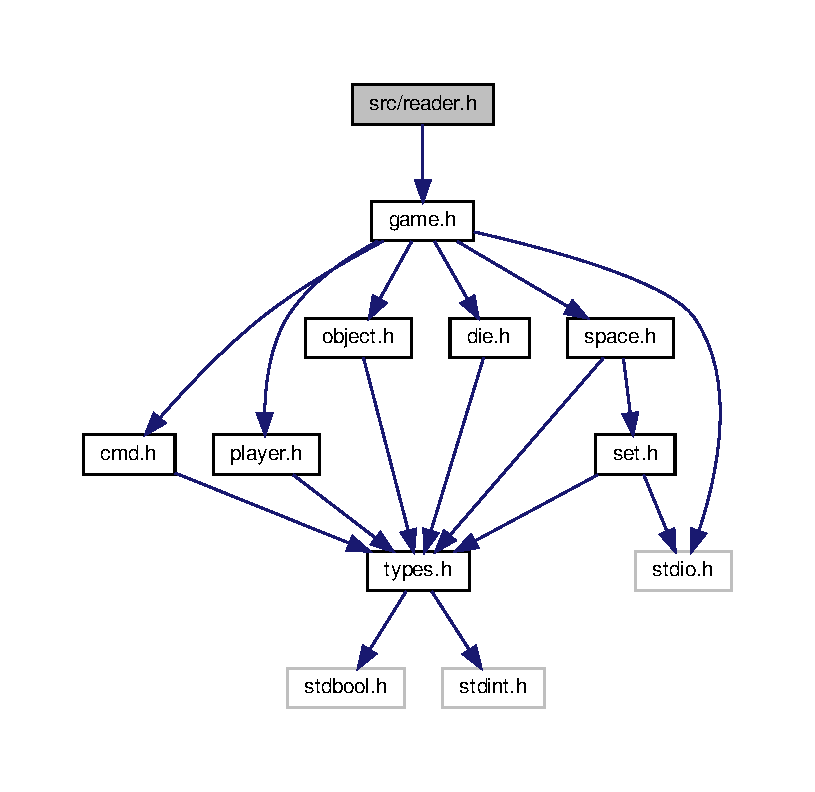
\includegraphics[width=350pt]{reader_8h__incl}
\end{center}
\end{figure}
This graph shows which files directly or indirectly include this file\+:
\nopagebreak
\begin{figure}[H]
\begin{center}
\leavevmode
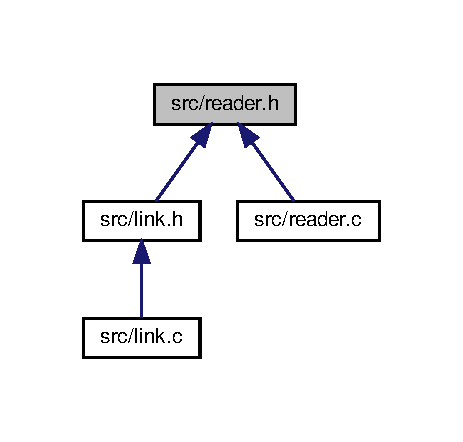
\includegraphics[width=148pt]{reader_8h__dep__incl}
\end{center}
\end{figure}
\subsection*{Functions}
\begin{DoxyCompactItemize}
\item 
\hyperlink{types_8h_a32c27cc471df37f4fc818d65de0a56c4}{S\+T\+A\+T\+US} \hyperlink{reader_8h_a06b7c64080352bc7659460735c0e93be}{reader\+\_\+load\+\_\+links} (\hyperlink{struct__Game}{Game} $\ast$game, char $\ast$f\+\_\+name)
\begin{DoxyCompactList}\small\item\em Loads links from a file. \end{DoxyCompactList}\item 
\hyperlink{types_8h_a32c27cc471df37f4fc818d65de0a56c4}{S\+T\+A\+T\+US} \hyperlink{reader_8h_a329b3f09b9f244887808b807a33457c8}{reader\+\_\+load\+\_\+spaces} (\hyperlink{struct__Game}{Game} $\ast$game, char $\ast$f\+\_\+name)
\begin{DoxyCompactList}\small\item\em Loads spaces from a file. \end{DoxyCompactList}\item 
\hyperlink{types_8h_a32c27cc471df37f4fc818d65de0a56c4}{S\+T\+A\+T\+US} \hyperlink{reader_8h_ab8bed1641bb108e505b372bfb23a6604}{reader\+\_\+load\+\_\+objects} (\hyperlink{struct__Game}{Game} $\ast$game, char $\ast$f\+\_\+name)
\begin{DoxyCompactList}\small\item\em Loads objects from a file. \end{DoxyCompactList}\end{DoxyCompactItemize}


\subsection{Detailed Description}
Defines a game reader. 

Contains the implementation of the functions that are associated to the reading of the file To obtain its values

\begin{DoxyVersion}{Version}
1.\+0 
\end{DoxyVersion}
\begin{DoxyDate}{Date}
07/02/2019 
\end{DoxyDate}
\begin{DoxyAuthor}{Author}
Álvaro Rodríguez 
\end{DoxyAuthor}
\begin{DoxyCopyright}{Copyright}
G\+NU Public License 
\end{DoxyCopyright}


\subsection{Function Documentation}
\mbox{\Hypertarget{reader_8h_a06b7c64080352bc7659460735c0e93be}\label{reader_8h_a06b7c64080352bc7659460735c0e93be}} 
\index{reader.\+h@{reader.\+h}!reader\+\_\+load\+\_\+links@{reader\+\_\+load\+\_\+links}}
\index{reader\+\_\+load\+\_\+links@{reader\+\_\+load\+\_\+links}!reader.\+h@{reader.\+h}}
\subsubsection{\texorpdfstring{reader\+\_\+load\+\_\+links()}{reader\_load\_links()}}
{\footnotesize\ttfamily \hyperlink{types_8h_a32c27cc471df37f4fc818d65de0a56c4}{S\+T\+A\+T\+US} reader\+\_\+load\+\_\+links (\begin{DoxyParamCaption}\item[{\hyperlink{struct__Game}{Game} $\ast$}]{game,  }\item[{char $\ast$}]{f\+\_\+name }\end{DoxyParamCaption})}



Loads links from a file. 

\begin{DoxyDate}{Date}
07/02/2019 
\end{DoxyDate}
\begin{DoxyAuthor}{Author}
Javier Romera
\end{DoxyAuthor}

\begin{DoxyParams}{Parameters}
{\em \{\+Game$\ast$\}} & game -\/ Pointer to game data \\
\hline
{\em \{char$\ast$\}} & f\+\_\+name -\/ name of the source file \\
\hline
\end{DoxyParams}

\begin{DoxyRetVals}{Return values}
{\em \{\+S\+T\+A\+T\+U\+S\}} & -\/ Returns an status \\
\hline
\end{DoxyRetVals}
\mbox{\Hypertarget{reader_8h_a329b3f09b9f244887808b807a33457c8}\label{reader_8h_a329b3f09b9f244887808b807a33457c8}} 
\index{reader.\+h@{reader.\+h}!reader\+\_\+load\+\_\+spaces@{reader\+\_\+load\+\_\+spaces}}
\index{reader\+\_\+load\+\_\+spaces@{reader\+\_\+load\+\_\+spaces}!reader.\+h@{reader.\+h}}
\subsubsection{\texorpdfstring{reader\+\_\+load\+\_\+spaces()}{reader\_load\_spaces()}}
{\footnotesize\ttfamily \hyperlink{types_8h_a32c27cc471df37f4fc818d65de0a56c4}{S\+T\+A\+T\+US} reader\+\_\+load\+\_\+spaces (\begin{DoxyParamCaption}\item[{\hyperlink{struct__Game}{Game} $\ast$}]{game,  }\item[{char $\ast$}]{f\+\_\+name }\end{DoxyParamCaption})}



Loads spaces from a file. 

\begin{DoxyDate}{Date}
07/02/2019 
\end{DoxyDate}
\begin{DoxyAuthor}{Author}
Álvaro Rodríguez
\end{DoxyAuthor}

\begin{DoxyParams}{Parameters}
{\em \{\+Game$\ast$\}} & game -\/ Pointer to game data \\
\hline
{\em \{char$\ast$\}} & f\+\_\+name -\/ name of the source file \\
\hline
\end{DoxyParams}

\begin{DoxyRetVals}{Return values}
{\em \{\+S\+T\+A\+T\+U\+S\}} & -\/ Returns an status \\
\hline
\end{DoxyRetVals}
\mbox{\Hypertarget{reader_8h_ab8bed1641bb108e505b372bfb23a6604}\label{reader_8h_ab8bed1641bb108e505b372bfb23a6604}} 
\index{reader.\+h@{reader.\+h}!reader\+\_\+load\+\_\+objects@{reader\+\_\+load\+\_\+objects}}
\index{reader\+\_\+load\+\_\+objects@{reader\+\_\+load\+\_\+objects}!reader.\+h@{reader.\+h}}
\subsubsection{\texorpdfstring{reader\+\_\+load\+\_\+objects()}{reader\_load\_objects()}}
{\footnotesize\ttfamily \hyperlink{types_8h_a32c27cc471df37f4fc818d65de0a56c4}{S\+T\+A\+T\+US} reader\+\_\+load\+\_\+objects (\begin{DoxyParamCaption}\item[{\hyperlink{struct__Game}{Game} $\ast$}]{game,  }\item[{char $\ast$}]{f\+\_\+name }\end{DoxyParamCaption})}



Loads objects from a file. 

\begin{DoxyDate}{Date}
07/02/2019 
\end{DoxyDate}
\begin{DoxyAuthor}{Author}
Álvaro Rodríguez
\end{DoxyAuthor}

\begin{DoxyParams}{Parameters}
{\em \{\+Game$\ast$\}} & game -\/ Pointer to game data  \{char$\ast$\} filename -\/ name of the source file \\
\hline
\end{DoxyParams}

\begin{DoxyRetVals}{Return values}
{\em \{\+S\+T\+A\+T\+U\+S\}} & -\/ Returns an status \\
\hline
\end{DoxyRetVals}

\hypertarget{set_8h}{}\section{src/set.h File Reference}
\label{set_8h}\index{src/set.\+h@{src/set.\+h}}


It defines the set interface.  


{\ttfamily \#include $<$stdio.\+h$>$}\newline
{\ttfamily \#include \char`\"{}types.\+h\char`\"{}}\newline
Include dependency graph for set.\+h\+:\nopagebreak
\begin{figure}[H]
\begin{center}
\leavevmode
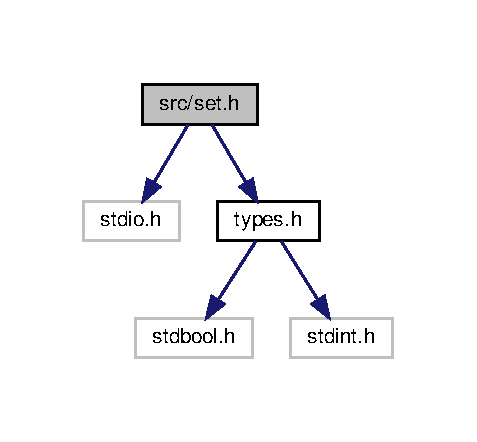
\includegraphics[width=229pt]{set_8h__incl}
\end{center}
\end{figure}
This graph shows which files directly or indirectly include this file\+:
\nopagebreak
\begin{figure}[H]
\begin{center}
\leavevmode
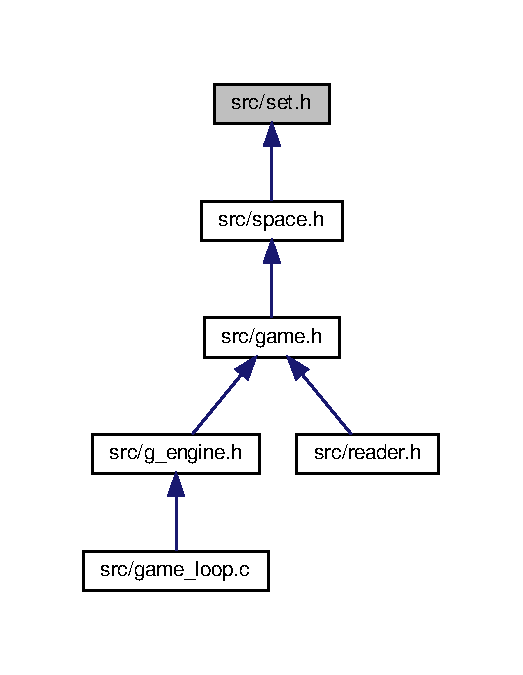
\includegraphics[width=350pt]{set_8h__dep__incl}
\end{center}
\end{figure}
\subsection*{Macros}
\begin{DoxyCompactItemize}
\item 
\mbox{\Hypertarget{set_8h_abc21882f4958e6b56aaf2f3c18f80d43}\label{set_8h_abc21882f4958e6b56aaf2f3c18f80d43}} 
\#define \hyperlink{set_8h_abc21882f4958e6b56aaf2f3c18f80d43}{M\+A\+X\+\_\+\+S\+ET}~5
\begin{DoxyCompactList}\small\item\em Maximum number of sets. \end{DoxyCompactList}\end{DoxyCompactItemize}
\subsection*{Typedefs}
\begin{DoxyCompactItemize}
\item 
\mbox{\Hypertarget{set_8h_a6d3b7f7c92cbb4577ef3ef7ddbf93161}\label{set_8h_a6d3b7f7c92cbb4577ef3ef7ddbf93161}} 
typedef struct \hyperlink{struct__Set}{\+\_\+\+Set} \hyperlink{set_8h_a6d3b7f7c92cbb4577ef3ef7ddbf93161}{Set}
\begin{DoxyCompactList}\small\item\em Definition of Set structure. \end{DoxyCompactList}\end{DoxyCompactItemize}
\subsection*{Functions}
\begin{DoxyCompactItemize}
\item 
\hyperlink{set_8h_a6d3b7f7c92cbb4577ef3ef7ddbf93161}{Set} $\ast$ \hyperlink{set_8h_abcc73b7ad3913fc92dd95d366c9c8687}{set\+\_\+create} ()
\begin{DoxyCompactList}\small\item\em Initializates a set of objets. \end{DoxyCompactList}\item 
void \hyperlink{set_8h_a9d762a027f1c3bcdd22f70ee9093a7dd}{set\+\_\+destroy} (\hyperlink{set_8h_a6d3b7f7c92cbb4577ef3ef7ddbf93161}{Set} $\ast$set)
\begin{DoxyCompactList}\small\item\em Destroys a set. \end{DoxyCompactList}\item 
\hyperlink{types_8h_a32c27cc471df37f4fc818d65de0a56c4}{S\+T\+A\+T\+US} \hyperlink{set_8h_af5e2395ece6e4c771f92a09039e20c48}{set\+\_\+add\+\_\+id} (\hyperlink{set_8h_a6d3b7f7c92cbb4577ef3ef7ddbf93161}{Set} $\ast$set, \hyperlink{types_8h_a845e604fb28f7e3d97549da3448149d3}{Id} id)
\begin{DoxyCompactList}\small\item\em Adds a new id to a set. \end{DoxyCompactList}\item 
\hyperlink{types_8h_a32c27cc471df37f4fc818d65de0a56c4}{S\+T\+A\+T\+US} \hyperlink{set_8h_abcd3b47d23dc810bdf9c95cee08657f8}{set\+\_\+del\+\_\+id} (\hyperlink{set_8h_a6d3b7f7c92cbb4577ef3ef7ddbf93161}{Set} $\ast$set, \hyperlink{types_8h_a845e604fb28f7e3d97549da3448149d3}{Id} id)
\begin{DoxyCompactList}\small\item\em Deletes an id from a set. \end{DoxyCompactList}\item 
bool \hyperlink{set_8h_a6f711461ca39891dd255f69fda0dac63}{set\+\_\+has\+\_\+id} (\hyperlink{set_8h_a6d3b7f7c92cbb4577ef3ef7ddbf93161}{Set} $\ast$set, \hyperlink{types_8h_a845e604fb28f7e3d97549da3448149d3}{Id} id)
\begin{DoxyCompactList}\small\item\em Tells if an id is in a set or not. \end{DoxyCompactList}\item 
int \hyperlink{set_8h_af7ef2f473f47ce1ea8cfc2c3d38f06ef}{set\+\_\+get\+\_\+total} (\hyperlink{set_8h_a6d3b7f7c92cbb4577ef3ef7ddbf93161}{Set} $\ast$set)
\begin{DoxyCompactList}\small\item\em Tells the number of id\textquotesingle{}s in a set. \end{DoxyCompactList}\item 
bool \hyperlink{set_8h_acfcaddd02eb2182e51853316a47b277b}{set\+\_\+is\+\_\+full} (\hyperlink{set_8h_a6d3b7f7c92cbb4577ef3ef7ddbf93161}{Set} $\ast$set)
\begin{DoxyCompactList}\small\item\em Tells if a set is full or not. \end{DoxyCompactList}\item 
bool \hyperlink{set_8h_a708ba2be9a85217a7fe47705b11136d1}{set\+\_\+is\+\_\+empty} (\hyperlink{set_8h_a6d3b7f7c92cbb4577ef3ef7ddbf93161}{Set} $\ast$set)
\begin{DoxyCompactList}\small\item\em Tells if a set is empty or not. \end{DoxyCompactList}\item 
\hyperlink{types_8h_a845e604fb28f7e3d97549da3448149d3}{Id} \hyperlink{set_8h_af299dc4d834e837a9530858608c165dd}{set\+\_\+get\+\_\+first} (\hyperlink{set_8h_a6d3b7f7c92cbb4577ef3ef7ddbf93161}{Set} $\ast$set)
\begin{DoxyCompactList}\small\item\em Gets the first Id of a set, just for testing. \end{DoxyCompactList}\item 
int \hyperlink{set_8h_a4a2be47265517919b4d98b9e209c578e}{set\+\_\+print} (F\+I\+LE $\ast$stream, \hyperlink{set_8h_a6d3b7f7c92cbb4577ef3ef7ddbf93161}{Set} $\ast$set)
\begin{DoxyCompactList}\small\item\em Prints a set. \end{DoxyCompactList}\end{DoxyCompactItemize}


\subsection{Detailed Description}
It defines the set interface. 

\begin{DoxyVersion}{Version}
0.\+3.\+2 
\end{DoxyVersion}
\begin{DoxyDate}{Date}
19/03/2019 
\end{DoxyDate}
\begin{DoxyCopyright}{Copyright}
G\+NU Public License 
\end{DoxyCopyright}


\subsection{Function Documentation}
\mbox{\Hypertarget{set_8h_abcc73b7ad3913fc92dd95d366c9c8687}\label{set_8h_abcc73b7ad3913fc92dd95d366c9c8687}} 
\index{set.\+h@{set.\+h}!set\+\_\+create@{set\+\_\+create}}
\index{set\+\_\+create@{set\+\_\+create}!set.\+h@{set.\+h}}
\subsubsection{\texorpdfstring{set\+\_\+create()}{set\_create()}}
{\footnotesize\ttfamily \hyperlink{set_8h_a6d3b7f7c92cbb4577ef3ef7ddbf93161}{Set}$\ast$ set\+\_\+create (\begin{DoxyParamCaption}{ }\end{DoxyParamCaption})}



Initializates a set of objets. 

\begin{DoxyAuthor}{Author}
Álvaro Rodríguez 
\end{DoxyAuthor}

\begin{DoxyRetVals}{Return values}
{\em Returns} & a pointer towards a new set \\
\hline
\end{DoxyRetVals}
\mbox{\Hypertarget{set_8h_a9d762a027f1c3bcdd22f70ee9093a7dd}\label{set_8h_a9d762a027f1c3bcdd22f70ee9093a7dd}} 
\index{set.\+h@{set.\+h}!set\+\_\+destroy@{set\+\_\+destroy}}
\index{set\+\_\+destroy@{set\+\_\+destroy}!set.\+h@{set.\+h}}
\subsubsection{\texorpdfstring{set\+\_\+destroy()}{set\_destroy()}}
{\footnotesize\ttfamily void set\+\_\+destroy (\begin{DoxyParamCaption}\item[{\hyperlink{set_8h_a6d3b7f7c92cbb4577ef3ef7ddbf93161}{Set} $\ast$}]{set }\end{DoxyParamCaption})}



Destroys a set. 

\begin{DoxyAuthor}{Author}
Álvaro Rodríguez 
\end{DoxyAuthor}

\begin{DoxyParams}{Parameters}
{\em \{\+Set$\ast$\}} & -\/ Receives a set which is going to be freed \\
\hline
\end{DoxyParams}
\mbox{\Hypertarget{set_8h_af5e2395ece6e4c771f92a09039e20c48}\label{set_8h_af5e2395ece6e4c771f92a09039e20c48}} 
\index{set.\+h@{set.\+h}!set\+\_\+add\+\_\+id@{set\+\_\+add\+\_\+id}}
\index{set\+\_\+add\+\_\+id@{set\+\_\+add\+\_\+id}!set.\+h@{set.\+h}}
\subsubsection{\texorpdfstring{set\+\_\+add\+\_\+id()}{set\_add\_id()}}
{\footnotesize\ttfamily \hyperlink{types_8h_a32c27cc471df37f4fc818d65de0a56c4}{S\+T\+A\+T\+US} set\+\_\+add\+\_\+id (\begin{DoxyParamCaption}\item[{\hyperlink{set_8h_a6d3b7f7c92cbb4577ef3ef7ddbf93161}{Set} $\ast$}]{set,  }\item[{\hyperlink{types_8h_a845e604fb28f7e3d97549da3448149d3}{Id}}]{id }\end{DoxyParamCaption})}



Adds a new id to a set. 

\begin{DoxyAuthor}{Author}
Álvaro Rodríguez 
\end{DoxyAuthor}

\begin{DoxyParams}{Parameters}
{\em \{\+Set$\ast$\}} & -\/ Receives a set which is going to be freed \\
\hline
\end{DoxyParams}

\begin{DoxyRetVals}{Return values}
{\em \{\+S\+T\+A\+T\+U\+S\}} & -\/ Returns ok or error \\
\hline
\end{DoxyRetVals}
\mbox{\Hypertarget{set_8h_abcd3b47d23dc810bdf9c95cee08657f8}\label{set_8h_abcd3b47d23dc810bdf9c95cee08657f8}} 
\index{set.\+h@{set.\+h}!set\+\_\+del\+\_\+id@{set\+\_\+del\+\_\+id}}
\index{set\+\_\+del\+\_\+id@{set\+\_\+del\+\_\+id}!set.\+h@{set.\+h}}
\subsubsection{\texorpdfstring{set\+\_\+del\+\_\+id()}{set\_del\_id()}}
{\footnotesize\ttfamily \hyperlink{types_8h_a32c27cc471df37f4fc818d65de0a56c4}{S\+T\+A\+T\+US} set\+\_\+del\+\_\+id (\begin{DoxyParamCaption}\item[{\hyperlink{set_8h_a6d3b7f7c92cbb4577ef3ef7ddbf93161}{Set} $\ast$}]{set,  }\item[{\hyperlink{types_8h_a845e604fb28f7e3d97549da3448149d3}{Id}}]{id }\end{DoxyParamCaption})}



Deletes an id from a set. 

\begin{DoxyAuthor}{Author}
Álvaro Rodríguez 
\end{DoxyAuthor}

\begin{DoxyParams}{Parameters}
{\em \{\+Set$\ast$\}} & -\/ Receives a set which is going to be freed \\
\hline
\end{DoxyParams}

\begin{DoxyRetVals}{Return values}
{\em \{\+S\+T\+A\+T\+U\+S\}} & -\/ Returns ok or error \\
\hline
\end{DoxyRetVals}
\mbox{\Hypertarget{set_8h_a6f711461ca39891dd255f69fda0dac63}\label{set_8h_a6f711461ca39891dd255f69fda0dac63}} 
\index{set.\+h@{set.\+h}!set\+\_\+has\+\_\+id@{set\+\_\+has\+\_\+id}}
\index{set\+\_\+has\+\_\+id@{set\+\_\+has\+\_\+id}!set.\+h@{set.\+h}}
\subsubsection{\texorpdfstring{set\+\_\+has\+\_\+id()}{set\_has\_id()}}
{\footnotesize\ttfamily bool set\+\_\+has\+\_\+id (\begin{DoxyParamCaption}\item[{\hyperlink{set_8h_a6d3b7f7c92cbb4577ef3ef7ddbf93161}{Set} $\ast$}]{set,  }\item[{\hyperlink{types_8h_a845e604fb28f7e3d97549da3448149d3}{Id}}]{id }\end{DoxyParamCaption})}



Tells if an id is in a set or not. 

\begin{DoxyAuthor}{Author}
Álvaro Rodríguez 
\end{DoxyAuthor}

\begin{DoxyParams}{Parameters}
{\em \{\+Set$\ast$\}} & -\/ Receives a set which is going to be freed \\
\hline
\end{DoxyParams}

\begin{DoxyRetVals}{Return values}
{\em \{bool\}} & -\/ Returns a boolean value \\
\hline
\end{DoxyRetVals}
\mbox{\Hypertarget{set_8h_af7ef2f473f47ce1ea8cfc2c3d38f06ef}\label{set_8h_af7ef2f473f47ce1ea8cfc2c3d38f06ef}} 
\index{set.\+h@{set.\+h}!set\+\_\+get\+\_\+total@{set\+\_\+get\+\_\+total}}
\index{set\+\_\+get\+\_\+total@{set\+\_\+get\+\_\+total}!set.\+h@{set.\+h}}
\subsubsection{\texorpdfstring{set\+\_\+get\+\_\+total()}{set\_get\_total()}}
{\footnotesize\ttfamily int set\+\_\+get\+\_\+total (\begin{DoxyParamCaption}\item[{\hyperlink{set_8h_a6d3b7f7c92cbb4577ef3ef7ddbf93161}{Set} $\ast$}]{set }\end{DoxyParamCaption})}



Tells the number of id\textquotesingle{}s in a set. 

\begin{DoxyAuthor}{Author}
Álvaro Rodríguez 
\end{DoxyAuthor}

\begin{DoxyParams}{Parameters}
{\em \{\+Set$\ast$\}} & -\/ Receives a set which is going to be freed \\
\hline
\end{DoxyParams}

\begin{DoxyRetVals}{Return values}
{\em \{int\}} & -\/ Returns an integer \\
\hline
\end{DoxyRetVals}
\mbox{\Hypertarget{set_8h_acfcaddd02eb2182e51853316a47b277b}\label{set_8h_acfcaddd02eb2182e51853316a47b277b}} 
\index{set.\+h@{set.\+h}!set\+\_\+is\+\_\+full@{set\+\_\+is\+\_\+full}}
\index{set\+\_\+is\+\_\+full@{set\+\_\+is\+\_\+full}!set.\+h@{set.\+h}}
\subsubsection{\texorpdfstring{set\+\_\+is\+\_\+full()}{set\_is\_full()}}
{\footnotesize\ttfamily bool set\+\_\+is\+\_\+full (\begin{DoxyParamCaption}\item[{\hyperlink{set_8h_a6d3b7f7c92cbb4577ef3ef7ddbf93161}{Set} $\ast$}]{set }\end{DoxyParamCaption})}



Tells if a set is full or not. 

\begin{DoxyAuthor}{Author}
Álvaro Rodríguez 
\end{DoxyAuthor}

\begin{DoxyParams}{Parameters}
{\em \{\+Set$\ast$\}} & -\/ Receives a set which is going to be freed \\
\hline
\end{DoxyParams}

\begin{DoxyRetVals}{Return values}
{\em \{bool\}} & -\/ Returns a boolean value \\
\hline
\end{DoxyRetVals}
\mbox{\Hypertarget{set_8h_a708ba2be9a85217a7fe47705b11136d1}\label{set_8h_a708ba2be9a85217a7fe47705b11136d1}} 
\index{set.\+h@{set.\+h}!set\+\_\+is\+\_\+empty@{set\+\_\+is\+\_\+empty}}
\index{set\+\_\+is\+\_\+empty@{set\+\_\+is\+\_\+empty}!set.\+h@{set.\+h}}
\subsubsection{\texorpdfstring{set\+\_\+is\+\_\+empty()}{set\_is\_empty()}}
{\footnotesize\ttfamily bool set\+\_\+is\+\_\+empty (\begin{DoxyParamCaption}\item[{\hyperlink{set_8h_a6d3b7f7c92cbb4577ef3ef7ddbf93161}{Set} $\ast$}]{set }\end{DoxyParamCaption})}



Tells if a set is empty or not. 

\begin{DoxyAuthor}{Author}
Álvaro Rodríguez 
\end{DoxyAuthor}

\begin{DoxyParams}{Parameters}
{\em \{\+Set$\ast$\}} & -\/ Receives a set which is going to be freed \\
\hline
\end{DoxyParams}

\begin{DoxyRetVals}{Return values}
{\em \{bool\}} & -\/ Returns ok or error \\
\hline
\end{DoxyRetVals}
\mbox{\Hypertarget{set_8h_af299dc4d834e837a9530858608c165dd}\label{set_8h_af299dc4d834e837a9530858608c165dd}} 
\index{set.\+h@{set.\+h}!set\+\_\+get\+\_\+first@{set\+\_\+get\+\_\+first}}
\index{set\+\_\+get\+\_\+first@{set\+\_\+get\+\_\+first}!set.\+h@{set.\+h}}
\subsubsection{\texorpdfstring{set\+\_\+get\+\_\+first()}{set\_get\_first()}}
{\footnotesize\ttfamily \hyperlink{types_8h_a845e604fb28f7e3d97549da3448149d3}{Id} set\+\_\+get\+\_\+first (\begin{DoxyParamCaption}\item[{\hyperlink{set_8h_a6d3b7f7c92cbb4577ef3ef7ddbf93161}{Set} $\ast$}]{set }\end{DoxyParamCaption})}



Gets the first Id of a set, just for testing. 

\begin{DoxyAuthor}{Author}
Javier Romera 
\end{DoxyAuthor}

\begin{DoxyParams}{Parameters}
{\em \{\+Set$\ast$\}} & -\/ Receives a set \\
\hline
\end{DoxyParams}

\begin{DoxyRetVals}{Return values}
{\em \{\+Id\}} & -\/ Returns a Id \\
\hline
\end{DoxyRetVals}
\mbox{\Hypertarget{set_8h_a4a2be47265517919b4d98b9e209c578e}\label{set_8h_a4a2be47265517919b4d98b9e209c578e}} 
\index{set.\+h@{set.\+h}!set\+\_\+print@{set\+\_\+print}}
\index{set\+\_\+print@{set\+\_\+print}!set.\+h@{set.\+h}}
\subsubsection{\texorpdfstring{set\+\_\+print()}{set\_print()}}
{\footnotesize\ttfamily int set\+\_\+print (\begin{DoxyParamCaption}\item[{F\+I\+LE $\ast$}]{stream,  }\item[{\hyperlink{set_8h_a6d3b7f7c92cbb4577ef3ef7ddbf93161}{Set} $\ast$}]{set }\end{DoxyParamCaption})}



Prints a set. 

\begin{DoxyAuthor}{Author}
Álvaro Rodríguez 
\end{DoxyAuthor}

\begin{DoxyParams}{Parameters}
{\em \{\+Set$\ast$\}} & -\/ Receives a set which is going to be freed \\
\hline
\end{DoxyParams}

\begin{DoxyRetVals}{Return values}
{\em \{int\}} & -\/ Returns an integer which contains the number of bytes \\
\hline
\end{DoxyRetVals}

\hypertarget{space_8h}{}\section{src/space.h File Reference}
\label{space_8h}\index{src/space.\+h@{src/space.\+h}}


Space module.  


{\ttfamily \#include \char`\"{}types.\+h\char`\"{}}\newline
{\ttfamily \#include \char`\"{}set.\+h\char`\"{}}\newline
Include dependency graph for space.\+h\+:\nopagebreak
\begin{figure}[H]
\begin{center}
\leavevmode
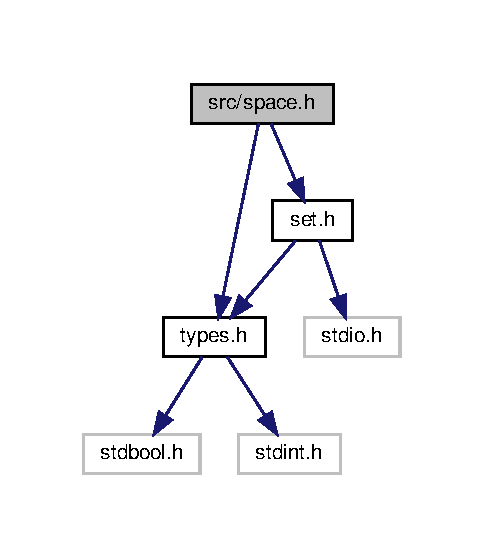
\includegraphics[width=232pt]{space_8h__incl}
\end{center}
\end{figure}
This graph shows which files directly or indirectly include this file\+:\nopagebreak
\begin{figure}[H]
\begin{center}
\leavevmode
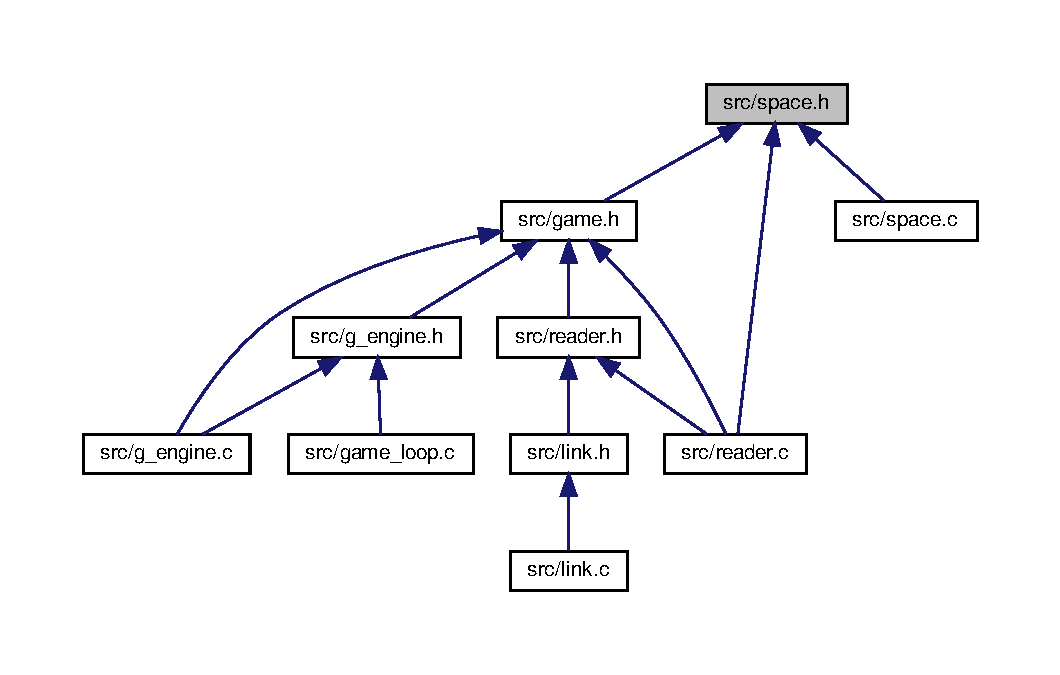
\includegraphics[width=314pt]{space_8h__dep__incl}
\end{center}
\end{figure}
\subsection*{Macros}
\begin{DoxyCompactItemize}
\item 
\mbox{\Hypertarget{space_8h_a5f54fd55f983a2e33ce076cd9f587e82}\label{space_8h_a5f54fd55f983a2e33ce076cd9f587e82}} 
\#define {\bfseries M\+A\+X\+\_\+\+S\+P\+A\+C\+ES}~200
\item 
\mbox{\Hypertarget{space_8h_a088cbe7c6f78264d46c2624194c5c680}\label{space_8h_a088cbe7c6f78264d46c2624194c5c680}} 
\#define {\bfseries F\+I\+R\+S\+T\+\_\+\+S\+P\+A\+CE}~1
\item 
\mbox{\Hypertarget{space_8h_aaa978b64998746dc7d6ea67100ce9fb3}\label{space_8h_aaa978b64998746dc7d6ea67100ce9fb3}} 
\#define {\bfseries P\+I\+C\+T\+U\+R\+E\+\_\+\+L\+EN}~100
\end{DoxyCompactItemize}
\subsection*{Typedefs}
\begin{DoxyCompactItemize}
\item 
\mbox{\Hypertarget{space_8h_a67533ffc2b70463baecc38fb0629bbfc}\label{space_8h_a67533ffc2b70463baecc38fb0629bbfc}} 
typedef struct \hyperlink{struct__Space}{\+\_\+\+Space} {\bfseries Space}
\end{DoxyCompactItemize}
\subsection*{Functions}
\begin{DoxyCompactItemize}
\item 
\hyperlink{struct__Space}{Space} $\ast$ \hyperlink{space_8h_a162866fcea156b800fd546d0ffd271c9}{space\+\_\+create} (\hyperlink{types_8h_a845e604fb28f7e3d97549da3448149d3}{Id} id)
\begin{DoxyCompactList}\small\item\em creates a new sapce \end{DoxyCompactList}\item 
\hyperlink{types_8h_a32c27cc471df37f4fc818d65de0a56c4}{S\+T\+A\+T\+US} \hyperlink{space_8h_a5c70c70398923693ddbe4dfac8d72a0d}{space\+\_\+destroy} (\hyperlink{struct__Space}{Space} $\ast$space)
\begin{DoxyCompactList}\small\item\em sets to null a space area. \end{DoxyCompactList}\item 
\hyperlink{types_8h_a845e604fb28f7e3d97549da3448149d3}{Id} \hyperlink{space_8h_ac8ddfd0d8692fd852ee49698c446cb50}{space\+\_\+get\+\_\+id} (\hyperlink{struct__Space}{Space} $\ast$space)
\begin{DoxyCompactList}\small\item\em takes the id of a space. \end{DoxyCompactList}\item 
\hyperlink{types_8h_a32c27cc471df37f4fc818d65de0a56c4}{S\+T\+A\+T\+US} \hyperlink{space_8h_aab5b468f9822ab78dbe16d1321870d93}{space\+\_\+set\+\_\+name} (\hyperlink{struct__Space}{Space} $\ast$space, char $\ast$name)
\begin{DoxyCompactList}\small\item\em defines the name of a space. \end{DoxyCompactList}\item 
const char $\ast$ \hyperlink{space_8h_a310c540cd6e11073f7328add1f927001}{space\+\_\+get\+\_\+name} (\hyperlink{struct__Space}{Space} $\ast$space)
\begin{DoxyCompactList}\small\item\em takes the name of a space. \end{DoxyCompactList}\item 
\hyperlink{types_8h_a32c27cc471df37f4fc818d65de0a56c4}{S\+T\+A\+T\+US} \hyperlink{space_8h_a9e6e3e3bac4996ac6b8bd555e52bfb26}{space\+\_\+set\+\_\+north} (\hyperlink{struct__Space}{Space} $\ast$space, \hyperlink{types_8h_a845e604fb28f7e3d97549da3448149d3}{Id} id)
\begin{DoxyCompactList}\small\item\em sets the id of a space to north. \end{DoxyCompactList}\item 
\hyperlink{types_8h_a845e604fb28f7e3d97549da3448149d3}{Id} \hyperlink{space_8h_ad331fba774897900f615d9d2e8d81a90}{space\+\_\+get\+\_\+north} (\hyperlink{struct__Space}{Space} $\ast$space)
\begin{DoxyCompactList}\small\item\em gets a pointer towards north. \end{DoxyCompactList}\item 
\hyperlink{types_8h_a32c27cc471df37f4fc818d65de0a56c4}{S\+T\+A\+T\+US} \hyperlink{space_8h_a422ab9f220b4c471c44256a27377de1a}{space\+\_\+set\+\_\+south} (\hyperlink{struct__Space}{Space} $\ast$space, \hyperlink{types_8h_a845e604fb28f7e3d97549da3448149d3}{Id} id)
\begin{DoxyCompactList}\small\item\em sets the id of a space to south. \end{DoxyCompactList}\item 
\hyperlink{types_8h_a845e604fb28f7e3d97549da3448149d3}{Id} \hyperlink{space_8h_a9b86e1335c423eaad832e50d4c12cf1f}{space\+\_\+get\+\_\+south} (\hyperlink{struct__Space}{Space} $\ast$space)
\begin{DoxyCompactList}\small\item\em gets a pointer towards south. \end{DoxyCompactList}\item 
\hyperlink{types_8h_a32c27cc471df37f4fc818d65de0a56c4}{S\+T\+A\+T\+US} \hyperlink{space_8h_a860a8f3e0227955ad56d1a12f0bdc44a}{space\+\_\+set\+\_\+east} (\hyperlink{struct__Space}{Space} $\ast$space, \hyperlink{types_8h_a845e604fb28f7e3d97549da3448149d3}{Id} id)
\begin{DoxyCompactList}\small\item\em sets the id of a space to east. \end{DoxyCompactList}\item 
\hyperlink{types_8h_a845e604fb28f7e3d97549da3448149d3}{Id} \hyperlink{space_8h_a978a22b77f74bb2dab68a00571abbe0b}{space\+\_\+get\+\_\+east} (\hyperlink{struct__Space}{Space} $\ast$space)
\begin{DoxyCompactList}\small\item\em gets a pointer towards east. \end{DoxyCompactList}\item 
\hyperlink{types_8h_a32c27cc471df37f4fc818d65de0a56c4}{S\+T\+A\+T\+US} \hyperlink{space_8h_ad44b14cb38902cf31fa1f341beaab0db}{space\+\_\+set\+\_\+west} (\hyperlink{struct__Space}{Space} $\ast$space, \hyperlink{types_8h_a845e604fb28f7e3d97549da3448149d3}{Id} id)
\begin{DoxyCompactList}\small\item\em sets the id of a space to west. \end{DoxyCompactList}\item 
\hyperlink{types_8h_a845e604fb28f7e3d97549da3448149d3}{Id} \hyperlink{space_8h_af495ebfd5d13eba1a48cebd10992a17f}{space\+\_\+get\+\_\+west} (\hyperlink{struct__Space}{Space} $\ast$space)
\begin{DoxyCompactList}\small\item\em gets a pointer towards west. \end{DoxyCompactList}\item 
\hyperlink{types_8h_a32c27cc471df37f4fc818d65de0a56c4}{S\+T\+A\+T\+US} \hyperlink{space_8h_a32c30f0aa89f3f28c06802f1c72c1fdc}{space\+\_\+del\+\_\+object} (\hyperlink{struct__Space}{Space} $\ast$space, \hyperlink{types_8h_a845e604fb28f7e3d97549da3448149d3}{Id} id)
\begin{DoxyCompactList}\small\item\em it deletes the object with the specified id from the space \end{DoxyCompactList}\item 
\hyperlink{types_8h_a32c27cc471df37f4fc818d65de0a56c4}{S\+T\+A\+T\+US} \hyperlink{space_8h_a69b9e22046b7b44dc5aa2afe7cc0a1b9}{space\+\_\+add\+\_\+object} (\hyperlink{struct__Space}{Space} $\ast$space, \hyperlink{types_8h_a845e604fb28f7e3d97549da3448149d3}{Id} id)
\begin{DoxyCompactList}\small\item\em it adds the object with the specified id to the space \end{DoxyCompactList}\item 
\hyperlink{types_8h_a845e604fb28f7e3d97549da3448149d3}{Id} \hyperlink{space_8h_ab7442e9184cd345333916b04165ab843}{space\+\_\+get\+\_\+object} (\hyperlink{struct__Space}{Space} $\ast$space, \hyperlink{types_8h_a845e604fb28f7e3d97549da3448149d3}{Id} id)
\begin{DoxyCompactList}\small\item\em gets a pointer towads an object. \end{DoxyCompactList}\item 
\hyperlink{types_8h_a32c27cc471df37f4fc818d65de0a56c4}{S\+T\+A\+T\+US} \hyperlink{space_8h_a18eca058da6cdf20ae5eda9d122d992e}{space\+\_\+print} (\hyperlink{struct__Space}{Space} $\ast$space)
\begin{DoxyCompactList}\small\item\em prints a space. \end{DoxyCompactList}\item 
bool \hyperlink{space_8h_a3d17d1e189651d3d997891d4649e96c1}{space\+\_\+has\+\_\+object} (\hyperlink{struct__Space}{Space} $\ast$space, \hyperlink{types_8h_a845e604fb28f7e3d97549da3448149d3}{Id} id)
\begin{DoxyCompactList}\small\item\em checks if the space has an object with the specified id \end{DoxyCompactList}\item 
\hyperlink{types_8h_a32c27cc471df37f4fc818d65de0a56c4}{S\+T\+A\+T\+US} \hyperlink{space_8h_a49badcee7e68b79f40dad37c83193f74}{space\+\_\+set\+\_\+picture} (\hyperlink{struct__Space}{Space} $\ast$space, char $\ast$pict)
\begin{DoxyCompactList}\small\item\em it paints the figure associated to the space \end{DoxyCompactList}\item 
char $\ast$ \hyperlink{space_8h_ae1afecfe9f7bb189edfc2f5bbd39b47f}{space\+\_\+get\+\_\+picture} (\hyperlink{struct__Space}{Space} $\ast$space)
\begin{DoxyCompactList}\small\item\em it gets the figure associated to the specified space \end{DoxyCompactList}\end{DoxyCompactItemize}


\subsection{Detailed Description}
Space module. 

\begin{DoxyAuthor}{Author}
Javier Romera 
\end{DoxyAuthor}
\begin{DoxyVersion}{Version}
1.\+0 
\end{DoxyVersion}
\begin{DoxyDate}{Date}
14/03/2019 
\end{DoxyDate}
\begin{DoxyCopyright}{Copyright}
G\+NU Public License 
\end{DoxyCopyright}


\subsection{Function Documentation}
\mbox{\Hypertarget{space_8h_a162866fcea156b800fd546d0ffd271c9}\label{space_8h_a162866fcea156b800fd546d0ffd271c9}} 
\index{space.\+h@{space.\+h}!space\+\_\+create@{space\+\_\+create}}
\index{space\+\_\+create@{space\+\_\+create}!space.\+h@{space.\+h}}
\subsubsection{\texorpdfstring{space\+\_\+create()}{space\_create()}}
{\footnotesize\ttfamily \hyperlink{struct__Space}{Space}$\ast$ space\+\_\+create (\begin{DoxyParamCaption}\item[{\hyperlink{types_8h_a845e604fb28f7e3d97549da3448149d3}{Id}}]{id }\end{DoxyParamCaption})}



creates a new sapce 

\begin{DoxyAuthor}{Author}
Javier Romera 
\end{DoxyAuthor}

\begin{DoxyParams}{Parameters}
{\em \{\+Id\}} & -\/ id; \\
\hline
\end{DoxyParams}
\begin{DoxyReturn}{Returns}
\{Space\} -\/ returns an space pointer; 
\end{DoxyReturn}
\mbox{\Hypertarget{space_8h_a5c70c70398923693ddbe4dfac8d72a0d}\label{space_8h_a5c70c70398923693ddbe4dfac8d72a0d}} 
\index{space.\+h@{space.\+h}!space\+\_\+destroy@{space\+\_\+destroy}}
\index{space\+\_\+destroy@{space\+\_\+destroy}!space.\+h@{space.\+h}}
\subsubsection{\texorpdfstring{space\+\_\+destroy()}{space\_destroy()}}
{\footnotesize\ttfamily \hyperlink{types_8h_a32c27cc471df37f4fc818d65de0a56c4}{S\+T\+A\+T\+US} space\+\_\+destroy (\begin{DoxyParamCaption}\item[{\hyperlink{struct__Space}{Space} $\ast$}]{space }\end{DoxyParamCaption})}



sets to null a space area. 

\begin{DoxyDate}{Date}
07/02/2019 
\end{DoxyDate}

\begin{DoxyParams}{Parameters}
{\em \{\+Space$\ast$\}} & -\/ space \\
\hline
\end{DoxyParams}

\begin{DoxyRetVals}{Return values}
{\em \{\+S\+T\+A\+T\+U\+S\}} & -\/ Returns an status \\
\hline
\end{DoxyRetVals}
\mbox{\Hypertarget{space_8h_ac8ddfd0d8692fd852ee49698c446cb50}\label{space_8h_ac8ddfd0d8692fd852ee49698c446cb50}} 
\index{space.\+h@{space.\+h}!space\+\_\+get\+\_\+id@{space\+\_\+get\+\_\+id}}
\index{space\+\_\+get\+\_\+id@{space\+\_\+get\+\_\+id}!space.\+h@{space.\+h}}
\subsubsection{\texorpdfstring{space\+\_\+get\+\_\+id()}{space\_get\_id()}}
{\footnotesize\ttfamily \hyperlink{types_8h_a845e604fb28f7e3d97549da3448149d3}{Id} space\+\_\+get\+\_\+id (\begin{DoxyParamCaption}\item[{\hyperlink{struct__Space}{Space} $\ast$}]{space }\end{DoxyParamCaption})}



takes the id of a space. 

\begin{DoxyAuthor}{Author}
Javier Romera 
\end{DoxyAuthor}
\begin{DoxyVersion}{Version}
2.\+0 
\end{DoxyVersion}
\begin{DoxyDate}{Date}
07/02/2019 
\end{DoxyDate}

\begin{DoxyParams}{Parameters}
{\em \{\+Space$\ast$\}} & -\/ space; \\
\hline
\end{DoxyParams}
\begin{DoxyReturn}{Returns}
\{Id\} -\/ Returns an id; 
\end{DoxyReturn}
\mbox{\Hypertarget{space_8h_aab5b468f9822ab78dbe16d1321870d93}\label{space_8h_aab5b468f9822ab78dbe16d1321870d93}} 
\index{space.\+h@{space.\+h}!space\+\_\+set\+\_\+name@{space\+\_\+set\+\_\+name}}
\index{space\+\_\+set\+\_\+name@{space\+\_\+set\+\_\+name}!space.\+h@{space.\+h}}
\subsubsection{\texorpdfstring{space\+\_\+set\+\_\+name()}{space\_set\_name()}}
{\footnotesize\ttfamily \hyperlink{types_8h_a32c27cc471df37f4fc818d65de0a56c4}{S\+T\+A\+T\+US} space\+\_\+set\+\_\+name (\begin{DoxyParamCaption}\item[{\hyperlink{struct__Space}{Space} $\ast$}]{space,  }\item[{char $\ast$}]{name }\end{DoxyParamCaption})}



defines the name of a space. 

\begin{DoxyAuthor}{Author}
Javier Romera 
\end{DoxyAuthor}
\begin{DoxyVersion}{Version}
2.\+0 
\end{DoxyVersion}
\begin{DoxyDate}{Date}
07/02/2019 
\end{DoxyDate}

\begin{DoxyParams}{Parameters}
{\em \{\+Space$\ast$\}} & -\/ space; \{Char$\ast$\} -\/ name; \\
\hline
\end{DoxyParams}
\begin{DoxyReturn}{Returns}
\{S\+T\+A\+T\+US\} -\/ Returns an state; 
\end{DoxyReturn}
\mbox{\Hypertarget{space_8h_a310c540cd6e11073f7328add1f927001}\label{space_8h_a310c540cd6e11073f7328add1f927001}} 
\index{space.\+h@{space.\+h}!space\+\_\+get\+\_\+name@{space\+\_\+get\+\_\+name}}
\index{space\+\_\+get\+\_\+name@{space\+\_\+get\+\_\+name}!space.\+h@{space.\+h}}
\subsubsection{\texorpdfstring{space\+\_\+get\+\_\+name()}{space\_get\_name()}}
{\footnotesize\ttfamily const char$\ast$ space\+\_\+get\+\_\+name (\begin{DoxyParamCaption}\item[{\hyperlink{struct__Space}{Space} $\ast$}]{space }\end{DoxyParamCaption})}



takes the name of a space. 

\begin{DoxyAuthor}{Author}
Javier Romera 
\end{DoxyAuthor}
\begin{DoxyVersion}{Version}
2.\+0 
\end{DoxyVersion}
\begin{DoxyDate}{Date}
07/02/2019 
\end{DoxyDate}

\begin{DoxyParams}{Parameters}
{\em \{\+Space$\ast$\}} & -\/ space; \\
\hline
\end{DoxyParams}
\begin{DoxyReturn}{Returns}
\{const char$\ast$\} -\/ Returns a constant character array; 
\end{DoxyReturn}
\mbox{\Hypertarget{space_8h_a9e6e3e3bac4996ac6b8bd555e52bfb26}\label{space_8h_a9e6e3e3bac4996ac6b8bd555e52bfb26}} 
\index{space.\+h@{space.\+h}!space\+\_\+set\+\_\+north@{space\+\_\+set\+\_\+north}}
\index{space\+\_\+set\+\_\+north@{space\+\_\+set\+\_\+north}!space.\+h@{space.\+h}}
\subsubsection{\texorpdfstring{space\+\_\+set\+\_\+north()}{space\_set\_north()}}
{\footnotesize\ttfamily \hyperlink{types_8h_a32c27cc471df37f4fc818d65de0a56c4}{S\+T\+A\+T\+US} space\+\_\+set\+\_\+north (\begin{DoxyParamCaption}\item[{\hyperlink{struct__Space}{Space} $\ast$}]{space,  }\item[{\hyperlink{types_8h_a845e604fb28f7e3d97549da3448149d3}{Id}}]{id }\end{DoxyParamCaption})}



sets the id of a space to north. 

\begin{DoxyAuthor}{Author}
Javier Romera 
\end{DoxyAuthor}

\begin{DoxyParams}{Parameters}
{\em \{\+Space$\ast$\}} & -\/ space; \{Id\} -\/ id; \\
\hline
\end{DoxyParams}
\begin{DoxyReturn}{Returns}
\{S\+T\+A\+T\+US\} -\/ Returns an state; 
\end{DoxyReturn}
\mbox{\Hypertarget{space_8h_ad331fba774897900f615d9d2e8d81a90}\label{space_8h_ad331fba774897900f615d9d2e8d81a90}} 
\index{space.\+h@{space.\+h}!space\+\_\+get\+\_\+north@{space\+\_\+get\+\_\+north}}
\index{space\+\_\+get\+\_\+north@{space\+\_\+get\+\_\+north}!space.\+h@{space.\+h}}
\subsubsection{\texorpdfstring{space\+\_\+get\+\_\+north()}{space\_get\_north()}}
{\footnotesize\ttfamily \hyperlink{types_8h_a845e604fb28f7e3d97549da3448149d3}{Id} space\+\_\+get\+\_\+north (\begin{DoxyParamCaption}\item[{\hyperlink{struct__Space}{Space} $\ast$}]{space }\end{DoxyParamCaption})}



gets a pointer towards north. 

\begin{DoxyAuthor}{Author}
Javier Romera 
\end{DoxyAuthor}

\begin{DoxyParams}{Parameters}
{\em \{\+Space$\ast$\}} & -\/ space; \\
\hline
\end{DoxyParams}
\begin{DoxyReturn}{Returns}
\{S\+T\+A\+T\+US\} -\/ Returns an state; 
\end{DoxyReturn}
\mbox{\Hypertarget{space_8h_a422ab9f220b4c471c44256a27377de1a}\label{space_8h_a422ab9f220b4c471c44256a27377de1a}} 
\index{space.\+h@{space.\+h}!space\+\_\+set\+\_\+south@{space\+\_\+set\+\_\+south}}
\index{space\+\_\+set\+\_\+south@{space\+\_\+set\+\_\+south}!space.\+h@{space.\+h}}
\subsubsection{\texorpdfstring{space\+\_\+set\+\_\+south()}{space\_set\_south()}}
{\footnotesize\ttfamily \hyperlink{types_8h_a32c27cc471df37f4fc818d65de0a56c4}{S\+T\+A\+T\+US} space\+\_\+set\+\_\+south (\begin{DoxyParamCaption}\item[{\hyperlink{struct__Space}{Space} $\ast$}]{space,  }\item[{\hyperlink{types_8h_a845e604fb28f7e3d97549da3448149d3}{Id}}]{id }\end{DoxyParamCaption})}



sets the id of a space to south. 

\begin{DoxyAuthor}{Author}
Javier Romera 
\end{DoxyAuthor}

\begin{DoxyParams}{Parameters}
{\em \{\+Space$\ast$\}} & -\/ space; \{Id\} -\/ id; \\
\hline
\end{DoxyParams}
\begin{DoxyReturn}{Returns}
\{S\+T\+A\+T\+US\} -\/ Returns an state; 
\end{DoxyReturn}
\mbox{\Hypertarget{space_8h_a9b86e1335c423eaad832e50d4c12cf1f}\label{space_8h_a9b86e1335c423eaad832e50d4c12cf1f}} 
\index{space.\+h@{space.\+h}!space\+\_\+get\+\_\+south@{space\+\_\+get\+\_\+south}}
\index{space\+\_\+get\+\_\+south@{space\+\_\+get\+\_\+south}!space.\+h@{space.\+h}}
\subsubsection{\texorpdfstring{space\+\_\+get\+\_\+south()}{space\_get\_south()}}
{\footnotesize\ttfamily \hyperlink{types_8h_a845e604fb28f7e3d97549da3448149d3}{Id} space\+\_\+get\+\_\+south (\begin{DoxyParamCaption}\item[{\hyperlink{struct__Space}{Space} $\ast$}]{space }\end{DoxyParamCaption})}



gets a pointer towards south. 

\begin{DoxyAuthor}{Author}
Javier Romera 
\end{DoxyAuthor}

\begin{DoxyParams}{Parameters}
{\em \{\+Space$\ast$\}} & -\/ space; \\
\hline
\end{DoxyParams}
\begin{DoxyReturn}{Returns}
\{S\+T\+A\+T\+US\} -\/ Returns an state; 
\end{DoxyReturn}
\mbox{\Hypertarget{space_8h_a860a8f3e0227955ad56d1a12f0bdc44a}\label{space_8h_a860a8f3e0227955ad56d1a12f0bdc44a}} 
\index{space.\+h@{space.\+h}!space\+\_\+set\+\_\+east@{space\+\_\+set\+\_\+east}}
\index{space\+\_\+set\+\_\+east@{space\+\_\+set\+\_\+east}!space.\+h@{space.\+h}}
\subsubsection{\texorpdfstring{space\+\_\+set\+\_\+east()}{space\_set\_east()}}
{\footnotesize\ttfamily \hyperlink{types_8h_a32c27cc471df37f4fc818d65de0a56c4}{S\+T\+A\+T\+US} space\+\_\+set\+\_\+east (\begin{DoxyParamCaption}\item[{\hyperlink{struct__Space}{Space} $\ast$}]{space,  }\item[{\hyperlink{types_8h_a845e604fb28f7e3d97549da3448149d3}{Id}}]{id }\end{DoxyParamCaption})}



sets the id of a space to east. 

\begin{DoxyAuthor}{Author}
Javier Romera 
\end{DoxyAuthor}

\begin{DoxyParams}{Parameters}
{\em \{\+Space$\ast$\}} & -\/ space; \{Id\} -\/ id; \\
\hline
\end{DoxyParams}
\begin{DoxyReturn}{Returns}
\{S\+T\+A\+T\+US\} -\/ Returns an state; 
\end{DoxyReturn}
\mbox{\Hypertarget{space_8h_a978a22b77f74bb2dab68a00571abbe0b}\label{space_8h_a978a22b77f74bb2dab68a00571abbe0b}} 
\index{space.\+h@{space.\+h}!space\+\_\+get\+\_\+east@{space\+\_\+get\+\_\+east}}
\index{space\+\_\+get\+\_\+east@{space\+\_\+get\+\_\+east}!space.\+h@{space.\+h}}
\subsubsection{\texorpdfstring{space\+\_\+get\+\_\+east()}{space\_get\_east()}}
{\footnotesize\ttfamily \hyperlink{types_8h_a845e604fb28f7e3d97549da3448149d3}{Id} space\+\_\+get\+\_\+east (\begin{DoxyParamCaption}\item[{\hyperlink{struct__Space}{Space} $\ast$}]{space }\end{DoxyParamCaption})}



gets a pointer towards east. 

\begin{DoxyAuthor}{Author}
Javier Romera 
\end{DoxyAuthor}

\begin{DoxyParams}{Parameters}
{\em \{\+Space$\ast$\}} & -\/ space; \\
\hline
\end{DoxyParams}
\begin{DoxyReturn}{Returns}
\{S\+T\+A\+T\+US\} -\/ Returns an state; 
\end{DoxyReturn}
\mbox{\Hypertarget{space_8h_ad44b14cb38902cf31fa1f341beaab0db}\label{space_8h_ad44b14cb38902cf31fa1f341beaab0db}} 
\index{space.\+h@{space.\+h}!space\+\_\+set\+\_\+west@{space\+\_\+set\+\_\+west}}
\index{space\+\_\+set\+\_\+west@{space\+\_\+set\+\_\+west}!space.\+h@{space.\+h}}
\subsubsection{\texorpdfstring{space\+\_\+set\+\_\+west()}{space\_set\_west()}}
{\footnotesize\ttfamily \hyperlink{types_8h_a32c27cc471df37f4fc818d65de0a56c4}{S\+T\+A\+T\+US} space\+\_\+set\+\_\+west (\begin{DoxyParamCaption}\item[{\hyperlink{struct__Space}{Space} $\ast$}]{space,  }\item[{\hyperlink{types_8h_a845e604fb28f7e3d97549da3448149d3}{Id}}]{id }\end{DoxyParamCaption})}



sets the id of a space to west. 

\begin{DoxyAuthor}{Author}
Javier Romera 
\end{DoxyAuthor}

\begin{DoxyParams}{Parameters}
{\em \{\+Space$\ast$\}} & -\/ space; \{Id\} -\/ id; \\
\hline
\end{DoxyParams}
\begin{DoxyReturn}{Returns}
\{S\+T\+A\+T\+US\} -\/ Returns an state; 
\end{DoxyReturn}
\mbox{\Hypertarget{space_8h_af495ebfd5d13eba1a48cebd10992a17f}\label{space_8h_af495ebfd5d13eba1a48cebd10992a17f}} 
\index{space.\+h@{space.\+h}!space\+\_\+get\+\_\+west@{space\+\_\+get\+\_\+west}}
\index{space\+\_\+get\+\_\+west@{space\+\_\+get\+\_\+west}!space.\+h@{space.\+h}}
\subsubsection{\texorpdfstring{space\+\_\+get\+\_\+west()}{space\_get\_west()}}
{\footnotesize\ttfamily \hyperlink{types_8h_a845e604fb28f7e3d97549da3448149d3}{Id} space\+\_\+get\+\_\+west (\begin{DoxyParamCaption}\item[{\hyperlink{struct__Space}{Space} $\ast$}]{space }\end{DoxyParamCaption})}



gets a pointer towards west. 

\begin{DoxyAuthor}{Author}
Javier Romera 
\end{DoxyAuthor}

\begin{DoxyParams}{Parameters}
{\em \{\+Space$\ast$\}} & -\/ space; \\
\hline
\end{DoxyParams}
\begin{DoxyReturn}{Returns}
\{S\+T\+A\+T\+US\} -\/ Returns an state; 
\end{DoxyReturn}
\mbox{\Hypertarget{space_8h_a32c30f0aa89f3f28c06802f1c72c1fdc}\label{space_8h_a32c30f0aa89f3f28c06802f1c72c1fdc}} 
\index{space.\+h@{space.\+h}!space\+\_\+del\+\_\+object@{space\+\_\+del\+\_\+object}}
\index{space\+\_\+del\+\_\+object@{space\+\_\+del\+\_\+object}!space.\+h@{space.\+h}}
\subsubsection{\texorpdfstring{space\+\_\+del\+\_\+object()}{space\_del\_object()}}
{\footnotesize\ttfamily \hyperlink{types_8h_a32c27cc471df37f4fc818d65de0a56c4}{S\+T\+A\+T\+US} space\+\_\+del\+\_\+object (\begin{DoxyParamCaption}\item[{\hyperlink{struct__Space}{Space} $\ast$}]{space,  }\item[{\hyperlink{types_8h_a845e604fb28f7e3d97549da3448149d3}{Id}}]{id }\end{DoxyParamCaption})}



it deletes the object with the specified id from the space 

\begin{DoxyAuthor}{Author}
Javier Romera 
\end{DoxyAuthor}

\begin{DoxyParams}{Parameters}
{\em \{\+Space$\ast$\}} & -\/ space; \{Id\} -\/ id; \\
\hline
\end{DoxyParams}
\begin{DoxyReturn}{Returns}
\{S\+T\+A\+T\+US\} -\/ Returns an state; 
\end{DoxyReturn}
\mbox{\Hypertarget{space_8h_a69b9e22046b7b44dc5aa2afe7cc0a1b9}\label{space_8h_a69b9e22046b7b44dc5aa2afe7cc0a1b9}} 
\index{space.\+h@{space.\+h}!space\+\_\+add\+\_\+object@{space\+\_\+add\+\_\+object}}
\index{space\+\_\+add\+\_\+object@{space\+\_\+add\+\_\+object}!space.\+h@{space.\+h}}
\subsubsection{\texorpdfstring{space\+\_\+add\+\_\+object()}{space\_add\_object()}}
{\footnotesize\ttfamily \hyperlink{types_8h_a32c27cc471df37f4fc818d65de0a56c4}{S\+T\+A\+T\+US} space\+\_\+add\+\_\+object (\begin{DoxyParamCaption}\item[{\hyperlink{struct__Space}{Space} $\ast$}]{space,  }\item[{\hyperlink{types_8h_a845e604fb28f7e3d97549da3448149d3}{Id}}]{id }\end{DoxyParamCaption})}



it adds the object with the specified id to the space 

\begin{DoxyAuthor}{Author}
Javier Romera 
\end{DoxyAuthor}

\begin{DoxyParams}{Parameters}
{\em \{\+Space$\ast$\}} & -\/ space; \{Id\} -\/ id; \\
\hline
\end{DoxyParams}
\begin{DoxyReturn}{Returns}
\{S\+T\+A\+T\+US\} -\/ Returns an state; 
\end{DoxyReturn}
\mbox{\Hypertarget{space_8h_ab7442e9184cd345333916b04165ab843}\label{space_8h_ab7442e9184cd345333916b04165ab843}} 
\index{space.\+h@{space.\+h}!space\+\_\+get\+\_\+object@{space\+\_\+get\+\_\+object}}
\index{space\+\_\+get\+\_\+object@{space\+\_\+get\+\_\+object}!space.\+h@{space.\+h}}
\subsubsection{\texorpdfstring{space\+\_\+get\+\_\+object()}{space\_get\_object()}}
{\footnotesize\ttfamily \hyperlink{types_8h_a845e604fb28f7e3d97549da3448149d3}{Id} space\+\_\+get\+\_\+object (\begin{DoxyParamCaption}\item[{\hyperlink{struct__Space}{Space} $\ast$}]{space,  }\item[{\hyperlink{types_8h_a845e604fb28f7e3d97549da3448149d3}{Id}}]{id }\end{DoxyParamCaption})}



gets a pointer towads an object. 

\begin{DoxyAuthor}{Author}
Javier Romera 
\end{DoxyAuthor}

\begin{DoxyParams}{Parameters}
{\em \{\+Game$\ast$\}} & -\/ game; \\
\hline
\end{DoxyParams}
\begin{DoxyReturn}{Returns}
\{void\} -\/ Do not returns nothing; 
\end{DoxyReturn}
\mbox{\Hypertarget{space_8h_a18eca058da6cdf20ae5eda9d122d992e}\label{space_8h_a18eca058da6cdf20ae5eda9d122d992e}} 
\index{space.\+h@{space.\+h}!space\+\_\+print@{space\+\_\+print}}
\index{space\+\_\+print@{space\+\_\+print}!space.\+h@{space.\+h}}
\subsubsection{\texorpdfstring{space\+\_\+print()}{space\_print()}}
{\footnotesize\ttfamily \hyperlink{types_8h_a32c27cc471df37f4fc818d65de0a56c4}{S\+T\+A\+T\+US} space\+\_\+print (\begin{DoxyParamCaption}\item[{\hyperlink{struct__Space}{Space} $\ast$}]{space }\end{DoxyParamCaption})}



prints a space. 

\begin{DoxyAuthor}{Author}
Javier Romera 
\end{DoxyAuthor}

\begin{DoxyParams}{Parameters}
{\em \{\+Game$\ast$\}} & -\/ game; \\
\hline
\end{DoxyParams}
\begin{DoxyReturn}{Returns}
\{void\} -\/ Do not returns nothing; 
\end{DoxyReturn}
\mbox{\Hypertarget{space_8h_a3d17d1e189651d3d997891d4649e96c1}\label{space_8h_a3d17d1e189651d3d997891d4649e96c1}} 
\index{space.\+h@{space.\+h}!space\+\_\+has\+\_\+object@{space\+\_\+has\+\_\+object}}
\index{space\+\_\+has\+\_\+object@{space\+\_\+has\+\_\+object}!space.\+h@{space.\+h}}
\subsubsection{\texorpdfstring{space\+\_\+has\+\_\+object()}{space\_has\_object()}}
{\footnotesize\ttfamily bool space\+\_\+has\+\_\+object (\begin{DoxyParamCaption}\item[{\hyperlink{struct__Space}{Space} $\ast$}]{space,  }\item[{\hyperlink{types_8h_a845e604fb28f7e3d97549da3448149d3}{Id}}]{id }\end{DoxyParamCaption})}



checks if the space has an object with the specified id 

\begin{DoxyAuthor}{Author}
Javier Romera 
\end{DoxyAuthor}
\begin{DoxyVersion}{Version}
2.\+0 
\end{DoxyVersion}
\begin{DoxyDate}{Date}
07/02/2019 
\end{DoxyDate}

\begin{DoxyParams}{Parameters}
{\em \{\+Space\}} & -\/ space; \{Id\} -\/ id; \\
\hline
\end{DoxyParams}
\begin{DoxyReturn}{Returns}
\{bool\} -\/ Returns T\+R\+UE or F\+A\+L\+SE; 
\end{DoxyReturn}
\mbox{\Hypertarget{space_8h_a49badcee7e68b79f40dad37c83193f74}\label{space_8h_a49badcee7e68b79f40dad37c83193f74}} 
\index{space.\+h@{space.\+h}!space\+\_\+set\+\_\+picture@{space\+\_\+set\+\_\+picture}}
\index{space\+\_\+set\+\_\+picture@{space\+\_\+set\+\_\+picture}!space.\+h@{space.\+h}}
\subsubsection{\texorpdfstring{space\+\_\+set\+\_\+picture()}{space\_set\_picture()}}
{\footnotesize\ttfamily \hyperlink{types_8h_a32c27cc471df37f4fc818d65de0a56c4}{S\+T\+A\+T\+US} space\+\_\+set\+\_\+picture (\begin{DoxyParamCaption}\item[{\hyperlink{struct__Space}{Space} $\ast$}]{space,  }\item[{char $\ast$}]{pict }\end{DoxyParamCaption})}



it paints the figure associated to the space 

\begin{DoxyAuthor}{Author}
Javier Romera 
\end{DoxyAuthor}

\begin{DoxyParams}{Parameters}
{\em \{\+Space$\ast$\}} & -\/ space; \{char$\ast$\} -\/ pict; \\
\hline
\end{DoxyParams}
\begin{DoxyReturn}{Returns}
\{S\+T\+A\+T\+US\} -\/ Returns an state; 
\end{DoxyReturn}
\mbox{\Hypertarget{space_8h_ae1afecfe9f7bb189edfc2f5bbd39b47f}\label{space_8h_ae1afecfe9f7bb189edfc2f5bbd39b47f}} 
\index{space.\+h@{space.\+h}!space\+\_\+get\+\_\+picture@{space\+\_\+get\+\_\+picture}}
\index{space\+\_\+get\+\_\+picture@{space\+\_\+get\+\_\+picture}!space.\+h@{space.\+h}}
\subsubsection{\texorpdfstring{space\+\_\+get\+\_\+picture()}{space\_get\_picture()}}
{\footnotesize\ttfamily char$\ast$ space\+\_\+get\+\_\+picture (\begin{DoxyParamCaption}\item[{\hyperlink{struct__Space}{Space} $\ast$}]{space }\end{DoxyParamCaption})}



it gets the figure associated to the specified space 

\begin{DoxyAuthor}{Author}
Javier Romera 
\end{DoxyAuthor}

\begin{DoxyParams}{Parameters}
{\em \{\+Space$\ast$\}} & -\/ space; \\
\hline
\end{DoxyParams}
\begin{DoxyReturn}{Returns}
\{char$\ast$\} -\/ Returns a pointer to char; 
\end{DoxyReturn}

\hypertarget{types_8h}{}\section{inc/types.h File Reference}
\label{types_8h}\index{inc/types.\+h@{inc/types.\+h}}


It defines types of data.  


{\ttfamily \#include $<$stdbool.\+h$>$}\newline
{\ttfamily \#include $<$stdint.\+h$>$}\newline
Include dependency graph for types.\+h\+:\nopagebreak
\begin{figure}[H]
\begin{center}
\leavevmode
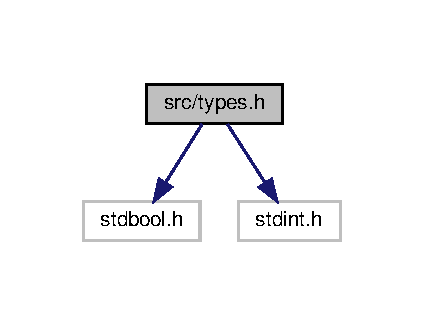
\includegraphics[width=204pt]{types_8h__incl}
\end{center}
\end{figure}
This graph shows which files directly or indirectly include this file\+:
\nopagebreak
\begin{figure}[H]
\begin{center}
\leavevmode
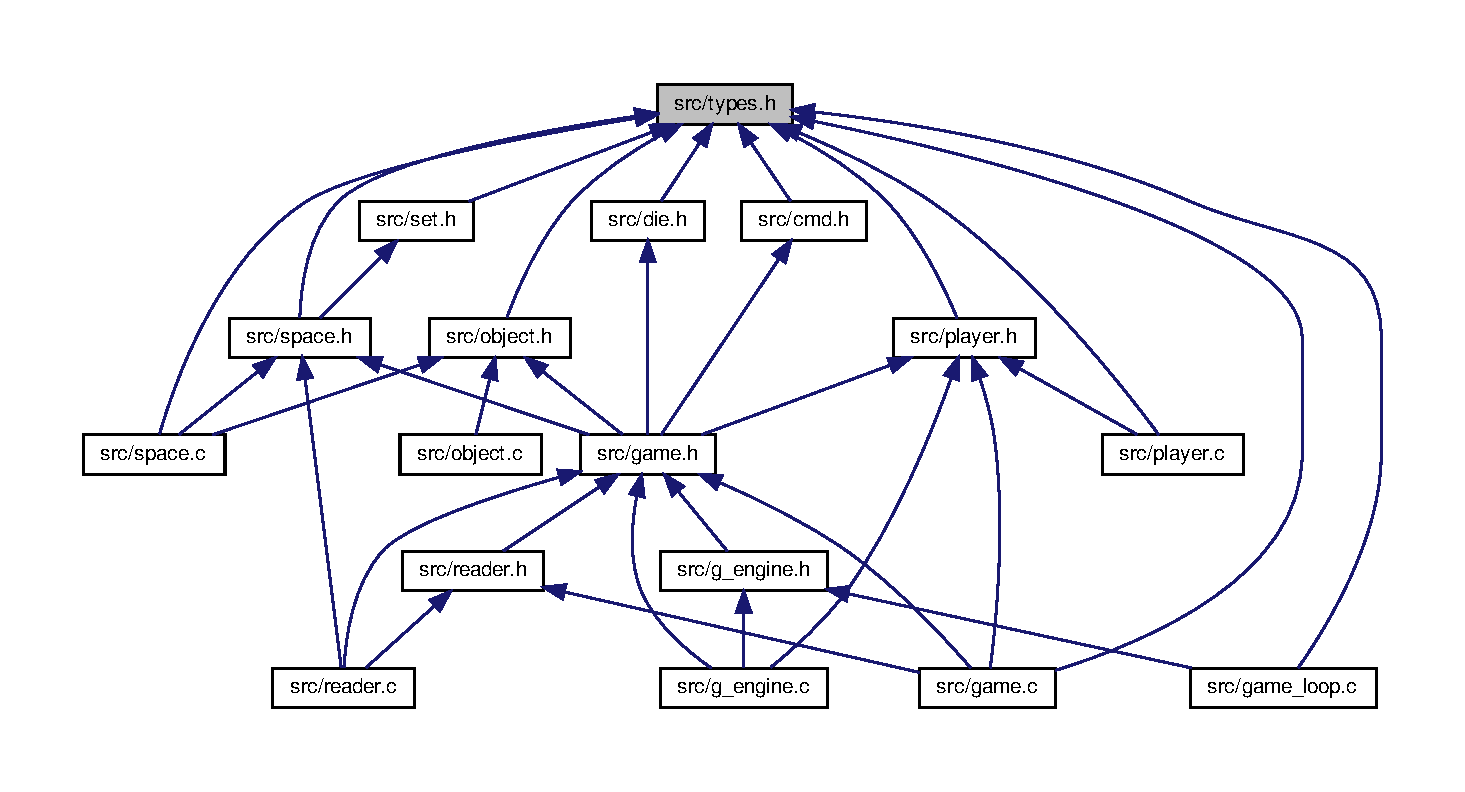
\includegraphics[width=350pt]{types_8h__dep__incl}
\end{center}
\end{figure}
\subsection*{Macros}
\begin{DoxyCompactItemize}
\item 
\mbox{\Hypertarget{types_8h_a92ed8507d1cd2331ad09275c5c4c1c89}\label{types_8h_a92ed8507d1cd2331ad09275c5c4c1c89}} 
\#define \hyperlink{types_8h_a92ed8507d1cd2331ad09275c5c4c1c89}{W\+O\+R\+D\+\_\+\+S\+I\+ZE}~1000
\begin{DoxyCompactList}\small\item\em Default strings buffer length. \end{DoxyCompactList}\item 
\mbox{\Hypertarget{types_8h_a642e16f35aa1e585c25e405ede76e115}\label{types_8h_a642e16f35aa1e585c25e405ede76e115}} 
\#define \hyperlink{types_8h_a642e16f35aa1e585c25e405ede76e115}{N\+O\+\_\+\+ID}~-\/1
\begin{DoxyCompactList}\small\item\em Value of N\+O\+\_\+\+ID. \end{DoxyCompactList}\end{DoxyCompactItemize}
\subsection*{Typedefs}
\begin{DoxyCompactItemize}
\item 
\mbox{\Hypertarget{types_8h_a845e604fb28f7e3d97549da3448149d3}\label{types_8h_a845e604fb28f7e3d97549da3448149d3}} 
typedef long \hyperlink{types_8h_a845e604fb28f7e3d97549da3448149d3}{Id}
\begin{DoxyCompactList}\small\item\em Defines an id as long. \end{DoxyCompactList}\end{DoxyCompactItemize}
\subsection*{Enumerations}
\begin{DoxyCompactItemize}
\item 
enum \hyperlink{types_8h_a32c27cc471df37f4fc818d65de0a56c4}{S\+T\+A\+T\+US} \{ \hyperlink{types_8h_a32c27cc471df37f4fc818d65de0a56c4a2fd6f336d08340583bd620a7f5694c90}{E\+R\+R\+OR}, 
\hyperlink{types_8h_a32c27cc471df37f4fc818d65de0a56c4a2bc49ec37d6a5715dd23e85f1ff5bb59}{OK}
 \}\begin{DoxyCompactList}\small\item\em Status variants. \end{DoxyCompactList}
\item 
enum \hyperlink{types_8h_a7a09f2d4d51c4b4ba7957bbe676a3855}{Cardinal\+Point} \{ \hyperlink{types_8h_a7a09f2d4d51c4b4ba7957bbe676a3855a2c63acbe79d9f41ba6bb7766e9c37702}{N}, 
\hyperlink{types_8h_a7a09f2d4d51c4b4ba7957bbe676a3855af1ce01387d2348f8b858721a7db81670}{S}, 
\hyperlink{types_8h_a7a09f2d4d51c4b4ba7957bbe676a3855ab199e021998d49b1f09338d8b9b18ecb}{E}, 
\hyperlink{types_8h_a7a09f2d4d51c4b4ba7957bbe676a3855ab722ceeb601c72cd78fbd35f3581fdf7}{W}
 \}\begin{DoxyCompactList}\small\item\em Direction\textquotesingle{}s structure. \end{DoxyCompactList}
\end{DoxyCompactItemize}


\subsection{Detailed Description}
It defines types of data. 

\begin{DoxyAuthor}{Author}
Miguel Rodríguez 
\end{DoxyAuthor}
\begin{DoxyVersion}{Version}
0.\+8.\+4 
\end{DoxyVersion}
\begin{DoxyDate}{Date}
18/03/2019 
\end{DoxyDate}


\subsection{Enumeration Type Documentation}
\mbox{\Hypertarget{types_8h_a32c27cc471df37f4fc818d65de0a56c4}\label{types_8h_a32c27cc471df37f4fc818d65de0a56c4}} 
\index{types.\+h@{types.\+h}!S\+T\+A\+T\+US@{S\+T\+A\+T\+US}}
\index{S\+T\+A\+T\+US@{S\+T\+A\+T\+US}!types.\+h@{types.\+h}}
\subsubsection{\texorpdfstring{S\+T\+A\+T\+US}{STATUS}}
{\footnotesize\ttfamily enum \hyperlink{types_8h_a32c27cc471df37f4fc818d65de0a56c4}{S\+T\+A\+T\+US}}



Status variants. 

\begin{DoxyEnumFields}{Enumerator}
\raisebox{\heightof{T}}[0pt][0pt]{\index{E\+R\+R\+OR@{E\+R\+R\+OR}!types.\+h@{types.\+h}}\index{types.\+h@{types.\+h}!E\+R\+R\+OR@{E\+R\+R\+OR}}}\mbox{\Hypertarget{types_8h_a32c27cc471df37f4fc818d65de0a56c4a2fd6f336d08340583bd620a7f5694c90}\label{types_8h_a32c27cc471df37f4fc818d65de0a56c4a2fd6f336d08340583bd620a7f5694c90}} 
E\+R\+R\+OR&Error means a failure. \\
\hline

\raisebox{\heightof{T}}[0pt][0pt]{\index{OK@{OK}!types.\+h@{types.\+h}}\index{types.\+h@{types.\+h}!OK@{OK}}}\mbox{\Hypertarget{types_8h_a32c27cc471df37f4fc818d65de0a56c4a2bc49ec37d6a5715dd23e85f1ff5bb59}\label{types_8h_a32c27cc471df37f4fc818d65de0a56c4a2bc49ec37d6a5715dd23e85f1ff5bb59}} 
OK&Ok means success. \\
\hline

\end{DoxyEnumFields}
\mbox{\Hypertarget{types_8h_a7a09f2d4d51c4b4ba7957bbe676a3855}\label{types_8h_a7a09f2d4d51c4b4ba7957bbe676a3855}} 
\index{types.\+h@{types.\+h}!Cardinal\+Point@{Cardinal\+Point}}
\index{Cardinal\+Point@{Cardinal\+Point}!types.\+h@{types.\+h}}
\subsubsection{\texorpdfstring{Cardinal\+Point}{CardinalPoint}}
{\footnotesize\ttfamily enum \hyperlink{types_8h_a7a09f2d4d51c4b4ba7957bbe676a3855}{Cardinal\+Point}}



Direction\textquotesingle{}s structure. 

\begin{DoxyEnumFields}{Enumerator}
\raisebox{\heightof{T}}[0pt][0pt]{\index{N@{N}!types.\+h@{types.\+h}}\index{types.\+h@{types.\+h}!N@{N}}}\mbox{\Hypertarget{types_8h_a7a09f2d4d51c4b4ba7957bbe676a3855a2c63acbe79d9f41ba6bb7766e9c37702}\label{types_8h_a7a09f2d4d51c4b4ba7957bbe676a3855a2c63acbe79d9f41ba6bb7766e9c37702}} 
N&North. \\
\hline

\raisebox{\heightof{T}}[0pt][0pt]{\index{S@{S}!types.\+h@{types.\+h}}\index{types.\+h@{types.\+h}!S@{S}}}\mbox{\Hypertarget{types_8h_a7a09f2d4d51c4b4ba7957bbe676a3855af1ce01387d2348f8b858721a7db81670}\label{types_8h_a7a09f2d4d51c4b4ba7957bbe676a3855af1ce01387d2348f8b858721a7db81670}} 
S&South. \\
\hline

\raisebox{\heightof{T}}[0pt][0pt]{\index{E@{E}!types.\+h@{types.\+h}}\index{types.\+h@{types.\+h}!E@{E}}}\mbox{\Hypertarget{types_8h_a7a09f2d4d51c4b4ba7957bbe676a3855ab199e021998d49b1f09338d8b9b18ecb}\label{types_8h_a7a09f2d4d51c4b4ba7957bbe676a3855ab199e021998d49b1f09338d8b9b18ecb}} 
E&East. \\
\hline

\raisebox{\heightof{T}}[0pt][0pt]{\index{W@{W}!types.\+h@{types.\+h}}\index{types.\+h@{types.\+h}!W@{W}}}\mbox{\Hypertarget{types_8h_a7a09f2d4d51c4b4ba7957bbe676a3855ab722ceeb601c72cd78fbd35f3581fdf7}\label{types_8h_a7a09f2d4d51c4b4ba7957bbe676a3855ab722ceeb601c72cd78fbd35f3581fdf7}} 
W&West. \\
\hline

\end{DoxyEnumFields}

\hypertarget{ui_8h}{}\section{src/ui.h File Reference}
\label{ui_8h}\index{src/ui.\+h@{src/ui.\+h}}


User interface based on chars.  


This graph shows which files directly or indirectly include this file\+:\nopagebreak
\begin{figure}[H]
\begin{center}
\leavevmode
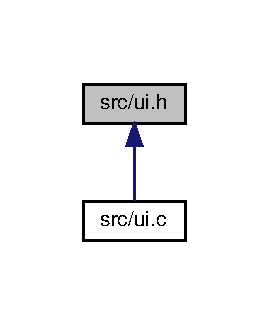
\includegraphics[width=160pt]{ui_8h__dep__incl}
\end{center}
\end{figure}
\subsection*{Macros}
\begin{DoxyCompactItemize}
\item 
\#define \hyperlink{ui_8h_abe040ae255b70ffb201aacc407ed614d}{M\+A\+X\+\_\+\+B\+O\+X\+ES}~10
\end{DoxyCompactItemize}
\subsection*{Typedefs}
\begin{DoxyCompactItemize}
\item 
\mbox{\Hypertarget{ui_8h_a5a605d1a8c0e2cfde565a0946fc3c3c8}\label{ui_8h_a5a605d1a8c0e2cfde565a0946fc3c3c8}} 
typedef struct \hyperlink{struct__Ui__screen}{\+\_\+\+Ui\+\_\+screen} {\bfseries Ui\+\_\+screen}
\item 
\mbox{\Hypertarget{ui_8h_a6faad303fab33e8efef93c4b8c0cf79a}\label{ui_8h_a6faad303fab33e8efef93c4b8c0cf79a}} 
typedef struct \hyperlink{struct__Ui__pix}{\+\_\+\+Ui\+\_\+pix} {\bfseries Ui\+\_\+pix}
\item 
\mbox{\Hypertarget{ui_8h_a9645c44adc241d19b9a6e555981a3d17}\label{ui_8h_a9645c44adc241d19b9a6e555981a3d17}} 
typedef struct \hyperlink{struct__Ui__box}{\+\_\+\+Ui\+\_\+box} {\bfseries Ui\+\_\+box}
\item 
\mbox{\Hypertarget{ui_8h_ad5baa06c5f7f2f943ddd440806930853}\label{ui_8h_ad5baa06c5f7f2f943ddd440806930853}} 
typedef struct \hyperlink{struct__Ui}{\+\_\+\+Ui} {\bfseries Ui}
\end{DoxyCompactItemize}
\subsection*{Enumerations}
\begin{DoxyCompactItemize}
\item 
\mbox{\Hypertarget{ui_8h_ab87bacfdad76e61b9412d7124be44c1c}\label{ui_8h_ab87bacfdad76e61b9412d7124be44c1c}} 
enum \hyperlink{ui_8h_ab87bacfdad76e61b9412d7124be44c1c}{Color} \{ \newline
{\bfseries B\+G\+\_\+\+B\+L\+A\+CK} =40, 
{\bfseries B\+G\+\_\+\+R\+ED} =41, 
{\bfseries B\+G\+\_\+\+G\+R\+E\+EN} =42, 
{\bfseries B\+G\+\_\+\+Y\+E\+L\+L\+OW} =43, 
\newline
{\bfseries B\+G\+\_\+\+B\+L\+UE} =44, 
{\bfseries B\+G\+\_\+\+P\+U\+R\+P\+LE} =45, 
{\bfseries B\+G\+\_\+\+C\+Y\+AN} =46, 
{\bfseries B\+G\+\_\+\+W\+H\+I\+TE} =47, 
\newline
{\bfseries F\+G\+\_\+\+B\+L\+A\+CK} =30, 
{\bfseries F\+G\+\_\+\+R\+ED} =31, 
{\bfseries F\+G\+\_\+\+G\+R\+E\+EN} =32, 
{\bfseries F\+G\+\_\+\+Y\+E\+L\+L\+OW} =33, 
\newline
{\bfseries F\+G\+\_\+\+B\+L\+UE} =34, 
{\bfseries F\+G\+\_\+\+P\+U\+R\+P\+LE} =35, 
{\bfseries F\+G\+\_\+\+C\+Y\+AN} =36, 
{\bfseries F\+G\+\_\+\+W\+H\+I\+TE} =37
 \}\begin{DoxyCompactList}\small\item\em Text formats. \end{DoxyCompactList}
\item 
enum \hyperlink{ui_8h_ab4e88c89b3b7ea1735996cc4def22d58}{Format} \{ \newline
\hyperlink{ui_8h_ab4e88c89b3b7ea1735996cc4def22d58a7ec4e09925986b754439a1f94a0d96db}{S\+\_\+\+D\+E\+F\+A\+U\+LT} =0, 
\hyperlink{ui_8h_ab4e88c89b3b7ea1735996cc4def22d58a102ce3bf8f47f2b8b10d2e3f872d8885}{S\+\_\+\+B\+O\+LD} =1, 
\hyperlink{ui_8h_ab4e88c89b3b7ea1735996cc4def22d58a853c3cc3fbd75aa00e16505d1242e575}{S\+\_\+\+D\+IM} =2, 
\hyperlink{ui_8h_ab4e88c89b3b7ea1735996cc4def22d58aae501dc5817876361aa06f3da39d1cfb}{S\+\_\+\+U\+N\+D\+E\+R\+L\+I\+N\+ED} =4, 
\newline
\hyperlink{ui_8h_ab4e88c89b3b7ea1735996cc4def22d58aa71a2dfb347a18e3a158667c17440ff2}{S\+\_\+\+B\+L\+I\+NK} =5, 
\hyperlink{ui_8h_ab4e88c89b3b7ea1735996cc4def22d58a12119c5fb581b9b351983dce8e0bf23d}{S\+\_\+\+R\+E\+V\+E\+R\+SE} =7, 
\hyperlink{ui_8h_ab4e88c89b3b7ea1735996cc4def22d58a2c4c9d9d754df0bfd7d1e82ba21acb40}{S\+\_\+\+H\+I\+D\+D\+EN} =9
 \}\begin{DoxyCompactList}\small\item\em Text formats. \end{DoxyCompactList}
\end{DoxyCompactItemize}
\subsection*{Functions}
\begin{DoxyCompactItemize}
\item 
\hyperlink{struct__Ui}{Ui} $\ast$ \hyperlink{ui_8h_adc8d261a6cf4862dc48958d7fdb5b9c6}{ui\+\_\+init} (int w, int h)
\item 
void \hyperlink{ui_8h_a26dcc63df2a1df20c72a9f8c9eb460d1}{ui\+\_\+destroy} (\hyperlink{struct__Ui}{Ui} $\ast$ui)
\item 
void \hyperlink{ui_8h_a02dd6678b83f5554e3614e455666b245}{ui\+\_\+draw} (\hyperlink{struct__Ui}{Ui} $\ast$ui)
\item 
void \hyperlink{ui_8h_af9b58458649ecd779d095f3d102d85c8}{ui\+\_\+clear} (\hyperlink{struct__Ui}{Ui} $\ast$ui)
\item 
void \hyperlink{ui_8h_a8e6b5fdd9c0dfd19c145a701b445ad05}{ui\+\_\+bg} (\hyperlink{struct__Ui}{Ui} $\ast$ui, \hyperlink{ui_8h_ab87bacfdad76e61b9412d7124be44c1c}{Color} c)
\item 
void \hyperlink{ui_8h_a70ca5594ea91504bec5a8a16826f3c23}{ui\+\_\+frm} (\hyperlink{struct__Ui}{Ui} $\ast$ui, int n,...)
\item 
void \hyperlink{ui_8h_ae33678d6064b4939cd98b2ba7b80357e}{ui\+\_\+rs} (\hyperlink{struct__Ui}{Ui} $\ast$ui)
\item 
void \hyperlink{ui_8h_a6eaad07fdf59b0544ee82c2ef461e0b1}{ui\+\_\+new\+\_\+box} (\hyperlink{struct__Ui}{Ui} $\ast$ui, int id, int x, int y, int w, int h)
\item 
void \hyperlink{ui_8h_aa1ded7a0cb2d451204058c0dfa70c27f}{ui\+\_\+box\+\_\+bg} (\hyperlink{struct__Ui}{Ui} $\ast$ui, int id, \hyperlink{ui_8h_ab87bacfdad76e61b9412d7124be44c1c}{Color} c)
\item 
void \hyperlink{ui_8h_a603e6d6365ab52e1ee44d11745d3267a}{ui\+\_\+box\+\_\+seek} (\hyperlink{struct__Ui}{Ui} $\ast$ui, int id, int x, int y)
\item 
void \hyperlink{ui_8h_a5f90f8ec38b654d40d68bf3b23542d20}{ui\+\_\+clear\+\_\+box} (\hyperlink{struct__Ui}{Ui} $\ast$ui, int id)
\item 
void \hyperlink{ui_8h_ab6a43ed5c9793ef4fc7f1c4ca35a8519}{ui\+\_\+box\+\_\+pad} (\hyperlink{struct__Ui}{Ui} $\ast$ui, int id, const char $\ast$pad)
\item 
void \hyperlink{ui_8h_a104d255f566d4579b63439f4dd06e802}{ui\+\_\+box\+\_\+put} (\hyperlink{struct__Ui}{Ui} $\ast$ui, int id, const char $\ast$str,...)
\end{DoxyCompactItemize}


\subsection{Detailed Description}
User interface based on chars. 

\begin{DoxyAuthor}{Author}
Javier Romera 
\end{DoxyAuthor}
\begin{DoxyVersion}{Version}
0.\+6.\+1 
\end{DoxyVersion}
\begin{DoxyDate}{Date}
17/03/2019 
\end{DoxyDate}
\begin{DoxyCopyright}{Copyright}
G\+NU Public License 
\end{DoxyCopyright}


\subsection{Macro Definition Documentation}
\mbox{\Hypertarget{ui_8h_abe040ae255b70ffb201aacc407ed614d}\label{ui_8h_abe040ae255b70ffb201aacc407ed614d}} 
\index{ui.\+h@{ui.\+h}!M\+A\+X\+\_\+\+B\+O\+X\+ES@{M\+A\+X\+\_\+\+B\+O\+X\+ES}}
\index{M\+A\+X\+\_\+\+B\+O\+X\+ES@{M\+A\+X\+\_\+\+B\+O\+X\+ES}!ui.\+h@{ui.\+h}}
\subsubsection{\texorpdfstring{M\+A\+X\+\_\+\+B\+O\+X\+ES}{MAX\_BOXES}}
{\footnotesize\ttfamily \#define M\+A\+X\+\_\+\+B\+O\+X\+ES~10}

Maximum number of boxes 

\subsection{Enumeration Type Documentation}
\mbox{\Hypertarget{ui_8h_ab4e88c89b3b7ea1735996cc4def22d58}\label{ui_8h_ab4e88c89b3b7ea1735996cc4def22d58}} 
\index{ui.\+h@{ui.\+h}!Format@{Format}}
\index{Format@{Format}!ui.\+h@{ui.\+h}}
\subsubsection{\texorpdfstring{Format}{Format}}
{\footnotesize\ttfamily enum \hyperlink{ui_8h_ab4e88c89b3b7ea1735996cc4def22d58}{Format}}



Text formats. 

\begin{DoxyEnumFields}{Enumerator}
\raisebox{\heightof{T}}[0pt][0pt]{\index{S\+\_\+\+D\+E\+F\+A\+U\+LT@{S\+\_\+\+D\+E\+F\+A\+U\+LT}!ui.\+h@{ui.\+h}}\index{ui.\+h@{ui.\+h}!S\+\_\+\+D\+E\+F\+A\+U\+LT@{S\+\_\+\+D\+E\+F\+A\+U\+LT}}}\mbox{\Hypertarget{ui_8h_ab4e88c89b3b7ea1735996cc4def22d58a7ec4e09925986b754439a1f94a0d96db}\label{ui_8h_ab4e88c89b3b7ea1735996cc4def22d58a7ec4e09925986b754439a1f94a0d96db}} 
S\+\_\+\+D\+E\+F\+A\+U\+LT&Resets text format \\
\hline

\raisebox{\heightof{T}}[0pt][0pt]{\index{S\+\_\+\+B\+O\+LD@{S\+\_\+\+B\+O\+LD}!ui.\+h@{ui.\+h}}\index{ui.\+h@{ui.\+h}!S\+\_\+\+B\+O\+LD@{S\+\_\+\+B\+O\+LD}}}\mbox{\Hypertarget{ui_8h_ab4e88c89b3b7ea1735996cc4def22d58a102ce3bf8f47f2b8b10d2e3f872d8885}\label{ui_8h_ab4e88c89b3b7ea1735996cc4def22d58a102ce3bf8f47f2b8b10d2e3f872d8885}} 
S\+\_\+\+B\+O\+LD&Bold text \\
\hline

\raisebox{\heightof{T}}[0pt][0pt]{\index{S\+\_\+\+D\+IM@{S\+\_\+\+D\+IM}!ui.\+h@{ui.\+h}}\index{ui.\+h@{ui.\+h}!S\+\_\+\+D\+IM@{S\+\_\+\+D\+IM}}}\mbox{\Hypertarget{ui_8h_ab4e88c89b3b7ea1735996cc4def22d58a853c3cc3fbd75aa00e16505d1242e575}\label{ui_8h_ab4e88c89b3b7ea1735996cc4def22d58a853c3cc3fbd75aa00e16505d1242e575}} 
S\+\_\+\+D\+IM&Small text \\
\hline

\raisebox{\heightof{T}}[0pt][0pt]{\index{S\+\_\+\+U\+N\+D\+E\+R\+L\+I\+N\+ED@{S\+\_\+\+U\+N\+D\+E\+R\+L\+I\+N\+ED}!ui.\+h@{ui.\+h}}\index{ui.\+h@{ui.\+h}!S\+\_\+\+U\+N\+D\+E\+R\+L\+I\+N\+ED@{S\+\_\+\+U\+N\+D\+E\+R\+L\+I\+N\+ED}}}\mbox{\Hypertarget{ui_8h_ab4e88c89b3b7ea1735996cc4def22d58aae501dc5817876361aa06f3da39d1cfb}\label{ui_8h_ab4e88c89b3b7ea1735996cc4def22d58aae501dc5817876361aa06f3da39d1cfb}} 
S\+\_\+\+U\+N\+D\+E\+R\+L\+I\+N\+ED&Underlined text \\
\hline

\raisebox{\heightof{T}}[0pt][0pt]{\index{S\+\_\+\+B\+L\+I\+NK@{S\+\_\+\+B\+L\+I\+NK}!ui.\+h@{ui.\+h}}\index{ui.\+h@{ui.\+h}!S\+\_\+\+B\+L\+I\+NK@{S\+\_\+\+B\+L\+I\+NK}}}\mbox{\Hypertarget{ui_8h_ab4e88c89b3b7ea1735996cc4def22d58aa71a2dfb347a18e3a158667c17440ff2}\label{ui_8h_ab4e88c89b3b7ea1735996cc4def22d58aa71a2dfb347a18e3a158667c17440ff2}} 
S\+\_\+\+B\+L\+I\+NK&Blink text \\
\hline

\raisebox{\heightof{T}}[0pt][0pt]{\index{S\+\_\+\+R\+E\+V\+E\+R\+SE@{S\+\_\+\+R\+E\+V\+E\+R\+SE}!ui.\+h@{ui.\+h}}\index{ui.\+h@{ui.\+h}!S\+\_\+\+R\+E\+V\+E\+R\+SE@{S\+\_\+\+R\+E\+V\+E\+R\+SE}}}\mbox{\Hypertarget{ui_8h_ab4e88c89b3b7ea1735996cc4def22d58a12119c5fb581b9b351983dce8e0bf23d}\label{ui_8h_ab4e88c89b3b7ea1735996cc4def22d58a12119c5fb581b9b351983dce8e0bf23d}} 
S\+\_\+\+R\+E\+V\+E\+R\+SE&Reversed text format \\
\hline

\raisebox{\heightof{T}}[0pt][0pt]{\index{S\+\_\+\+H\+I\+D\+D\+EN@{S\+\_\+\+H\+I\+D\+D\+EN}!ui.\+h@{ui.\+h}}\index{ui.\+h@{ui.\+h}!S\+\_\+\+H\+I\+D\+D\+EN@{S\+\_\+\+H\+I\+D\+D\+EN}}}\mbox{\Hypertarget{ui_8h_ab4e88c89b3b7ea1735996cc4def22d58a2c4c9d9d754df0bfd7d1e82ba21acb40}\label{ui_8h_ab4e88c89b3b7ea1735996cc4def22d58a2c4c9d9d754df0bfd7d1e82ba21acb40}} 
S\+\_\+\+H\+I\+D\+D\+EN&Hidden text \\
\hline

\end{DoxyEnumFields}


\subsection{Function Documentation}
\mbox{\Hypertarget{ui_8h_adc8d261a6cf4862dc48958d7fdb5b9c6}\label{ui_8h_adc8d261a6cf4862dc48958d7fdb5b9c6}} 
\index{ui.\+h@{ui.\+h}!ui\+\_\+init@{ui\+\_\+init}}
\index{ui\+\_\+init@{ui\+\_\+init}!ui.\+h@{ui.\+h}}
\subsubsection{\texorpdfstring{ui\+\_\+init()}{ui\_init()}}
{\footnotesize\ttfamily \hyperlink{struct__Ui}{Ui}$\ast$ ui\+\_\+init (\begin{DoxyParamCaption}\item[{int}]{w,  }\item[{int}]{h }\end{DoxyParamCaption})}

Initializes UI struct 
\begin{DoxyParams}{Parameters}
{\em \{int\}} & w -\/ The width of the user interface based on chars \\
\hline
{\em \{int\}} & h -\/ The height of the user interface based on chars \\
\hline
\end{DoxyParams}

\begin{DoxyRetVals}{Return values}
{\em \{\+Ui$\ast$\}} & -\/ Returns an UI pointer \\
\hline
\end{DoxyRetVals}
\mbox{\Hypertarget{ui_8h_a26dcc63df2a1df20c72a9f8c9eb460d1}\label{ui_8h_a26dcc63df2a1df20c72a9f8c9eb460d1}} 
\index{ui.\+h@{ui.\+h}!ui\+\_\+destroy@{ui\+\_\+destroy}}
\index{ui\+\_\+destroy@{ui\+\_\+destroy}!ui.\+h@{ui.\+h}}
\subsubsection{\texorpdfstring{ui\+\_\+destroy()}{ui\_destroy()}}
{\footnotesize\ttfamily void ui\+\_\+destroy (\begin{DoxyParamCaption}\item[{\hyperlink{struct__Ui}{Ui} $\ast$}]{ui }\end{DoxyParamCaption})}

Destroys UI struct 
\begin{DoxyParams}{Parameters}
{\em \{\+Ui$\ast$\}} & ui -\/ A pointer to the UI struct \\
\hline
\end{DoxyParams}
\mbox{\Hypertarget{ui_8h_a02dd6678b83f5554e3614e455666b245}\label{ui_8h_a02dd6678b83f5554e3614e455666b245}} 
\index{ui.\+h@{ui.\+h}!ui\+\_\+draw@{ui\+\_\+draw}}
\index{ui\+\_\+draw@{ui\+\_\+draw}!ui.\+h@{ui.\+h}}
\subsubsection{\texorpdfstring{ui\+\_\+draw()}{ui\_draw()}}
{\footnotesize\ttfamily void ui\+\_\+draw (\begin{DoxyParamCaption}\item[{\hyperlink{struct__Ui}{Ui} $\ast$}]{ui }\end{DoxyParamCaption})}

Prints all buffered data inside the UI into the stdout 
\begin{DoxyParams}{Parameters}
{\em \{\+Ui$\ast$\}} & ui -\/ The UI that sueld be printed \\
\hline
\end{DoxyParams}
\mbox{\Hypertarget{ui_8h_af9b58458649ecd779d095f3d102d85c8}\label{ui_8h_af9b58458649ecd779d095f3d102d85c8}} 
\index{ui.\+h@{ui.\+h}!ui\+\_\+clear@{ui\+\_\+clear}}
\index{ui\+\_\+clear@{ui\+\_\+clear}!ui.\+h@{ui.\+h}}
\subsubsection{\texorpdfstring{ui\+\_\+clear()}{ui\_clear()}}
{\footnotesize\ttfamily void ui\+\_\+clear (\begin{DoxyParamCaption}\item[{\hyperlink{struct__Ui}{Ui} $\ast$}]{ui }\end{DoxyParamCaption})}

Clears all the UI data, including inherit objects like boxes, shapes, ... 
\begin{DoxyParams}{Parameters}
{\em \{\+Ui$\ast$\}} & ui -\/ The UI that should be clered \\
\hline
\end{DoxyParams}
\mbox{\Hypertarget{ui_8h_a8e6b5fdd9c0dfd19c145a701b445ad05}\label{ui_8h_a8e6b5fdd9c0dfd19c145a701b445ad05}} 
\index{ui.\+h@{ui.\+h}!ui\+\_\+bg@{ui\+\_\+bg}}
\index{ui\+\_\+bg@{ui\+\_\+bg}!ui.\+h@{ui.\+h}}
\subsubsection{\texorpdfstring{ui\+\_\+bg()}{ui\_bg()}}
{\footnotesize\ttfamily void ui\+\_\+bg (\begin{DoxyParamCaption}\item[{\hyperlink{struct__Ui}{Ui} $\ast$}]{ui,  }\item[{\hyperlink{ui_8h_ab87bacfdad76e61b9412d7124be44c1c}{Color}}]{c }\end{DoxyParamCaption})}

Fills the main UI background with a given color 
\begin{DoxyParams}{Parameters}
{\em \{\+Ui$\ast$\}} & ui -\/ UI to be filled \\
\hline
{\em \{\+Color\}} & c -\/ The color with which the background will be filled \\
\hline
\end{DoxyParams}
\mbox{\Hypertarget{ui_8h_a70ca5594ea91504bec5a8a16826f3c23}\label{ui_8h_a70ca5594ea91504bec5a8a16826f3c23}} 
\index{ui.\+h@{ui.\+h}!ui\+\_\+frm@{ui\+\_\+frm}}
\index{ui\+\_\+frm@{ui\+\_\+frm}!ui.\+h@{ui.\+h}}
\subsubsection{\texorpdfstring{ui\+\_\+frm()}{ui\_frm()}}
{\footnotesize\ttfamily void ui\+\_\+frm (\begin{DoxyParamCaption}\item[{\hyperlink{struct__Ui}{Ui} $\ast$}]{ui,  }\item[{int}]{n,  }\item[{}]{... }\end{DoxyParamCaption})}

Sets a temporary format of the UI This means that all the text, shapes and other items will use the format that was setted in the last \hyperlink{ui_8h_a70ca5594ea91504bec5a8a16826f3c23}{ui\+\_\+frm()} call 
\begin{DoxyParams}{Parameters}
{\em \{\+Ui$\ast$\}} & ui -\/ UI to set the temporary parameters \\
\hline
{\em \{int\}} & n -\/ The number of parameters that will be set \\
\hline
{\em \{int\}} & ... -\/ The N parameters to be set, like B\+G\+\_\+\+R\+ED, S\+\_\+\+B\+O\+LD, ... \\
\hline
\end{DoxyParams}
\mbox{\Hypertarget{ui_8h_ae33678d6064b4939cd98b2ba7b80357e}\label{ui_8h_ae33678d6064b4939cd98b2ba7b80357e}} 
\index{ui.\+h@{ui.\+h}!ui\+\_\+rs@{ui\+\_\+rs}}
\index{ui\+\_\+rs@{ui\+\_\+rs}!ui.\+h@{ui.\+h}}
\subsubsection{\texorpdfstring{ui\+\_\+rs()}{ui\_rs()}}
{\footnotesize\ttfamily void ui\+\_\+rs (\begin{DoxyParamCaption}\item[{\hyperlink{struct__Ui}{Ui} $\ast$}]{ui }\end{DoxyParamCaption})}

Resets the temporary format of the UI to default 
\begin{DoxyParams}{Parameters}
{\em \{\+Ui$\ast$\}} & ui -\/ the UI where the temporary parameters should be resetted \\
\hline
\end{DoxyParams}
\mbox{\Hypertarget{ui_8h_a6eaad07fdf59b0544ee82c2ef461e0b1}\label{ui_8h_a6eaad07fdf59b0544ee82c2ef461e0b1}} 
\index{ui.\+h@{ui.\+h}!ui\+\_\+new\+\_\+box@{ui\+\_\+new\+\_\+box}}
\index{ui\+\_\+new\+\_\+box@{ui\+\_\+new\+\_\+box}!ui.\+h@{ui.\+h}}
\subsubsection{\texorpdfstring{ui\+\_\+new\+\_\+box()}{ui\_new\_box()}}
{\footnotesize\ttfamily void ui\+\_\+new\+\_\+box (\begin{DoxyParamCaption}\item[{\hyperlink{struct__Ui}{Ui} $\ast$}]{ui,  }\item[{int}]{id,  }\item[{int}]{x,  }\item[{int}]{y,  }\item[{int}]{w,  }\item[{int}]{h }\end{DoxyParamCaption})}

Creates a new box 
\begin{DoxyParams}{Parameters}
{\em \{\+Ui$\ast$\}} & ui -\/ UI where the box should be used \\
\hline
{\em \{int\}} & id -\/ The ID with which the box will be referenced \\
\hline
{\em \{int\}} & x -\/ The x position of the box ( col of the matrix ) \\
\hline
{\em \{int\}} & y -\/ The y position of the box ( row of the matrix ) \\
\hline
{\em \{int\}} & w -\/ The width of the box ( number of cols ) \\
\hline
{\em \{int\}} & h -\/ The height of the box ( number of rows ) \\
\hline
\end{DoxyParams}
\mbox{\Hypertarget{ui_8h_aa1ded7a0cb2d451204058c0dfa70c27f}\label{ui_8h_aa1ded7a0cb2d451204058c0dfa70c27f}} 
\index{ui.\+h@{ui.\+h}!ui\+\_\+box\+\_\+bg@{ui\+\_\+box\+\_\+bg}}
\index{ui\+\_\+box\+\_\+bg@{ui\+\_\+box\+\_\+bg}!ui.\+h@{ui.\+h}}
\subsubsection{\texorpdfstring{ui\+\_\+box\+\_\+bg()}{ui\_box\_bg()}}
{\footnotesize\ttfamily void ui\+\_\+box\+\_\+bg (\begin{DoxyParamCaption}\item[{\hyperlink{struct__Ui}{Ui} $\ast$}]{ui,  }\item[{int}]{id,  }\item[{\hyperlink{ui_8h_ab87bacfdad76e61b9412d7124be44c1c}{Color}}]{c }\end{DoxyParamCaption})}

Fills the main box background with a given color This function does N\+OT clear the box buffer 
\begin{DoxyParams}{Parameters}
{\em \{\+Ui$\ast$\}} & ui -\/ UI where the box is located \\
\hline
{\em \{int\}} & id -\/ The id of the box \\
\hline
{\em \{\+Color\}} & c -\/ The color with which the background will be filled \\
\hline
\end{DoxyParams}
\mbox{\Hypertarget{ui_8h_a603e6d6365ab52e1ee44d11745d3267a}\label{ui_8h_a603e6d6365ab52e1ee44d11745d3267a}} 
\index{ui.\+h@{ui.\+h}!ui\+\_\+box\+\_\+seek@{ui\+\_\+box\+\_\+seek}}
\index{ui\+\_\+box\+\_\+seek@{ui\+\_\+box\+\_\+seek}!ui.\+h@{ui.\+h}}
\subsubsection{\texorpdfstring{ui\+\_\+box\+\_\+seek()}{ui\_box\_seek()}}
{\footnotesize\ttfamily void ui\+\_\+box\+\_\+seek (\begin{DoxyParamCaption}\item[{\hyperlink{struct__Ui}{Ui} $\ast$}]{ui,  }\item[{int}]{id,  }\item[{int}]{x,  }\item[{int}]{y }\end{DoxyParamCaption})}

Changes the cursor position of a box 
\begin{DoxyParams}{Parameters}
{\em \{\+Ui$\ast$\}} & ui -\/ UI where the box is located \\
\hline
{\em \{int\}} & id -\/ The id of the box \\
\hline
{\em \{int\}} & x -\/ Cursor x position ( col matrix ) \\
\hline
{\em \{int\}} & y -\/ Curosr y position ( row matrix ) \\
\hline
\end{DoxyParams}
\mbox{\Hypertarget{ui_8h_a5f90f8ec38b654d40d68bf3b23542d20}\label{ui_8h_a5f90f8ec38b654d40d68bf3b23542d20}} 
\index{ui.\+h@{ui.\+h}!ui\+\_\+clear\+\_\+box@{ui\+\_\+clear\+\_\+box}}
\index{ui\+\_\+clear\+\_\+box@{ui\+\_\+clear\+\_\+box}!ui.\+h@{ui.\+h}}
\subsubsection{\texorpdfstring{ui\+\_\+clear\+\_\+box()}{ui\_clear\_box()}}
{\footnotesize\ttfamily void ui\+\_\+clear\+\_\+box (\begin{DoxyParamCaption}\item[{\hyperlink{struct__Ui}{Ui} $\ast$}]{ui,  }\item[{int}]{id }\end{DoxyParamCaption})}

Clears the box buffer 
\begin{DoxyParams}{Parameters}
{\em \{\+Ui$\ast$\}} & ui -\/ UI where the box is located \\
\hline
{\em \{int\}} & id -\/ The id of the box \\
\hline
\end{DoxyParams}
\mbox{\Hypertarget{ui_8h_ab6a43ed5c9793ef4fc7f1c4ca35a8519}\label{ui_8h_ab6a43ed5c9793ef4fc7f1c4ca35a8519}} 
\index{ui.\+h@{ui.\+h}!ui\+\_\+box\+\_\+pad@{ui\+\_\+box\+\_\+pad}}
\index{ui\+\_\+box\+\_\+pad@{ui\+\_\+box\+\_\+pad}!ui.\+h@{ui.\+h}}
\subsubsection{\texorpdfstring{ui\+\_\+box\+\_\+pad()}{ui\_box\_pad()}}
{\footnotesize\ttfamily void ui\+\_\+box\+\_\+pad (\begin{DoxyParamCaption}\item[{\hyperlink{struct__Ui}{Ui} $\ast$}]{ui,  }\item[{int}]{id,  }\item[{const char $\ast$}]{pad }\end{DoxyParamCaption})}

Sets the padding of a box 
\begin{DoxyParams}{Parameters}
{\em \{\+Ui$\ast$\}} & ui -\/ UI where the box is located \\
\hline
{\em \{int\}} & id -\/ The id of the box \\
\hline
{\em \{char$\ast$\}} & pad -\/ The padding of the box \char`\"{}$<$top$>$ $<$right$>$ $<$bottom$>$ $<$left$>$\char`\"{} \\
\hline
\end{DoxyParams}
\mbox{\Hypertarget{ui_8h_a104d255f566d4579b63439f4dd06e802}\label{ui_8h_a104d255f566d4579b63439f4dd06e802}} 
\index{ui.\+h@{ui.\+h}!ui\+\_\+box\+\_\+put@{ui\+\_\+box\+\_\+put}}
\index{ui\+\_\+box\+\_\+put@{ui\+\_\+box\+\_\+put}!ui.\+h@{ui.\+h}}
\subsubsection{\texorpdfstring{ui\+\_\+box\+\_\+put()}{ui\_box\_put()}}
{\footnotesize\ttfamily void ui\+\_\+box\+\_\+put (\begin{DoxyParamCaption}\item[{\hyperlink{struct__Ui}{Ui} $\ast$}]{ui,  }\item[{int}]{id,  }\item[{const char $\ast$}]{str,  }\item[{}]{... }\end{DoxyParamCaption})}

Updates the box buffer with a given string 
\begin{DoxyParams}{Parameters}
{\em \{\+Ui$\ast$\}} & ui -\/ UI where the box is located \\
\hline
{\em \{int\}} & id -\/ The id of the box \\
\hline
{\em \{char$\ast$\}} & str -\/ String format \\
\hline
{\em \{...\}} & -\/ String format arguments \\
\hline
\end{DoxyParams}

\hypertarget{cmd_8c}{}\section{src/cmd.c File Reference}
\label{cmd_8c}\index{src/cmd.\+c@{src/cmd.\+c}}


Command source code.  


{\ttfamily \#include \char`\"{}cmd.\+h\char`\"{}}\newline
{\ttfamily \#include $<$stdio.\+h$>$}\newline
{\ttfamily \#include $<$stdlib.\+h$>$}\newline
{\ttfamily \#include $<$string.\+h$>$}\newline
{\ttfamily \#include $<$stdarg.\+h$>$}\newline
{\ttfamily \#include $<$unistd.\+h$>$}\newline
Include dependency graph for cmd.\+c\+:\nopagebreak
\begin{figure}[H]
\begin{center}
\leavevmode
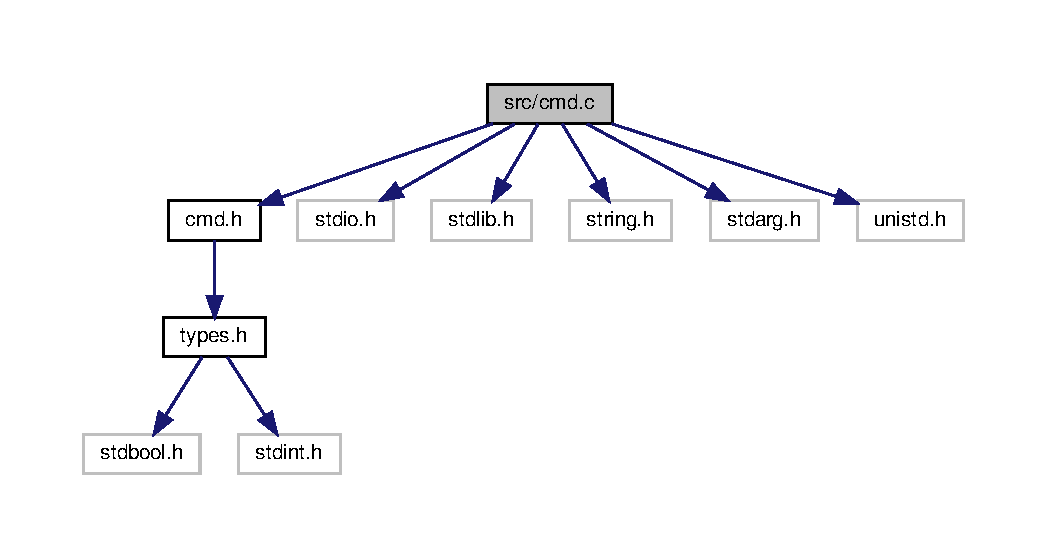
\includegraphics[width=350pt]{cmd_8c__incl}
\end{center}
\end{figure}
\subsection*{Data Structures}
\begin{DoxyCompactItemize}
\item 
struct \hyperlink{struct__Cmd}{\+\_\+\+Cmd}
\begin{DoxyCompactList}\small\item\em Command data structure. \end{DoxyCompactList}\end{DoxyCompactItemize}
\subsection*{Functions}
\begin{DoxyCompactItemize}
\item 
void \hyperlink{cmd_8c_a41754cc6e6c54b0caa4d19371cfa37da}{cmd\+\_\+argv\+\_\+free} (\hyperlink{cmd_8h_ab2b68b94b84c77ba11a699a76b8cf9cc}{Cmd} $\ast$cmd)
\begin{DoxyCompactList}\small\item\em Frees the argument values of a given command. \end{DoxyCompactList}\item 
void \hyperlink{cmd_8c_a90bbf69ef685a531b43ac4084c5fa571}{cmd\+\_\+build} (\hyperlink{cmd_8h_a2933336e1f8003400f3b050402f0f5f3}{Cid} id, const char $\ast$b\+\_\+name, const char $\ast$s\+\_\+name, \hyperlink{cmd_8h_a78d7a8bd781b5514e6dd7e1253bb1907}{cmd\+\_\+fn} fn)
\begin{DoxyCompactList}\small\item\em Sets up a new command and stores it inside a private array. \end{DoxyCompactList}\item 
\mbox{\Hypertarget{cmd_8c_a3078f0effe67b212b1b913e3ff0c08dc}\label{cmd_8c_a3078f0effe67b212b1b913e3ff0c08dc}} 
void \hyperlink{cmd_8c_a3078f0effe67b212b1b913e3ff0c08dc}{cmd\+\_\+free} ()
\begin{DoxyCompactList}\small\item\em Destroy all the setted commands. \end{DoxyCompactList}\item 
const char $\ast$ \hyperlink{cmd_8c_aa1e02137469ddc06fa9bcb3dac2c3a56}{cmd\+\_\+get\+\_\+argv} (\hyperlink{cmd_8h_ab2b68b94b84c77ba11a699a76b8cf9cc}{Cmd} $\ast$cmd, int idx)
\begin{DoxyCompactList}\small\item\em Gets the desired indexed argument. \end{DoxyCompactList}\item 
const char $\ast$ \hyperlink{cmd_8c_afc6f99e63609bd15653ea164fbe59ede}{cmd\+\_\+get\+\_\+bname} (\hyperlink{cmd_8h_ab2b68b94b84c77ba11a699a76b8cf9cc}{Cmd} $\ast$cmd)
\begin{DoxyCompactList}\small\item\em Gets the base name of a given command. \end{DoxyCompactList}\item 
const char $\ast$ \hyperlink{cmd_8c_aa3bd4090b15be64bd3d4839233f85ee9}{cmd\+\_\+get\+\_\+sname} (\hyperlink{cmd_8h_ab2b68b94b84c77ba11a699a76b8cf9cc}{Cmd} $\ast$cmd)
\begin{DoxyCompactList}\small\item\em Gets the short name of a given command. \end{DoxyCompactList}\item 
const \hyperlink{cmd_8h_a2933336e1f8003400f3b050402f0f5f3}{Cid} \hyperlink{cmd_8c_a399883b5394d12f2c19816e72a756245}{cmd\+\_\+get\+\_\+cid} (\hyperlink{cmd_8h_ab2b68b94b84c77ba11a699a76b8cf9cc}{Cmd} $\ast$cmd)
\begin{DoxyCompactList}\small\item\em Gets the command id. \end{DoxyCompactList}\item 
const int \hyperlink{cmd_8c_a45b6622fba552dd2b1c620afb4af451c}{cmd\+\_\+get\+\_\+argc} (\hyperlink{cmd_8h_ab2b68b94b84c77ba11a699a76b8cf9cc}{Cmd} $\ast$cmd)
\begin{DoxyCompactList}\small\item\em Gets the number of arguemnts of a given command. \end{DoxyCompactList}\item 
\mbox{\Hypertarget{cmd_8c_a3787fda022912652a1f98b9c6b8441d3}\label{cmd_8c_a3787fda022912652a1f98b9c6b8441d3}} 
void {\bfseries cmd\+\_\+set\+\_\+ans} (\hyperlink{cmd_8h_ab2b68b94b84c77ba11a699a76b8cf9cc}{Cmd} $\ast$cmd, int errc, const char $\ast$frm,...)
\item 
const int \hyperlink{cmd_8c_a57baf1963c86de1643043f9c4cee9567}{cmd\+\_\+get\+\_\+errc} (\hyperlink{cmd_8h_ab2b68b94b84c77ba11a699a76b8cf9cc}{Cmd} $\ast$cmd)
\begin{DoxyCompactList}\small\item\em Gets the error code of a given command. \end{DoxyCompactList}\item 
const char $\ast$ \hyperlink{cmd_8c_a9fc56f507a2e6dabe93d8e8e03a81164}{cmd\+\_\+get\+\_\+ans} (\hyperlink{cmd_8h_ab2b68b94b84c77ba11a699a76b8cf9cc}{Cmd} $\ast$cmd)
\begin{DoxyCompactList}\small\item\em Gets a previus answer of the given command. \end{DoxyCompactList}\item 
\hyperlink{cmd_8h_ab2b68b94b84c77ba11a699a76b8cf9cc}{Cmd} $\ast$ \hyperlink{cmd_8c_ad26761936b79469541883548b5a69e02}{cmd\+\_\+get\+\_\+by\+\_\+cid} (\hyperlink{cmd_8h_a2933336e1f8003400f3b050402f0f5f3}{Cid} id)
\begin{DoxyCompactList}\small\item\em Gets a command by its id. \end{DoxyCompactList}\item 
\hyperlink{cmd_8h_ab2b68b94b84c77ba11a699a76b8cf9cc}{Cmd} $\ast$ \hyperlink{cmd_8c_afce1f6a7a163afaac5ffe4ca55faee59}{cmd\+\_\+get\+\_\+by\+\_\+name} (const char $\ast$n)
\begin{DoxyCompactList}\small\item\em Gets a command by its id. \end{DoxyCompactList}\item 
void \hyperlink{cmd_8c_a5090e929f5e97aa5492b47dfd7a6ec91}{cmd\+\_\+cb} (\hyperlink{cmd_8h_ab2b68b94b84c77ba11a699a76b8cf9cc}{Cmd} $\ast$cmd, void $\ast$vp)
\begin{DoxyCompactList}\small\item\em Calls to the callback function stored in the given command. \end{DoxyCompactList}\item 
\hyperlink{cmd_8h_ab2b68b94b84c77ba11a699a76b8cf9cc}{Cmd} $\ast$ \hyperlink{cmd_8c_abb04779da8a594a45843a10b91e9e3a3}{cmd\+\_\+req} ()
\begin{DoxyCompactList}\small\item\em Requests a new command from stdin. \end{DoxyCompactList}\end{DoxyCompactItemize}
\subsection*{Variables}
\begin{DoxyCompactItemize}
\item 
\mbox{\Hypertarget{cmd_8c_a3660f29836df7f6e9098155b8dc20bb8}\label{cmd_8c_a3660f29836df7f6e9098155b8dc20bb8}} 
\hyperlink{cmd_8h_ab2b68b94b84c77ba11a699a76b8cf9cc}{Cmd} $\ast$ \hyperlink{cmd_8c_a3660f29836df7f6e9098155b8dc20bb8}{C\+M\+DS} \mbox{[}\hyperlink{cmd_8h_ad14effda14501a769b3d46984d43aa00}{M\+A\+X\+\_\+\+C\+M\+DS}\mbox{]}
\begin{DoxyCompactList}\small\item\em Array where known commands will be stored. \end{DoxyCompactList}\end{DoxyCompactItemize}


\subsection{Detailed Description}
Command source code. 

\begin{DoxyAuthor}{Author}
Javier Romera 
\end{DoxyAuthor}
\begin{DoxyVersion}{Version}
0.\+8.\+4 
\end{DoxyVersion}
\begin{DoxyDate}{Date}
17/03/2019 
\end{DoxyDate}
\begin{DoxyCopyright}{Copyright}
G\+NU Public License 
\end{DoxyCopyright}


\subsection{Function Documentation}
\mbox{\Hypertarget{cmd_8c_a41754cc6e6c54b0caa4d19371cfa37da}\label{cmd_8c_a41754cc6e6c54b0caa4d19371cfa37da}} 
\index{cmd.\+c@{cmd.\+c}!cmd\+\_\+argv\+\_\+free@{cmd\+\_\+argv\+\_\+free}}
\index{cmd\+\_\+argv\+\_\+free@{cmd\+\_\+argv\+\_\+free}!cmd.\+c@{cmd.\+c}}
\subsubsection{\texorpdfstring{cmd\+\_\+argv\+\_\+free()}{cmd\_argv\_free()}}
{\footnotesize\ttfamily void cmd\+\_\+argv\+\_\+free (\begin{DoxyParamCaption}\item[{\hyperlink{cmd_8h_ab2b68b94b84c77ba11a699a76b8cf9cc}{Cmd} $\ast$}]{cmd }\end{DoxyParamCaption})}



Frees the argument values of a given command. 


\begin{DoxyParams}{Parameters}
{\em \{\+Cmd$\ast$\}} & cmd -\/ Command to be manipulated \\
\hline
\end{DoxyParams}
\mbox{\Hypertarget{cmd_8c_a90bbf69ef685a531b43ac4084c5fa571}\label{cmd_8c_a90bbf69ef685a531b43ac4084c5fa571}} 
\index{cmd.\+c@{cmd.\+c}!cmd\+\_\+build@{cmd\+\_\+build}}
\index{cmd\+\_\+build@{cmd\+\_\+build}!cmd.\+c@{cmd.\+c}}
\subsubsection{\texorpdfstring{cmd\+\_\+build()}{cmd\_build()}}
{\footnotesize\ttfamily void cmd\+\_\+build (\begin{DoxyParamCaption}\item[{\hyperlink{cmd_8h_a2933336e1f8003400f3b050402f0f5f3}{Cid}}]{id,  }\item[{const char $\ast$}]{b\+\_\+name,  }\item[{const char $\ast$}]{s\+\_\+name,  }\item[{\hyperlink{cmd_8h_a78d7a8bd781b5514e6dd7e1253bb1907}{cmd\+\_\+fn}}]{fn }\end{DoxyParamCaption})}



Sets up a new command and stores it inside a private array. 


\begin{DoxyParams}{Parameters}
{\em id} & -\/ Command identification \\
\hline
{\em b\+\_\+name} & -\/ The base name of the command \\
\hline
{\em s\+\_\+name} & -\/ The short name of the command \\
\hline
{\em fn} & -\/ Command callback function \\
\hline
\end{DoxyParams}
\mbox{\Hypertarget{cmd_8c_aa1e02137469ddc06fa9bcb3dac2c3a56}\label{cmd_8c_aa1e02137469ddc06fa9bcb3dac2c3a56}} 
\index{cmd.\+c@{cmd.\+c}!cmd\+\_\+get\+\_\+argv@{cmd\+\_\+get\+\_\+argv}}
\index{cmd\+\_\+get\+\_\+argv@{cmd\+\_\+get\+\_\+argv}!cmd.\+c@{cmd.\+c}}
\subsubsection{\texorpdfstring{cmd\+\_\+get\+\_\+argv()}{cmd\_get\_argv()}}
{\footnotesize\ttfamily const char$\ast$ cmd\+\_\+get\+\_\+argv (\begin{DoxyParamCaption}\item[{\hyperlink{cmd_8h_ab2b68b94b84c77ba11a699a76b8cf9cc}{Cmd} $\ast$}]{cmd,  }\item[{int}]{idx }\end{DoxyParamCaption})}



Gets the desired indexed argument. 


\begin{DoxyParams}{Parameters}
{\em cmd} & -\/ Command pointer \\
\hline
\end{DoxyParams}

\begin{DoxyRetVals}{Return values}
{\em \{int\}} & idx -\/ Argument index \\
\hline
{\em \{char$\ast$\}} & -\/ Returns the requested indexed argument \\
\hline
\end{DoxyRetVals}
\mbox{\Hypertarget{cmd_8c_afc6f99e63609bd15653ea164fbe59ede}\label{cmd_8c_afc6f99e63609bd15653ea164fbe59ede}} 
\index{cmd.\+c@{cmd.\+c}!cmd\+\_\+get\+\_\+bname@{cmd\+\_\+get\+\_\+bname}}
\index{cmd\+\_\+get\+\_\+bname@{cmd\+\_\+get\+\_\+bname}!cmd.\+c@{cmd.\+c}}
\subsubsection{\texorpdfstring{cmd\+\_\+get\+\_\+bname()}{cmd\_get\_bname()}}
{\footnotesize\ttfamily const char$\ast$ cmd\+\_\+get\+\_\+bname (\begin{DoxyParamCaption}\item[{\hyperlink{cmd_8h_ab2b68b94b84c77ba11a699a76b8cf9cc}{Cmd} $\ast$}]{cmd }\end{DoxyParamCaption})}



Gets the base name of a given command. 


\begin{DoxyParams}{Parameters}
{\em cmd} & -\/ Command pointer \\
\hline
\end{DoxyParams}

\begin{DoxyRetVals}{Return values}
{\em \{char$\ast$\}} & -\/ Command base name \\
\hline
\end{DoxyRetVals}
\mbox{\Hypertarget{cmd_8c_aa3bd4090b15be64bd3d4839233f85ee9}\label{cmd_8c_aa3bd4090b15be64bd3d4839233f85ee9}} 
\index{cmd.\+c@{cmd.\+c}!cmd\+\_\+get\+\_\+sname@{cmd\+\_\+get\+\_\+sname}}
\index{cmd\+\_\+get\+\_\+sname@{cmd\+\_\+get\+\_\+sname}!cmd.\+c@{cmd.\+c}}
\subsubsection{\texorpdfstring{cmd\+\_\+get\+\_\+sname()}{cmd\_get\_sname()}}
{\footnotesize\ttfamily const char$\ast$ cmd\+\_\+get\+\_\+sname (\begin{DoxyParamCaption}\item[{\hyperlink{cmd_8h_ab2b68b94b84c77ba11a699a76b8cf9cc}{Cmd} $\ast$}]{cmd }\end{DoxyParamCaption})}



Gets the short name of a given command. 


\begin{DoxyParams}{Parameters}
{\em cmd} & -\/ Command pointer \\
\hline
\end{DoxyParams}

\begin{DoxyRetVals}{Return values}
{\em \{char$\ast$\}} & -\/ Command short name \\
\hline
\end{DoxyRetVals}
\mbox{\Hypertarget{cmd_8c_a399883b5394d12f2c19816e72a756245}\label{cmd_8c_a399883b5394d12f2c19816e72a756245}} 
\index{cmd.\+c@{cmd.\+c}!cmd\+\_\+get\+\_\+cid@{cmd\+\_\+get\+\_\+cid}}
\index{cmd\+\_\+get\+\_\+cid@{cmd\+\_\+get\+\_\+cid}!cmd.\+c@{cmd.\+c}}
\subsubsection{\texorpdfstring{cmd\+\_\+get\+\_\+cid()}{cmd\_get\_cid()}}
{\footnotesize\ttfamily const \hyperlink{cmd_8h_a2933336e1f8003400f3b050402f0f5f3}{Cid} cmd\+\_\+get\+\_\+cid (\begin{DoxyParamCaption}\item[{\hyperlink{cmd_8h_ab2b68b94b84c77ba11a699a76b8cf9cc}{Cmd} $\ast$}]{cmd }\end{DoxyParamCaption})}



Gets the command id. 


\begin{DoxyParams}{Parameters}
{\em cmd} & -\/ Command pointer \\
\hline
\end{DoxyParams}

\begin{DoxyRetVals}{Return values}
{\em \{\+Cid\}} & -\/ Command id \\
\hline
\end{DoxyRetVals}
\mbox{\Hypertarget{cmd_8c_a45b6622fba552dd2b1c620afb4af451c}\label{cmd_8c_a45b6622fba552dd2b1c620afb4af451c}} 
\index{cmd.\+c@{cmd.\+c}!cmd\+\_\+get\+\_\+argc@{cmd\+\_\+get\+\_\+argc}}
\index{cmd\+\_\+get\+\_\+argc@{cmd\+\_\+get\+\_\+argc}!cmd.\+c@{cmd.\+c}}
\subsubsection{\texorpdfstring{cmd\+\_\+get\+\_\+argc()}{cmd\_get\_argc()}}
{\footnotesize\ttfamily const int cmd\+\_\+get\+\_\+argc (\begin{DoxyParamCaption}\item[{\hyperlink{cmd_8h_ab2b68b94b84c77ba11a699a76b8cf9cc}{Cmd} $\ast$}]{cmd }\end{DoxyParamCaption})}



Gets the number of arguemnts of a given command. 


\begin{DoxyParams}{Parameters}
{\em cmd} & -\/ Command pointer \\
\hline
\end{DoxyParams}

\begin{DoxyRetVals}{Return values}
{\em \{int\}} & -\/ Number of arguments \\
\hline
\end{DoxyRetVals}
\mbox{\Hypertarget{cmd_8c_a57baf1963c86de1643043f9c4cee9567}\label{cmd_8c_a57baf1963c86de1643043f9c4cee9567}} 
\index{cmd.\+c@{cmd.\+c}!cmd\+\_\+get\+\_\+errc@{cmd\+\_\+get\+\_\+errc}}
\index{cmd\+\_\+get\+\_\+errc@{cmd\+\_\+get\+\_\+errc}!cmd.\+c@{cmd.\+c}}
\subsubsection{\texorpdfstring{cmd\+\_\+get\+\_\+errc()}{cmd\_get\_errc()}}
{\footnotesize\ttfamily const int cmd\+\_\+get\+\_\+errc (\begin{DoxyParamCaption}\item[{\hyperlink{cmd_8h_ab2b68b94b84c77ba11a699a76b8cf9cc}{Cmd} $\ast$}]{cmd }\end{DoxyParamCaption})}



Gets the error code of a given command. 


\begin{DoxyParams}{Parameters}
{\em cmd} & -\/ Command pointer \\
\hline
\end{DoxyParams}

\begin{DoxyRetVals}{Return values}
{\em \{int\}} & -\/ Error code \\
\hline
\end{DoxyRetVals}
\mbox{\Hypertarget{cmd_8c_a9fc56f507a2e6dabe93d8e8e03a81164}\label{cmd_8c_a9fc56f507a2e6dabe93d8e8e03a81164}} 
\index{cmd.\+c@{cmd.\+c}!cmd\+\_\+get\+\_\+ans@{cmd\+\_\+get\+\_\+ans}}
\index{cmd\+\_\+get\+\_\+ans@{cmd\+\_\+get\+\_\+ans}!cmd.\+c@{cmd.\+c}}
\subsubsection{\texorpdfstring{cmd\+\_\+get\+\_\+ans()}{cmd\_get\_ans()}}
{\footnotesize\ttfamily const char$\ast$ cmd\+\_\+get\+\_\+ans (\begin{DoxyParamCaption}\item[{\hyperlink{cmd_8h_ab2b68b94b84c77ba11a699a76b8cf9cc}{Cmd} $\ast$}]{cmd }\end{DoxyParamCaption})}



Gets a previus answer of the given command. 


\begin{DoxyParams}{Parameters}
{\em cmd} & -\/ Command pointer \\
\hline
\end{DoxyParams}

\begin{DoxyRetVals}{Return values}
{\em \{char$\ast$\}} & -\/ Command answer \\
\hline
\end{DoxyRetVals}
\mbox{\Hypertarget{cmd_8c_ad26761936b79469541883548b5a69e02}\label{cmd_8c_ad26761936b79469541883548b5a69e02}} 
\index{cmd.\+c@{cmd.\+c}!cmd\+\_\+get\+\_\+by\+\_\+cid@{cmd\+\_\+get\+\_\+by\+\_\+cid}}
\index{cmd\+\_\+get\+\_\+by\+\_\+cid@{cmd\+\_\+get\+\_\+by\+\_\+cid}!cmd.\+c@{cmd.\+c}}
\subsubsection{\texorpdfstring{cmd\+\_\+get\+\_\+by\+\_\+cid()}{cmd\_get\_by\_cid()}}
{\footnotesize\ttfamily \hyperlink{cmd_8h_ab2b68b94b84c77ba11a699a76b8cf9cc}{Cmd}$\ast$ cmd\+\_\+get\+\_\+by\+\_\+cid (\begin{DoxyParamCaption}\item[{\hyperlink{cmd_8h_a2933336e1f8003400f3b050402f0f5f3}{Cid}}]{id }\end{DoxyParamCaption})}



Gets a command by its id. 


\begin{DoxyParams}{Parameters}
{\em id} & -\/ Command identification \\
\hline
\end{DoxyParams}

\begin{DoxyRetVals}{Return values}
{\em \{\+Cmd$\ast$\}} & -\/ Returns a pointer to the requested command \\
\hline
\end{DoxyRetVals}
\mbox{\Hypertarget{cmd_8c_afce1f6a7a163afaac5ffe4ca55faee59}\label{cmd_8c_afce1f6a7a163afaac5ffe4ca55faee59}} 
\index{cmd.\+c@{cmd.\+c}!cmd\+\_\+get\+\_\+by\+\_\+name@{cmd\+\_\+get\+\_\+by\+\_\+name}}
\index{cmd\+\_\+get\+\_\+by\+\_\+name@{cmd\+\_\+get\+\_\+by\+\_\+name}!cmd.\+c@{cmd.\+c}}
\subsubsection{\texorpdfstring{cmd\+\_\+get\+\_\+by\+\_\+name()}{cmd\_get\_by\_name()}}
{\footnotesize\ttfamily \hyperlink{cmd_8h_ab2b68b94b84c77ba11a699a76b8cf9cc}{Cmd}$\ast$ cmd\+\_\+get\+\_\+by\+\_\+name (\begin{DoxyParamCaption}\item[{const char $\ast$}]{n }\end{DoxyParamCaption})}



Gets a command by its id. 


\begin{DoxyParams}{Parameters}
{\em n} & -\/ Short name or base name \\
\hline
\end{DoxyParams}

\begin{DoxyRetVals}{Return values}
{\em \{\+Cmd$\ast$\}} & -\/ Returns a pointer to the requested command \\
\hline
\end{DoxyRetVals}
\mbox{\Hypertarget{cmd_8c_a5090e929f5e97aa5492b47dfd7a6ec91}\label{cmd_8c_a5090e929f5e97aa5492b47dfd7a6ec91}} 
\index{cmd.\+c@{cmd.\+c}!cmd\+\_\+cb@{cmd\+\_\+cb}}
\index{cmd\+\_\+cb@{cmd\+\_\+cb}!cmd.\+c@{cmd.\+c}}
\subsubsection{\texorpdfstring{cmd\+\_\+cb()}{cmd\_cb()}}
{\footnotesize\ttfamily void cmd\+\_\+cb (\begin{DoxyParamCaption}\item[{\hyperlink{cmd_8h_ab2b68b94b84c77ba11a699a76b8cf9cc}{Cmd} $\ast$}]{cmd,  }\item[{void $\ast$}]{vp }\end{DoxyParamCaption})}



Calls to the callback function stored in the given command. 


\begin{DoxyParams}{Parameters}
{\em cmd} & -\/ command pointer \\
\hline
{\em vp} & -\/ command callback \\
\hline
\end{DoxyParams}
\mbox{\Hypertarget{cmd_8c_abb04779da8a594a45843a10b91e9e3a3}\label{cmd_8c_abb04779da8a594a45843a10b91e9e3a3}} 
\index{cmd.\+c@{cmd.\+c}!cmd\+\_\+req@{cmd\+\_\+req}}
\index{cmd\+\_\+req@{cmd\+\_\+req}!cmd.\+c@{cmd.\+c}}
\subsubsection{\texorpdfstring{cmd\+\_\+req()}{cmd\_req()}}
{\footnotesize\ttfamily \hyperlink{cmd_8h_ab2b68b94b84c77ba11a699a76b8cf9cc}{Cmd}$\ast$ cmd\+\_\+req (\begin{DoxyParamCaption}{ }\end{DoxyParamCaption})}



Requests a new command from stdin. 


\begin{DoxyRetVals}{Return values}
{\em -\/} & Returns a pointer of the parsed command \\
\hline
\end{DoxyRetVals}

\hypertarget{die_8c}{}\section{src/die.c File Reference}
\label{die_8c}\index{src/die.\+c@{src/die.\+c}}


Die\textquotesingle{}s module dynamic.  


{\ttfamily \#include \char`\"{}die.\+h\char`\"{}}\newline
{\ttfamily \#include $<$stdio.\+h$>$}\newline
{\ttfamily \#include $<$stdlib.\+h$>$}\newline
Include dependency graph for die.\+c\+:\nopagebreak
\begin{figure}[H]
\begin{center}
\leavevmode
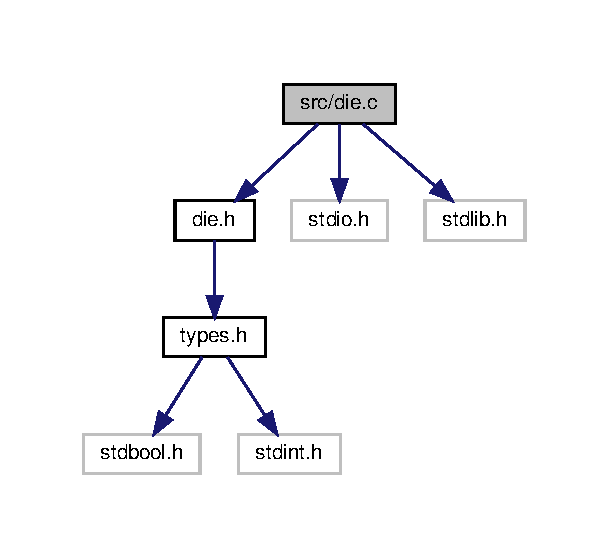
\includegraphics[width=292pt]{die_8c__incl}
\end{center}
\end{figure}
\subsection*{Data Structures}
\begin{DoxyCompactItemize}
\item 
struct \hyperlink{struct__Die}{\+\_\+\+Die}
\begin{DoxyCompactList}\small\item\em Die structure which contains information about Die. \end{DoxyCompactList}\end{DoxyCompactItemize}
\subsection*{Functions}
\begin{DoxyCompactItemize}
\item 
\hyperlink{struct__Die}{Die} $\ast$ \hyperlink{die_8c_a47b145c5793416cbb7adbe4e09cff3f7}{die\+\_\+init} (\hyperlink{types_8h_a845e604fb28f7e3d97549da3448149d3}{Id} id)
\begin{DoxyCompactList}\small\item\em Initializates a die. \end{DoxyCompactList}\item 
void \hyperlink{die_8c_a80d368f2c29bd18044c0f38fd0817bd6}{die\+\_\+destroy} (\hyperlink{struct__Die}{Die} $\ast$d)
\begin{DoxyCompactList}\small\item\em destroys a die \end{DoxyCompactList}\item 
int \hyperlink{die_8c_a4e2e6dd9a29d12c3b08dfa594879753e}{die\+\_\+roll} (\hyperlink{struct__Die}{Die} $\ast$d)
\begin{DoxyCompactList}\small\item\em rolls a die getting a random number \end{DoxyCompactList}\item 
const int \hyperlink{die_8c_a0ae47c02f343ffdbdf0750bb4864558b}{die\+\_\+get\+\_\+lastn} (\hyperlink{struct__Die}{Die} $\ast$die)
\begin{DoxyCompactList}\small\item\em gets the last random number of the die \end{DoxyCompactList}\end{DoxyCompactItemize}


\subsection{Detailed Description}
Die\textquotesingle{}s module dynamic. 

Defines functions responsible of constrolling a die

\begin{DoxyVersion}{Version}
0.\+0.\+3 
\end{DoxyVersion}
\begin{DoxyDate}{Date}
10/03/2019 
\end{DoxyDate}
\begin{DoxyAuthor}{Author}
Javier Romera 
\end{DoxyAuthor}
\begin{DoxyCopyright}{Copyright}
G\+NU Public License 
\end{DoxyCopyright}


\subsection{Function Documentation}
\mbox{\Hypertarget{die_8c_a47b145c5793416cbb7adbe4e09cff3f7}\label{die_8c_a47b145c5793416cbb7adbe4e09cff3f7}} 
\index{die.\+c@{die.\+c}!die\+\_\+init@{die\+\_\+init}}
\index{die\+\_\+init@{die\+\_\+init}!die.\+c@{die.\+c}}
\subsubsection{\texorpdfstring{die\+\_\+init()}{die\_init()}}
{\footnotesize\ttfamily \hyperlink{struct__Die}{Die}$\ast$ die\+\_\+init (\begin{DoxyParamCaption}\item[{\hyperlink{types_8h_a845e604fb28f7e3d97549da3448149d3}{Id}}]{id }\end{DoxyParamCaption})}



Initializates a die. 

\begin{DoxyAuthor}{Author}
Javier Romera 
\end{DoxyAuthor}

\begin{DoxyParams}{Parameters}
{\em \{\+Id\}} & id -\/ Die identification \\
\hline
\end{DoxyParams}

\begin{DoxyRetVals}{Return values}
{\em Returns} & a pointer towards die \\
\hline
\end{DoxyRetVals}
\mbox{\Hypertarget{die_8c_a80d368f2c29bd18044c0f38fd0817bd6}\label{die_8c_a80d368f2c29bd18044c0f38fd0817bd6}} 
\index{die.\+c@{die.\+c}!die\+\_\+destroy@{die\+\_\+destroy}}
\index{die\+\_\+destroy@{die\+\_\+destroy}!die.\+c@{die.\+c}}
\subsubsection{\texorpdfstring{die\+\_\+destroy()}{die\_destroy()}}
{\footnotesize\ttfamily void die\+\_\+destroy (\begin{DoxyParamCaption}\item[{\hyperlink{struct__Die}{Die} $\ast$}]{die }\end{DoxyParamCaption})}



destroys a die 

\begin{DoxyAuthor}{Author}
Javier Romera 
\end{DoxyAuthor}

\begin{DoxyParams}{Parameters}
{\em \{\+Die$\ast$\}} & die -\/ Die pointer \\
\hline
\end{DoxyParams}
\mbox{\Hypertarget{die_8c_a4e2e6dd9a29d12c3b08dfa594879753e}\label{die_8c_a4e2e6dd9a29d12c3b08dfa594879753e}} 
\index{die.\+c@{die.\+c}!die\+\_\+roll@{die\+\_\+roll}}
\index{die\+\_\+roll@{die\+\_\+roll}!die.\+c@{die.\+c}}
\subsubsection{\texorpdfstring{die\+\_\+roll()}{die\_roll()}}
{\footnotesize\ttfamily int die\+\_\+roll (\begin{DoxyParamCaption}\item[{\hyperlink{struct__Die}{Die} $\ast$}]{die }\end{DoxyParamCaption})}



rolls a die getting a random number 

\begin{DoxyAuthor}{Author}
Javier Romera 
\end{DoxyAuthor}

\begin{DoxyParams}{Parameters}
{\em \{\+Die$\ast$\}} & die -\/ Die pointer \\
\hline
\end{DoxyParams}

\begin{DoxyRetVals}{Return values}
{\em \{int\}} & -\/ Returns the random number; \\
\hline
\end{DoxyRetVals}
\mbox{\Hypertarget{die_8c_a0ae47c02f343ffdbdf0750bb4864558b}\label{die_8c_a0ae47c02f343ffdbdf0750bb4864558b}} 
\index{die.\+c@{die.\+c}!die\+\_\+get\+\_\+lastn@{die\+\_\+get\+\_\+lastn}}
\index{die\+\_\+get\+\_\+lastn@{die\+\_\+get\+\_\+lastn}!die.\+c@{die.\+c}}
\subsubsection{\texorpdfstring{die\+\_\+get\+\_\+lastn()}{die\_get\_lastn()}}
{\footnotesize\ttfamily const int die\+\_\+get\+\_\+lastn (\begin{DoxyParamCaption}\item[{\hyperlink{struct__Die}{Die} $\ast$}]{die }\end{DoxyParamCaption})}



gets the last random number of the die 

\begin{DoxyAuthor}{Author}
Javier Romera 
\end{DoxyAuthor}

\begin{DoxyParams}{Parameters}
{\em \{\+Die$\ast$\}} & die -\/ Die pointer \\
\hline
\end{DoxyParams}

\begin{DoxyRetVals}{Return values}
{\em \{int\}} & -\/ Returns the last random number; \\
\hline
\end{DoxyRetVals}

\hypertarget{g__engine_8c}{}\section{src/g\+\_\+engine.c File Reference}
\label{g__engine_8c}\index{src/g\+\_\+engine.\+c@{src/g\+\_\+engine.\+c}}


Graphic engine source code.  


{\ttfamily \#include \char`\"{}game.\+h\char`\"{}}\newline
{\ttfamily \#include \char`\"{}player.\+h\char`\"{}}\newline
{\ttfamily \#include \char`\"{}inventory.\+h\char`\"{}}\newline
{\ttfamily \#include \char`\"{}g\+\_\+engine.\+h\char`\"{}}\newline
{\ttfamily \#include \char`\"{}ui.\+h\char`\"{}}\newline
{\ttfamily \#include \char`\"{}link.\+h\char`\"{}}\newline
{\ttfamily \#include $<$stdio.\+h$>$}\newline
{\ttfamily \#include $<$stdlib.\+h$>$}\newline
{\ttfamily \#include $<$string.\+h$>$}\newline
{\ttfamily \#include $<$sys/time.\+h$>$}\newline
Include dependency graph for g\+\_\+engine.\+c\+:\nopagebreak
\begin{figure}[H]
\begin{center}
\leavevmode
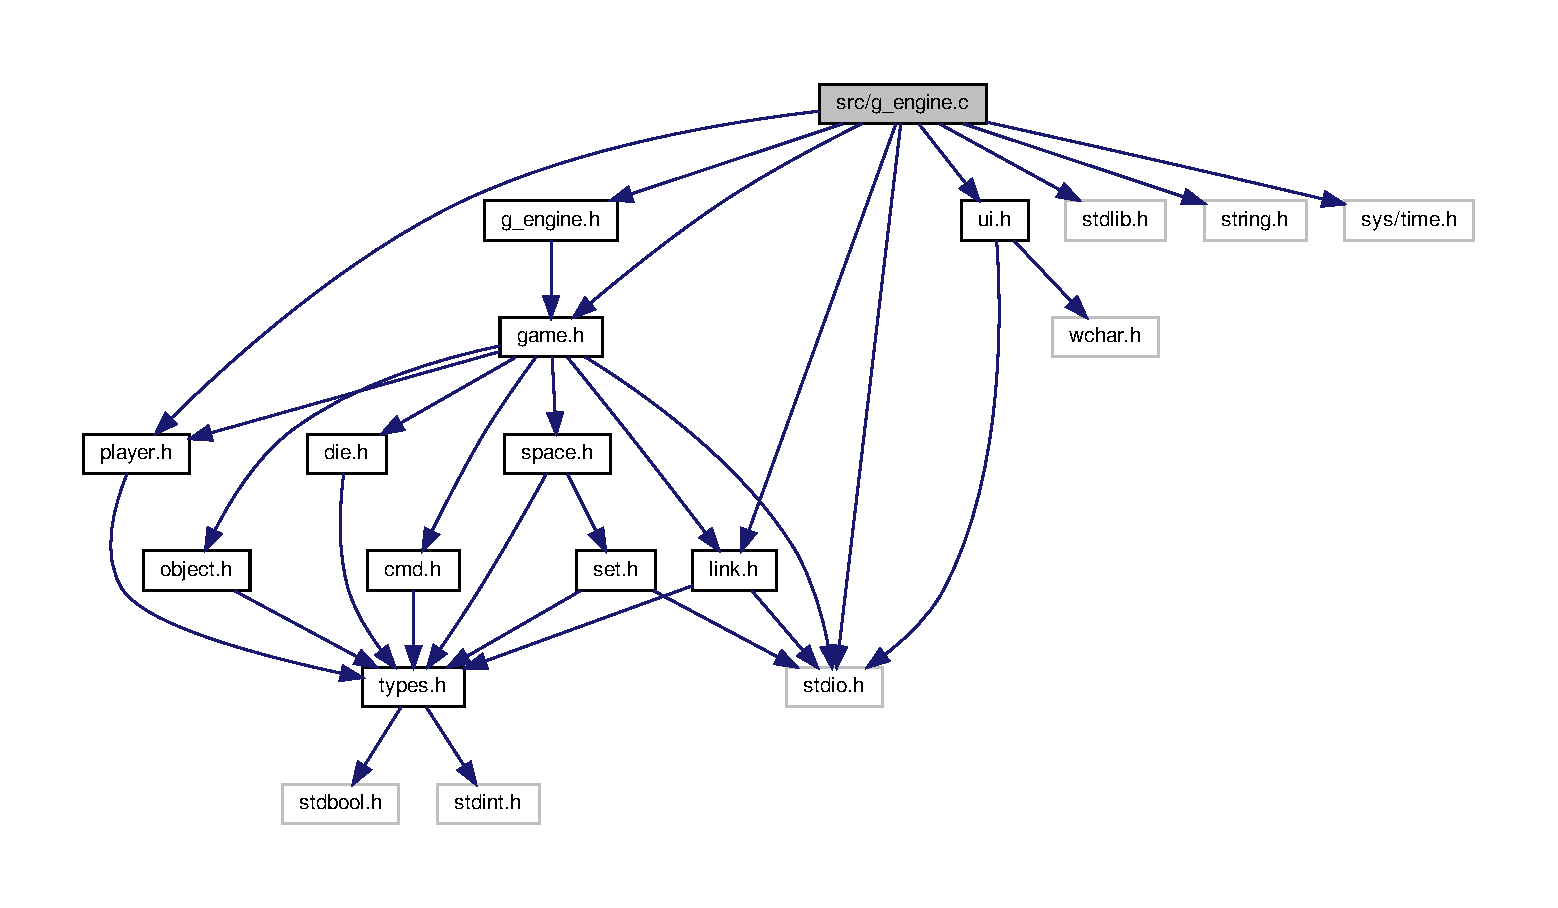
\includegraphics[width=350pt]{g__engine_8c__incl}
\end{center}
\end{figure}
\subsection*{Data Structures}
\begin{DoxyCompactItemize}
\item 
struct \hyperlink{struct__G__engine}{\+\_\+\+G\+\_\+engine}
\begin{DoxyCompactList}\small\item\em Main graphic engine structure. \end{DoxyCompactList}\end{DoxyCompactItemize}
\subsection*{Enumerations}
\begin{DoxyCompactItemize}
\item 
enum \hyperlink{g__engine_8c_a55884d4185031754f710955b5e32ebd9}{\+\_\+\+Boxes} \{ \newline
\hyperlink{g__engine_8c_a55884d4185031754f710955b5e32ebd9a82705894b9f5f3e3d088c69b4c0a41d5}{G\+A\+M\+E\+\_\+\+M\+AP}, 
\hyperlink{g__engine_8c_a55884d4185031754f710955b5e32ebd9a2f1db279e9c845748e9e4ef979f4471b}{G\+A\+M\+E\+\_\+\+O\+V\+E\+R\+V\+I\+EW}, 
\hyperlink{g__engine_8c_a55884d4185031754f710955b5e32ebd9a7c646ef62564b0dcc5e6653e223cfc52}{G\+A\+M\+E\+\_\+\+T\+I\+T\+LE}, 
\hyperlink{g__engine_8c_a55884d4185031754f710955b5e32ebd9ac49bda619a85c79a6be5bd102371c84d}{G\+A\+M\+E\+\_\+\+H\+E\+LP}, 
\newline
\hyperlink{g__engine_8c_a55884d4185031754f710955b5e32ebd9af3d3abc00730bab6971ebfa9608f1770}{G\+A\+M\+E\+\_\+\+F\+E\+ED}, 
\hyperlink{g__engine_8c_a55884d4185031754f710955b5e32ebd9a4c9c8637f3b906daa4173fe12bd95e7d}{G\+A\+M\+E\+\_\+\+I\+N\+FO}, 
\hyperlink{g__engine_8c_a55884d4185031754f710955b5e32ebd9a02d9fd1e8fff421c9c3bf1c0cd108171}{H\+E\+L\+P\+\_\+\+T\+I\+T\+LE}, 
\hyperlink{g__engine_8c_a55884d4185031754f710955b5e32ebd9ad585f458456d9720cec9aa4d845ecd93}{H\+E\+L\+P\+\_\+\+B\+O\+DY}
 \}
\end{DoxyCompactItemize}
\subsection*{Functions}
\begin{DoxyCompactItemize}
\item 
void \hyperlink{g__engine_8c_a947f9e2e4c31ea006fd0c69072c9abf3}{parse\+\_\+space} (\hyperlink{struct__Game}{Game} $\ast$game, \hyperlink{struct__G__engine}{G\+\_\+engine} $\ast$ge, \hyperlink{space_8h_a67533ffc2b70463baecc38fb0629bbfc}{Space} $\ast$sp, int id, int x, int y)
\begin{DoxyCompactList}\small\item\em Parses a given space. \end{DoxyCompactList}\item 
\hyperlink{struct__G__engine}{G\+\_\+engine} $\ast$ \hyperlink{g__engine_8c_aa2f5a0548ea6fedb671c594d4f0cf039}{g\+\_\+engine\+\_\+create} ()
\begin{DoxyCompactList}\small\item\em Creates a new graphic engine. \end{DoxyCompactList}\item 
void \hyperlink{g__engine_8c_a22856c5bd4a0185424313f9fcb5ed4d7}{g\+\_\+engine\+\_\+paint\+\_\+help} (\hyperlink{struct__G__engine}{G\+\_\+engine} $\ast$ge, \hyperlink{struct__Game}{Game} $\ast$game)
\begin{DoxyCompactList}\small\item\em Draws the help interface. \end{DoxyCompactList}\item 
void \hyperlink{g__engine_8c_ae61d1ed693a2bfc2967b4550fc128536}{g\+\_\+engine\+\_\+destroy} (\hyperlink{struct__G__engine}{G\+\_\+engine} $\ast$ge)
\begin{DoxyCompactList}\small\item\em Destroys a graphic engine. \end{DoxyCompactList}\item 
void \hyperlink{g__engine_8c_ab215509a5b24333ada8465e80df43387}{g\+\_\+engine\+\_\+paint\+\_\+game} (\hyperlink{struct__G__engine}{G\+\_\+engine} $\ast$ge, \hyperlink{struct__Game}{Game} $\ast$game)
\begin{DoxyCompactList}\small\item\em Draws the game interface. \end{DoxyCompactList}\end{DoxyCompactItemize}


\subsection{Detailed Description}
Graphic engine source code. 

\begin{DoxyVersion}{Version}
0.\+7.\+2 
\end{DoxyVersion}
\begin{DoxyDate}{Date}
17/03/2019 
\end{DoxyDate}
\begin{DoxyCopyright}{Copyright}
G\+NU Public License 
\end{DoxyCopyright}


\subsection{Enumeration Type Documentation}
\mbox{\Hypertarget{g__engine_8c_a55884d4185031754f710955b5e32ebd9}\label{g__engine_8c_a55884d4185031754f710955b5e32ebd9}} 
\index{g\+\_\+engine.\+c@{g\+\_\+engine.\+c}!\+\_\+\+Boxes@{\+\_\+\+Boxes}}
\index{\+\_\+\+Boxes@{\+\_\+\+Boxes}!g\+\_\+engine.\+c@{g\+\_\+engine.\+c}}
\subsubsection{\texorpdfstring{\+\_\+\+Boxes}{\_Boxes}}
{\footnotesize\ttfamily enum \hyperlink{g__engine_8c_a55884d4185031754f710955b5e32ebd9}{\+\_\+\+Boxes}}

Box list \begin{DoxyEnumFields}{Enumerator}
\raisebox{\heightof{T}}[0pt][0pt]{\index{G\+A\+M\+E\+\_\+\+M\+AP@{G\+A\+M\+E\+\_\+\+M\+AP}!g\+\_\+engine.\+c@{g\+\_\+engine.\+c}}\index{g\+\_\+engine.\+c@{g\+\_\+engine.\+c}!G\+A\+M\+E\+\_\+\+M\+AP@{G\+A\+M\+E\+\_\+\+M\+AP}}}\mbox{\Hypertarget{g__engine_8c_a55884d4185031754f710955b5e32ebd9a82705894b9f5f3e3d088c69b4c0a41d5}\label{g__engine_8c_a55884d4185031754f710955b5e32ebd9a82705894b9f5f3e3d088c69b4c0a41d5}} 
G\+A\+M\+E\+\_\+\+M\+AP&Map box \\
\hline

\raisebox{\heightof{T}}[0pt][0pt]{\index{G\+A\+M\+E\+\_\+\+O\+V\+E\+R\+V\+I\+EW@{G\+A\+M\+E\+\_\+\+O\+V\+E\+R\+V\+I\+EW}!g\+\_\+engine.\+c@{g\+\_\+engine.\+c}}\index{g\+\_\+engine.\+c@{g\+\_\+engine.\+c}!G\+A\+M\+E\+\_\+\+O\+V\+E\+R\+V\+I\+EW@{G\+A\+M\+E\+\_\+\+O\+V\+E\+R\+V\+I\+EW}}}\mbox{\Hypertarget{g__engine_8c_a55884d4185031754f710955b5e32ebd9a2f1db279e9c845748e9e4ef979f4471b}\label{g__engine_8c_a55884d4185031754f710955b5e32ebd9a2f1db279e9c845748e9e4ef979f4471b}} 
G\+A\+M\+E\+\_\+\+O\+V\+E\+R\+V\+I\+EW&Overview box \\
\hline

\raisebox{\heightof{T}}[0pt][0pt]{\index{G\+A\+M\+E\+\_\+\+T\+I\+T\+LE@{G\+A\+M\+E\+\_\+\+T\+I\+T\+LE}!g\+\_\+engine.\+c@{g\+\_\+engine.\+c}}\index{g\+\_\+engine.\+c@{g\+\_\+engine.\+c}!G\+A\+M\+E\+\_\+\+T\+I\+T\+LE@{G\+A\+M\+E\+\_\+\+T\+I\+T\+LE}}}\mbox{\Hypertarget{g__engine_8c_a55884d4185031754f710955b5e32ebd9a7c646ef62564b0dcc5e6653e223cfc52}\label{g__engine_8c_a55884d4185031754f710955b5e32ebd9a7c646ef62564b0dcc5e6653e223cfc52}} 
G\+A\+M\+E\+\_\+\+T\+I\+T\+LE&Title box \\
\hline

\raisebox{\heightof{T}}[0pt][0pt]{\index{G\+A\+M\+E\+\_\+\+H\+E\+LP@{G\+A\+M\+E\+\_\+\+H\+E\+LP}!g\+\_\+engine.\+c@{g\+\_\+engine.\+c}}\index{g\+\_\+engine.\+c@{g\+\_\+engine.\+c}!G\+A\+M\+E\+\_\+\+H\+E\+LP@{G\+A\+M\+E\+\_\+\+H\+E\+LP}}}\mbox{\Hypertarget{g__engine_8c_a55884d4185031754f710955b5e32ebd9ac49bda619a85c79a6be5bd102371c84d}\label{g__engine_8c_a55884d4185031754f710955b5e32ebd9ac49bda619a85c79a6be5bd102371c84d}} 
G\+A\+M\+E\+\_\+\+H\+E\+LP&Help box \\
\hline

\raisebox{\heightof{T}}[0pt][0pt]{\index{G\+A\+M\+E\+\_\+\+F\+E\+ED@{G\+A\+M\+E\+\_\+\+F\+E\+ED}!g\+\_\+engine.\+c@{g\+\_\+engine.\+c}}\index{g\+\_\+engine.\+c@{g\+\_\+engine.\+c}!G\+A\+M\+E\+\_\+\+F\+E\+ED@{G\+A\+M\+E\+\_\+\+F\+E\+ED}}}\mbox{\Hypertarget{g__engine_8c_a55884d4185031754f710955b5e32ebd9af3d3abc00730bab6971ebfa9608f1770}\label{g__engine_8c_a55884d4185031754f710955b5e32ebd9af3d3abc00730bab6971ebfa9608f1770}} 
G\+A\+M\+E\+\_\+\+F\+E\+ED&Feedback box \\
\hline

\raisebox{\heightof{T}}[0pt][0pt]{\index{G\+A\+M\+E\+\_\+\+I\+N\+FO@{G\+A\+M\+E\+\_\+\+I\+N\+FO}!g\+\_\+engine.\+c@{g\+\_\+engine.\+c}}\index{g\+\_\+engine.\+c@{g\+\_\+engine.\+c}!G\+A\+M\+E\+\_\+\+I\+N\+FO@{G\+A\+M\+E\+\_\+\+I\+N\+FO}}}\mbox{\Hypertarget{g__engine_8c_a55884d4185031754f710955b5e32ebd9a4c9c8637f3b906daa4173fe12bd95e7d}\label{g__engine_8c_a55884d4185031754f710955b5e32ebd9a4c9c8637f3b906daa4173fe12bd95e7d}} 
G\+A\+M\+E\+\_\+\+I\+N\+FO&Info box \\
\hline

\raisebox{\heightof{T}}[0pt][0pt]{\index{H\+E\+L\+P\+\_\+\+T\+I\+T\+LE@{H\+E\+L\+P\+\_\+\+T\+I\+T\+LE}!g\+\_\+engine.\+c@{g\+\_\+engine.\+c}}\index{g\+\_\+engine.\+c@{g\+\_\+engine.\+c}!H\+E\+L\+P\+\_\+\+T\+I\+T\+LE@{H\+E\+L\+P\+\_\+\+T\+I\+T\+LE}}}\mbox{\Hypertarget{g__engine_8c_a55884d4185031754f710955b5e32ebd9a02d9fd1e8fff421c9c3bf1c0cd108171}\label{g__engine_8c_a55884d4185031754f710955b5e32ebd9a02d9fd1e8fff421c9c3bf1c0cd108171}} 
H\+E\+L\+P\+\_\+\+T\+I\+T\+LE&Help title \\
\hline

\raisebox{\heightof{T}}[0pt][0pt]{\index{H\+E\+L\+P\+\_\+\+B\+O\+DY@{H\+E\+L\+P\+\_\+\+B\+O\+DY}!g\+\_\+engine.\+c@{g\+\_\+engine.\+c}}\index{g\+\_\+engine.\+c@{g\+\_\+engine.\+c}!H\+E\+L\+P\+\_\+\+B\+O\+DY@{H\+E\+L\+P\+\_\+\+B\+O\+DY}}}\mbox{\Hypertarget{g__engine_8c_a55884d4185031754f710955b5e32ebd9ad585f458456d9720cec9aa4d845ecd93}\label{g__engine_8c_a55884d4185031754f710955b5e32ebd9ad585f458456d9720cec9aa4d845ecd93}} 
H\+E\+L\+P\+\_\+\+B\+O\+DY&Help body \\
\hline

\end{DoxyEnumFields}


\subsection{Function Documentation}
\mbox{\Hypertarget{g__engine_8c_a947f9e2e4c31ea006fd0c69072c9abf3}\label{g__engine_8c_a947f9e2e4c31ea006fd0c69072c9abf3}} 
\index{g\+\_\+engine.\+c@{g\+\_\+engine.\+c}!parse\+\_\+space@{parse\+\_\+space}}
\index{parse\+\_\+space@{parse\+\_\+space}!g\+\_\+engine.\+c@{g\+\_\+engine.\+c}}
\subsubsection{\texorpdfstring{parse\+\_\+space()}{parse\_space()}}
{\footnotesize\ttfamily void parse\+\_\+space (\begin{DoxyParamCaption}\item[{\hyperlink{struct__Game}{Game} $\ast$}]{game,  }\item[{\hyperlink{struct__G__engine}{G\+\_\+engine} $\ast$}]{ge,  }\item[{\hyperlink{space_8h_a67533ffc2b70463baecc38fb0629bbfc}{Space} $\ast$}]{sp,  }\item[{int}]{id,  }\item[{int}]{x,  }\item[{int}]{y }\end{DoxyParamCaption})}



Parses a given space. 


\begin{DoxyParams}{Parameters}
{\em \{\+Game$\ast$\}} & game -\/ Game pointer \\
\hline
{\em \{\+G\+\_\+engine$\ast$\}} & ge -\/ Graphic engine pointer \\
\hline
{\em \{\+Space$\ast$\}} & sp -\/ Space to be drawn \\
\hline
{\em \{int\}} & id -\/ Box id \\
\hline
{\em \{int\}} & x -\/ Begin x position (relative to the box) \\
\hline
{\em \{int\}} & y -\/ Begin y position (relative to the box) \\
\hline
\end{DoxyParams}
\mbox{\Hypertarget{g__engine_8c_aa2f5a0548ea6fedb671c594d4f0cf039}\label{g__engine_8c_aa2f5a0548ea6fedb671c594d4f0cf039}} 
\index{g\+\_\+engine.\+c@{g\+\_\+engine.\+c}!g\+\_\+engine\+\_\+create@{g\+\_\+engine\+\_\+create}}
\index{g\+\_\+engine\+\_\+create@{g\+\_\+engine\+\_\+create}!g\+\_\+engine.\+c@{g\+\_\+engine.\+c}}
\subsubsection{\texorpdfstring{g\+\_\+engine\+\_\+create()}{g\_engine\_create()}}
{\footnotesize\ttfamily \hyperlink{struct__G__engine}{G\+\_\+engine}$\ast$ g\+\_\+engine\+\_\+create (\begin{DoxyParamCaption}{ }\end{DoxyParamCaption})}



Creates a new graphic engine. 


\begin{DoxyRetVals}{Return values}
{\em \{\+G\+\_\+engine$\ast$\}} & -\/ Returns a graphic engine pointer \\
\hline
\end{DoxyRetVals}
\mbox{\Hypertarget{g__engine_8c_a22856c5bd4a0185424313f9fcb5ed4d7}\label{g__engine_8c_a22856c5bd4a0185424313f9fcb5ed4d7}} 
\index{g\+\_\+engine.\+c@{g\+\_\+engine.\+c}!g\+\_\+engine\+\_\+paint\+\_\+help@{g\+\_\+engine\+\_\+paint\+\_\+help}}
\index{g\+\_\+engine\+\_\+paint\+\_\+help@{g\+\_\+engine\+\_\+paint\+\_\+help}!g\+\_\+engine.\+c@{g\+\_\+engine.\+c}}
\subsubsection{\texorpdfstring{g\+\_\+engine\+\_\+paint\+\_\+help()}{g\_engine\_paint\_help()}}
{\footnotesize\ttfamily void g\+\_\+engine\+\_\+paint\+\_\+help (\begin{DoxyParamCaption}\item[{\hyperlink{struct__G__engine}{G\+\_\+engine} $\ast$}]{ge,  }\item[{\hyperlink{struct__Game}{Game} $\ast$}]{game }\end{DoxyParamCaption})}



Draws the help interface. 


\begin{DoxyParams}{Parameters}
{\em \{\+G\+\_\+engine$\ast$\}} & ge -\/ Graphic engine pointer \\
\hline
{\em \{\+Game$\ast$\}} & game -\/ Game pointer \\
\hline
\end{DoxyParams}
\mbox{\Hypertarget{g__engine_8c_ae61d1ed693a2bfc2967b4550fc128536}\label{g__engine_8c_ae61d1ed693a2bfc2967b4550fc128536}} 
\index{g\+\_\+engine.\+c@{g\+\_\+engine.\+c}!g\+\_\+engine\+\_\+destroy@{g\+\_\+engine\+\_\+destroy}}
\index{g\+\_\+engine\+\_\+destroy@{g\+\_\+engine\+\_\+destroy}!g\+\_\+engine.\+c@{g\+\_\+engine.\+c}}
\subsubsection{\texorpdfstring{g\+\_\+engine\+\_\+destroy()}{g\_engine\_destroy()}}
{\footnotesize\ttfamily void g\+\_\+engine\+\_\+destroy (\begin{DoxyParamCaption}\item[{\hyperlink{struct__G__engine}{G\+\_\+engine} $\ast$}]{ge }\end{DoxyParamCaption})}



Destroys a graphic engine. 


\begin{DoxyParams}{Parameters}
{\em \{\+G\+\_\+engine$\ast$\}} & ge -\/ Graphic engine pointer \\
\hline
\end{DoxyParams}
\mbox{\Hypertarget{g__engine_8c_ab215509a5b24333ada8465e80df43387}\label{g__engine_8c_ab215509a5b24333ada8465e80df43387}} 
\index{g\+\_\+engine.\+c@{g\+\_\+engine.\+c}!g\+\_\+engine\+\_\+paint\+\_\+game@{g\+\_\+engine\+\_\+paint\+\_\+game}}
\index{g\+\_\+engine\+\_\+paint\+\_\+game@{g\+\_\+engine\+\_\+paint\+\_\+game}!g\+\_\+engine.\+c@{g\+\_\+engine.\+c}}
\subsubsection{\texorpdfstring{g\+\_\+engine\+\_\+paint\+\_\+game()}{g\_engine\_paint\_game()}}
{\footnotesize\ttfamily void g\+\_\+engine\+\_\+paint\+\_\+game (\begin{DoxyParamCaption}\item[{\hyperlink{struct__G__engine}{G\+\_\+engine} $\ast$}]{ge,  }\item[{\hyperlink{struct__Game}{Game} $\ast$}]{game }\end{DoxyParamCaption})}



Draws the game interface. 


\begin{DoxyParams}{Parameters}
{\em \{\+G\+\_\+engine$\ast$\}} & ge -\/ Graphic engine pointer \\
\hline
{\em \{\+Game$\ast$\}} & game -\/ Game pointer \\
\hline
\end{DoxyParams}

\hypertarget{game__loop_8c}{}\section{src/game\+\_\+loop.c File Reference}
\label{game__loop_8c}\index{src/game\+\_\+loop.\+c@{src/game\+\_\+loop.\+c}}


Main game loop.  


{\ttfamily \#include \char`\"{}g\+\_\+engine.\+h\char`\"{}}\newline
{\ttfamily \#include \char`\"{}types.\+h\char`\"{}}\newline
{\ttfamily \#include \char`\"{}log.\+h\char`\"{}}\newline
{\ttfamily \#include $<$stdio.\+h$>$}\newline
{\ttfamily \#include $<$stdlib.\+h$>$}\newline
{\ttfamily \#include $<$time.\+h$>$}\newline
{\ttfamily \#include $<$string.\+h$>$}\newline
{\ttfamily \#include $<$signal.\+h$>$}\newline
{\ttfamily \#include $<$locale.\+h$>$}\newline
{\ttfamily \#include $<$unistd.\+h$>$}\newline
Include dependency graph for game\+\_\+loop.\+c\+:
\nopagebreak
\begin{figure}[H]
\begin{center}
\leavevmode
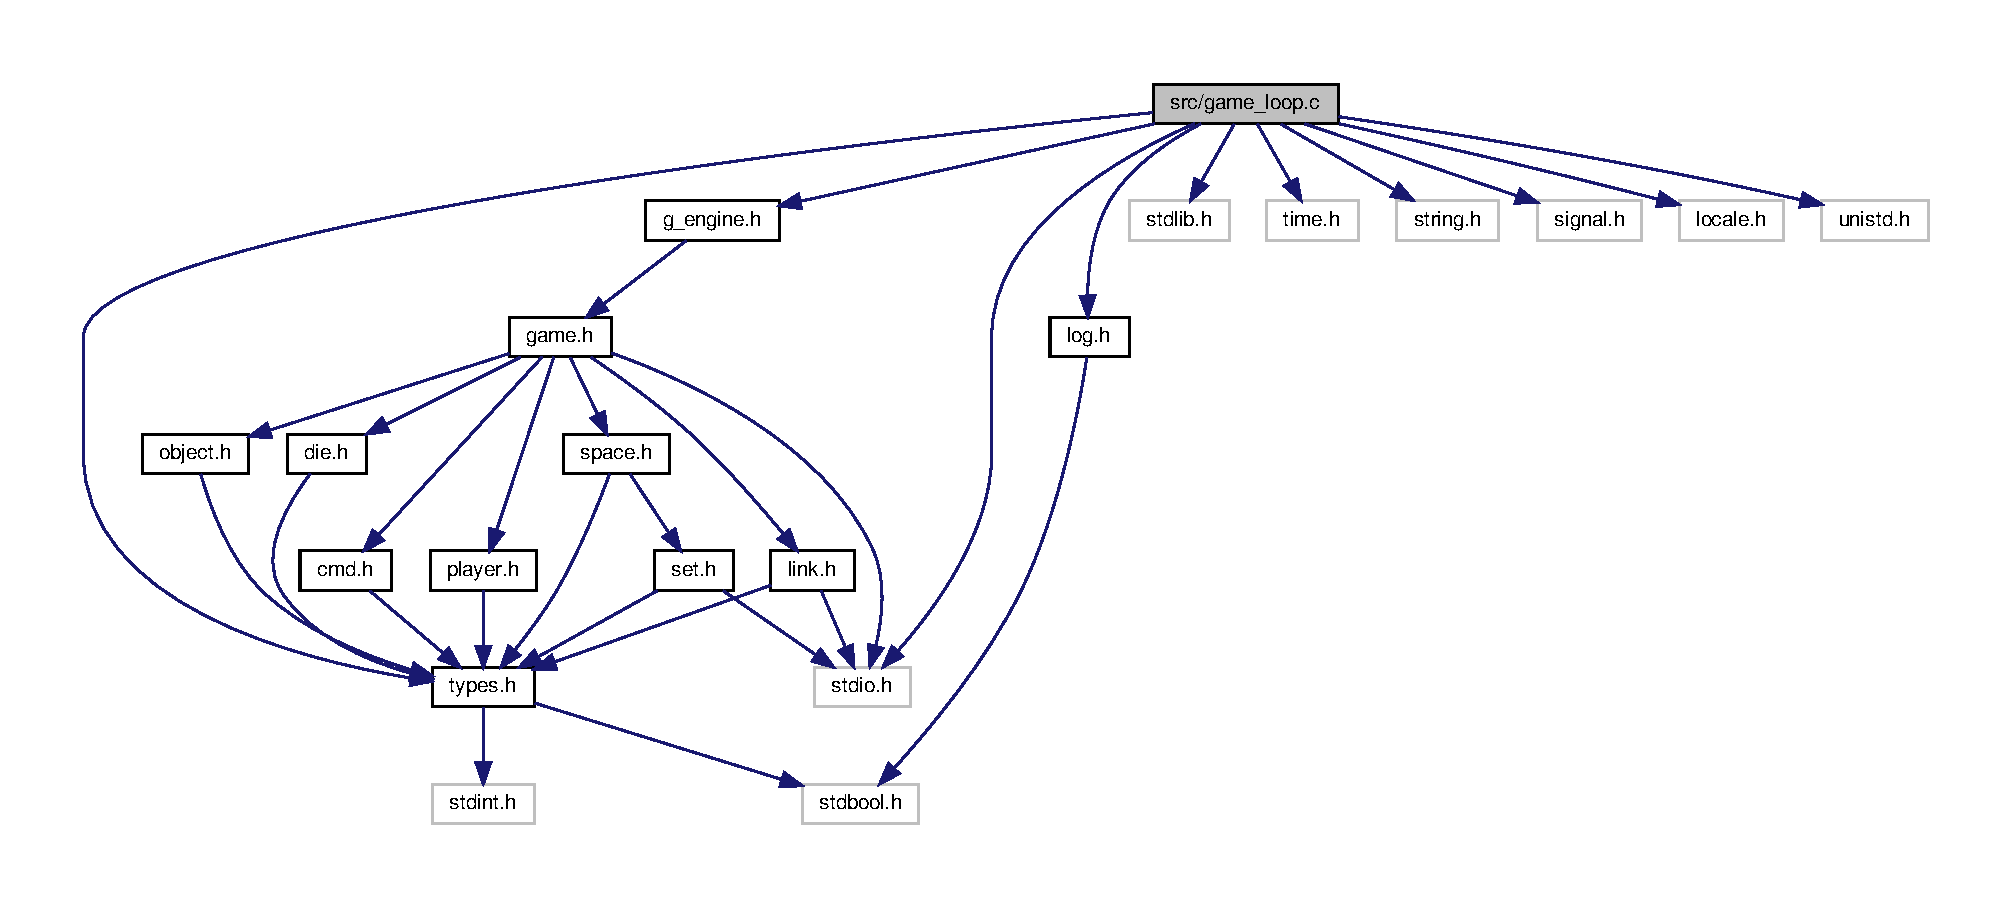
\includegraphics[width=350pt]{game__loop_8c__incl}
\end{center}
\end{figure}
\subsection*{Functions}
\begin{DoxyCompactItemize}
\item 
void \hyperlink{game__loop_8c_ac2aeadb517220b0bdc34fe1963ef4d9f}{ctrl\+\_\+c} ()
\begin{DoxyCompactList}\small\item\em This function will be executed when a signal is dispatched. \end{DoxyCompactList}\item 
void \hyperlink{game__loop_8c_acca7de49935d305a8dc26faa07d53706}{\+\_\+kill} (int errc)
\begin{DoxyCompactList}\small\item\em This function will free all the memory. \end{DoxyCompactList}\item 
\mbox{\Hypertarget{game__loop_8c_a0ddf1224851353fc92bfbff6f499fa97}\label{game__loop_8c_a0ddf1224851353fc92bfbff6f499fa97}} 
int {\bfseries main} (int argc, char $\ast$argv\mbox{[}$\,$\mbox{]})
\end{DoxyCompactItemize}
\subsection*{Variables}
\begin{DoxyCompactItemize}
\item 
\mbox{\Hypertarget{game__loop_8c_a58bdb5643d0814ac4e697a1564b79b70}\label{game__loop_8c_a58bdb5643d0814ac4e697a1564b79b70}} 
\hyperlink{struct__Game}{Game} $\ast$ {\bfseries game}
\item 
\mbox{\Hypertarget{game__loop_8c_a01956169a8ec25a149bc0130df54e3d8}\label{game__loop_8c_a01956169a8ec25a149bc0130df54e3d8}} 
\hyperlink{struct__G__engine}{G\+\_\+engine} $\ast$ {\bfseries gengine}
\end{DoxyCompactItemize}


\subsection{Detailed Description}
Main game loop. 

\begin{DoxyAuthor}{Author}
Álvaro Rodríguez \& Javier Romera 
\end{DoxyAuthor}
\begin{DoxyVersion}{Version}
1.\+0 
\end{DoxyVersion}
\begin{DoxyDate}{Date}
07/02/2019 
\end{DoxyDate}
\begin{DoxyCopyright}{Copyright}
G\+NU Public License 
\end{DoxyCopyright}


\subsection{Function Documentation}
\mbox{\Hypertarget{game__loop_8c_ac2aeadb517220b0bdc34fe1963ef4d9f}\label{game__loop_8c_ac2aeadb517220b0bdc34fe1963ef4d9f}} 
\index{game\+\_\+loop.\+c@{game\+\_\+loop.\+c}!ctrl\+\_\+c@{ctrl\+\_\+c}}
\index{ctrl\+\_\+c@{ctrl\+\_\+c}!game\+\_\+loop.\+c@{game\+\_\+loop.\+c}}
\subsubsection{\texorpdfstring{ctrl\+\_\+c()}{ctrl\_c()}}
{\footnotesize\ttfamily void ctrl\+\_\+c (\begin{DoxyParamCaption}{ }\end{DoxyParamCaption})}



This function will be executed when a signal is dispatched. 


\begin{DoxyParams}{Parameters}
{\em \{int\}} & sign -\/ Signal id \\
\hline
\end{DoxyParams}
\mbox{\Hypertarget{game__loop_8c_acca7de49935d305a8dc26faa07d53706}\label{game__loop_8c_acca7de49935d305a8dc26faa07d53706}} 
\index{game\+\_\+loop.\+c@{game\+\_\+loop.\+c}!\+\_\+kill@{\+\_\+kill}}
\index{\+\_\+kill@{\+\_\+kill}!game\+\_\+loop.\+c@{game\+\_\+loop.\+c}}
\subsubsection{\texorpdfstring{\+\_\+kill()}{\_kill()}}
{\footnotesize\ttfamily void \+\_\+kill (\begin{DoxyParamCaption}\item[{int}]{errc }\end{DoxyParamCaption})}



This function will free all the memory. 


\begin{DoxyParams}{Parameters}
{\em \{int\}} & errc -\/ Error code \\
\hline
\end{DoxyParams}

\hypertarget{inventory_8c}{}\section{src/inventory.c File Reference}
\label{inventory_8c}\index{src/inventory.\+c@{src/inventory.\+c}}


Code implementation of the inventory manager.  


{\ttfamily \#include $<$stdio.\+h$>$}\newline
{\ttfamily \#include $<$stdlib.\+h$>$}\newline
{\ttfamily \#include \char`\"{}set.\+h\char`\"{}}\newline
{\ttfamily \#include \char`\"{}inventory.\+h\char`\"{}}\newline
Include dependency graph for inventory.\+c\+:\nopagebreak
\begin{figure}[H]
\begin{center}
\leavevmode
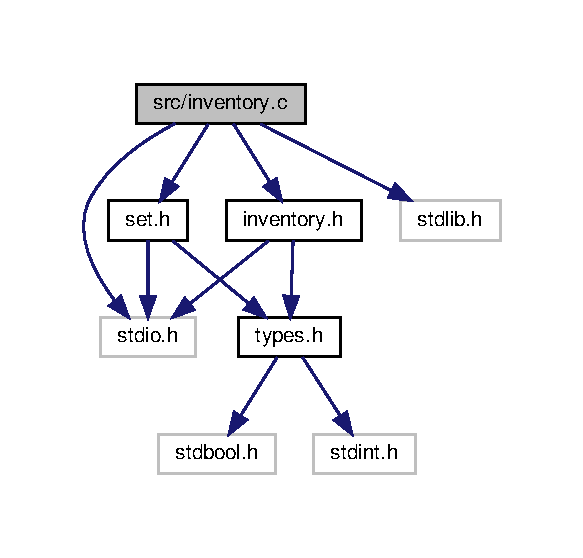
\includegraphics[width=280pt]{inventory_8c__incl}
\end{center}
\end{figure}
\subsection*{Data Structures}
\begin{DoxyCompactItemize}
\item 
struct \hyperlink{struct__Inventory}{\+\_\+\+Inventory}
\end{DoxyCompactItemize}
\subsection*{Functions}
\begin{DoxyCompactItemize}
\item 
\hyperlink{inventory_8h_a2253bf64ac4ce6a9c1d6f39c0b0d32a3}{Inventory} $\ast$ \hyperlink{inventory_8c_a5d6b47f7a727932c56d66a65fb540910}{inventory\+\_\+create} ()
\begin{DoxyCompactList}\small\item\em This fuction initializes an inventory. \end{DoxyCompactList}\item 
void \hyperlink{inventory_8c_a90250adb627aaa1305954287a9154966}{inventory\+\_\+destroy} (\hyperlink{inventory_8h_a2253bf64ac4ce6a9c1d6f39c0b0d32a3}{Inventory} $\ast$inv)
\begin{DoxyCompactList}\small\item\em This fuction destroys an Inventory. \end{DoxyCompactList}\item 
\hyperlink{types_8h_a32c27cc471df37f4fc818d65de0a56c4}{S\+T\+A\+T\+US} \hyperlink{inventory_8c_a91549cebec2fd5c6f3ec0c7d6448dc31}{inventory\+\_\+add\+\_\+id} (\hyperlink{inventory_8h_a2253bf64ac4ce6a9c1d6f39c0b0d32a3}{Inventory} $\ast$inv, \hyperlink{types_8h_a845e604fb28f7e3d97549da3448149d3}{Id} id)
\begin{DoxyCompactList}\small\item\em Adds a new id to an inventory. \end{DoxyCompactList}\item 
\hyperlink{types_8h_a32c27cc471df37f4fc818d65de0a56c4}{S\+T\+A\+T\+US} \hyperlink{inventory_8c_abfdd9b2876ee540ae426bfb5b200bf3c}{inventory\+\_\+del\+\_\+id} (\hyperlink{inventory_8h_a2253bf64ac4ce6a9c1d6f39c0b0d32a3}{Inventory} $\ast$inv, \hyperlink{types_8h_a845e604fb28f7e3d97549da3448149d3}{Id} id)
\begin{DoxyCompactList}\small\item\em Deletes an id from an inventory. \end{DoxyCompactList}\item 
bool \hyperlink{inventory_8c_aebb90d4c533fbf389e77df3987b6e76d}{inventory\+\_\+has\+\_\+id} (\hyperlink{inventory_8h_a2253bf64ac4ce6a9c1d6f39c0b0d32a3}{Inventory} $\ast$inv, \hyperlink{types_8h_a845e604fb28f7e3d97549da3448149d3}{Id} id)
\begin{DoxyCompactList}\small\item\em Tells if an id is in a Inventory or not. \end{DoxyCompactList}\item 
int \hyperlink{inventory_8c_aa1391bde411c1726b2d8fc23de1d18b9}{inventory\+\_\+get\+\_\+total} (\hyperlink{inventory_8h_a2253bf64ac4ce6a9c1d6f39c0b0d32a3}{Inventory} $\ast$inv)
\begin{DoxyCompactList}\small\item\em Tells the number of id\textquotesingle{}s in an inventory. \end{DoxyCompactList}\item 
int \hyperlink{inventory_8c_a9ea9977c26995708d271af60ad96650b}{inventory\+\_\+get\+\_\+max} (\hyperlink{inventory_8h_a2253bf64ac4ce6a9c1d6f39c0b0d32a3}{Inventory} $\ast$inv)
\begin{DoxyCompactList}\small\item\em Tells the maximun capacity of the Inventory. \end{DoxyCompactList}\item 
bool \hyperlink{inventory_8c_a913ebf717a79dced571ff9aad64352b5}{inventory\+\_\+is\+\_\+full} (\hyperlink{inventory_8h_a2253bf64ac4ce6a9c1d6f39c0b0d32a3}{Inventory} $\ast$inv)
\begin{DoxyCompactList}\small\item\em Tells if an inventory is full or not. \end{DoxyCompactList}\item 
bool \hyperlink{inventory_8c_aaa1a7e022c311412859a6a588b7c78fe}{inventory\+\_\+is\+\_\+empty} (\hyperlink{inventory_8h_a2253bf64ac4ce6a9c1d6f39c0b0d32a3}{Inventory} $\ast$inv)
\begin{DoxyCompactList}\small\item\em Tells if an inventory is empty or not. \end{DoxyCompactList}\end{DoxyCompactItemize}


\subsection{Detailed Description}
Code implementation of the inventory manager. 

\begin{DoxyDate}{Date}
07/04/2019 
\end{DoxyDate}


\subsection{Function Documentation}
\mbox{\Hypertarget{inventory_8c_a5d6b47f7a727932c56d66a65fb540910}\label{inventory_8c_a5d6b47f7a727932c56d66a65fb540910}} 
\index{inventory.\+c@{inventory.\+c}!inventory\+\_\+create@{inventory\+\_\+create}}
\index{inventory\+\_\+create@{inventory\+\_\+create}!inventory.\+c@{inventory.\+c}}
\subsubsection{\texorpdfstring{inventory\+\_\+create()}{inventory\_create()}}
{\footnotesize\ttfamily \hyperlink{inventory_8h_a2253bf64ac4ce6a9c1d6f39c0b0d32a3}{Inventory}$\ast$ inventory\+\_\+create (\begin{DoxyParamCaption}{ }\end{DoxyParamCaption})}



This fuction initializes an inventory. 

\begin{DoxyAuthor}{Author}
Miguel Rodríguez
\end{DoxyAuthor}

\begin{DoxyRetVals}{Return values}
{\em \{\+Inventory$\ast$\}} & -\/ Returns an inventory\textquotesingle{}s pointer \\
\hline
\end{DoxyRetVals}
\mbox{\Hypertarget{inventory_8c_a90250adb627aaa1305954287a9154966}\label{inventory_8c_a90250adb627aaa1305954287a9154966}} 
\index{inventory.\+c@{inventory.\+c}!inventory\+\_\+destroy@{inventory\+\_\+destroy}}
\index{inventory\+\_\+destroy@{inventory\+\_\+destroy}!inventory.\+c@{inventory.\+c}}
\subsubsection{\texorpdfstring{inventory\+\_\+destroy()}{inventory\_destroy()}}
{\footnotesize\ttfamily void inventory\+\_\+destroy (\begin{DoxyParamCaption}\item[{\hyperlink{inventory_8h_a2253bf64ac4ce6a9c1d6f39c0b0d32a3}{Inventory} $\ast$}]{inv }\end{DoxyParamCaption})}



This fuction destroys an Inventory. 

\begin{DoxyAuthor}{Author}
Miguel Rodríguez 
\end{DoxyAuthor}

\begin{DoxyParams}{Parameters}
{\em \{\+Inventory$\ast$\}} & inv -\/ Inventory pointer \\
\hline
\end{DoxyParams}
\mbox{\Hypertarget{inventory_8c_a91549cebec2fd5c6f3ec0c7d6448dc31}\label{inventory_8c_a91549cebec2fd5c6f3ec0c7d6448dc31}} 
\index{inventory.\+c@{inventory.\+c}!inventory\+\_\+add\+\_\+id@{inventory\+\_\+add\+\_\+id}}
\index{inventory\+\_\+add\+\_\+id@{inventory\+\_\+add\+\_\+id}!inventory.\+c@{inventory.\+c}}
\subsubsection{\texorpdfstring{inventory\+\_\+add\+\_\+id()}{inventory\_add\_id()}}
{\footnotesize\ttfamily \hyperlink{types_8h_a32c27cc471df37f4fc818d65de0a56c4}{S\+T\+A\+T\+US} inventory\+\_\+add\+\_\+id (\begin{DoxyParamCaption}\item[{\hyperlink{inventory_8h_a2253bf64ac4ce6a9c1d6f39c0b0d32a3}{Inventory} $\ast$}]{inv,  }\item[{\hyperlink{types_8h_a845e604fb28f7e3d97549da3448149d3}{Id}}]{id }\end{DoxyParamCaption})}



Adds a new id to an inventory. 

\begin{DoxyAuthor}{Author}
Miguel Rodríguez 
\end{DoxyAuthor}

\begin{DoxyParams}{Parameters}
{\em \{\+Inventory$\ast$\}} & -\/ Inventory pointer \\
\hline
\end{DoxyParams}

\begin{DoxyRetVals}{Return values}
{\em \{\+S\+T\+A\+T\+U\+S\}} & -\/ Returns ok or error \\
\hline
\end{DoxyRetVals}
\mbox{\Hypertarget{inventory_8c_abfdd9b2876ee540ae426bfb5b200bf3c}\label{inventory_8c_abfdd9b2876ee540ae426bfb5b200bf3c}} 
\index{inventory.\+c@{inventory.\+c}!inventory\+\_\+del\+\_\+id@{inventory\+\_\+del\+\_\+id}}
\index{inventory\+\_\+del\+\_\+id@{inventory\+\_\+del\+\_\+id}!inventory.\+c@{inventory.\+c}}
\subsubsection{\texorpdfstring{inventory\+\_\+del\+\_\+id()}{inventory\_del\_id()}}
{\footnotesize\ttfamily \hyperlink{types_8h_a32c27cc471df37f4fc818d65de0a56c4}{S\+T\+A\+T\+US} inventory\+\_\+del\+\_\+id (\begin{DoxyParamCaption}\item[{\hyperlink{inventory_8h_a2253bf64ac4ce6a9c1d6f39c0b0d32a3}{Inventory} $\ast$}]{inv,  }\item[{\hyperlink{types_8h_a845e604fb28f7e3d97549da3448149d3}{Id}}]{id }\end{DoxyParamCaption})}



Deletes an id from an inventory. 

\begin{DoxyAuthor}{Author}
Miguel Rodríguez 
\end{DoxyAuthor}

\begin{DoxyParams}{Parameters}
{\em \{\+Inventory$\ast$\}} & inv -\/ inventory pointer \\
\hline
{\em \{\+Id\}} & id -\/ variable of type Id \\
\hline
\end{DoxyParams}

\begin{DoxyRetVals}{Return values}
{\em \{\+S\+T\+A\+T\+U\+S\}} & -\/ Returns ok or error \\
\hline
\end{DoxyRetVals}
\mbox{\Hypertarget{inventory_8c_aebb90d4c533fbf389e77df3987b6e76d}\label{inventory_8c_aebb90d4c533fbf389e77df3987b6e76d}} 
\index{inventory.\+c@{inventory.\+c}!inventory\+\_\+has\+\_\+id@{inventory\+\_\+has\+\_\+id}}
\index{inventory\+\_\+has\+\_\+id@{inventory\+\_\+has\+\_\+id}!inventory.\+c@{inventory.\+c}}
\subsubsection{\texorpdfstring{inventory\+\_\+has\+\_\+id()}{inventory\_has\_id()}}
{\footnotesize\ttfamily bool inventory\+\_\+has\+\_\+id (\begin{DoxyParamCaption}\item[{\hyperlink{inventory_8h_a2253bf64ac4ce6a9c1d6f39c0b0d32a3}{Inventory} $\ast$}]{inv,  }\item[{\hyperlink{types_8h_a845e604fb28f7e3d97549da3448149d3}{Id}}]{id }\end{DoxyParamCaption})}



Tells if an id is in a Inventory or not. 

\begin{DoxyAuthor}{Author}
Miguel Rodríguez 
\end{DoxyAuthor}

\begin{DoxyParams}{Parameters}
{\em \{\+Inventory$\ast$\}} & -\/ Inventory pointer \\
\hline
{\em \{\+Id\}} & id -\/ variable of type Id \\
\hline
\end{DoxyParams}

\begin{DoxyRetVals}{Return values}
{\em \{bool\}} & -\/ Returns a boolean value \\
\hline
\end{DoxyRetVals}
\mbox{\Hypertarget{inventory_8c_aa1391bde411c1726b2d8fc23de1d18b9}\label{inventory_8c_aa1391bde411c1726b2d8fc23de1d18b9}} 
\index{inventory.\+c@{inventory.\+c}!inventory\+\_\+get\+\_\+total@{inventory\+\_\+get\+\_\+total}}
\index{inventory\+\_\+get\+\_\+total@{inventory\+\_\+get\+\_\+total}!inventory.\+c@{inventory.\+c}}
\subsubsection{\texorpdfstring{inventory\+\_\+get\+\_\+total()}{inventory\_get\_total()}}
{\footnotesize\ttfamily int inventory\+\_\+get\+\_\+total (\begin{DoxyParamCaption}\item[{\hyperlink{inventory_8h_a2253bf64ac4ce6a9c1d6f39c0b0d32a3}{Inventory} $\ast$}]{inv }\end{DoxyParamCaption})}



Tells the number of id\textquotesingle{}s in an inventory. 

\begin{DoxyAuthor}{Author}
Miguel Rodríguez 
\end{DoxyAuthor}

\begin{DoxyParams}{Parameters}
{\em \{\+Inventory$\ast$\}} & -\/ Inventory pointer \\
\hline
\end{DoxyParams}

\begin{DoxyRetVals}{Return values}
{\em \{int\}} & -\/ Returns an integer \\
\hline
\end{DoxyRetVals}
\mbox{\Hypertarget{inventory_8c_a9ea9977c26995708d271af60ad96650b}\label{inventory_8c_a9ea9977c26995708d271af60ad96650b}} 
\index{inventory.\+c@{inventory.\+c}!inventory\+\_\+get\+\_\+max@{inventory\+\_\+get\+\_\+max}}
\index{inventory\+\_\+get\+\_\+max@{inventory\+\_\+get\+\_\+max}!inventory.\+c@{inventory.\+c}}
\subsubsection{\texorpdfstring{inventory\+\_\+get\+\_\+max()}{inventory\_get\_max()}}
{\footnotesize\ttfamily int inventory\+\_\+get\+\_\+max (\begin{DoxyParamCaption}\item[{\hyperlink{inventory_8h_a2253bf64ac4ce6a9c1d6f39c0b0d32a3}{Inventory} $\ast$}]{inv }\end{DoxyParamCaption})}



Tells the maximun capacity of the Inventory. 

\begin{DoxyAuthor}{Author}
Miguel Rodríguez 
\end{DoxyAuthor}

\begin{DoxyParams}{Parameters}
{\em \{\+Inventory$\ast$\}} & -\/ Inventory pointer \\
\hline
\end{DoxyParams}

\begin{DoxyRetVals}{Return values}
{\em \{int\}} & -\/ Returns an integer \\
\hline
\end{DoxyRetVals}
\mbox{\Hypertarget{inventory_8c_a913ebf717a79dced571ff9aad64352b5}\label{inventory_8c_a913ebf717a79dced571ff9aad64352b5}} 
\index{inventory.\+c@{inventory.\+c}!inventory\+\_\+is\+\_\+full@{inventory\+\_\+is\+\_\+full}}
\index{inventory\+\_\+is\+\_\+full@{inventory\+\_\+is\+\_\+full}!inventory.\+c@{inventory.\+c}}
\subsubsection{\texorpdfstring{inventory\+\_\+is\+\_\+full()}{inventory\_is\_full()}}
{\footnotesize\ttfamily bool inventory\+\_\+is\+\_\+full (\begin{DoxyParamCaption}\item[{\hyperlink{inventory_8h_a2253bf64ac4ce6a9c1d6f39c0b0d32a3}{Inventory} $\ast$}]{inv }\end{DoxyParamCaption})}



Tells if an inventory is full or not. 

\begin{DoxyAuthor}{Author}
Miguel Rodríguez 
\end{DoxyAuthor}

\begin{DoxyParams}{Parameters}
{\em \{\+Inventory$\ast$\}} & -\/ Inventory pointer \\
\hline
\end{DoxyParams}

\begin{DoxyRetVals}{Return values}
{\em \{bool\}} & -\/ Returns a boolean value \\
\hline
\end{DoxyRetVals}
\mbox{\Hypertarget{inventory_8c_aaa1a7e022c311412859a6a588b7c78fe}\label{inventory_8c_aaa1a7e022c311412859a6a588b7c78fe}} 
\index{inventory.\+c@{inventory.\+c}!inventory\+\_\+is\+\_\+empty@{inventory\+\_\+is\+\_\+empty}}
\index{inventory\+\_\+is\+\_\+empty@{inventory\+\_\+is\+\_\+empty}!inventory.\+c@{inventory.\+c}}
\subsubsection{\texorpdfstring{inventory\+\_\+is\+\_\+empty()}{inventory\_is\_empty()}}
{\footnotesize\ttfamily bool inventory\+\_\+is\+\_\+empty (\begin{DoxyParamCaption}\item[{\hyperlink{inventory_8h_a2253bf64ac4ce6a9c1d6f39c0b0d32a3}{Inventory} $\ast$}]{inv }\end{DoxyParamCaption})}



Tells if an inventory is empty or not. 

\begin{DoxyAuthor}{Author}
Miguel Rodríguez 
\end{DoxyAuthor}

\begin{DoxyParams}{Parameters}
{\em \{\+Inventory$\ast$\}} & -\/ Iventory pointer \\
\hline
\end{DoxyParams}

\begin{DoxyRetVals}{Return values}
{\em \{bool\}} & -\/ Returns a boolean value \\
\hline
\end{DoxyRetVals}

\hypertarget{inventory__tb_8c}{}\section{src/inventory\+\_\+tb.c File Reference}
\label{inventory__tb_8c}\index{src/inventory\+\_\+tb.\+c@{src/inventory\+\_\+tb.\+c}}


Main for test the inventory.  


{\ttfamily \#include $<$stdio.\+h$>$}\newline
{\ttfamily \#include $<$string.\+h$>$}\newline
{\ttfamily \#include $<$stdlib.\+h$>$}\newline
{\ttfamily \#include $<$stdbool.\+h$>$}\newline
{\ttfamily \#include \char`\"{}inventory.\+h\char`\"{}}\newline
{\ttfamily \#include \char`\"{}types.\+h\char`\"{}}\newline
Include dependency graph for inventory\+\_\+tb.\+c\+:\nopagebreak
\begin{figure}[H]
\begin{center}
\leavevmode
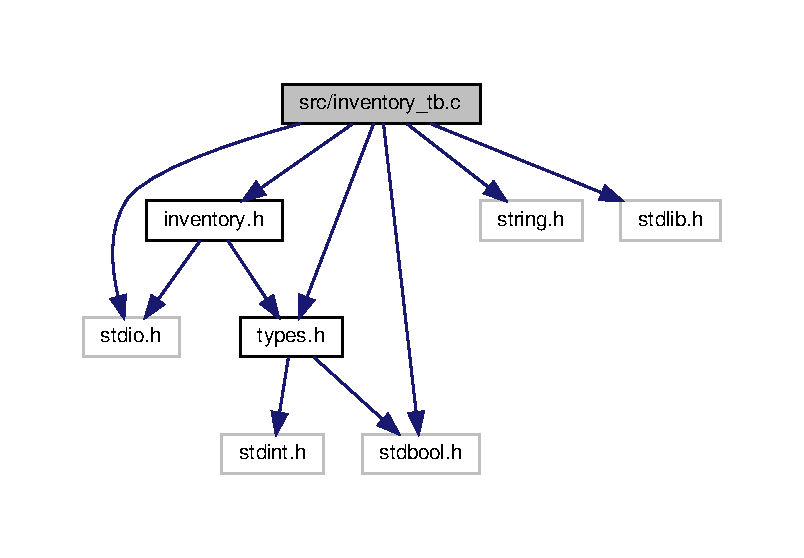
\includegraphics[width=350pt]{inventory__tb_8c__incl}
\end{center}
\end{figure}
\subsection*{Macros}
\begin{DoxyCompactItemize}
\item 
\mbox{\Hypertarget{inventory__tb_8c_aa8de6ad987cfa13b647db341b8dcc510}\label{inventory__tb_8c_aa8de6ad987cfa13b647db341b8dcc510}} 
\#define {\bfseries \+\_\+\+T\+E\+S\+T\+\_\+H}
\item 
\mbox{\Hypertarget{inventory__tb_8c_a66290957baed5df3930ada4cb8caccf1}\label{inventory__tb_8c_a66290957baed5df3930ada4cb8caccf1}} 
\#define {\bfseries K\+R\+ED}~\char`\"{}\textbackslash{}x1B\mbox{[}31m\char`\"{}
\item 
\mbox{\Hypertarget{inventory__tb_8c_ac081c83b067273757f7a2e54a5957d41}\label{inventory__tb_8c_ac081c83b067273757f7a2e54a5957d41}} 
\#define {\bfseries K\+G\+RN}~\char`\"{}\textbackslash{}x1B\mbox{[}32m\char`\"{}
\item 
\mbox{\Hypertarget{inventory__tb_8c_a897b10d246533c95ba86cb79f92e465a}\label{inventory__tb_8c_a897b10d246533c95ba86cb79f92e465a}} 
\#define {\bfseries K\+Y\+EL}~\char`\"{}\textbackslash{}x1B\mbox{[}33m\char`\"{}
\item 
\mbox{\Hypertarget{inventory__tb_8c_a32036c94dbb166a3f874b7efc169841f}\label{inventory__tb_8c_a32036c94dbb166a3f874b7efc169841f}} 
\#define {\bfseries K\+C\+YN}~\char`\"{}\textbackslash{}x1B\mbox{[}36m\char`\"{}
\item 
\mbox{\Hypertarget{inventory__tb_8c_ab702106cf3b3e96750b6845ded4e0299}\label{inventory__tb_8c_ab702106cf3b3e96750b6845ded4e0299}} 
\#define {\bfseries R\+E\+S\+ET}~\char`\"{}\textbackslash{}033\mbox{[}0m\char`\"{}
\item 
\#define {\bfseries P\+R\+I\+N\+T\+\_\+\+T\+E\+S\+T\+\_\+\+R\+E\+S\+U\+LT}(x)
\item 
\mbox{\Hypertarget{inventory__tb_8c_a4a5b9a0026e80b1cfbfbbc3fa700ed31}\label{inventory__tb_8c_a4a5b9a0026e80b1cfbfbbc3fa700ed31}} 
\#define {\bfseries P\+R\+I\+N\+T\+\_\+\+P\+A\+S\+S\+E\+D\+\_\+\+P\+E\+R\+C\+E\+N\+T\+A\+GE}~printf(\char`\"{}Tests passed \%d\%\%\textbackslash{}n\char`\"{}, ((\+\_\+\+\_\+test\+\_\+passed $\ast$ 100) / \+\_\+\+\_\+test\+\_\+counter))
\item 
\mbox{\Hypertarget{inventory__tb_8c_a2a77d2f2c5b698c69c19e1f8782bf709}\label{inventory__tb_8c_a2a77d2f2c5b698c69c19e1f8782bf709}} 
\#define {\bfseries M\+A\+X\+\_\+\+T\+E\+S\+TS}~17
\end{DoxyCompactItemize}
\subsection*{Functions}
\begin{DoxyCompactItemize}
\item 
void \hyperlink{inventory__tb_8c_a33638f1a88ae16ab8d6bee00145b82b8}{test1\+\_\+inventory\+\_\+create} ()
\item 
void \hyperlink{inventory__tb_8c_a73a6080c360a8870c4ffc734e989c8b3}{test2\+\_\+inventory\+\_\+create} ()
\item 
void \hyperlink{inventory__tb_8c_a40a21fc4411716ecfa2bbb33c783df94}{test1\+\_\+inventory\+\_\+add\+\_\+id} ()
\item 
void \hyperlink{inventory__tb_8c_abfb3407529398f76999549e42d567a7e}{test2\+\_\+inventory\+\_\+add\+\_\+id} ()
\item 
void \hyperlink{inventory__tb_8c_a155511682587d9cd63fbd2b62c74dffe}{test1\+\_\+inventory\+\_\+del\+\_\+id} ()
\item 
void \hyperlink{inventory__tb_8c_a52850510d17b4f1c105123fdd9e93906}{test2\+\_\+inventory\+\_\+del\+\_\+id} ()
\item 
void \hyperlink{inventory__tb_8c_a596b3986287f989bbbcaaad879c0c516}{test1\+\_\+inventory\+\_\+has\+\_\+id} ()
\item 
void \hyperlink{inventory__tb_8c_a3a90d9e6b5fb0cabdb8608919256805e}{test2\+\_\+inventory\+\_\+has\+\_\+id} ()
\item 
void \hyperlink{inventory__tb_8c_a17c03f02b989bb00b04155c12fe2af9d}{test1\+\_\+inventory\+\_\+get\+\_\+max} ()
\item 
void \hyperlink{inventory__tb_8c_abddcab377edb21235d6746668597fde2}{test2\+\_\+inventory\+\_\+get\+\_\+max} ()
\item 
void \hyperlink{inventory__tb_8c_a785aa6d245c8e804d5de1e32987ddf8d}{test1\+\_\+inventory\+\_\+get\+\_\+total} ()
\item 
void \hyperlink{inventory__tb_8c_aeec52e4144e58ca0d4c45e877082122f}{test2\+\_\+inventory\+\_\+get\+\_\+total} ()
\item 
void \hyperlink{inventory__tb_8c_a7eb3ba387e33c42ff45331c9d9aada34}{test1\+\_\+inventory\+\_\+is\+\_\+full} ()
\item 
void \hyperlink{inventory__tb_8c_a1c9e567d4919d5aaccc9580815a8a81d}{test2\+\_\+inventory\+\_\+is\+\_\+full} ()
\item 
void \hyperlink{inventory__tb_8c_afe8c9730e30b58535afc0481970ab2b1}{test1\+\_\+inventory\+\_\+is\+\_\+empty} ()
\item 
void \hyperlink{inventory__tb_8c_a4d2a2a4d4ba59446d013debfe9bf05dc}{test2\+\_\+inventory\+\_\+is\+\_\+empty} ()
\item 
int \hyperlink{inventory__tb_8c_a3c04138a5bfe5d72780bb7e82a18e627}{main} (int argc, char $\ast$$\ast$argv)
\begin{DoxyCompactList}\small\item\em Funcion principal de pruebas para el modulo Inventory. \end{DoxyCompactList}\end{DoxyCompactItemize}


\subsection{Detailed Description}
Main for test the inventory. 

\begin{DoxyAuthor}{Author}
Gonzalo Serrano 
\end{DoxyAuthor}
\begin{DoxyVersion}{Version}
1.\+0 
\end{DoxyVersion}
\begin{DoxyDate}{Date}
18/03/2019 
\end{DoxyDate}


\subsection{Macro Definition Documentation}
\mbox{\Hypertarget{inventory__tb_8c_a6c00863b1d44e38839b1f4b49d04f403}\label{inventory__tb_8c_a6c00863b1d44e38839b1f4b49d04f403}} 
\index{inventory\+\_\+tb.\+c@{inventory\+\_\+tb.\+c}!P\+R\+I\+N\+T\+\_\+\+T\+E\+S\+T\+\_\+\+R\+E\+S\+U\+LT@{P\+R\+I\+N\+T\+\_\+\+T\+E\+S\+T\+\_\+\+R\+E\+S\+U\+LT}}
\index{P\+R\+I\+N\+T\+\_\+\+T\+E\+S\+T\+\_\+\+R\+E\+S\+U\+LT@{P\+R\+I\+N\+T\+\_\+\+T\+E\+S\+T\+\_\+\+R\+E\+S\+U\+LT}!inventory\+\_\+tb.\+c@{inventory\+\_\+tb.\+c}}
\subsubsection{\texorpdfstring{P\+R\+I\+N\+T\+\_\+\+T\+E\+S\+T\+\_\+\+R\+E\+S\+U\+LT}{PRINT\_TEST\_RESULT}}
{\footnotesize\ttfamily \#define P\+R\+I\+N\+T\+\_\+\+T\+E\+S\+T\+\_\+\+R\+E\+S\+U\+LT(\begin{DoxyParamCaption}\item[{}]{x }\end{DoxyParamCaption})}

{\bfseries Value\+:}
\begin{DoxyCode}
\textcolor{keywordflow}{do}\{\(\backslash\)
    \_\_test\_counter++; \(\backslash\)
    \_\_pass = (x); \(\backslash\)
    \_\_test\_passed = (\_\_pass)? \_\_test\_passed + 1 : \_\_test\_passed;\(\backslash\)
    printf(KYEL \textcolor{stringliteral}{"%s"} RESET \textcolor{stringliteral}{" line "}  \textcolor{stringliteral}{"%d "} KCYN \textcolor{stringliteral}{"%s"} RESET \textcolor{stringliteral}{": %s\(\backslash\)n"}, \(\backslash\)
     \_\_FILE\_\_, \_\_LINE\_\_ , \_\_FUNCTION\_\_, \(\backslash\)
     ((!\_\_pass) ? KRED \textcolor{stringliteral}{"NOT PASS"} RESET : KGRN \textcolor{stringliteral}{"PASS"} RESET));  \(\backslash\)
  \} \textcolor{keywordflow}{while} (0)
\end{DoxyCode}


\subsection{Function Documentation}
\mbox{\Hypertarget{inventory__tb_8c_a33638f1a88ae16ab8d6bee00145b82b8}\label{inventory__tb_8c_a33638f1a88ae16ab8d6bee00145b82b8}} 
\index{inventory\+\_\+tb.\+c@{inventory\+\_\+tb.\+c}!test1\+\_\+inventory\+\_\+create@{test1\+\_\+inventory\+\_\+create}}
\index{test1\+\_\+inventory\+\_\+create@{test1\+\_\+inventory\+\_\+create}!inventory\+\_\+tb.\+c@{inventory\+\_\+tb.\+c}}
\subsubsection{\texorpdfstring{test1\+\_\+inventory\+\_\+create()}{test1\_inventory\_create()}}
{\footnotesize\ttfamily void test1\+\_\+inventory\+\_\+create (\begin{DoxyParamCaption}{ }\end{DoxyParamCaption})}

\begin{DoxyRefDesc}{Test}
\item[\hyperlink{test__test000001}{Test}]Creates an inventory on an integer \end{DoxyRefDesc}
\begin{DoxyPrecond}{Precondition}
inventory set on an integer 
\end{DoxyPrecond}
\begin{DoxyPostcond}{Postcondition}
A null pointer to the created inventory 
\end{DoxyPostcond}
\mbox{\Hypertarget{inventory__tb_8c_a73a6080c360a8870c4ffc734e989c8b3}\label{inventory__tb_8c_a73a6080c360a8870c4ffc734e989c8b3}} 
\index{inventory\+\_\+tb.\+c@{inventory\+\_\+tb.\+c}!test2\+\_\+inventory\+\_\+create@{test2\+\_\+inventory\+\_\+create}}
\index{test2\+\_\+inventory\+\_\+create@{test2\+\_\+inventory\+\_\+create}!inventory\+\_\+tb.\+c@{inventory\+\_\+tb.\+c}}
\subsubsection{\texorpdfstring{test2\+\_\+inventory\+\_\+create()}{test2\_inventory\_create()}}
{\footnotesize\ttfamily void test2\+\_\+inventory\+\_\+create (\begin{DoxyParamCaption}{ }\end{DoxyParamCaption})}

\begin{DoxyRefDesc}{Test}
\item[\hyperlink{test__test000002}{Test}]Creates an inventory on an inventory \end{DoxyRefDesc}
\begin{DoxyPrecond}{Precondition}
The integer set on an inventory 
\end{DoxyPrecond}
\begin{DoxyPostcond}{Postcondition}
A pointer to the created inventory 
\end{DoxyPostcond}
\mbox{\Hypertarget{inventory__tb_8c_a40a21fc4411716ecfa2bbb33c783df94}\label{inventory__tb_8c_a40a21fc4411716ecfa2bbb33c783df94}} 
\index{inventory\+\_\+tb.\+c@{inventory\+\_\+tb.\+c}!test1\+\_\+inventory\+\_\+add\+\_\+id@{test1\+\_\+inventory\+\_\+add\+\_\+id}}
\index{test1\+\_\+inventory\+\_\+add\+\_\+id@{test1\+\_\+inventory\+\_\+add\+\_\+id}!inventory\+\_\+tb.\+c@{inventory\+\_\+tb.\+c}}
\subsubsection{\texorpdfstring{test1\+\_\+inventory\+\_\+add\+\_\+id()}{test1\_inventory\_add\_id()}}
{\footnotesize\ttfamily void test1\+\_\+inventory\+\_\+add\+\_\+id (\begin{DoxyParamCaption}{ }\end{DoxyParamCaption})}

\begin{DoxyRefDesc}{Test}
\item[\hyperlink{test__test000003}{Test}]Add an id to the inventory \end{DoxyRefDesc}
\begin{DoxyPrecond}{Precondition}
The integer N\+O\+\_\+\+ID as parameter 
\end{DoxyPrecond}
\begin{DoxyPostcond}{Postcondition}
An E\+R\+R\+OR to the introduced id 
\end{DoxyPostcond}
\mbox{\Hypertarget{inventory__tb_8c_abfb3407529398f76999549e42d567a7e}\label{inventory__tb_8c_abfb3407529398f76999549e42d567a7e}} 
\index{inventory\+\_\+tb.\+c@{inventory\+\_\+tb.\+c}!test2\+\_\+inventory\+\_\+add\+\_\+id@{test2\+\_\+inventory\+\_\+add\+\_\+id}}
\index{test2\+\_\+inventory\+\_\+add\+\_\+id@{test2\+\_\+inventory\+\_\+add\+\_\+id}!inventory\+\_\+tb.\+c@{inventory\+\_\+tb.\+c}}
\subsubsection{\texorpdfstring{test2\+\_\+inventory\+\_\+add\+\_\+id()}{test2\_inventory\_add\_id()}}
{\footnotesize\ttfamily void test2\+\_\+inventory\+\_\+add\+\_\+id (\begin{DoxyParamCaption}{ }\end{DoxyParamCaption})}

\begin{DoxyRefDesc}{Test}
\item[\hyperlink{test__test000004}{Test}]Add an id to the inventory \end{DoxyRefDesc}
\begin{DoxyPrecond}{Precondition}
The integer 1 as parameter 
\end{DoxyPrecond}
\begin{DoxyPostcond}{Postcondition}
An OK to the introduced id 
\end{DoxyPostcond}
\mbox{\Hypertarget{inventory__tb_8c_a155511682587d9cd63fbd2b62c74dffe}\label{inventory__tb_8c_a155511682587d9cd63fbd2b62c74dffe}} 
\index{inventory\+\_\+tb.\+c@{inventory\+\_\+tb.\+c}!test1\+\_\+inventory\+\_\+del\+\_\+id@{test1\+\_\+inventory\+\_\+del\+\_\+id}}
\index{test1\+\_\+inventory\+\_\+del\+\_\+id@{test1\+\_\+inventory\+\_\+del\+\_\+id}!inventory\+\_\+tb.\+c@{inventory\+\_\+tb.\+c}}
\subsubsection{\texorpdfstring{test1\+\_\+inventory\+\_\+del\+\_\+id()}{test1\_inventory\_del\_id()}}
{\footnotesize\ttfamily void test1\+\_\+inventory\+\_\+del\+\_\+id (\begin{DoxyParamCaption}{ }\end{DoxyParamCaption})}

\begin{DoxyRefDesc}{Test}
\item[\hyperlink{test__test000005}{Test}]Deletes an id to the inventory \end{DoxyRefDesc}
\begin{DoxyPrecond}{Precondition}
The integer 2 as parameter 
\end{DoxyPrecond}
\begin{DoxyPostcond}{Postcondition}
An E\+R\+R\+OR to the introduced id 
\end{DoxyPostcond}
\mbox{\Hypertarget{inventory__tb_8c_a52850510d17b4f1c105123fdd9e93906}\label{inventory__tb_8c_a52850510d17b4f1c105123fdd9e93906}} 
\index{inventory\+\_\+tb.\+c@{inventory\+\_\+tb.\+c}!test2\+\_\+inventory\+\_\+del\+\_\+id@{test2\+\_\+inventory\+\_\+del\+\_\+id}}
\index{test2\+\_\+inventory\+\_\+del\+\_\+id@{test2\+\_\+inventory\+\_\+del\+\_\+id}!inventory\+\_\+tb.\+c@{inventory\+\_\+tb.\+c}}
\subsubsection{\texorpdfstring{test2\+\_\+inventory\+\_\+del\+\_\+id()}{test2\_inventory\_del\_id()}}
{\footnotesize\ttfamily void test2\+\_\+inventory\+\_\+del\+\_\+id (\begin{DoxyParamCaption}{ }\end{DoxyParamCaption})}

\begin{DoxyRefDesc}{Test}
\item[\hyperlink{test__test000006}{Test}]Deletes an id to the inventory \end{DoxyRefDesc}
\begin{DoxyPrecond}{Precondition}
The integer 1 as parameter 
\end{DoxyPrecond}
\begin{DoxyPostcond}{Postcondition}
An OK to the introduced id 
\end{DoxyPostcond}
\mbox{\Hypertarget{inventory__tb_8c_a596b3986287f989bbbcaaad879c0c516}\label{inventory__tb_8c_a596b3986287f989bbbcaaad879c0c516}} 
\index{inventory\+\_\+tb.\+c@{inventory\+\_\+tb.\+c}!test1\+\_\+inventory\+\_\+has\+\_\+id@{test1\+\_\+inventory\+\_\+has\+\_\+id}}
\index{test1\+\_\+inventory\+\_\+has\+\_\+id@{test1\+\_\+inventory\+\_\+has\+\_\+id}!inventory\+\_\+tb.\+c@{inventory\+\_\+tb.\+c}}
\subsubsection{\texorpdfstring{test1\+\_\+inventory\+\_\+has\+\_\+id()}{test1\_inventory\_has\_id()}}
{\footnotesize\ttfamily void test1\+\_\+inventory\+\_\+has\+\_\+id (\begin{DoxyParamCaption}{ }\end{DoxyParamCaption})}

\begin{DoxyRefDesc}{Test}
\item[\hyperlink{test__test000007}{Test}]Find if the inventory has that id \end{DoxyRefDesc}
\begin{DoxyPrecond}{Precondition}
The integer 2 as parameter 
\end{DoxyPrecond}
\begin{DoxyPostcond}{Postcondition}
An E\+R\+R\+OR to the introduced id 
\end{DoxyPostcond}
\mbox{\Hypertarget{inventory__tb_8c_a3a90d9e6b5fb0cabdb8608919256805e}\label{inventory__tb_8c_a3a90d9e6b5fb0cabdb8608919256805e}} 
\index{inventory\+\_\+tb.\+c@{inventory\+\_\+tb.\+c}!test2\+\_\+inventory\+\_\+has\+\_\+id@{test2\+\_\+inventory\+\_\+has\+\_\+id}}
\index{test2\+\_\+inventory\+\_\+has\+\_\+id@{test2\+\_\+inventory\+\_\+has\+\_\+id}!inventory\+\_\+tb.\+c@{inventory\+\_\+tb.\+c}}
\subsubsection{\texorpdfstring{test2\+\_\+inventory\+\_\+has\+\_\+id()}{test2\_inventory\_has\_id()}}
{\footnotesize\ttfamily void test2\+\_\+inventory\+\_\+has\+\_\+id (\begin{DoxyParamCaption}{ }\end{DoxyParamCaption})}

\begin{DoxyRefDesc}{Test}
\item[\hyperlink{test__test000008}{Test}]Creates a space on an integer \end{DoxyRefDesc}
\begin{DoxyPrecond}{Precondition}
The integer 1 as parameter 
\end{DoxyPrecond}
\begin{DoxyPostcond}{Postcondition}
An OK to the introduced id 
\end{DoxyPostcond}
\mbox{\Hypertarget{inventory__tb_8c_a17c03f02b989bb00b04155c12fe2af9d}\label{inventory__tb_8c_a17c03f02b989bb00b04155c12fe2af9d}} 
\index{inventory\+\_\+tb.\+c@{inventory\+\_\+tb.\+c}!test1\+\_\+inventory\+\_\+get\+\_\+max@{test1\+\_\+inventory\+\_\+get\+\_\+max}}
\index{test1\+\_\+inventory\+\_\+get\+\_\+max@{test1\+\_\+inventory\+\_\+get\+\_\+max}!inventory\+\_\+tb.\+c@{inventory\+\_\+tb.\+c}}
\subsubsection{\texorpdfstring{test1\+\_\+inventory\+\_\+get\+\_\+max()}{test1\_inventory\_get\_max()}}
{\footnotesize\ttfamily void test1\+\_\+inventory\+\_\+get\+\_\+max (\begin{DoxyParamCaption}{ }\end{DoxyParamCaption})}

\begin{DoxyRefDesc}{Test}
\item[\hyperlink{test__test000009}{Test}]Get the maximun cunatity of objects in the inventory \end{DoxyRefDesc}
\begin{DoxyPrecond}{Precondition}
The inventory is initialised and and integer id 1 is added 
\end{DoxyPrecond}
\begin{DoxyPostcond}{Postcondition}
An OK to the introduced id 
\end{DoxyPostcond}
\mbox{\Hypertarget{inventory__tb_8c_abddcab377edb21235d6746668597fde2}\label{inventory__tb_8c_abddcab377edb21235d6746668597fde2}} 
\index{inventory\+\_\+tb.\+c@{inventory\+\_\+tb.\+c}!test2\+\_\+inventory\+\_\+get\+\_\+max@{test2\+\_\+inventory\+\_\+get\+\_\+max}}
\index{test2\+\_\+inventory\+\_\+get\+\_\+max@{test2\+\_\+inventory\+\_\+get\+\_\+max}!inventory\+\_\+tb.\+c@{inventory\+\_\+tb.\+c}}
\subsubsection{\texorpdfstring{test2\+\_\+inventory\+\_\+get\+\_\+max()}{test2\_inventory\_get\_max()}}
{\footnotesize\ttfamily void test2\+\_\+inventory\+\_\+get\+\_\+max (\begin{DoxyParamCaption}{ }\end{DoxyParamCaption})}

\begin{DoxyRefDesc}{Test}
\item[\hyperlink{test__test000010}{Test}]Get the maximun cunatity of objects in the inventory \end{DoxyRefDesc}
\begin{DoxyPrecond}{Precondition}
The inventory is uninitialised 
\end{DoxyPrecond}
\begin{DoxyPostcond}{Postcondition}
An E\+R\+R\+OR 
\end{DoxyPostcond}
\mbox{\Hypertarget{inventory__tb_8c_a785aa6d245c8e804d5de1e32987ddf8d}\label{inventory__tb_8c_a785aa6d245c8e804d5de1e32987ddf8d}} 
\index{inventory\+\_\+tb.\+c@{inventory\+\_\+tb.\+c}!test1\+\_\+inventory\+\_\+get\+\_\+total@{test1\+\_\+inventory\+\_\+get\+\_\+total}}
\index{test1\+\_\+inventory\+\_\+get\+\_\+total@{test1\+\_\+inventory\+\_\+get\+\_\+total}!inventory\+\_\+tb.\+c@{inventory\+\_\+tb.\+c}}
\subsubsection{\texorpdfstring{test1\+\_\+inventory\+\_\+get\+\_\+total()}{test1\_inventory\_get\_total()}}
{\footnotesize\ttfamily void test1\+\_\+inventory\+\_\+get\+\_\+total (\begin{DoxyParamCaption}{ }\end{DoxyParamCaption})}

\begin{DoxyRefDesc}{Test}
\item[\hyperlink{test__test000011}{Test}]Get the total of objects stored on the inventory \end{DoxyRefDesc}
\begin{DoxyPrecond}{Precondition}
The inventory initialised 
\end{DoxyPrecond}
\begin{DoxyPostcond}{Postcondition}
An OK to the introduced inventory 
\end{DoxyPostcond}
\mbox{\Hypertarget{inventory__tb_8c_aeec52e4144e58ca0d4c45e877082122f}\label{inventory__tb_8c_aeec52e4144e58ca0d4c45e877082122f}} 
\index{inventory\+\_\+tb.\+c@{inventory\+\_\+tb.\+c}!test2\+\_\+inventory\+\_\+get\+\_\+total@{test2\+\_\+inventory\+\_\+get\+\_\+total}}
\index{test2\+\_\+inventory\+\_\+get\+\_\+total@{test2\+\_\+inventory\+\_\+get\+\_\+total}!inventory\+\_\+tb.\+c@{inventory\+\_\+tb.\+c}}
\subsubsection{\texorpdfstring{test2\+\_\+inventory\+\_\+get\+\_\+total()}{test2\_inventory\_get\_total()}}
{\footnotesize\ttfamily void test2\+\_\+inventory\+\_\+get\+\_\+total (\begin{DoxyParamCaption}{ }\end{DoxyParamCaption})}

\begin{DoxyRefDesc}{Test}
\item[\hyperlink{test__test000012}{Test}]Get a invalid total of objects stored on the inventory \end{DoxyRefDesc}
\begin{DoxyPrecond}{Precondition}
The inventory uninitialised 
\end{DoxyPrecond}
\begin{DoxyPostcond}{Postcondition}
An E\+R\+R\+OR to the introduced inventory 
\end{DoxyPostcond}
\mbox{\Hypertarget{inventory__tb_8c_a7eb3ba387e33c42ff45331c9d9aada34}\label{inventory__tb_8c_a7eb3ba387e33c42ff45331c9d9aada34}} 
\index{inventory\+\_\+tb.\+c@{inventory\+\_\+tb.\+c}!test1\+\_\+inventory\+\_\+is\+\_\+full@{test1\+\_\+inventory\+\_\+is\+\_\+full}}
\index{test1\+\_\+inventory\+\_\+is\+\_\+full@{test1\+\_\+inventory\+\_\+is\+\_\+full}!inventory\+\_\+tb.\+c@{inventory\+\_\+tb.\+c}}
\subsubsection{\texorpdfstring{test1\+\_\+inventory\+\_\+is\+\_\+full()}{test1\_inventory\_is\_full()}}
{\footnotesize\ttfamily void test1\+\_\+inventory\+\_\+is\+\_\+full (\begin{DoxyParamCaption}{ }\end{DoxyParamCaption})}

\begin{DoxyRefDesc}{Test}
\item[\hyperlink{test__test000013}{Test}]Shows if the inventory is full \end{DoxyRefDesc}
\begin{DoxyPrecond}{Precondition}
The integer 1 as parameter 
\end{DoxyPrecond}
\begin{DoxyPostcond}{Postcondition}
An E\+R\+R\+OR to the introduced inventory 
\end{DoxyPostcond}
\mbox{\Hypertarget{inventory__tb_8c_a1c9e567d4919d5aaccc9580815a8a81d}\label{inventory__tb_8c_a1c9e567d4919d5aaccc9580815a8a81d}} 
\index{inventory\+\_\+tb.\+c@{inventory\+\_\+tb.\+c}!test2\+\_\+inventory\+\_\+is\+\_\+full@{test2\+\_\+inventory\+\_\+is\+\_\+full}}
\index{test2\+\_\+inventory\+\_\+is\+\_\+full@{test2\+\_\+inventory\+\_\+is\+\_\+full}!inventory\+\_\+tb.\+c@{inventory\+\_\+tb.\+c}}
\subsubsection{\texorpdfstring{test2\+\_\+inventory\+\_\+is\+\_\+full()}{test2\_inventory\_is\_full()}}
{\footnotesize\ttfamily void test2\+\_\+inventory\+\_\+is\+\_\+full (\begin{DoxyParamCaption}{ }\end{DoxyParamCaption})}

\begin{DoxyRefDesc}{Test}
\item[\hyperlink{test__test000014}{Test}]Shows if the inventory is full \end{DoxyRefDesc}
\begin{DoxyPrecond}{Precondition}
The integer 1 to 6 as parameter 
\end{DoxyPrecond}
\begin{DoxyPostcond}{Postcondition}
A OK to the introduced inventory 
\end{DoxyPostcond}
\mbox{\Hypertarget{inventory__tb_8c_afe8c9730e30b58535afc0481970ab2b1}\label{inventory__tb_8c_afe8c9730e30b58535afc0481970ab2b1}} 
\index{inventory\+\_\+tb.\+c@{inventory\+\_\+tb.\+c}!test1\+\_\+inventory\+\_\+is\+\_\+empty@{test1\+\_\+inventory\+\_\+is\+\_\+empty}}
\index{test1\+\_\+inventory\+\_\+is\+\_\+empty@{test1\+\_\+inventory\+\_\+is\+\_\+empty}!inventory\+\_\+tb.\+c@{inventory\+\_\+tb.\+c}}
\subsubsection{\texorpdfstring{test1\+\_\+inventory\+\_\+is\+\_\+empty()}{test1\_inventory\_is\_empty()}}
{\footnotesize\ttfamily void test1\+\_\+inventory\+\_\+is\+\_\+empty (\begin{DoxyParamCaption}{ }\end{DoxyParamCaption})}

\begin{DoxyRefDesc}{Test}
\item[\hyperlink{test__test000015}{Test}]Shows if the inventory is empty without one obj in it \end{DoxyRefDesc}
\begin{DoxyPrecond}{Precondition}
inventory as parameter 
\end{DoxyPrecond}
\begin{DoxyPostcond}{Postcondition}
An E\+R\+R\+OR to the introduced inventory 
\end{DoxyPostcond}
\mbox{\Hypertarget{inventory__tb_8c_a4d2a2a4d4ba59446d013debfe9bf05dc}\label{inventory__tb_8c_a4d2a2a4d4ba59446d013debfe9bf05dc}} 
\index{inventory\+\_\+tb.\+c@{inventory\+\_\+tb.\+c}!test2\+\_\+inventory\+\_\+is\+\_\+empty@{test2\+\_\+inventory\+\_\+is\+\_\+empty}}
\index{test2\+\_\+inventory\+\_\+is\+\_\+empty@{test2\+\_\+inventory\+\_\+is\+\_\+empty}!inventory\+\_\+tb.\+c@{inventory\+\_\+tb.\+c}}
\subsubsection{\texorpdfstring{test2\+\_\+inventory\+\_\+is\+\_\+empty()}{test2\_inventory\_is\_empty()}}
{\footnotesize\ttfamily void test2\+\_\+inventory\+\_\+is\+\_\+empty (\begin{DoxyParamCaption}{ }\end{DoxyParamCaption})}

\begin{DoxyRefDesc}{Test}
\item[\hyperlink{test__test000016}{Test}]Shows if the inventory is empty without any obj in it \end{DoxyRefDesc}
\begin{DoxyPrecond}{Precondition}
inventory as parameter 
\end{DoxyPrecond}
\begin{DoxyPostcond}{Postcondition}
A OK to the introduced inventory 
\end{DoxyPostcond}
\mbox{\Hypertarget{inventory__tb_8c_a3c04138a5bfe5d72780bb7e82a18e627}\label{inventory__tb_8c_a3c04138a5bfe5d72780bb7e82a18e627}} 
\index{inventory\+\_\+tb.\+c@{inventory\+\_\+tb.\+c}!main@{main}}
\index{main@{main}!inventory\+\_\+tb.\+c@{inventory\+\_\+tb.\+c}}
\subsubsection{\texorpdfstring{main()}{main()}}
{\footnotesize\ttfamily int main (\begin{DoxyParamCaption}\item[{int}]{argc,  }\item[{char $\ast$$\ast$}]{argv }\end{DoxyParamCaption})}



Funcion principal de pruebas para el modulo Inventory. 

Dos modos de ejecucion\+: 1.-\/\+Si se ejecuta sin parametros se ejecutan todas las pruebas 2.-\/\+Si se ejecuta con un numero entre 1 y el numero de pruebas solo ejecuta la prueba indicada 
\hypertarget{link_8c}{}\section{src/link.c File Reference}
\label{link_8c}\index{src/link.\+c@{src/link.\+c}}


link functions  


{\ttfamily \#include \char`\"{}link.\+h\char`\"{}}\newline
{\ttfamily \#include $<$stdio.\+h$>$}\newline
{\ttfamily \#include $<$stdlib.\+h$>$}\newline
{\ttfamily \#include $<$string.\+h$>$}\newline
Include dependency graph for link.\+c\+:
\nopagebreak
\begin{figure}[H]
\begin{center}
\leavevmode
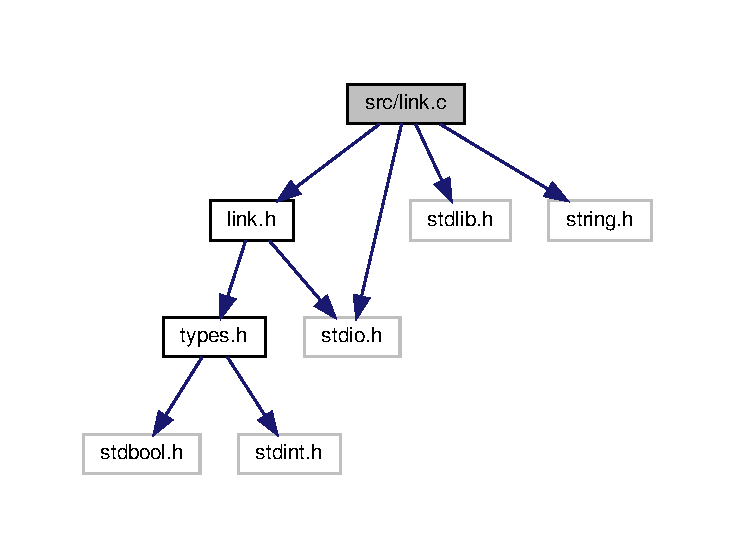
\includegraphics[width=350pt]{link_8c__incl}
\end{center}
\end{figure}
\subsection*{Data Structures}
\begin{DoxyCompactItemize}
\item 
struct \hyperlink{struct__Link}{\+\_\+\+Link}
\end{DoxyCompactItemize}
\subsection*{Functions}
\begin{DoxyCompactItemize}
\item 
\hyperlink{struct__Link}{Link} $\ast$ \hyperlink{link_8c_aaf21d03943afcbed370ca720f972482c}{link\+\_\+create} ()
\begin{DoxyCompactList}\small\item\em initializes a new link \end{DoxyCompactList}\item 
\hyperlink{types_8h_a32c27cc471df37f4fc818d65de0a56c4}{S\+T\+A\+T\+US} \hyperlink{link_8c_a85c4dd77887bf31f651ea1162144d712}{link\+\_\+destroy} (\hyperlink{struct__Link}{Link} $\ast$link)
\begin{DoxyCompactList}\small\item\em destroys a link \end{DoxyCompactList}\item 
\hyperlink{types_8h_a845e604fb28f7e3d97549da3448149d3}{Id} \hyperlink{link_8c_a2bbd320f995a72b2ea7ea639b1c81892}{link\+\_\+get\+\_\+id} (\hyperlink{struct__Link}{Link} $\ast$link)
\begin{DoxyCompactList}\small\item\em Gets the id of a link. \end{DoxyCompactList}\item 
\hyperlink{types_8h_a845e604fb28f7e3d97549da3448149d3}{Id} \hyperlink{link_8c_a6e03d80f1a54c61a366a4a81aaca8106}{link\+\_\+get\+\_\+from} (\hyperlink{struct__Link}{Link} $\ast$link)
\begin{DoxyCompactList}\small\item\em Gets the destination id of a link. \end{DoxyCompactList}\item 
\hyperlink{types_8h_a845e604fb28f7e3d97549da3448149d3}{Id} \hyperlink{link_8c_a74cf03260545d4b8d19228aab08bdffd}{link\+\_\+get\+\_\+to} (\hyperlink{struct__Link}{Link} $\ast$link)
\begin{DoxyCompactList}\small\item\em gets the id\+To of a link \end{DoxyCompactList}\item 
const char $\ast$ \hyperlink{link_8c_aaab4c9c7d5492873cafd9e11dc0f8059}{link\+\_\+get\+\_\+name} (\hyperlink{struct__Link}{Link} $\ast$link)
\begin{DoxyCompactList}\small\item\em gets the name of a link \end{DoxyCompactList}\item 
\hyperlink{link_8h_ab0033b911037fd995258d117e65461e0}{Link\+State} \hyperlink{link_8c_acbc8c044a54ceb16e24d828370d98244}{link\+\_\+get\+\_\+state} (\hyperlink{struct__Link}{Link} $\ast$link)
\begin{DoxyCompactList}\small\item\em gets the state of a link O\+P\+EN or C\+L\+O\+SE \end{DoxyCompactList}\item 
\hyperlink{types_8h_a32c27cc471df37f4fc818d65de0a56c4}{S\+T\+A\+T\+US} \hyperlink{link_8c_a7e39694824973f396f87d8c01e9b824a}{link\+\_\+set\+\_\+state} (\hyperlink{struct__Link}{Link} $\ast$link, \hyperlink{link_8h_ab0033b911037fd995258d117e65461e0}{Link\+State} state)
\begin{DoxyCompactList}\small\item\em Sets the state of a given link. \end{DoxyCompactList}\item 
\hyperlink{types_8h_a32c27cc471df37f4fc818d65de0a56c4}{S\+T\+A\+T\+US} \hyperlink{link_8c_a3fd49fb1a3f19be4fc800ff07820cafb}{link\+\_\+set\+\_\+id} (\hyperlink{struct__Link}{Link} $\ast$link, \hyperlink{types_8h_a845e604fb28f7e3d97549da3448149d3}{Id} id)
\begin{DoxyCompactList}\small\item\em it set the id of a link on the structure \end{DoxyCompactList}\item 
\hyperlink{types_8h_a32c27cc471df37f4fc818d65de0a56c4}{S\+T\+A\+T\+US} \hyperlink{link_8c_aa0baad3998d882d695136d9112485e78}{link\+\_\+set\+\_\+from} (\hyperlink{struct__Link}{Link} $\ast$link, \hyperlink{types_8h_a845e604fb28f7e3d97549da3448149d3}{Id} id)
\begin{DoxyCompactList}\small\item\em it set the id\+From of a link on the structure \end{DoxyCompactList}\item 
\hyperlink{types_8h_a32c27cc471df37f4fc818d65de0a56c4}{S\+T\+A\+T\+US} \hyperlink{link_8c_a48f0e8c3924c608346cef5119a0125a0}{link\+\_\+set\+\_\+to} (\hyperlink{struct__Link}{Link} $\ast$link, \hyperlink{types_8h_a845e604fb28f7e3d97549da3448149d3}{Id} id)
\begin{DoxyCompactList}\small\item\em it set the id\+To of a link on the structure \end{DoxyCompactList}\item 
\hyperlink{types_8h_a32c27cc471df37f4fc818d65de0a56c4}{S\+T\+A\+T\+US} \hyperlink{link_8c_a8cf278a0dc6226ed88166f5278d86ca7}{link\+\_\+set\+\_\+name} (\hyperlink{struct__Link}{Link} $\ast$link, const char $\ast$name)
\begin{DoxyCompactList}\small\item\em it set the id of a link on the structure \end{DoxyCompactList}\item 
\hyperlink{types_8h_a32c27cc471df37f4fc818d65de0a56c4}{S\+T\+A\+T\+US} \hyperlink{link_8c_ae42d5937c06a6efccd72041121658b09}{link\+\_\+print} (F\+I\+LE $\ast$stream, \hyperlink{struct__Link}{Link} $\ast$link)
\begin{DoxyCompactList}\small\item\em prints a link. \end{DoxyCompactList}\end{DoxyCompactItemize}


\subsection{Detailed Description}
link functions 

\begin{DoxyVersion}{Version}
0.\+0.\+3 
\end{DoxyVersion}
\begin{DoxyDate}{Date}
19/03/2019 
\end{DoxyDate}
\begin{DoxyAuthor}{Author}
Gonzalo Serrano 
\end{DoxyAuthor}
\begin{DoxyCopyright}{Copyright}
G\+NU Public License 
\end{DoxyCopyright}


\subsection{Function Documentation}
\mbox{\Hypertarget{link_8c_aaf21d03943afcbed370ca720f972482c}\label{link_8c_aaf21d03943afcbed370ca720f972482c}} 
\index{link.\+c@{link.\+c}!link\+\_\+create@{link\+\_\+create}}
\index{link\+\_\+create@{link\+\_\+create}!link.\+c@{link.\+c}}
\subsubsection{\texorpdfstring{link\+\_\+create()}{link\_create()}}
{\footnotesize\ttfamily \hyperlink{struct__Link}{Link}$\ast$ link\+\_\+create (\begin{DoxyParamCaption}{ }\end{DoxyParamCaption})}



initializes a new link 

\begin{DoxyDate}{Date}
19/03/2019 
\end{DoxyDate}
\begin{DoxyAuthor}{Author}
\+: Gonzalo Serrano
\end{DoxyAuthor}

\begin{DoxyParams}{Parameters}
{\em Id} & of the link \\
\hline
\end{DoxyParams}

\begin{DoxyRetVals}{Return values}
{\em \{\+Link$\ast$\}} & -\/ returns a pointer to the new link \\
\hline
\end{DoxyRetVals}
\mbox{\Hypertarget{link_8c_a85c4dd77887bf31f651ea1162144d712}\label{link_8c_a85c4dd77887bf31f651ea1162144d712}} 
\index{link.\+c@{link.\+c}!link\+\_\+destroy@{link\+\_\+destroy}}
\index{link\+\_\+destroy@{link\+\_\+destroy}!link.\+c@{link.\+c}}
\subsubsection{\texorpdfstring{link\+\_\+destroy()}{link\_destroy()}}
{\footnotesize\ttfamily \hyperlink{types_8h_a32c27cc471df37f4fc818d65de0a56c4}{S\+T\+A\+T\+US} link\+\_\+destroy (\begin{DoxyParamCaption}\item[{\hyperlink{struct__Link}{Link} $\ast$}]{link }\end{DoxyParamCaption})}



destroys a link 

\begin{DoxyDate}{Date}
19/03/2019 
\end{DoxyDate}
\begin{DoxyAuthor}{Author}
Gonzalo Serrano
\end{DoxyAuthor}

\begin{DoxyParams}{Parameters}
{\em \{\+Link$\ast$\}} & link -\/ Link pointer \\
\hline
\end{DoxyParams}

\begin{DoxyRetVals}{Return values}
{\em \{void\}} & -\/ Do not returns nothing \\
\hline
\end{DoxyRetVals}
\mbox{\Hypertarget{link_8c_a2bbd320f995a72b2ea7ea639b1c81892}\label{link_8c_a2bbd320f995a72b2ea7ea639b1c81892}} 
\index{link.\+c@{link.\+c}!link\+\_\+get\+\_\+id@{link\+\_\+get\+\_\+id}}
\index{link\+\_\+get\+\_\+id@{link\+\_\+get\+\_\+id}!link.\+c@{link.\+c}}
\subsubsection{\texorpdfstring{link\+\_\+get\+\_\+id()}{link\_get\_id()}}
{\footnotesize\ttfamily \hyperlink{types_8h_a845e604fb28f7e3d97549da3448149d3}{Id} link\+\_\+get\+\_\+id (\begin{DoxyParamCaption}\item[{\hyperlink{struct__Link}{Link} $\ast$}]{link }\end{DoxyParamCaption})}



Gets the id of a link. 

\begin{DoxyDate}{Date}
19/03/2019 
\end{DoxyDate}
\begin{DoxyAuthor}{Author}
Gonzalo Serrano
\end{DoxyAuthor}

\begin{DoxyParams}{Parameters}
{\em \{\+Link$\ast$\}} & link -\/ Link pointer \\
\hline
\end{DoxyParams}

\begin{DoxyRetVals}{Return values}
{\em \{\+Id\}} & -\/ Returns the id of a link \\
\hline
\end{DoxyRetVals}
\mbox{\Hypertarget{link_8c_a6e03d80f1a54c61a366a4a81aaca8106}\label{link_8c_a6e03d80f1a54c61a366a4a81aaca8106}} 
\index{link.\+c@{link.\+c}!link\+\_\+get\+\_\+from@{link\+\_\+get\+\_\+from}}
\index{link\+\_\+get\+\_\+from@{link\+\_\+get\+\_\+from}!link.\+c@{link.\+c}}
\subsubsection{\texorpdfstring{link\+\_\+get\+\_\+from()}{link\_get\_from()}}
{\footnotesize\ttfamily \hyperlink{types_8h_a845e604fb28f7e3d97549da3448149d3}{Id} link\+\_\+get\+\_\+from (\begin{DoxyParamCaption}\item[{\hyperlink{struct__Link}{Link} $\ast$}]{link }\end{DoxyParamCaption})}



Gets the destination id of a link. 

\begin{DoxyDate}{Date}
19/03/2019 
\end{DoxyDate}
\begin{DoxyAuthor}{Author}
Gonzalo Serrano
\end{DoxyAuthor}

\begin{DoxyParams}{Parameters}
{\em \{\+Link$\ast$\}} & link -\/ Link pointer \\
\hline
\end{DoxyParams}

\begin{DoxyRetVals}{Return values}
{\em \{\+Id\}} & -\/ Returns the id\+From of a link \\
\hline
\end{DoxyRetVals}
\mbox{\Hypertarget{link_8c_a74cf03260545d4b8d19228aab08bdffd}\label{link_8c_a74cf03260545d4b8d19228aab08bdffd}} 
\index{link.\+c@{link.\+c}!link\+\_\+get\+\_\+to@{link\+\_\+get\+\_\+to}}
\index{link\+\_\+get\+\_\+to@{link\+\_\+get\+\_\+to}!link.\+c@{link.\+c}}
\subsubsection{\texorpdfstring{link\+\_\+get\+\_\+to()}{link\_get\_to()}}
{\footnotesize\ttfamily \hyperlink{types_8h_a845e604fb28f7e3d97549da3448149d3}{Id} link\+\_\+get\+\_\+to (\begin{DoxyParamCaption}\item[{\hyperlink{struct__Link}{Link} $\ast$}]{link }\end{DoxyParamCaption})}



gets the id\+To of a link 

\begin{DoxyDate}{Date}
19/03/2019 
\end{DoxyDate}
\begin{DoxyAuthor}{Author}
Gonzalo Serrano
\end{DoxyAuthor}

\begin{DoxyParams}{Parameters}
{\em \{\+Link$\ast$\}} & link -\/ Link pointer \\
\hline
\end{DoxyParams}

\begin{DoxyRetVals}{Return values}
{\em \{\+Id\}} & -\/ Returns the id\+To of a link \\
\hline
\end{DoxyRetVals}
\mbox{\Hypertarget{link_8c_aaab4c9c7d5492873cafd9e11dc0f8059}\label{link_8c_aaab4c9c7d5492873cafd9e11dc0f8059}} 
\index{link.\+c@{link.\+c}!link\+\_\+get\+\_\+name@{link\+\_\+get\+\_\+name}}
\index{link\+\_\+get\+\_\+name@{link\+\_\+get\+\_\+name}!link.\+c@{link.\+c}}
\subsubsection{\texorpdfstring{link\+\_\+get\+\_\+name()}{link\_get\_name()}}
{\footnotesize\ttfamily const char$\ast$ link\+\_\+get\+\_\+name (\begin{DoxyParamCaption}\item[{\hyperlink{struct__Link}{Link} $\ast$}]{link }\end{DoxyParamCaption})}



gets the name of a link 

\begin{DoxyDate}{Date}
19/03/2019 
\end{DoxyDate}
\begin{DoxyAuthor}{Author}
Gonzalo Serrano
\end{DoxyAuthor}

\begin{DoxyParams}{Parameters}
{\em \{\+Link$\ast$\}} & link -\/ Link pointer \\
\hline
\end{DoxyParams}

\begin{DoxyRetVals}{Return values}
{\em \{\+Id\}} & -\/ Returns the name of a link \\
\hline
\end{DoxyRetVals}
\mbox{\Hypertarget{link_8c_acbc8c044a54ceb16e24d828370d98244}\label{link_8c_acbc8c044a54ceb16e24d828370d98244}} 
\index{link.\+c@{link.\+c}!link\+\_\+get\+\_\+state@{link\+\_\+get\+\_\+state}}
\index{link\+\_\+get\+\_\+state@{link\+\_\+get\+\_\+state}!link.\+c@{link.\+c}}
\subsubsection{\texorpdfstring{link\+\_\+get\+\_\+state()}{link\_get\_state()}}
{\footnotesize\ttfamily \hyperlink{link_8h_ab0033b911037fd995258d117e65461e0}{Link\+State} link\+\_\+get\+\_\+state (\begin{DoxyParamCaption}\item[{\hyperlink{struct__Link}{Link} $\ast$}]{link }\end{DoxyParamCaption})}



gets the state of a link O\+P\+EN or C\+L\+O\+SE 

\begin{DoxyDate}{Date}
19/03/2019 
\end{DoxyDate}
\begin{DoxyAuthor}{Author}
Gonzalo Serrano
\end{DoxyAuthor}

\begin{DoxyParams}{Parameters}
{\em \{\+Link$\ast$\}} & link -\/ Link pointer \\
\hline
\end{DoxyParams}

\begin{DoxyRetVals}{Return values}
{\em \{\+Link\+State\}} & -\/ Returns the state of a link \\
\hline
\end{DoxyRetVals}
\mbox{\Hypertarget{link_8c_a7e39694824973f396f87d8c01e9b824a}\label{link_8c_a7e39694824973f396f87d8c01e9b824a}} 
\index{link.\+c@{link.\+c}!link\+\_\+set\+\_\+state@{link\+\_\+set\+\_\+state}}
\index{link\+\_\+set\+\_\+state@{link\+\_\+set\+\_\+state}!link.\+c@{link.\+c}}
\subsubsection{\texorpdfstring{link\+\_\+set\+\_\+state()}{link\_set\_state()}}
{\footnotesize\ttfamily \hyperlink{types_8h_a32c27cc471df37f4fc818d65de0a56c4}{S\+T\+A\+T\+US} link\+\_\+set\+\_\+state (\begin{DoxyParamCaption}\item[{\hyperlink{struct__Link}{Link} $\ast$}]{link,  }\item[{\hyperlink{link_8h_ab0033b911037fd995258d117e65461e0}{Link\+State}}]{state }\end{DoxyParamCaption})}



Sets the state of a given link. 

\begin{DoxyDate}{Date}
19/03/2019 
\end{DoxyDate}
\begin{DoxyAuthor}{Author}
Gonzalo Serrano
\end{DoxyAuthor}

\begin{DoxyParams}{Parameters}
{\em \{\+Link$\ast$\}} & link -\/ Link pointer \\
\hline
{\em \{\+Link\+State\}} & id -\/ New state of the link \\
\hline
\end{DoxyParams}
\begin{DoxyReturn}{Returns}
\{S\+T\+A\+T\+US\} -\/ Returns an status 
\end{DoxyReturn}
\mbox{\Hypertarget{link_8c_a3fd49fb1a3f19be4fc800ff07820cafb}\label{link_8c_a3fd49fb1a3f19be4fc800ff07820cafb}} 
\index{link.\+c@{link.\+c}!link\+\_\+set\+\_\+id@{link\+\_\+set\+\_\+id}}
\index{link\+\_\+set\+\_\+id@{link\+\_\+set\+\_\+id}!link.\+c@{link.\+c}}
\subsubsection{\texorpdfstring{link\+\_\+set\+\_\+id()}{link\_set\_id()}}
{\footnotesize\ttfamily \hyperlink{types_8h_a32c27cc471df37f4fc818d65de0a56c4}{S\+T\+A\+T\+US} link\+\_\+set\+\_\+id (\begin{DoxyParamCaption}\item[{\hyperlink{struct__Link}{Link} $\ast$}]{link,  }\item[{\hyperlink{types_8h_a845e604fb28f7e3d97549da3448149d3}{Id}}]{id }\end{DoxyParamCaption})}



it set the id of a link on the structure 

\begin{DoxyDate}{Date}
19/03/2019 
\end{DoxyDate}
\begin{DoxyAuthor}{Author}
Gonzalo Serrano
\end{DoxyAuthor}

\begin{DoxyParams}{Parameters}
{\em \{\+Link$\ast$\}} & link -\/ Link pointer \\
\hline
{\em \{\+Id\}} & id -\/ id of a link \\
\hline
\end{DoxyParams}
\begin{DoxyReturn}{Returns}
\{S\+T\+A\+T\+US\} -\/ Returns an status 
\end{DoxyReturn}
\mbox{\Hypertarget{link_8c_aa0baad3998d882d695136d9112485e78}\label{link_8c_aa0baad3998d882d695136d9112485e78}} 
\index{link.\+c@{link.\+c}!link\+\_\+set\+\_\+from@{link\+\_\+set\+\_\+from}}
\index{link\+\_\+set\+\_\+from@{link\+\_\+set\+\_\+from}!link.\+c@{link.\+c}}
\subsubsection{\texorpdfstring{link\+\_\+set\+\_\+from()}{link\_set\_from()}}
{\footnotesize\ttfamily \hyperlink{types_8h_a32c27cc471df37f4fc818d65de0a56c4}{S\+T\+A\+T\+US} link\+\_\+set\+\_\+from (\begin{DoxyParamCaption}\item[{\hyperlink{struct__Link}{Link} $\ast$}]{link,  }\item[{\hyperlink{types_8h_a845e604fb28f7e3d97549da3448149d3}{Id}}]{id\+From }\end{DoxyParamCaption})}



it set the id\+From of a link on the structure 

\begin{DoxyDate}{Date}
19/03/2019 
\end{DoxyDate}
\begin{DoxyAuthor}{Author}
Gonzalo Serrano
\end{DoxyAuthor}

\begin{DoxyParams}{Parameters}
{\em \{\+Link$\ast$\}} & link -\/ Link pointer \\
\hline
{\em \{\+Id\}} & id\+From -\/ id\+From of a link \\
\hline
\end{DoxyParams}
\begin{DoxyReturn}{Returns}
\{S\+T\+A\+T\+US\} -\/ Returns an status 
\end{DoxyReturn}
\mbox{\Hypertarget{link_8c_a48f0e8c3924c608346cef5119a0125a0}\label{link_8c_a48f0e8c3924c608346cef5119a0125a0}} 
\index{link.\+c@{link.\+c}!link\+\_\+set\+\_\+to@{link\+\_\+set\+\_\+to}}
\index{link\+\_\+set\+\_\+to@{link\+\_\+set\+\_\+to}!link.\+c@{link.\+c}}
\subsubsection{\texorpdfstring{link\+\_\+set\+\_\+to()}{link\_set\_to()}}
{\footnotesize\ttfamily \hyperlink{types_8h_a32c27cc471df37f4fc818d65de0a56c4}{S\+T\+A\+T\+US} link\+\_\+set\+\_\+to (\begin{DoxyParamCaption}\item[{\hyperlink{struct__Link}{Link} $\ast$}]{link,  }\item[{\hyperlink{types_8h_a845e604fb28f7e3d97549da3448149d3}{Id}}]{id\+To }\end{DoxyParamCaption})}



it set the id\+To of a link on the structure 

\begin{DoxyDate}{Date}
19/03/2019 
\end{DoxyDate}
\begin{DoxyAuthor}{Author}
Gonzalo Serrano
\end{DoxyAuthor}

\begin{DoxyParams}{Parameters}
{\em \{\+Link$\ast$\}} & link -\/ Link pointer \\
\hline
{\em \{\+Id\}} & id\+To -\/ id\+To of a link \\
\hline
\end{DoxyParams}
\begin{DoxyReturn}{Returns}
\{S\+T\+A\+T\+US\} -\/ Returns an status 
\end{DoxyReturn}
\mbox{\Hypertarget{link_8c_a8cf278a0dc6226ed88166f5278d86ca7}\label{link_8c_a8cf278a0dc6226ed88166f5278d86ca7}} 
\index{link.\+c@{link.\+c}!link\+\_\+set\+\_\+name@{link\+\_\+set\+\_\+name}}
\index{link\+\_\+set\+\_\+name@{link\+\_\+set\+\_\+name}!link.\+c@{link.\+c}}
\subsubsection{\texorpdfstring{link\+\_\+set\+\_\+name()}{link\_set\_name()}}
{\footnotesize\ttfamily \hyperlink{types_8h_a32c27cc471df37f4fc818d65de0a56c4}{S\+T\+A\+T\+US} link\+\_\+set\+\_\+name (\begin{DoxyParamCaption}\item[{\hyperlink{struct__Link}{Link} $\ast$}]{link,  }\item[{const char $\ast$}]{name }\end{DoxyParamCaption})}



it set the id of a link on the structure 

\begin{DoxyDate}{Date}
19/03/2019 
\end{DoxyDate}
\begin{DoxyAuthor}{Author}
Gonzalo Serrano
\end{DoxyAuthor}

\begin{DoxyParams}{Parameters}
{\em \{\+Link$\ast$\}} & link -\/ Link pointer \\
\hline
{\em \{name\}} & -\/ Link name \\
\hline
\end{DoxyParams}
\begin{DoxyReturn}{Returns}
\{S\+T\+A\+T\+US\} -\/ Returns an status 
\end{DoxyReturn}
\mbox{\Hypertarget{link_8c_ae42d5937c06a6efccd72041121658b09}\label{link_8c_ae42d5937c06a6efccd72041121658b09}} 
\index{link.\+c@{link.\+c}!link\+\_\+print@{link\+\_\+print}}
\index{link\+\_\+print@{link\+\_\+print}!link.\+c@{link.\+c}}
\subsubsection{\texorpdfstring{link\+\_\+print()}{link\_print()}}
{\footnotesize\ttfamily \hyperlink{types_8h_a32c27cc471df37f4fc818d65de0a56c4}{S\+T\+A\+T\+US} link\+\_\+print (\begin{DoxyParamCaption}\item[{F\+I\+LE $\ast$}]{stream,  }\item[{\hyperlink{struct__Link}{Link} $\ast$}]{link }\end{DoxyParamCaption})}



prints a link. 

\begin{DoxyDate}{Date}
19/03/2019 
\end{DoxyDate}
\begin{DoxyAuthor}{Author}
Gonzalo Serrano
\end{DoxyAuthor}

\begin{DoxyParams}{Parameters}
{\em \{\+F\+I\+L\+E$\ast$\}} & stream -\/ Streaming output \\
\hline
{\em \{\+Link$\ast$\}} & link -\/ Link pointer \\
\hline
\end{DoxyParams}
\begin{DoxyReturn}{Returns}
\{S\+T\+A\+T\+US\} -\/ Returns an status 
\end{DoxyReturn}

\hypertarget{link__tb_8c}{}\section{src/link\+\_\+tb.c File Reference}
\label{link__tb_8c}\index{src/link\+\_\+tb.\+c@{src/link\+\_\+tb.\+c}}


Main for test the link.  


{\ttfamily \#include $<$stdio.\+h$>$}\newline
{\ttfamily \#include $<$string.\+h$>$}\newline
{\ttfamily \#include $<$stdlib.\+h$>$}\newline
{\ttfamily \#include $<$stdbool.\+h$>$}\newline
{\ttfamily \#include \char`\"{}test.\+h\char`\"{}}\newline
{\ttfamily \#include \char`\"{}link.\+h\char`\"{}}\newline
{\ttfamily \#include \char`\"{}types.\+h\char`\"{}}\newline
Include dependency graph for link\+\_\+tb.\+c\+:\nopagebreak
\begin{figure}[H]
\begin{center}
\leavevmode
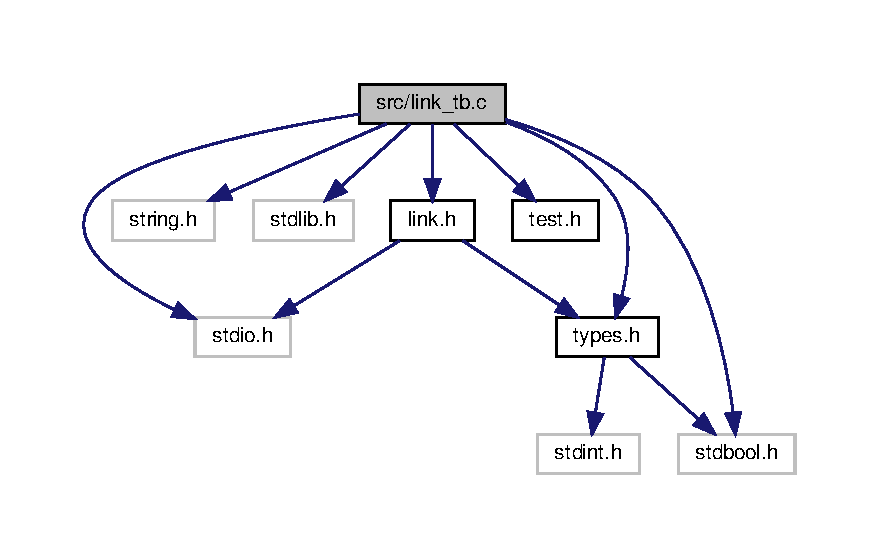
\includegraphics[width=350pt]{link__tb_8c__incl}
\end{center}
\end{figure}
\subsection*{Data Structures}
\begin{DoxyCompactItemize}
\item 
struct \hyperlink{struct__Link}{\+\_\+\+Link}
\end{DoxyCompactItemize}
\subsection*{Macros}
\begin{DoxyCompactItemize}
\item 
\mbox{\Hypertarget{link__tb_8c_a2a77d2f2c5b698c69c19e1f8782bf709}\label{link__tb_8c_a2a77d2f2c5b698c69c19e1f8782bf709}} 
\#define {\bfseries M\+A\+X\+\_\+\+T\+E\+S\+TS}~15
\item 
\mbox{\Hypertarget{link__tb_8c_a77ceac8d6af195fe72f95f6afd87c45e}\label{link__tb_8c_a77ceac8d6af195fe72f95f6afd87c45e}} 
\#define {\bfseries ID}~1
\end{DoxyCompactItemize}
\subsection*{Functions}
\begin{DoxyCompactItemize}
\item 
void \hyperlink{link__tb_8c_aeb3f2663184f88a9323d8d785e1f3683}{test1\+\_\+\+Link\+\_\+create} ()
\begin{DoxyCompactList}\small\item\em creates a Link on an integer \end{DoxyCompactList}\item 
void \hyperlink{link__tb_8c_a53e4a13ef85966a6477dcc4215895757}{test2\+\_\+\+Link\+\_\+create} ()
\begin{DoxyCompactList}\small\item\em creates a Link on an Link \end{DoxyCompactList}\item 
void \hyperlink{link__tb_8c_ae37f04cfdbd68089ea0fbb6006cd181a}{test1\+\_\+\+Link\+\_\+set\+\_\+id} ()
\begin{DoxyCompactList}\small\item\em add an invalid id \end{DoxyCompactList}\item 
void \hyperlink{link__tb_8c_a1b2d6e91e825144f230e81eff9a6f662}{test2\+\_\+\+Link\+\_\+set\+\_\+id} ()
\begin{DoxyCompactList}\small\item\em add a valid id \end{DoxyCompactList}\item 
void \hyperlink{link__tb_8c_ac8bdb5ad144f2419f34d7498a4761d8d}{test1\+\_\+\+Link\+\_\+set\+\_\+name} ()
\begin{DoxyCompactList}\small\item\em set a valid name \end{DoxyCompactList}\item 
void \hyperlink{link__tb_8c_af7f9cda1060622ad823e91458ed766cb}{test2\+\_\+\+Link\+\_\+set\+\_\+name} ()
\begin{DoxyCompactList}\small\item\em set an invalid name \end{DoxyCompactList}\item 
void \hyperlink{link__tb_8c_aa8e7315d7251d80aca226eaefa69a721}{test1\+\_\+\+Link\+\_\+set\+\_\+to} ()
\begin{DoxyCompactList}\small\item\em set an invalid to \end{DoxyCompactList}\item 
void \hyperlink{link__tb_8c_a76f0837f797222f8dcb67da889f1e05c}{test2\+\_\+\+Link\+\_\+set\+\_\+to} ()
\begin{DoxyCompactList}\small\item\em set a valid to \end{DoxyCompactList}\item 
void \hyperlink{link__tb_8c_a829e9a729c47c9d048600fc2c4cb83d9}{test1\+\_\+\+Link\+\_\+set\+\_\+from} ()
\begin{DoxyCompactList}\small\item\em get an ininvalid from \end{DoxyCompactList}\item 
void \hyperlink{link__tb_8c_af6d79d724af1e62281d0bf3a3abb709d}{test2\+\_\+\+Link\+\_\+set\+\_\+from} ()
\begin{DoxyCompactList}\small\item\em set a valid from \end{DoxyCompactList}\item 
void \hyperlink{link__tb_8c_a1826e366c041a872bd8ef260e1317c2b}{test1\+\_\+\+Link\+\_\+set\+\_\+state} ()
\begin{DoxyCompactList}\small\item\em get an invalid state \end{DoxyCompactList}\item 
void \hyperlink{link__tb_8c_a243f5384fc1bb4a71c41fb80e5437e62}{test2\+\_\+\+Link\+\_\+set\+\_\+state} ()
\begin{DoxyCompactList}\small\item\em seta a valid state \end{DoxyCompactList}\item 
void \hyperlink{link__tb_8c_a98dcb148f07ee8c2ea8494c103cd3f63}{test1\+\_\+\+Link\+\_\+print} ()
\begin{DoxyCompactList}\small\item\em print an invalid link \end{DoxyCompactList}\item 
void \hyperlink{link__tb_8c_a3852e51267b20f4d7650c9ddc0fd4025}{test2\+\_\+\+Link\+\_\+print} ()
\begin{DoxyCompactList}\small\item\em print a valid link \end{DoxyCompactList}\item 
void \hyperlink{link__tb_8c_ab1433ae001c9fa7178b34edf28ff5916}{test1\+\_\+\+Link\+\_\+get\+\_\+id} ()
\begin{DoxyCompactList}\small\item\em print a valid link \end{DoxyCompactList}\item 
void \hyperlink{link__tb_8c_a58a512428194b0f83973b221fceb1b1f}{test2\+\_\+\+Link\+\_\+get\+\_\+id} ()
\begin{DoxyCompactList}\small\item\em compares the value setted and the getted \end{DoxyCompactList}\item 
void \hyperlink{link__tb_8c_ae4ffb28986eb917fc188b2b6234f7b90}{test1\+\_\+\+Link\+\_\+get\+\_\+to} ()
\begin{DoxyCompactList}\small\item\em compares the value setted and the getted \end{DoxyCompactList}\item 
void \hyperlink{link__tb_8c_a608afd45fbc7e7e40f0c20e387059738}{test2\+\_\+\+Link\+\_\+get\+\_\+to} ()
\begin{DoxyCompactList}\small\item\em compares the value setted and the getted \end{DoxyCompactList}\item 
void \hyperlink{link__tb_8c_ad9d071835574a5da1e2fc6975fb5bd50}{test1\+\_\+\+Link\+\_\+get\+\_\+from} ()
\begin{DoxyCompactList}\small\item\em compares the value setted and the getted \end{DoxyCompactList}\item 
void \hyperlink{link__tb_8c_afa54b50b317cbfd07136184fb4843590}{test2\+\_\+\+Link\+\_\+get\+\_\+from} ()
\begin{DoxyCompactList}\small\item\em compares the value setted and the getted \end{DoxyCompactList}\item 
void \hyperlink{link__tb_8c_ae3030a87b59f46a2922136e5f574b99a}{test1\+\_\+\+Link\+\_\+get\+\_\+state} ()
\begin{DoxyCompactList}\small\item\em compares the value setted and the getted \end{DoxyCompactList}\item 
void \hyperlink{link__tb_8c_a8ac218f6799175e70309dfc8efbbb9b3}{test2\+\_\+\+Link\+\_\+get\+\_\+state} ()
\begin{DoxyCompactList}\small\item\em compares the value setted and the getted \end{DoxyCompactList}\item 
int \hyperlink{link__tb_8c_a3c04138a5bfe5d72780bb7e82a18e627}{main} (int argc, char $\ast$$\ast$argv)
\begin{DoxyCompactList}\small\item\em Funcion principal de pruebas para el modulo Link. \end{DoxyCompactList}\end{DoxyCompactItemize}


\subsection{Detailed Description}
Main for test the link. 

\begin{DoxyAuthor}{Author}
Gonzalo Serrano 
\end{DoxyAuthor}
\begin{DoxyVersion}{Version}
1.\+0 
\end{DoxyVersion}
\begin{DoxyDate}{Date}
18/03/2019 
\end{DoxyDate}


\subsection{Function Documentation}
\mbox{\Hypertarget{link__tb_8c_aeb3f2663184f88a9323d8d785e1f3683}\label{link__tb_8c_aeb3f2663184f88a9323d8d785e1f3683}} 
\index{link\+\_\+tb.\+c@{link\+\_\+tb.\+c}!test1\+\_\+\+Link\+\_\+create@{test1\+\_\+\+Link\+\_\+create}}
\index{test1\+\_\+\+Link\+\_\+create@{test1\+\_\+\+Link\+\_\+create}!link\+\_\+tb.\+c@{link\+\_\+tb.\+c}}
\subsubsection{\texorpdfstring{test1\+\_\+\+Link\+\_\+create()}{test1\_Link\_create()}}
{\footnotesize\ttfamily void test1\+\_\+\+Link\+\_\+create (\begin{DoxyParamCaption}{ }\end{DoxyParamCaption})}



creates a Link on an integer 

\begin{DoxyAuthor}{Author}
Gonzalo Serrano 
\end{DoxyAuthor}

\begin{DoxyParams}{Parameters}
{\em \{void\}} & \\
\hline
\end{DoxyParams}

\begin{DoxyRetVals}{Return values}
{\em \{void\}} & \\
\hline
\end{DoxyRetVals}
\mbox{\Hypertarget{link__tb_8c_a53e4a13ef85966a6477dcc4215895757}\label{link__tb_8c_a53e4a13ef85966a6477dcc4215895757}} 
\index{link\+\_\+tb.\+c@{link\+\_\+tb.\+c}!test2\+\_\+\+Link\+\_\+create@{test2\+\_\+\+Link\+\_\+create}}
\index{test2\+\_\+\+Link\+\_\+create@{test2\+\_\+\+Link\+\_\+create}!link\+\_\+tb.\+c@{link\+\_\+tb.\+c}}
\subsubsection{\texorpdfstring{test2\+\_\+\+Link\+\_\+create()}{test2\_Link\_create()}}
{\footnotesize\ttfamily void test2\+\_\+\+Link\+\_\+create (\begin{DoxyParamCaption}{ }\end{DoxyParamCaption})}



creates a Link on an Link 

\begin{DoxyAuthor}{Author}
Gonzalo Serrano 
\end{DoxyAuthor}

\begin{DoxyParams}{Parameters}
{\em \{void\}} & \\
\hline
\end{DoxyParams}

\begin{DoxyRetVals}{Return values}
{\em \{void\}} & \\
\hline
\end{DoxyRetVals}
\mbox{\Hypertarget{link__tb_8c_ae37f04cfdbd68089ea0fbb6006cd181a}\label{link__tb_8c_ae37f04cfdbd68089ea0fbb6006cd181a}} 
\index{link\+\_\+tb.\+c@{link\+\_\+tb.\+c}!test1\+\_\+\+Link\+\_\+set\+\_\+id@{test1\+\_\+\+Link\+\_\+set\+\_\+id}}
\index{test1\+\_\+\+Link\+\_\+set\+\_\+id@{test1\+\_\+\+Link\+\_\+set\+\_\+id}!link\+\_\+tb.\+c@{link\+\_\+tb.\+c}}
\subsubsection{\texorpdfstring{test1\+\_\+\+Link\+\_\+set\+\_\+id()}{test1\_Link\_set\_id()}}
{\footnotesize\ttfamily void test1\+\_\+\+Link\+\_\+set\+\_\+id (\begin{DoxyParamCaption}{ }\end{DoxyParamCaption})}



add an invalid id 

\begin{DoxyAuthor}{Author}
Gonzalo Serrano 
\end{DoxyAuthor}

\begin{DoxyParams}{Parameters}
{\em \{void\}} & \\
\hline
\end{DoxyParams}

\begin{DoxyRetVals}{Return values}
{\em \{void\}} & \\
\hline
\end{DoxyRetVals}
\mbox{\Hypertarget{link__tb_8c_a1b2d6e91e825144f230e81eff9a6f662}\label{link__tb_8c_a1b2d6e91e825144f230e81eff9a6f662}} 
\index{link\+\_\+tb.\+c@{link\+\_\+tb.\+c}!test2\+\_\+\+Link\+\_\+set\+\_\+id@{test2\+\_\+\+Link\+\_\+set\+\_\+id}}
\index{test2\+\_\+\+Link\+\_\+set\+\_\+id@{test2\+\_\+\+Link\+\_\+set\+\_\+id}!link\+\_\+tb.\+c@{link\+\_\+tb.\+c}}
\subsubsection{\texorpdfstring{test2\+\_\+\+Link\+\_\+set\+\_\+id()}{test2\_Link\_set\_id()}}
{\footnotesize\ttfamily void test2\+\_\+\+Link\+\_\+set\+\_\+id (\begin{DoxyParamCaption}{ }\end{DoxyParamCaption})}



add a valid id 

\begin{DoxyAuthor}{Author}
Gonzalo Serrano 
\end{DoxyAuthor}

\begin{DoxyParams}{Parameters}
{\em \{void\}} & \\
\hline
\end{DoxyParams}

\begin{DoxyRetVals}{Return values}
{\em \{void\}} & \\
\hline
\end{DoxyRetVals}
\mbox{\Hypertarget{link__tb_8c_ac8bdb5ad144f2419f34d7498a4761d8d}\label{link__tb_8c_ac8bdb5ad144f2419f34d7498a4761d8d}} 
\index{link\+\_\+tb.\+c@{link\+\_\+tb.\+c}!test1\+\_\+\+Link\+\_\+set\+\_\+name@{test1\+\_\+\+Link\+\_\+set\+\_\+name}}
\index{test1\+\_\+\+Link\+\_\+set\+\_\+name@{test1\+\_\+\+Link\+\_\+set\+\_\+name}!link\+\_\+tb.\+c@{link\+\_\+tb.\+c}}
\subsubsection{\texorpdfstring{test1\+\_\+\+Link\+\_\+set\+\_\+name()}{test1\_Link\_set\_name()}}
{\footnotesize\ttfamily void test1\+\_\+\+Link\+\_\+set\+\_\+name (\begin{DoxyParamCaption}{ }\end{DoxyParamCaption})}



set a valid name 

\begin{DoxyAuthor}{Author}
Gonzalo Serrano 
\end{DoxyAuthor}

\begin{DoxyParams}{Parameters}
{\em \{void\}} & \\
\hline
\end{DoxyParams}

\begin{DoxyRetVals}{Return values}
{\em \{void\}} & \\
\hline
\end{DoxyRetVals}
\mbox{\Hypertarget{link__tb_8c_af7f9cda1060622ad823e91458ed766cb}\label{link__tb_8c_af7f9cda1060622ad823e91458ed766cb}} 
\index{link\+\_\+tb.\+c@{link\+\_\+tb.\+c}!test2\+\_\+\+Link\+\_\+set\+\_\+name@{test2\+\_\+\+Link\+\_\+set\+\_\+name}}
\index{test2\+\_\+\+Link\+\_\+set\+\_\+name@{test2\+\_\+\+Link\+\_\+set\+\_\+name}!link\+\_\+tb.\+c@{link\+\_\+tb.\+c}}
\subsubsection{\texorpdfstring{test2\+\_\+\+Link\+\_\+set\+\_\+name()}{test2\_Link\_set\_name()}}
{\footnotesize\ttfamily void test2\+\_\+\+Link\+\_\+set\+\_\+name (\begin{DoxyParamCaption}{ }\end{DoxyParamCaption})}



set an invalid name 

\begin{DoxyAuthor}{Author}
Gonzalo Serrano 
\end{DoxyAuthor}

\begin{DoxyParams}{Parameters}
{\em \{void\}} & \\
\hline
\end{DoxyParams}

\begin{DoxyRetVals}{Return values}
{\em \{void\}} & \\
\hline
\end{DoxyRetVals}
\mbox{\Hypertarget{link__tb_8c_aa8e7315d7251d80aca226eaefa69a721}\label{link__tb_8c_aa8e7315d7251d80aca226eaefa69a721}} 
\index{link\+\_\+tb.\+c@{link\+\_\+tb.\+c}!test1\+\_\+\+Link\+\_\+set\+\_\+to@{test1\+\_\+\+Link\+\_\+set\+\_\+to}}
\index{test1\+\_\+\+Link\+\_\+set\+\_\+to@{test1\+\_\+\+Link\+\_\+set\+\_\+to}!link\+\_\+tb.\+c@{link\+\_\+tb.\+c}}
\subsubsection{\texorpdfstring{test1\+\_\+\+Link\+\_\+set\+\_\+to()}{test1\_Link\_set\_to()}}
{\footnotesize\ttfamily void test1\+\_\+\+Link\+\_\+set\+\_\+to (\begin{DoxyParamCaption}{ }\end{DoxyParamCaption})}



set an invalid to 

\begin{DoxyAuthor}{Author}
Gonzalo Serrano 
\end{DoxyAuthor}

\begin{DoxyParams}{Parameters}
{\em \{void\}} & \\
\hline
\end{DoxyParams}

\begin{DoxyRetVals}{Return values}
{\em \{void\}} & \\
\hline
\end{DoxyRetVals}
\mbox{\Hypertarget{link__tb_8c_a76f0837f797222f8dcb67da889f1e05c}\label{link__tb_8c_a76f0837f797222f8dcb67da889f1e05c}} 
\index{link\+\_\+tb.\+c@{link\+\_\+tb.\+c}!test2\+\_\+\+Link\+\_\+set\+\_\+to@{test2\+\_\+\+Link\+\_\+set\+\_\+to}}
\index{test2\+\_\+\+Link\+\_\+set\+\_\+to@{test2\+\_\+\+Link\+\_\+set\+\_\+to}!link\+\_\+tb.\+c@{link\+\_\+tb.\+c}}
\subsubsection{\texorpdfstring{test2\+\_\+\+Link\+\_\+set\+\_\+to()}{test2\_Link\_set\_to()}}
{\footnotesize\ttfamily void test2\+\_\+\+Link\+\_\+set\+\_\+to (\begin{DoxyParamCaption}{ }\end{DoxyParamCaption})}



set a valid to 

\begin{DoxyAuthor}{Author}
Gonzalo Serrano 
\end{DoxyAuthor}

\begin{DoxyParams}{Parameters}
{\em \{void\}} & \\
\hline
\end{DoxyParams}

\begin{DoxyRetVals}{Return values}
{\em \{void\}} & \\
\hline
\end{DoxyRetVals}
\mbox{\Hypertarget{link__tb_8c_a829e9a729c47c9d048600fc2c4cb83d9}\label{link__tb_8c_a829e9a729c47c9d048600fc2c4cb83d9}} 
\index{link\+\_\+tb.\+c@{link\+\_\+tb.\+c}!test1\+\_\+\+Link\+\_\+set\+\_\+from@{test1\+\_\+\+Link\+\_\+set\+\_\+from}}
\index{test1\+\_\+\+Link\+\_\+set\+\_\+from@{test1\+\_\+\+Link\+\_\+set\+\_\+from}!link\+\_\+tb.\+c@{link\+\_\+tb.\+c}}
\subsubsection{\texorpdfstring{test1\+\_\+\+Link\+\_\+set\+\_\+from()}{test1\_Link\_set\_from()}}
{\footnotesize\ttfamily void test1\+\_\+\+Link\+\_\+set\+\_\+from (\begin{DoxyParamCaption}{ }\end{DoxyParamCaption})}



get an ininvalid from 

\begin{DoxyAuthor}{Author}
Gonzalo Serrano 
\end{DoxyAuthor}

\begin{DoxyParams}{Parameters}
{\em \{void\}} & \\
\hline
\end{DoxyParams}

\begin{DoxyRetVals}{Return values}
{\em \{void\}} & \\
\hline
\end{DoxyRetVals}
\mbox{\Hypertarget{link__tb_8c_af6d79d724af1e62281d0bf3a3abb709d}\label{link__tb_8c_af6d79d724af1e62281d0bf3a3abb709d}} 
\index{link\+\_\+tb.\+c@{link\+\_\+tb.\+c}!test2\+\_\+\+Link\+\_\+set\+\_\+from@{test2\+\_\+\+Link\+\_\+set\+\_\+from}}
\index{test2\+\_\+\+Link\+\_\+set\+\_\+from@{test2\+\_\+\+Link\+\_\+set\+\_\+from}!link\+\_\+tb.\+c@{link\+\_\+tb.\+c}}
\subsubsection{\texorpdfstring{test2\+\_\+\+Link\+\_\+set\+\_\+from()}{test2\_Link\_set\_from()}}
{\footnotesize\ttfamily void test2\+\_\+\+Link\+\_\+set\+\_\+from (\begin{DoxyParamCaption}{ }\end{DoxyParamCaption})}



set a valid from 

\begin{DoxyAuthor}{Author}
Gonzalo Serrano 
\end{DoxyAuthor}

\begin{DoxyParams}{Parameters}
{\em \{void\}} & \\
\hline
\end{DoxyParams}

\begin{DoxyRetVals}{Return values}
{\em \{void\}} & \\
\hline
\end{DoxyRetVals}
\mbox{\Hypertarget{link__tb_8c_a1826e366c041a872bd8ef260e1317c2b}\label{link__tb_8c_a1826e366c041a872bd8ef260e1317c2b}} 
\index{link\+\_\+tb.\+c@{link\+\_\+tb.\+c}!test1\+\_\+\+Link\+\_\+set\+\_\+state@{test1\+\_\+\+Link\+\_\+set\+\_\+state}}
\index{test1\+\_\+\+Link\+\_\+set\+\_\+state@{test1\+\_\+\+Link\+\_\+set\+\_\+state}!link\+\_\+tb.\+c@{link\+\_\+tb.\+c}}
\subsubsection{\texorpdfstring{test1\+\_\+\+Link\+\_\+set\+\_\+state()}{test1\_Link\_set\_state()}}
{\footnotesize\ttfamily void test1\+\_\+\+Link\+\_\+set\+\_\+state (\begin{DoxyParamCaption}{ }\end{DoxyParamCaption})}



get an invalid state 

\begin{DoxyAuthor}{Author}
Gonzalo Serrano 
\end{DoxyAuthor}

\begin{DoxyParams}{Parameters}
{\em \{void\}} & \\
\hline
\end{DoxyParams}

\begin{DoxyRetVals}{Return values}
{\em \{void\}} & \\
\hline
\end{DoxyRetVals}
\mbox{\Hypertarget{link__tb_8c_a243f5384fc1bb4a71c41fb80e5437e62}\label{link__tb_8c_a243f5384fc1bb4a71c41fb80e5437e62}} 
\index{link\+\_\+tb.\+c@{link\+\_\+tb.\+c}!test2\+\_\+\+Link\+\_\+set\+\_\+state@{test2\+\_\+\+Link\+\_\+set\+\_\+state}}
\index{test2\+\_\+\+Link\+\_\+set\+\_\+state@{test2\+\_\+\+Link\+\_\+set\+\_\+state}!link\+\_\+tb.\+c@{link\+\_\+tb.\+c}}
\subsubsection{\texorpdfstring{test2\+\_\+\+Link\+\_\+set\+\_\+state()}{test2\_Link\_set\_state()}}
{\footnotesize\ttfamily void test2\+\_\+\+Link\+\_\+set\+\_\+state (\begin{DoxyParamCaption}{ }\end{DoxyParamCaption})}



seta a valid state 

\begin{DoxyAuthor}{Author}
Gonzalo Serrano 
\end{DoxyAuthor}

\begin{DoxyParams}{Parameters}
{\em \{void\}} & \\
\hline
\end{DoxyParams}

\begin{DoxyRetVals}{Return values}
{\em \{void\}} & \\
\hline
\end{DoxyRetVals}
\mbox{\Hypertarget{link__tb_8c_a98dcb148f07ee8c2ea8494c103cd3f63}\label{link__tb_8c_a98dcb148f07ee8c2ea8494c103cd3f63}} 
\index{link\+\_\+tb.\+c@{link\+\_\+tb.\+c}!test1\+\_\+\+Link\+\_\+print@{test1\+\_\+\+Link\+\_\+print}}
\index{test1\+\_\+\+Link\+\_\+print@{test1\+\_\+\+Link\+\_\+print}!link\+\_\+tb.\+c@{link\+\_\+tb.\+c}}
\subsubsection{\texorpdfstring{test1\+\_\+\+Link\+\_\+print()}{test1\_Link\_print()}}
{\footnotesize\ttfamily void test1\+\_\+\+Link\+\_\+print (\begin{DoxyParamCaption}{ }\end{DoxyParamCaption})}



print an invalid link 

\begin{DoxyAuthor}{Author}
Gonzalo Serrano 
\end{DoxyAuthor}

\begin{DoxyParams}{Parameters}
{\em \{void\}} & \\
\hline
\end{DoxyParams}

\begin{DoxyRetVals}{Return values}
{\em \{void\}} & \\
\hline
\end{DoxyRetVals}
\mbox{\Hypertarget{link__tb_8c_a3852e51267b20f4d7650c9ddc0fd4025}\label{link__tb_8c_a3852e51267b20f4d7650c9ddc0fd4025}} 
\index{link\+\_\+tb.\+c@{link\+\_\+tb.\+c}!test2\+\_\+\+Link\+\_\+print@{test2\+\_\+\+Link\+\_\+print}}
\index{test2\+\_\+\+Link\+\_\+print@{test2\+\_\+\+Link\+\_\+print}!link\+\_\+tb.\+c@{link\+\_\+tb.\+c}}
\subsubsection{\texorpdfstring{test2\+\_\+\+Link\+\_\+print()}{test2\_Link\_print()}}
{\footnotesize\ttfamily void test2\+\_\+\+Link\+\_\+print (\begin{DoxyParamCaption}{ }\end{DoxyParamCaption})}



print a valid link 

\begin{DoxyAuthor}{Author}
Gonzalo Serrano 
\end{DoxyAuthor}

\begin{DoxyParams}{Parameters}
{\em \{void\}} & \\
\hline
\end{DoxyParams}

\begin{DoxyRetVals}{Return values}
{\em \{void\}} & \\
\hline
\end{DoxyRetVals}
\mbox{\Hypertarget{link__tb_8c_ab1433ae001c9fa7178b34edf28ff5916}\label{link__tb_8c_ab1433ae001c9fa7178b34edf28ff5916}} 
\index{link\+\_\+tb.\+c@{link\+\_\+tb.\+c}!test1\+\_\+\+Link\+\_\+get\+\_\+id@{test1\+\_\+\+Link\+\_\+get\+\_\+id}}
\index{test1\+\_\+\+Link\+\_\+get\+\_\+id@{test1\+\_\+\+Link\+\_\+get\+\_\+id}!link\+\_\+tb.\+c@{link\+\_\+tb.\+c}}
\subsubsection{\texorpdfstring{test1\+\_\+\+Link\+\_\+get\+\_\+id()}{test1\_Link\_get\_id()}}
{\footnotesize\ttfamily void test1\+\_\+\+Link\+\_\+get\+\_\+id (\begin{DoxyParamCaption}{ }\end{DoxyParamCaption})}



print a valid link 

\begin{DoxyAuthor}{Author}
Gonzalo Serrano 
\end{DoxyAuthor}

\begin{DoxyParams}{Parameters}
{\em \{void\}} & \\
\hline
\end{DoxyParams}

\begin{DoxyRetVals}{Return values}
{\em \{void\}} & \\
\hline
\end{DoxyRetVals}
\mbox{\Hypertarget{link__tb_8c_a58a512428194b0f83973b221fceb1b1f}\label{link__tb_8c_a58a512428194b0f83973b221fceb1b1f}} 
\index{link\+\_\+tb.\+c@{link\+\_\+tb.\+c}!test2\+\_\+\+Link\+\_\+get\+\_\+id@{test2\+\_\+\+Link\+\_\+get\+\_\+id}}
\index{test2\+\_\+\+Link\+\_\+get\+\_\+id@{test2\+\_\+\+Link\+\_\+get\+\_\+id}!link\+\_\+tb.\+c@{link\+\_\+tb.\+c}}
\subsubsection{\texorpdfstring{test2\+\_\+\+Link\+\_\+get\+\_\+id()}{test2\_Link\_get\_id()}}
{\footnotesize\ttfamily void test2\+\_\+\+Link\+\_\+get\+\_\+id (\begin{DoxyParamCaption}{ }\end{DoxyParamCaption})}



compares the value setted and the getted 

\begin{DoxyAuthor}{Author}
Gonzalo Serrano 
\end{DoxyAuthor}

\begin{DoxyParams}{Parameters}
{\em \{void\}} & \\
\hline
\end{DoxyParams}

\begin{DoxyRetVals}{Return values}
{\em \{void\}} & \\
\hline
\end{DoxyRetVals}
\mbox{\Hypertarget{link__tb_8c_ae4ffb28986eb917fc188b2b6234f7b90}\label{link__tb_8c_ae4ffb28986eb917fc188b2b6234f7b90}} 
\index{link\+\_\+tb.\+c@{link\+\_\+tb.\+c}!test1\+\_\+\+Link\+\_\+get\+\_\+to@{test1\+\_\+\+Link\+\_\+get\+\_\+to}}
\index{test1\+\_\+\+Link\+\_\+get\+\_\+to@{test1\+\_\+\+Link\+\_\+get\+\_\+to}!link\+\_\+tb.\+c@{link\+\_\+tb.\+c}}
\subsubsection{\texorpdfstring{test1\+\_\+\+Link\+\_\+get\+\_\+to()}{test1\_Link\_get\_to()}}
{\footnotesize\ttfamily void test1\+\_\+\+Link\+\_\+get\+\_\+to (\begin{DoxyParamCaption}{ }\end{DoxyParamCaption})}



compares the value setted and the getted 

\begin{DoxyAuthor}{Author}
Gonzalo Serrano 
\end{DoxyAuthor}

\begin{DoxyParams}{Parameters}
{\em \{void\}} & \\
\hline
\end{DoxyParams}

\begin{DoxyRetVals}{Return values}
{\em \{void\}} & \\
\hline
\end{DoxyRetVals}
\mbox{\Hypertarget{link__tb_8c_a608afd45fbc7e7e40f0c20e387059738}\label{link__tb_8c_a608afd45fbc7e7e40f0c20e387059738}} 
\index{link\+\_\+tb.\+c@{link\+\_\+tb.\+c}!test2\+\_\+\+Link\+\_\+get\+\_\+to@{test2\+\_\+\+Link\+\_\+get\+\_\+to}}
\index{test2\+\_\+\+Link\+\_\+get\+\_\+to@{test2\+\_\+\+Link\+\_\+get\+\_\+to}!link\+\_\+tb.\+c@{link\+\_\+tb.\+c}}
\subsubsection{\texorpdfstring{test2\+\_\+\+Link\+\_\+get\+\_\+to()}{test2\_Link\_get\_to()}}
{\footnotesize\ttfamily void test2\+\_\+\+Link\+\_\+get\+\_\+to (\begin{DoxyParamCaption}{ }\end{DoxyParamCaption})}



compares the value setted and the getted 

\begin{DoxyAuthor}{Author}
Gonzalo Serrano 
\end{DoxyAuthor}

\begin{DoxyParams}{Parameters}
{\em \{void\}} & \\
\hline
\end{DoxyParams}

\begin{DoxyRetVals}{Return values}
{\em \{void\}} & \\
\hline
\end{DoxyRetVals}
\mbox{\Hypertarget{link__tb_8c_ad9d071835574a5da1e2fc6975fb5bd50}\label{link__tb_8c_ad9d071835574a5da1e2fc6975fb5bd50}} 
\index{link\+\_\+tb.\+c@{link\+\_\+tb.\+c}!test1\+\_\+\+Link\+\_\+get\+\_\+from@{test1\+\_\+\+Link\+\_\+get\+\_\+from}}
\index{test1\+\_\+\+Link\+\_\+get\+\_\+from@{test1\+\_\+\+Link\+\_\+get\+\_\+from}!link\+\_\+tb.\+c@{link\+\_\+tb.\+c}}
\subsubsection{\texorpdfstring{test1\+\_\+\+Link\+\_\+get\+\_\+from()}{test1\_Link\_get\_from()}}
{\footnotesize\ttfamily void test1\+\_\+\+Link\+\_\+get\+\_\+from (\begin{DoxyParamCaption}{ }\end{DoxyParamCaption})}



compares the value setted and the getted 

\begin{DoxyAuthor}{Author}
Gonzalo Serrano 
\end{DoxyAuthor}

\begin{DoxyParams}{Parameters}
{\em \{void\}} & \\
\hline
\end{DoxyParams}

\begin{DoxyRetVals}{Return values}
{\em \{void\}} & \\
\hline
\end{DoxyRetVals}
\mbox{\Hypertarget{link__tb_8c_afa54b50b317cbfd07136184fb4843590}\label{link__tb_8c_afa54b50b317cbfd07136184fb4843590}} 
\index{link\+\_\+tb.\+c@{link\+\_\+tb.\+c}!test2\+\_\+\+Link\+\_\+get\+\_\+from@{test2\+\_\+\+Link\+\_\+get\+\_\+from}}
\index{test2\+\_\+\+Link\+\_\+get\+\_\+from@{test2\+\_\+\+Link\+\_\+get\+\_\+from}!link\+\_\+tb.\+c@{link\+\_\+tb.\+c}}
\subsubsection{\texorpdfstring{test2\+\_\+\+Link\+\_\+get\+\_\+from()}{test2\_Link\_get\_from()}}
{\footnotesize\ttfamily void test2\+\_\+\+Link\+\_\+get\+\_\+from (\begin{DoxyParamCaption}{ }\end{DoxyParamCaption})}



compares the value setted and the getted 

\begin{DoxyAuthor}{Author}
Gonzalo Serrano 
\end{DoxyAuthor}

\begin{DoxyParams}{Parameters}
{\em \{void\}} & \\
\hline
\end{DoxyParams}

\begin{DoxyRetVals}{Return values}
{\em \{void\}} & \\
\hline
\end{DoxyRetVals}
\mbox{\Hypertarget{link__tb_8c_ae3030a87b59f46a2922136e5f574b99a}\label{link__tb_8c_ae3030a87b59f46a2922136e5f574b99a}} 
\index{link\+\_\+tb.\+c@{link\+\_\+tb.\+c}!test1\+\_\+\+Link\+\_\+get\+\_\+state@{test1\+\_\+\+Link\+\_\+get\+\_\+state}}
\index{test1\+\_\+\+Link\+\_\+get\+\_\+state@{test1\+\_\+\+Link\+\_\+get\+\_\+state}!link\+\_\+tb.\+c@{link\+\_\+tb.\+c}}
\subsubsection{\texorpdfstring{test1\+\_\+\+Link\+\_\+get\+\_\+state()}{test1\_Link\_get\_state()}}
{\footnotesize\ttfamily void test1\+\_\+\+Link\+\_\+get\+\_\+state (\begin{DoxyParamCaption}{ }\end{DoxyParamCaption})}



compares the value setted and the getted 

\begin{DoxyAuthor}{Author}
Gonzalo Serrano 
\end{DoxyAuthor}

\begin{DoxyParams}{Parameters}
{\em \{void\}} & \\
\hline
\end{DoxyParams}

\begin{DoxyRetVals}{Return values}
{\em \{void\}} & \\
\hline
\end{DoxyRetVals}
\mbox{\Hypertarget{link__tb_8c_a8ac218f6799175e70309dfc8efbbb9b3}\label{link__tb_8c_a8ac218f6799175e70309dfc8efbbb9b3}} 
\index{link\+\_\+tb.\+c@{link\+\_\+tb.\+c}!test2\+\_\+\+Link\+\_\+get\+\_\+state@{test2\+\_\+\+Link\+\_\+get\+\_\+state}}
\index{test2\+\_\+\+Link\+\_\+get\+\_\+state@{test2\+\_\+\+Link\+\_\+get\+\_\+state}!link\+\_\+tb.\+c@{link\+\_\+tb.\+c}}
\subsubsection{\texorpdfstring{test2\+\_\+\+Link\+\_\+get\+\_\+state()}{test2\_Link\_get\_state()}}
{\footnotesize\ttfamily void test2\+\_\+\+Link\+\_\+get\+\_\+state (\begin{DoxyParamCaption}{ }\end{DoxyParamCaption})}



compares the value setted and the getted 

\begin{DoxyAuthor}{Author}
Gonzalo Serrano 
\end{DoxyAuthor}

\begin{DoxyParams}{Parameters}
{\em \{void\}} & \\
\hline
\end{DoxyParams}

\begin{DoxyRetVals}{Return values}
{\em \{void\}} & \\
\hline
\end{DoxyRetVals}
\mbox{\Hypertarget{link__tb_8c_a3c04138a5bfe5d72780bb7e82a18e627}\label{link__tb_8c_a3c04138a5bfe5d72780bb7e82a18e627}} 
\index{link\+\_\+tb.\+c@{link\+\_\+tb.\+c}!main@{main}}
\index{main@{main}!link\+\_\+tb.\+c@{link\+\_\+tb.\+c}}
\subsubsection{\texorpdfstring{main()}{main()}}
{\footnotesize\ttfamily int main (\begin{DoxyParamCaption}\item[{int}]{argc,  }\item[{char $\ast$$\ast$}]{argv }\end{DoxyParamCaption})}



Funcion principal de pruebas para el modulo Link. 

Dos modos de ejecucion\+: 1.-\/\+Si se ejecuta sin parametros se ejecutan todas las pruebas 2.-\/\+Si se ejecuta con un numero entre 1 y el numero de pruebas solo ejecuta la prueba indicada 
\hypertarget{log_8c}{}\section{src/log.c File Reference}
\label{log_8c}\index{src/log.\+c@{src/log.\+c}}


Logger.  


{\ttfamily \#include $<$stdio.\+h$>$}\newline
{\ttfamily \#include $<$stdarg.\+h$>$}\newline
{\ttfamily \#include $<$stdbool.\+h$>$}\newline
Include dependency graph for log.\+c\+:\nopagebreak
\begin{figure}[H]
\begin{center}
\leavevmode
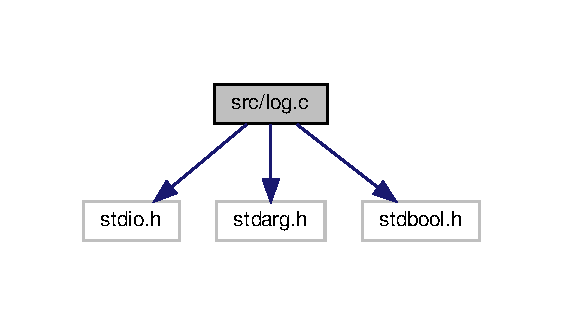
\includegraphics[width=270pt]{log_8c__incl}
\end{center}
\end{figure}
\subsection*{Functions}
\begin{DoxyCompactItemize}
\item 
bool \hyperlink{log_8c_a91c077066e868dc9488657aaf84d911d}{log\+\_\+is\+Open} ()
\begin{DoxyCompactList}\small\item\em it checks if the log file is open \end{DoxyCompactList}\item 
void \hyperlink{log_8c_a0c91588938d1cce9d3e9cb940054cd0c}{log\+\_\+begin} (const char $\ast$log\+\_\+n)
\begin{DoxyCompactList}\small\item\em initializes the file \end{DoxyCompactList}\item 
void \hyperlink{log_8c_a73e93b618b1802ac18d6e6d81b246378}{log\+\_\+end} ()
\begin{DoxyCompactList}\small\item\em it closes the file opened before \end{DoxyCompactList}\item 
void \hyperlink{log_8c_a364f0afe48f0446c287eb861e30672e5}{log\+\_\+w} (const char $\ast$frm,...)
\begin{DoxyCompactList}\small\item\em writes in the file \end{DoxyCompactList}\end{DoxyCompactItemize}
\subsection*{Variables}
\begin{DoxyCompactItemize}
\item 
\mbox{\Hypertarget{log_8c_a12b44d385fe1d1ec176c193744022600}\label{log_8c_a12b44d385fe1d1ec176c193744022600}} 
F\+I\+LE $\ast$ {\bfseries L\+O\+G\+\_\+\+F\+I\+LE} = N\+U\+LL
\end{DoxyCompactItemize}


\subsection{Detailed Description}
Logger. 

\begin{DoxyVersion}{Version}
0.\+3.\+3 
\end{DoxyVersion}
\begin{DoxyDate}{Date}
16/02/2019 
\end{DoxyDate}
\begin{DoxyAuthor}{Author}
Javier Romera 
\end{DoxyAuthor}
\begin{DoxyCopyright}{Copyright}
G\+NU Public License 
\end{DoxyCopyright}


\subsection{Function Documentation}
\mbox{\Hypertarget{log_8c_a91c077066e868dc9488657aaf84d911d}\label{log_8c_a91c077066e868dc9488657aaf84d911d}} 
\index{log.\+c@{log.\+c}!log\+\_\+is\+Open@{log\+\_\+is\+Open}}
\index{log\+\_\+is\+Open@{log\+\_\+is\+Open}!log.\+c@{log.\+c}}
\subsubsection{\texorpdfstring{log\+\_\+is\+Open()}{log\_isOpen()}}
{\footnotesize\ttfamily bool log\+\_\+is\+Open (\begin{DoxyParamCaption}{ }\end{DoxyParamCaption})}



it checks if the log file is open 

\begin{DoxyDate}{Date}
16/02/2019 
\end{DoxyDate}
\begin{DoxyAuthor}{Author}
Javier Romera
\end{DoxyAuthor}

\begin{DoxyParams}{Parameters}
{\em empty} & \\
\hline
\end{DoxyParams}

\begin{DoxyRetVals}{Return values}
{\em \{bool\}} & -\/ Returns False or True \\
\hline
\end{DoxyRetVals}
\mbox{\Hypertarget{log_8c_a0c91588938d1cce9d3e9cb940054cd0c}\label{log_8c_a0c91588938d1cce9d3e9cb940054cd0c}} 
\index{log.\+c@{log.\+c}!log\+\_\+begin@{log\+\_\+begin}}
\index{log\+\_\+begin@{log\+\_\+begin}!log.\+c@{log.\+c}}
\subsubsection{\texorpdfstring{log\+\_\+begin()}{log\_begin()}}
{\footnotesize\ttfamily void log\+\_\+begin (\begin{DoxyParamCaption}\item[{const char $\ast$}]{log\+\_\+n }\end{DoxyParamCaption})}



initializes the file 

\begin{DoxyDate}{Date}
16/02/2019 
\end{DoxyDate}
\begin{DoxyAuthor}{Author}
Javier Romera
\end{DoxyAuthor}

\begin{DoxyParams}{Parameters}
{\em \{const} & char$\ast$\} log\+\_\+n -\/ Log name \\
\hline
\end{DoxyParams}
\mbox{\Hypertarget{log_8c_a73e93b618b1802ac18d6e6d81b246378}\label{log_8c_a73e93b618b1802ac18d6e6d81b246378}} 
\index{log.\+c@{log.\+c}!log\+\_\+end@{log\+\_\+end}}
\index{log\+\_\+end@{log\+\_\+end}!log.\+c@{log.\+c}}
\subsubsection{\texorpdfstring{log\+\_\+end()}{log\_end()}}
{\footnotesize\ttfamily void log\+\_\+end (\begin{DoxyParamCaption}{ }\end{DoxyParamCaption})}



it closes the file opened before 

\begin{DoxyDate}{Date}
16/02/2019 
\end{DoxyDate}
\begin{DoxyAuthor}{Author}
Javier Romera 
\end{DoxyAuthor}

\begin{DoxyParams}{Parameters}
{\em \{char$\ast$\}} & frm -\/ String format \\
\hline
{\em \{...\}} & -\/ String format arguments \\
\hline
\end{DoxyParams}
\mbox{\Hypertarget{log_8c_a364f0afe48f0446c287eb861e30672e5}\label{log_8c_a364f0afe48f0446c287eb861e30672e5}} 
\index{log.\+c@{log.\+c}!log\+\_\+w@{log\+\_\+w}}
\index{log\+\_\+w@{log\+\_\+w}!log.\+c@{log.\+c}}
\subsubsection{\texorpdfstring{log\+\_\+w()}{log\_w()}}
{\footnotesize\ttfamily void log\+\_\+w (\begin{DoxyParamCaption}\item[{const char $\ast$}]{frm,  }\item[{}]{... }\end{DoxyParamCaption})}



writes in the file 

\begin{DoxyDate}{Date}
16/02/2019 
\end{DoxyDate}
\begin{DoxyAuthor}{Author}
Javier Romera
\end{DoxyAuthor}

\begin{DoxyParams}{Parameters}
{\em \{const} & char$\ast$\} frm -\/ String format \\
\hline
{\em \{...\}} & -\/ String format arguments \\
\hline
\end{DoxyParams}

\hypertarget{object_8c}{}\section{src/object.c File Reference}
\label{object_8c}\index{src/object.\+c@{src/object.\+c}}


Manages the game objects.  


{\ttfamily \#include \char`\"{}object.\+h\char`\"{}}\newline
{\ttfamily \#include $<$stdio.\+h$>$}\newline
{\ttfamily \#include $<$stdlib.\+h$>$}\newline
{\ttfamily \#include $<$string.\+h$>$}\newline
Include dependency graph for object.\+c\+:\nopagebreak
\begin{figure}[H]
\begin{center}
\leavevmode
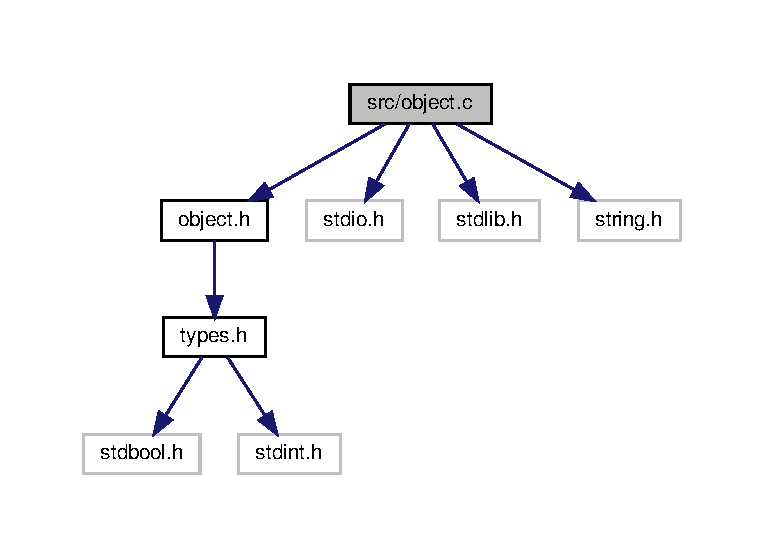
\includegraphics[width=350pt]{object_8c__incl}
\end{center}
\end{figure}
\subsection*{Data Structures}
\begin{DoxyCompactItemize}
\item 
struct \hyperlink{struct__Object}{\+\_\+\+Object}
\begin{DoxyCompactList}\small\item\em Main object structure. \end{DoxyCompactList}\end{DoxyCompactItemize}
\subsection*{Functions}
\begin{DoxyCompactItemize}
\item 
\mbox{\Hypertarget{object_8c_a1196be6af8524bec98758a054f146c66}\label{object_8c_a1196be6af8524bec98758a054f146c66}} 
Object $\ast$ {\bfseries obj\+\_\+create} (Id id)
\item 
\mbox{\Hypertarget{object_8c_ac9aeb62f8e8555a59661cca384db6b47}\label{object_8c_ac9aeb62f8e8555a59661cca384db6b47}} 
void {\bfseries obj\+\_\+destroy} (Object $\ast$obj)
\item 
\mbox{\Hypertarget{object_8c_a35e89614838eaf4f660b70d8e1bb7a83}\label{object_8c_a35e89614838eaf4f660b70d8e1bb7a83}} 
void {\bfseries obj\+\_\+set\+\_\+name} (Object $\ast$obj, const char $\ast$name)
\item 
\mbox{\Hypertarget{object_8c_a9592df618edfeffbb0cf0ae098e06ac7}\label{object_8c_a9592df618edfeffbb0cf0ae098e06ac7}} 
const char $\ast$ {\bfseries obj\+\_\+get\+\_\+name} (Object $\ast$obj)
\item 
\mbox{\Hypertarget{object_8c_ae7b80516946b9ab5124d975909409f43}\label{object_8c_ae7b80516946b9ab5124d975909409f43}} 
void {\bfseries obj\+\_\+set\+\_\+descrp} (Object $\ast$obj, const char $\ast$descrp)
\item 
\mbox{\Hypertarget{object_8c_a4f5633be628368d20545ecce98f1a94a}\label{object_8c_a4f5633be628368d20545ecce98f1a94a}} 
const char $\ast$ {\bfseries obj\+\_\+get\+\_\+descrp} (Object $\ast$obj)
\item 
\mbox{\Hypertarget{object_8c_af3ca397f0f2c6784bde1f1ae5d63b7f9}\label{object_8c_af3ca397f0f2c6784bde1f1ae5d63b7f9}} 
void {\bfseries obj\+\_\+set\+\_\+id} (Object $\ast$obj, const Id id)
\item 
\mbox{\Hypertarget{object_8c_a7241dbfc246b252ee486f31519794922}\label{object_8c_a7241dbfc246b252ee486f31519794922}} 
const Id {\bfseries obj\+\_\+get\+\_\+id} (Object $\ast$obj)
\end{DoxyCompactItemize}


\subsection{Detailed Description}
Manages the game objects. 

\begin{DoxyAuthor}{Author}
Miguel Rodríguez 
\end{DoxyAuthor}
\begin{DoxyVersion}{Version}
1.\+0 
\end{DoxyVersion}
\begin{DoxyDate}{Date}
18/03/2019 
\end{DoxyDate}

\hypertarget{object__tb_8c}{}\section{src/object\+\_\+tb.c File Reference}
\label{object__tb_8c}\index{src/object\+\_\+tb.\+c@{src/object\+\_\+tb.\+c}}


Object testbench evaluates each object function for each case.  


{\ttfamily \#include \char`\"{}object.\+h\char`\"{}}\newline
{\ttfamily \#include \char`\"{}types.\+h\char`\"{}}\newline
{\ttfamily \#include \char`\"{}ui.\+h\char`\"{}}\newline
{\ttfamily \#include $<$stdio.\+h$>$}\newline
{\ttfamily \#include $<$stdlib.\+h$>$}\newline
{\ttfamily \#include $<$stdbool.\+h$>$}\newline
{\ttfamily \#include $<$time.\+h$>$}\newline
{\ttfamily \#include $<$string.\+h$>$}\newline
Include dependency graph for object\+\_\+tb.\+c\+:\nopagebreak
\begin{figure}[H]
\begin{center}
\leavevmode
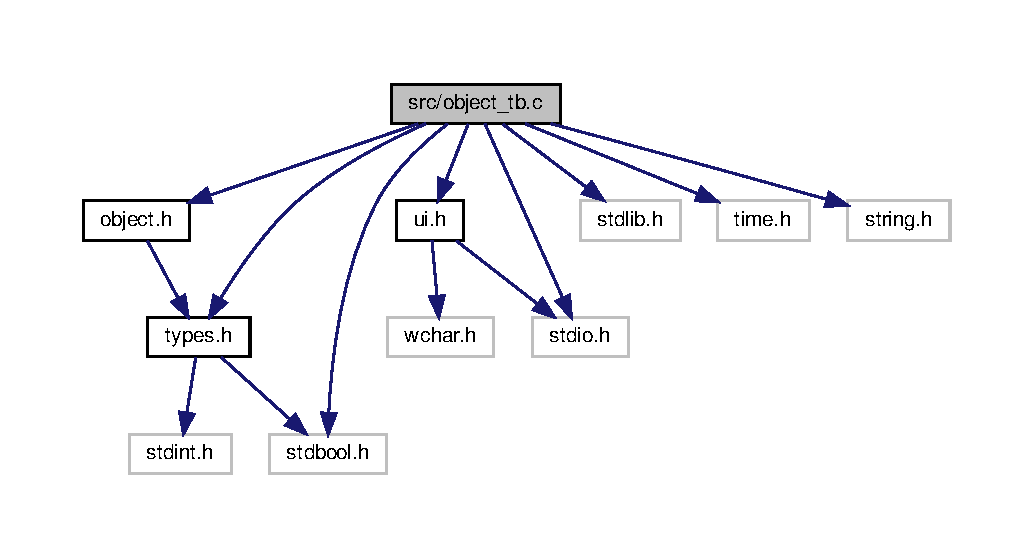
\includegraphics[width=350pt]{object__tb_8c__incl}
\end{center}
\end{figure}
\subsection*{Macros}
\begin{DoxyCompactItemize}
\item 
\mbox{\Hypertarget{object__tb_8c_a8e497c59a3362df6102c893a8498acd0}\label{object__tb_8c_a8e497c59a3362df6102c893a8498acd0}} 
\#define \hyperlink{object__tb_8c_a8e497c59a3362df6102c893a8498acd0}{M\+A\+X\+\_\+\+O\+BJ}~2
\begin{DoxyCompactList}\small\item\em Default maxumum objects. \end{DoxyCompactList}\item 
\mbox{\Hypertarget{object__tb_8c_acaf8542f12a3067d567582215362f57f}\label{object__tb_8c_acaf8542f12a3067d567582215362f57f}} 
\#define \hyperlink{object__tb_8c_acaf8542f12a3067d567582215362f57f}{E\+R\+R\+\_\+\+TB}~2
\begin{DoxyCompactList}\small\item\em Default error testbench loop. \end{DoxyCompactList}\item 
\mbox{\Hypertarget{object__tb_8c_a1224dbeb12320494fbd819c86fb3172b}\label{object__tb_8c_a1224dbeb12320494fbd819c86fb3172b}} 
\#define \hyperlink{object__tb_8c_a1224dbeb12320494fbd819c86fb3172b}{N\+A\+M\+ES}~30
\begin{DoxyCompactList}\small\item\em Default total name. \end{DoxyCompactList}\item 
\mbox{\Hypertarget{object__tb_8c_a20d54f00df3ea433cbc81291da38c38e}\label{object__tb_8c_a20d54f00df3ea433cbc81291da38c38e}} 
\#define \hyperlink{object__tb_8c_a20d54f00df3ea433cbc81291da38c38e}{D\+E\+S\+C\+R\+I\+P\+T\+I\+O\+NS}~30
\begin{DoxyCompactList}\small\item\em Default total descriptions. \end{DoxyCompactList}\end{DoxyCompactItemize}
\subsection*{Functions}
\begin{DoxyCompactItemize}
\item 
\hyperlink{types_8h_a32c27cc471df37f4fc818d65de0a56c4}{S\+T\+A\+T\+US} \hyperlink{object__tb_8c_a8539e14a647ab11baff5a4af69fdbf9f}{main\+\_\+clean} (\hyperlink{object_8h_a7f8bbcda919b65ce67f92fba08e0212f}{Object} $\ast$$\ast$objects)
\begin{DoxyCompactList}\small\item\em Cleans array passed as argument. \end{DoxyCompactList}\item 
\hyperlink{types_8h_a32c27cc471df37f4fc818d65de0a56c4}{S\+T\+A\+T\+US} \hyperlink{object__tb_8c_acb54370a852691289541f6ef0595ea8d}{main\+\_\+print} (\hyperlink{object_8h_a7f8bbcda919b65ce67f92fba08e0212f}{Object} $\ast$object)
\begin{DoxyCompactList}\small\item\em Prints object information. \end{DoxyCompactList}\item 
\hyperlink{types_8h_a32c27cc471df37f4fc818d65de0a56c4}{S\+T\+A\+T\+US} \hyperlink{object__tb_8c_abac8001e832809a2732ad62a78b888b2}{main\+\_\+valid} (\hyperlink{object_8h_a7f8bbcda919b65ce67f92fba08e0212f}{Object} $\ast$$\ast$objects)
\begin{DoxyCompactList}\small\item\em Test object module with valid values. \end{DoxyCompactList}\item 
\hyperlink{types_8h_a32c27cc471df37f4fc818d65de0a56c4}{S\+T\+A\+T\+US} \hyperlink{object__tb_8c_a140dc41d1787cefc934736a7e283e77e}{main\+\_\+err} (\hyperlink{object_8h_a7f8bbcda919b65ce67f92fba08e0212f}{Object} $\ast$$\ast$objects)
\begin{DoxyCompactList}\small\item\em Test object module with non-\/valid values. \end{DoxyCompactList}\item 
int \hyperlink{object__tb_8c_a0ddf1224851353fc92bfbff6f499fa97}{main} (int argc, char $\ast$argv\mbox{[}$\,$\mbox{]})
\begin{DoxyCompactList}\small\item\em Test main function, contains a case select. \end{DoxyCompactList}\end{DoxyCompactItemize}
\subsection*{Variables}
\begin{DoxyCompactItemize}
\item 
\mbox{\Hypertarget{object__tb_8c_acb559820d9ca11295b4500f179ef6392}\label{object__tb_8c_acb559820d9ca11295b4500f179ef6392}} 
int {\bfseries i} = 0
\item 
\mbox{\Hypertarget{object__tb_8c_acab531abaa74a7e664e3986f2522b33a}\label{object__tb_8c_acab531abaa74a7e664e3986f2522b33a}} 
int {\bfseries r} = 0
\item 
\mbox{\Hypertarget{object__tb_8c_ac310d9181e916ba43604099aee272c71}\label{object__tb_8c_ac310d9181e916ba43604099aee272c71}} 
int {\bfseries t} = 0
\item 
\mbox{\Hypertarget{object__tb_8c_a150a709e86e7134d17cd063de6810b6c}\label{object__tb_8c_a150a709e86e7134d17cd063de6810b6c}} 
\hyperlink{types_8h_a845e604fb28f7e3d97549da3448149d3}{Id} {\bfseries id} = \hyperlink{types_8h_a642e16f35aa1e585c25e405ede76e115}{N\+O\+\_\+\+ID}
\item 
\mbox{\Hypertarget{object__tb_8c_a470055fdb0cbfa3bcca1e4e17620cff5}\label{object__tb_8c_a470055fdb0cbfa3bcca1e4e17620cff5}} 
\hyperlink{types_8h_a845e604fb28f7e3d97549da3448149d3}{Id} {\bfseries name\+\_\+id} = \hyperlink{types_8h_a642e16f35aa1e585c25e405ede76e115}{N\+O\+\_\+\+ID}
\item 
\mbox{\Hypertarget{object__tb_8c_a862a2982472e549ea02e4be8bc0afd22}\label{object__tb_8c_a862a2982472e549ea02e4be8bc0afd22}} 
\hyperlink{types_8h_a845e604fb28f7e3d97549da3448149d3}{Id} {\bfseries desc\+\_\+id} = \hyperlink{types_8h_a642e16f35aa1e585c25e405ede76e115}{N\+O\+\_\+\+ID}
\item 
\mbox{\Hypertarget{object__tb_8c_af45c9328d28821aa5082827651e2a23d}\label{object__tb_8c_af45c9328d28821aa5082827651e2a23d}} 
char {\bfseries name} \mbox{[}\hyperlink{object_8h_a6a2f391825e94d06a3137b75abfa1bba}{M\+A\+X\+\_\+\+O\+B\+J\+\_\+\+N\+A\+ME}\mbox{]}
\item 
\mbox{\Hypertarget{object__tb_8c_a92c3036bcb0447e4d8ee86f9ec3c66a3}\label{object__tb_8c_a92c3036bcb0447e4d8ee86f9ec3c66a3}} 
char {\bfseries desc} \mbox{[}\hyperlink{object_8h_a9c396da2f3b9f0191120ff1666af6381}{M\+A\+X\+\_\+\+O\+B\+J\+\_\+\+D\+E\+S\+C\+RP}\mbox{]}
\item 
\mbox{\Hypertarget{object__tb_8c_a84326fa5b9d0969f0ed020ea927be3ba}\label{object__tb_8c_a84326fa5b9d0969f0ed020ea927be3ba}} 
char \hyperlink{object__tb_8c_a84326fa5b9d0969f0ed020ea927be3ba}{names} \mbox{[}\hyperlink{object__tb_8c_a1224dbeb12320494fbd819c86fb3172b}{N\+A\+M\+ES}\mbox{]}\mbox{[}\hyperlink{object_8h_a6a2f391825e94d06a3137b75abfa1bba}{M\+A\+X\+\_\+\+O\+B\+J\+\_\+\+N\+A\+ME}\mbox{]} = \{\char`\"{}Botas\char`\"{}, \char`\"{}Armadura\char`\"{}, \char`\"{}Anillo\char`\"{}, \char`\"{}Baston\char`\"{}, \char`\"{}Amuleto\char`\"{}, \char`\"{}Ancla\char`\"{}, \char`\"{}Brazalete\char`\"{}, \char`\"{}Capa\char`\"{}, \char`\"{}Pergamino\char`\"{}, \char`\"{}Eter\char`\"{}, \char`\"{}Cetro\char`\"{}, \char`\"{}Chaleco\char`\"{}, \char`\"{}Coraza\char`\"{}, \char`\"{}Cimitarra\char`\"{}, \char`\"{}Brazal\char`\"{}, \char`\"{}Cristal\char`\"{}, \char`\"{}Cinturon\char`\"{}, \char`\"{}Caliz\char`\"{}, \char`\"{}Cefiro\char`\"{}, \char`\"{}Codice\char`\"{}, \char`\"{}Cronometro\char`\"{}, \char`\"{}Daga\char`\"{}, \char`\"{}Sello\char`\"{}, \char`\"{}Elixir\char`\"{}, \char`\"{}Escudo\char`\"{}, \char`\"{}Estandarte\char`\"{}, \char`\"{}Galleta\char`\"{}, \char`\"{}Guantelete\char`\"{}, \char`\"{}Grebas\char`\"{}, \char`\"{}Reloj\char`\"{}\}
\begin{DoxyCompactList}\small\item\em Default names. \end{DoxyCompactList}\item 
\mbox{\Hypertarget{object__tb_8c_a0ac53fc0cb318098279f0900283fc8e7}\label{object__tb_8c_a0ac53fc0cb318098279f0900283fc8e7}} 
char \hyperlink{object__tb_8c_a0ac53fc0cb318098279f0900283fc8e7}{descriptions} \mbox{[}\hyperlink{object__tb_8c_a20d54f00df3ea433cbc81291da38c38e}{D\+E\+S\+C\+R\+I\+P\+T\+I\+O\+NS}\mbox{]}\mbox{[}\hyperlink{object_8h_a9c396da2f3b9f0191120ff1666af6381}{M\+A\+X\+\_\+\+O\+B\+J\+\_\+\+D\+E\+S\+C\+RP}\mbox{]} = \{\char`\"{}Para los pies\char`\"{}, \char`\"{}Para el cuerpo\char`\"{}, \char`\"{}Para el dedo\char`\"{}, \char`\"{}Para sujeccion\char`\"{}, \char`\"{}Para suerte\char`\"{}, \char`\"{}Para barco\char`\"{}, \char`\"{}Para brazo\char`\"{}, \char`\"{}Para espalda\char`\"{}, \char`\"{}Para guiarte\char`\"{}, \char`\"{}Para disolver\char`\"{}, \char`\"{}Para ataque\char`\"{}, \char`\"{}Para tiempo\char`\"{}, \char`\"{}Para proteccion\char`\"{}, \char`\"{}Para ataque\char`\"{}, \char`\"{}Para brazo\char`\"{}, \char`\"{}Para videncia\char`\"{}, \char`\"{}Para sujeccion\char`\"{}, \char`\"{}Para beber\char`\"{}, \char`\"{}Para viento\char`\"{}, \char`\"{}Para biblioteca\char`\"{}, \char`\"{}Para tiempo\char`\"{}, \char`\"{}Para ataque\char`\"{}, \char`\"{}Para carta\char`\"{}, \char`\"{}Para pocima\char`\"{}, \char`\"{}Para proteccion\char`\"{}, \char`\"{}Para comer\char`\"{}, \char`\"{}Para mano\char`\"{}, \char`\"{}Para piernas\char`\"{}, \char`\"{}Para tiempo\char`\"{}\}
\begin{DoxyCompactList}\small\item\em Default descriptions. \end{DoxyCompactList}\end{DoxyCompactItemize}


\subsection{Detailed Description}
Object testbench evaluates each object function for each case. 

Player testbench, valuates each player function for each case.

\begin{DoxyVersion}{Version}
1.\+0.\+0 
\end{DoxyVersion}
\begin{DoxyDate}{Date}
7/04/2019 
\end{DoxyDate}
\begin{DoxyAuthor}{Author}
Álvaro Rodríguez 
\end{DoxyAuthor}
\begin{DoxyCopyright}{Copyright}
G\+NU Public License
\end{DoxyCopyright}
\begin{DoxyVersion}{Version}
1.\+0.\+0 
\end{DoxyVersion}
\begin{DoxyDate}{Date}
5/04/2019 
\end{DoxyDate}
\begin{DoxyAuthor}{Author}
Álvaro Rodríguez 
\end{DoxyAuthor}
\begin{DoxyCopyright}{Copyright}
G\+NU Public License 
\end{DoxyCopyright}


\subsection{Function Documentation}
\mbox{\Hypertarget{object__tb_8c_a8539e14a647ab11baff5a4af69fdbf9f}\label{object__tb_8c_a8539e14a647ab11baff5a4af69fdbf9f}} 
\index{object\+\_\+tb.\+c@{object\+\_\+tb.\+c}!main\+\_\+clean@{main\+\_\+clean}}
\index{main\+\_\+clean@{main\+\_\+clean}!object\+\_\+tb.\+c@{object\+\_\+tb.\+c}}
\subsubsection{\texorpdfstring{main\+\_\+clean()}{main\_clean()}}
{\footnotesize\ttfamily \hyperlink{types_8h_a32c27cc471df37f4fc818d65de0a56c4}{S\+T\+A\+T\+US} main\+\_\+clean (\begin{DoxyParamCaption}\item[{\hyperlink{object_8h_a7f8bbcda919b65ce67f92fba08e0212f}{Object} $\ast$$\ast$}]{objects }\end{DoxyParamCaption})}



Cleans array passed as argument. 

\begin{DoxyAuthor}{Author}
Álvaro Rodríguez 
\end{DoxyAuthor}

\begin{DoxyParams}{Parameters}
{\em \{\+Object$\ast$$\ast$\}} & objects -\/ objects identificator \\
\hline
\end{DoxyParams}

\begin{DoxyRetVals}{Return values}
{\em Returns} & a state \\
\hline
\end{DoxyRetVals}
\mbox{\Hypertarget{object__tb_8c_acb54370a852691289541f6ef0595ea8d}\label{object__tb_8c_acb54370a852691289541f6ef0595ea8d}} 
\index{object\+\_\+tb.\+c@{object\+\_\+tb.\+c}!main\+\_\+print@{main\+\_\+print}}
\index{main\+\_\+print@{main\+\_\+print}!object\+\_\+tb.\+c@{object\+\_\+tb.\+c}}
\subsubsection{\texorpdfstring{main\+\_\+print()}{main\_print()}}
{\footnotesize\ttfamily \hyperlink{types_8h_a32c27cc471df37f4fc818d65de0a56c4}{S\+T\+A\+T\+US} main\+\_\+print (\begin{DoxyParamCaption}\item[{\hyperlink{object_8h_a7f8bbcda919b65ce67f92fba08e0212f}{Object} $\ast$}]{object }\end{DoxyParamCaption})}



Prints object information. 

\begin{DoxyAuthor}{Author}
Álvaro Rodríguez 
\end{DoxyAuthor}

\begin{DoxyParams}{Parameters}
{\em \{\+Object$\ast$\}} & objects -\/ object identificator \\
\hline
\end{DoxyParams}

\begin{DoxyRetVals}{Return values}
{\em Returns} & a state \\
\hline
\end{DoxyRetVals}
\mbox{\Hypertarget{object__tb_8c_abac8001e832809a2732ad62a78b888b2}\label{object__tb_8c_abac8001e832809a2732ad62a78b888b2}} 
\index{object\+\_\+tb.\+c@{object\+\_\+tb.\+c}!main\+\_\+valid@{main\+\_\+valid}}
\index{main\+\_\+valid@{main\+\_\+valid}!object\+\_\+tb.\+c@{object\+\_\+tb.\+c}}
\subsubsection{\texorpdfstring{main\+\_\+valid()}{main\_valid()}}
{\footnotesize\ttfamily \hyperlink{types_8h_a32c27cc471df37f4fc818d65de0a56c4}{S\+T\+A\+T\+US} main\+\_\+valid (\begin{DoxyParamCaption}\item[{\hyperlink{object_8h_a7f8bbcda919b65ce67f92fba08e0212f}{Object} $\ast$$\ast$}]{objects }\end{DoxyParamCaption})}



Test object module with valid values. 

\begin{DoxyAuthor}{Author}
Álvaro Rodríguez 
\end{DoxyAuthor}

\begin{DoxyParams}{Parameters}
{\em \{\+Object$\ast$$\ast$\}} & objects -\/ objects identificator \\
\hline
\end{DoxyParams}

\begin{DoxyRetVals}{Return values}
{\em Returns} & a state \\
\hline
\end{DoxyRetVals}
\mbox{\Hypertarget{object__tb_8c_a140dc41d1787cefc934736a7e283e77e}\label{object__tb_8c_a140dc41d1787cefc934736a7e283e77e}} 
\index{object\+\_\+tb.\+c@{object\+\_\+tb.\+c}!main\+\_\+err@{main\+\_\+err}}
\index{main\+\_\+err@{main\+\_\+err}!object\+\_\+tb.\+c@{object\+\_\+tb.\+c}}
\subsubsection{\texorpdfstring{main\+\_\+err()}{main\_err()}}
{\footnotesize\ttfamily \hyperlink{types_8h_a32c27cc471df37f4fc818d65de0a56c4}{S\+T\+A\+T\+US} main\+\_\+err (\begin{DoxyParamCaption}\item[{\hyperlink{object_8h_a7f8bbcda919b65ce67f92fba08e0212f}{Object} $\ast$$\ast$}]{objects }\end{DoxyParamCaption})}



Test object module with non-\/valid values. 

\begin{DoxyAuthor}{Author}
Álvaro Rodríguez 
\end{DoxyAuthor}

\begin{DoxyParams}{Parameters}
{\em \{\+Object$\ast$$\ast$\}} & objects -\/ objects identificator \\
\hline
\end{DoxyParams}

\begin{DoxyRetVals}{Return values}
{\em Returns} & a state \\
\hline
\end{DoxyRetVals}
\mbox{\Hypertarget{object__tb_8c_a0ddf1224851353fc92bfbff6f499fa97}\label{object__tb_8c_a0ddf1224851353fc92bfbff6f499fa97}} 
\index{object\+\_\+tb.\+c@{object\+\_\+tb.\+c}!main@{main}}
\index{main@{main}!object\+\_\+tb.\+c@{object\+\_\+tb.\+c}}
\subsubsection{\texorpdfstring{main()}{main()}}
{\footnotesize\ttfamily int main (\begin{DoxyParamCaption}\item[{int}]{argc,  }\item[{char $\ast$}]{argv\mbox{[}$\,$\mbox{]} }\end{DoxyParamCaption})}



Test main function, contains a case select. 

\begin{DoxyAuthor}{Author}
Álvaro Rodríguez 
\end{DoxyAuthor}

\begin{DoxyParams}{Parameters}
{\em \{int\}} & argc -\/ number of arguments \\
\hline
{\em \{int\}} & argv\mbox{[}\mbox{]} -\/ arguments \\
\hline
\end{DoxyParams}

\begin{DoxyRetVals}{Return values}
{\em Returns} & a integer \\
\hline
\end{DoxyRetVals}

\hypertarget{player_8c}{}\section{src/player.c File Reference}
\label{player_8c}\index{src/player.\+c@{src/player.\+c}}


Main player manager.  


{\ttfamily \#include \char`\"{}player.\+h\char`\"{}}\newline
{\ttfamily \#include \char`\"{}types.\+h\char`\"{}}\newline
{\ttfamily \#include \char`\"{}inventory.\+h\char`\"{}}\newline
{\ttfamily \#include $<$stdio.\+h$>$}\newline
{\ttfamily \#include $<$stdlib.\+h$>$}\newline
{\ttfamily \#include $<$string.\+h$>$}\newline
Include dependency graph for player.\+c\+:\nopagebreak
\begin{figure}[H]
\begin{center}
\leavevmode
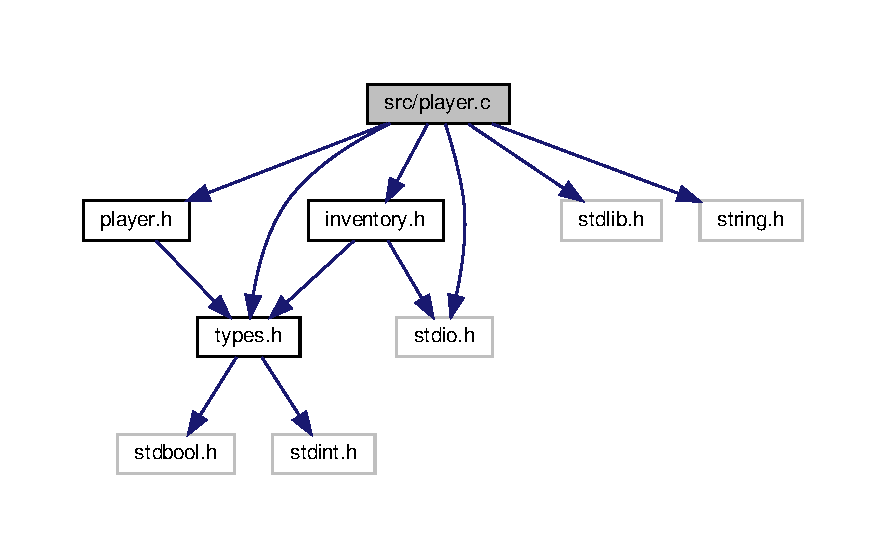
\includegraphics[width=350pt]{player_8c__incl}
\end{center}
\end{figure}
\subsection*{Data Structures}
\begin{DoxyCompactItemize}
\item 
struct \hyperlink{struct__Player}{\+\_\+\+Player}
\begin{DoxyCompactList}\small\item\em Player\textquotesingle{}s structure. \end{DoxyCompactList}\end{DoxyCompactItemize}
\subsection*{Functions}
\begin{DoxyCompactItemize}
\item 
\hyperlink{struct__Player}{Player} $\ast$ \hyperlink{player_8c_a97ea1d0deda3c51ef6ce63a13dab7a38}{player\+\_\+create} (\hyperlink{types_8h_a845e604fb28f7e3d97549da3448149d3}{Id} id)
\begin{DoxyCompactList}\small\item\em This fuction initializes a player. \end{DoxyCompactList}\item 
\hyperlink{types_8h_a32c27cc471df37f4fc818d65de0a56c4}{S\+T\+A\+T\+US} \hyperlink{player_8c_a68e324aa5064e27d0a2f38aafb6809ad}{player\+\_\+destroy} (\hyperlink{struct__Player}{Player} $\ast$player)
\begin{DoxyCompactList}\small\item\em This fuction destroys a player. \end{DoxyCompactList}\item 
\hyperlink{types_8h_a32c27cc471df37f4fc818d65de0a56c4}{S\+T\+A\+T\+US} \hyperlink{player_8c_a6a30809f7775f5c2d3bef47d92769e59}{player\+\_\+set\+\_\+name} (\hyperlink{struct__Player}{Player} $\ast$player, char $\ast$name)
\begin{DoxyCompactList}\small\item\em This fuction sets the player\textquotesingle{}s name. \end{DoxyCompactList}\item 
\hyperlink{types_8h_a32c27cc471df37f4fc818d65de0a56c4}{S\+T\+A\+T\+US} \hyperlink{player_8c_ac8ace1a1b6b11bc7f92a71a3922e4b83}{player\+\_\+set\+\_\+location} (\hyperlink{struct__Player}{Player} $\ast$player, \hyperlink{types_8h_a845e604fb28f7e3d97549da3448149d3}{Id} id)
\begin{DoxyCompactList}\small\item\em This fuction sets the player\textquotesingle{}s location. \end{DoxyCompactList}\item 
\hyperlink{types_8h_a32c27cc471df37f4fc818d65de0a56c4}{S\+T\+A\+T\+US} \hyperlink{player_8c_a2fc269feb0641f59daab5e6b77cb1a75}{player\+\_\+add\+\_\+object} (\hyperlink{struct__Player}{Player} $\ast$player, \hyperlink{types_8h_a845e604fb28f7e3d97549da3448149d3}{Id} id)
\begin{DoxyCompactList}\small\item\em This fuction adds an object to playes\textquotesingle{}s inventory. \end{DoxyCompactList}\item 
\hyperlink{types_8h_a32c27cc471df37f4fc818d65de0a56c4}{S\+T\+A\+T\+US} \hyperlink{player_8c_a68871bc282449eb64b977acbdbd7565a}{player\+\_\+del\+\_\+object} (\hyperlink{struct__Player}{Player} $\ast$player, \hyperlink{types_8h_a845e604fb28f7e3d97549da3448149d3}{Id} id)
\begin{DoxyCompactList}\small\item\em This fuction removes an object from player\textquotesingle{}s inventory. \end{DoxyCompactList}\item 
const char $\ast$ \hyperlink{player_8c_a6622c02be2fe230a5c0df66385a13ece}{player\+\_\+get\+\_\+name} (\hyperlink{struct__Player}{Player} $\ast$player)
\begin{DoxyCompactList}\small\item\em This fuction gets the palyer\textquotesingle{}s name. \end{DoxyCompactList}\item 
void \hyperlink{player_8c_a278466eff9dd013babc5bdbd485f1da0}{player\+\_\+set\+\_\+id} (\hyperlink{struct__Player}{Player} $\ast$player, \hyperlink{types_8h_a845e604fb28f7e3d97549da3448149d3}{Id} id)
\begin{DoxyCompactList}\small\item\em This fuction sets the palyer\textquotesingle{}s id. \end{DoxyCompactList}\item 
\hyperlink{types_8h_a845e604fb28f7e3d97549da3448149d3}{Id} \hyperlink{player_8c_af5a101ec91427951c5875569a8709956}{player\+\_\+get\+\_\+id} (\hyperlink{struct__Player}{Player} $\ast$player)
\begin{DoxyCompactList}\small\item\em This fuction gets the palyer\textquotesingle{}s id. \end{DoxyCompactList}\item 
\hyperlink{types_8h_a845e604fb28f7e3d97549da3448149d3}{Id} \hyperlink{player_8c_aa50ce77ab79af7166d749619fd60acfe}{player\+\_\+get\+\_\+location} (\hyperlink{struct__Player}{Player} $\ast$player)
\begin{DoxyCompactList}\small\item\em This fuction gets the palyer\textquotesingle{}s location. \end{DoxyCompactList}\item 
bool \hyperlink{player_8c_aa23cae616f2d42403a1f99fdde686f06}{player\+\_\+has\+\_\+object} (\hyperlink{struct__Player}{Player} $\ast$player, \hyperlink{types_8h_a845e604fb28f7e3d97549da3448149d3}{Id} id)
\begin{DoxyCompactList}\small\item\em This fuction searches if an object is in the player\textquotesingle{}s inventory. \end{DoxyCompactList}\end{DoxyCompactItemize}


\subsection{Detailed Description}
Main player manager. 

\begin{DoxyAuthor}{Author}
Miguel Rodríguez 
\end{DoxyAuthor}
\begin{DoxyVersion}{Version}
1.\+0 
\end{DoxyVersion}
\begin{DoxyDate}{Date}
18/03/2019 
\end{DoxyDate}


\subsection{Function Documentation}
\mbox{\Hypertarget{player_8c_a97ea1d0deda3c51ef6ce63a13dab7a38}\label{player_8c_a97ea1d0deda3c51ef6ce63a13dab7a38}} 
\index{player.\+c@{player.\+c}!player\+\_\+create@{player\+\_\+create}}
\index{player\+\_\+create@{player\+\_\+create}!player.\+c@{player.\+c}}
\subsubsection{\texorpdfstring{player\+\_\+create()}{player\_create()}}
{\footnotesize\ttfamily \hyperlink{struct__Player}{Player}$\ast$ player\+\_\+create (\begin{DoxyParamCaption}\item[{\hyperlink{types_8h_a845e604fb28f7e3d97549da3448149d3}{Id}}]{id }\end{DoxyParamCaption})}



This fuction initializes a player. 

\begin{DoxyAuthor}{Author}
Miguel Rodríguez 
\end{DoxyAuthor}

\begin{DoxyParams}{Parameters}
{\em \{\+Id\}} & -\/ Player identification \\
\hline
\end{DoxyParams}

\begin{DoxyRetVals}{Return values}
{\em \{\+Player$\ast$\}} & -\/ Returns a player\textquotesingle{}s pointer \\
\hline
\end{DoxyRetVals}
\mbox{\Hypertarget{player_8c_a68e324aa5064e27d0a2f38aafb6809ad}\label{player_8c_a68e324aa5064e27d0a2f38aafb6809ad}} 
\index{player.\+c@{player.\+c}!player\+\_\+destroy@{player\+\_\+destroy}}
\index{player\+\_\+destroy@{player\+\_\+destroy}!player.\+c@{player.\+c}}
\subsubsection{\texorpdfstring{player\+\_\+destroy()}{player\_destroy()}}
{\footnotesize\ttfamily \hyperlink{types_8h_a32c27cc471df37f4fc818d65de0a56c4}{S\+T\+A\+T\+US} player\+\_\+destroy (\begin{DoxyParamCaption}\item[{\hyperlink{struct__Player}{Player} $\ast$}]{player }\end{DoxyParamCaption})}



This fuction destroys a player. 

\begin{DoxyAuthor}{Author}
Miguel Rodríguez 
\end{DoxyAuthor}

\begin{DoxyParams}{Parameters}
{\em \{\+Player$\ast$\}} & player -\/ player\textquotesingle{}s pointer \\
\hline
\end{DoxyParams}
\mbox{\Hypertarget{player_8c_a6a30809f7775f5c2d3bef47d92769e59}\label{player_8c_a6a30809f7775f5c2d3bef47d92769e59}} 
\index{player.\+c@{player.\+c}!player\+\_\+set\+\_\+name@{player\+\_\+set\+\_\+name}}
\index{player\+\_\+set\+\_\+name@{player\+\_\+set\+\_\+name}!player.\+c@{player.\+c}}
\subsubsection{\texorpdfstring{player\+\_\+set\+\_\+name()}{player\_set\_name()}}
{\footnotesize\ttfamily \hyperlink{types_8h_a32c27cc471df37f4fc818d65de0a56c4}{S\+T\+A\+T\+US} player\+\_\+set\+\_\+name (\begin{DoxyParamCaption}\item[{\hyperlink{struct__Player}{Player} $\ast$}]{player,  }\item[{char $\ast$}]{name }\end{DoxyParamCaption})}



This fuction sets the player\textquotesingle{}s name. 

\begin{DoxyAuthor}{Author}
Miguel Rodríguez 
\end{DoxyAuthor}

\begin{DoxyParams}{Parameters}
{\em \{\+Player$\ast$\}} & player -\/ player\textquotesingle{}s pointer \\
\hline
{\em \{char$\ast$\}} & name -\/ player\textquotesingle{}s name \\
\hline
\end{DoxyParams}

\begin{DoxyRetVals}{Return values}
{\em \{\+S\+T\+A\+T\+U\+S\}} & -\/ Returns a status code \\
\hline
\end{DoxyRetVals}
\mbox{\Hypertarget{player_8c_ac8ace1a1b6b11bc7f92a71a3922e4b83}\label{player_8c_ac8ace1a1b6b11bc7f92a71a3922e4b83}} 
\index{player.\+c@{player.\+c}!player\+\_\+set\+\_\+location@{player\+\_\+set\+\_\+location}}
\index{player\+\_\+set\+\_\+location@{player\+\_\+set\+\_\+location}!player.\+c@{player.\+c}}
\subsubsection{\texorpdfstring{player\+\_\+set\+\_\+location()}{player\_set\_location()}}
{\footnotesize\ttfamily \hyperlink{types_8h_a32c27cc471df37f4fc818d65de0a56c4}{S\+T\+A\+T\+US} player\+\_\+set\+\_\+location (\begin{DoxyParamCaption}\item[{\hyperlink{struct__Player}{Player} $\ast$}]{player,  }\item[{\hyperlink{types_8h_a845e604fb28f7e3d97549da3448149d3}{Id}}]{id }\end{DoxyParamCaption})}



This fuction sets the player\textquotesingle{}s location. 

\begin{DoxyAuthor}{Author}
Miguel Rodríguez 
\end{DoxyAuthor}

\begin{DoxyParams}{Parameters}
{\em \{\+Player$\ast$\}} & player -\/ player\textquotesingle{}s pointer \\
\hline
{\em \{\+Id\}} & id -\/ player\textquotesingle{}s identifier \\
\hline
\end{DoxyParams}

\begin{DoxyRetVals}{Return values}
{\em \{\+S\+T\+A\+T\+U\+S\}} & -\/ Returns a status code \\
\hline
\end{DoxyRetVals}
\mbox{\Hypertarget{player_8c_a2fc269feb0641f59daab5e6b77cb1a75}\label{player_8c_a2fc269feb0641f59daab5e6b77cb1a75}} 
\index{player.\+c@{player.\+c}!player\+\_\+add\+\_\+object@{player\+\_\+add\+\_\+object}}
\index{player\+\_\+add\+\_\+object@{player\+\_\+add\+\_\+object}!player.\+c@{player.\+c}}
\subsubsection{\texorpdfstring{player\+\_\+add\+\_\+object()}{player\_add\_object()}}
{\footnotesize\ttfamily \hyperlink{types_8h_a32c27cc471df37f4fc818d65de0a56c4}{S\+T\+A\+T\+US} player\+\_\+add\+\_\+object (\begin{DoxyParamCaption}\item[{\hyperlink{struct__Player}{Player} $\ast$}]{player,  }\item[{\hyperlink{types_8h_a845e604fb28f7e3d97549da3448149d3}{Id}}]{id }\end{DoxyParamCaption})}



This fuction adds an object to playes\textquotesingle{}s inventory. 

\begin{DoxyAuthor}{Author}
Miguel Rodríguez 
\end{DoxyAuthor}

\begin{DoxyParams}{Parameters}
{\em \{\+Player$\ast$\}} & player -\/ player\textquotesingle{}s pointer \\
\hline
{\em \{\+Id\}} & id -\/ player\textquotesingle{}s identifier \\
\hline
\end{DoxyParams}

\begin{DoxyRetVals}{Return values}
{\em \{\+S\+T\+A\+T\+U\+S\}} & -\/ Returns a status code \\
\hline
\end{DoxyRetVals}
\mbox{\Hypertarget{player_8c_a68871bc282449eb64b977acbdbd7565a}\label{player_8c_a68871bc282449eb64b977acbdbd7565a}} 
\index{player.\+c@{player.\+c}!player\+\_\+del\+\_\+object@{player\+\_\+del\+\_\+object}}
\index{player\+\_\+del\+\_\+object@{player\+\_\+del\+\_\+object}!player.\+c@{player.\+c}}
\subsubsection{\texorpdfstring{player\+\_\+del\+\_\+object()}{player\_del\_object()}}
{\footnotesize\ttfamily \hyperlink{types_8h_a32c27cc471df37f4fc818d65de0a56c4}{S\+T\+A\+T\+US} player\+\_\+del\+\_\+object (\begin{DoxyParamCaption}\item[{\hyperlink{struct__Player}{Player} $\ast$}]{player,  }\item[{\hyperlink{types_8h_a845e604fb28f7e3d97549da3448149d3}{Id}}]{id }\end{DoxyParamCaption})}



This fuction removes an object from player\textquotesingle{}s inventory. 

\begin{DoxyAuthor}{Author}
Miguel Rodríguez 
\end{DoxyAuthor}

\begin{DoxyParams}{Parameters}
{\em \{\+Player$\ast$\}} & player -\/ player\textquotesingle{}s pointer \\
\hline
{\em \{\+Id\}} & id -\/ player\textquotesingle{}s identifier \\
\hline
\end{DoxyParams}

\begin{DoxyRetVals}{Return values}
{\em \{\+S\+T\+A\+T\+U\+S\}} & -\/ Returns a status code \\
\hline
\end{DoxyRetVals}
\mbox{\Hypertarget{player_8c_a6622c02be2fe230a5c0df66385a13ece}\label{player_8c_a6622c02be2fe230a5c0df66385a13ece}} 
\index{player.\+c@{player.\+c}!player\+\_\+get\+\_\+name@{player\+\_\+get\+\_\+name}}
\index{player\+\_\+get\+\_\+name@{player\+\_\+get\+\_\+name}!player.\+c@{player.\+c}}
\subsubsection{\texorpdfstring{player\+\_\+get\+\_\+name()}{player\_get\_name()}}
{\footnotesize\ttfamily const char$\ast$ player\+\_\+get\+\_\+name (\begin{DoxyParamCaption}\item[{\hyperlink{struct__Player}{Player} $\ast$}]{player }\end{DoxyParamCaption})}



This fuction gets the palyer\textquotesingle{}s name. 

\begin{DoxyAuthor}{Author}
Miguel Rodríguez 
\end{DoxyAuthor}

\begin{DoxyParams}{Parameters}
{\em \{\+Player$\ast$\}} & player -\/ player\textquotesingle{}s pointer \\
\hline
\end{DoxyParams}

\begin{DoxyRetVals}{Return values}
{\em \{char$\ast$\}} & -\/ Returns a pointer to the player\textquotesingle{}s name \\
\hline
\end{DoxyRetVals}
\mbox{\Hypertarget{player_8c_a278466eff9dd013babc5bdbd485f1da0}\label{player_8c_a278466eff9dd013babc5bdbd485f1da0}} 
\index{player.\+c@{player.\+c}!player\+\_\+set\+\_\+id@{player\+\_\+set\+\_\+id}}
\index{player\+\_\+set\+\_\+id@{player\+\_\+set\+\_\+id}!player.\+c@{player.\+c}}
\subsubsection{\texorpdfstring{player\+\_\+set\+\_\+id()}{player\_set\_id()}}
{\footnotesize\ttfamily void player\+\_\+set\+\_\+id (\begin{DoxyParamCaption}\item[{\hyperlink{struct__Player}{Player} $\ast$}]{player,  }\item[{\hyperlink{types_8h_a845e604fb28f7e3d97549da3448149d3}{Id}}]{id }\end{DoxyParamCaption})}



This fuction sets the palyer\textquotesingle{}s id. 

\begin{DoxyAuthor}{Author}
Miguel Rodríguez 
\end{DoxyAuthor}

\begin{DoxyParams}{Parameters}
{\em \{\+Player$\ast$\}} & player -\/ player\textquotesingle{}s pointer \\
\hline
{\em \{\+Id\}} & id -\/ player\textquotesingle{}s id \\
\hline
\end{DoxyParams}
\mbox{\Hypertarget{player_8c_af5a101ec91427951c5875569a8709956}\label{player_8c_af5a101ec91427951c5875569a8709956}} 
\index{player.\+c@{player.\+c}!player\+\_\+get\+\_\+id@{player\+\_\+get\+\_\+id}}
\index{player\+\_\+get\+\_\+id@{player\+\_\+get\+\_\+id}!player.\+c@{player.\+c}}
\subsubsection{\texorpdfstring{player\+\_\+get\+\_\+id()}{player\_get\_id()}}
{\footnotesize\ttfamily \hyperlink{types_8h_a845e604fb28f7e3d97549da3448149d3}{Id} player\+\_\+get\+\_\+id (\begin{DoxyParamCaption}\item[{\hyperlink{struct__Player}{Player} $\ast$}]{player }\end{DoxyParamCaption})}



This fuction gets the palyer\textquotesingle{}s id. 

\begin{DoxyAuthor}{Author}
Miguel Rodríguez 
\end{DoxyAuthor}

\begin{DoxyParams}{Parameters}
{\em \{\+Player$\ast$\}} & player -\/ player\textquotesingle{}s pointer \\
\hline
\end{DoxyParams}

\begin{DoxyRetVals}{Return values}
{\em \{\+Id\}} & -\/ player\textquotesingle{}s id \\
\hline
\end{DoxyRetVals}
\mbox{\Hypertarget{player_8c_aa50ce77ab79af7166d749619fd60acfe}\label{player_8c_aa50ce77ab79af7166d749619fd60acfe}} 
\index{player.\+c@{player.\+c}!player\+\_\+get\+\_\+location@{player\+\_\+get\+\_\+location}}
\index{player\+\_\+get\+\_\+location@{player\+\_\+get\+\_\+location}!player.\+c@{player.\+c}}
\subsubsection{\texorpdfstring{player\+\_\+get\+\_\+location()}{player\_get\_location()}}
{\footnotesize\ttfamily \hyperlink{types_8h_a845e604fb28f7e3d97549da3448149d3}{Id} player\+\_\+get\+\_\+location (\begin{DoxyParamCaption}\item[{\hyperlink{struct__Player}{Player} $\ast$}]{player }\end{DoxyParamCaption})}



This fuction gets the palyer\textquotesingle{}s location. 

\begin{DoxyAuthor}{Author}
Miguel Rodríguez 
\end{DoxyAuthor}

\begin{DoxyParams}{Parameters}
{\em \{\+Player$\ast$\}} & player -\/ player\textquotesingle{}s pointer \\
\hline
\end{DoxyParams}

\begin{DoxyRetVals}{Return values}
{\em \{\+Id\}} & -\/ player\textquotesingle{}s location \\
\hline
\end{DoxyRetVals}
\mbox{\Hypertarget{player_8c_aa23cae616f2d42403a1f99fdde686f06}\label{player_8c_aa23cae616f2d42403a1f99fdde686f06}} 
\index{player.\+c@{player.\+c}!player\+\_\+has\+\_\+object@{player\+\_\+has\+\_\+object}}
\index{player\+\_\+has\+\_\+object@{player\+\_\+has\+\_\+object}!player.\+c@{player.\+c}}
\subsubsection{\texorpdfstring{player\+\_\+has\+\_\+object()}{player\_has\_object()}}
{\footnotesize\ttfamily bool player\+\_\+has\+\_\+object (\begin{DoxyParamCaption}\item[{\hyperlink{struct__Player}{Player} $\ast$}]{player,  }\item[{\hyperlink{types_8h_a845e604fb28f7e3d97549da3448149d3}{Id}}]{id }\end{DoxyParamCaption})}



This fuction searches if an object is in the player\textquotesingle{}s inventory. 

\begin{DoxyAuthor}{Author}
Miguel Rodríguez 
\end{DoxyAuthor}

\begin{DoxyParams}{Parameters}
{\em \{\+Player$\ast$\}} & player -\/ player\textquotesingle{}s pointer \\
\hline
{\em \{\+Id\}} & id -\/ player\textquotesingle{}s identifier \\
\hline
\end{DoxyParams}

\begin{DoxyRetVals}{Return values}
{\em \{\+B\+O\+O\+L\}} & -\/ Returns a boolean code \\
\hline
\end{DoxyRetVals}

\hypertarget{reader_8c}{}\section{src/reader.c File Reference}
\label{reader_8c}\index{src/reader.\+c@{src/reader.\+c}}


Main game reader.  


{\ttfamily \#include \char`\"{}reader.\+h\char`\"{}}\newline
{\ttfamily \#include \char`\"{}game.\+h\char`\"{}}\newline
{\ttfamily \#include \char`\"{}space.\+h\char`\"{}}\newline
{\ttfamily \#include $<$stdio.\+h$>$}\newline
{\ttfamily \#include $<$stdlib.\+h$>$}\newline
{\ttfamily \#include $<$string.\+h$>$}\newline
Include dependency graph for reader.\+c\+:
\nopagebreak
\begin{figure}[H]
\begin{center}
\leavevmode
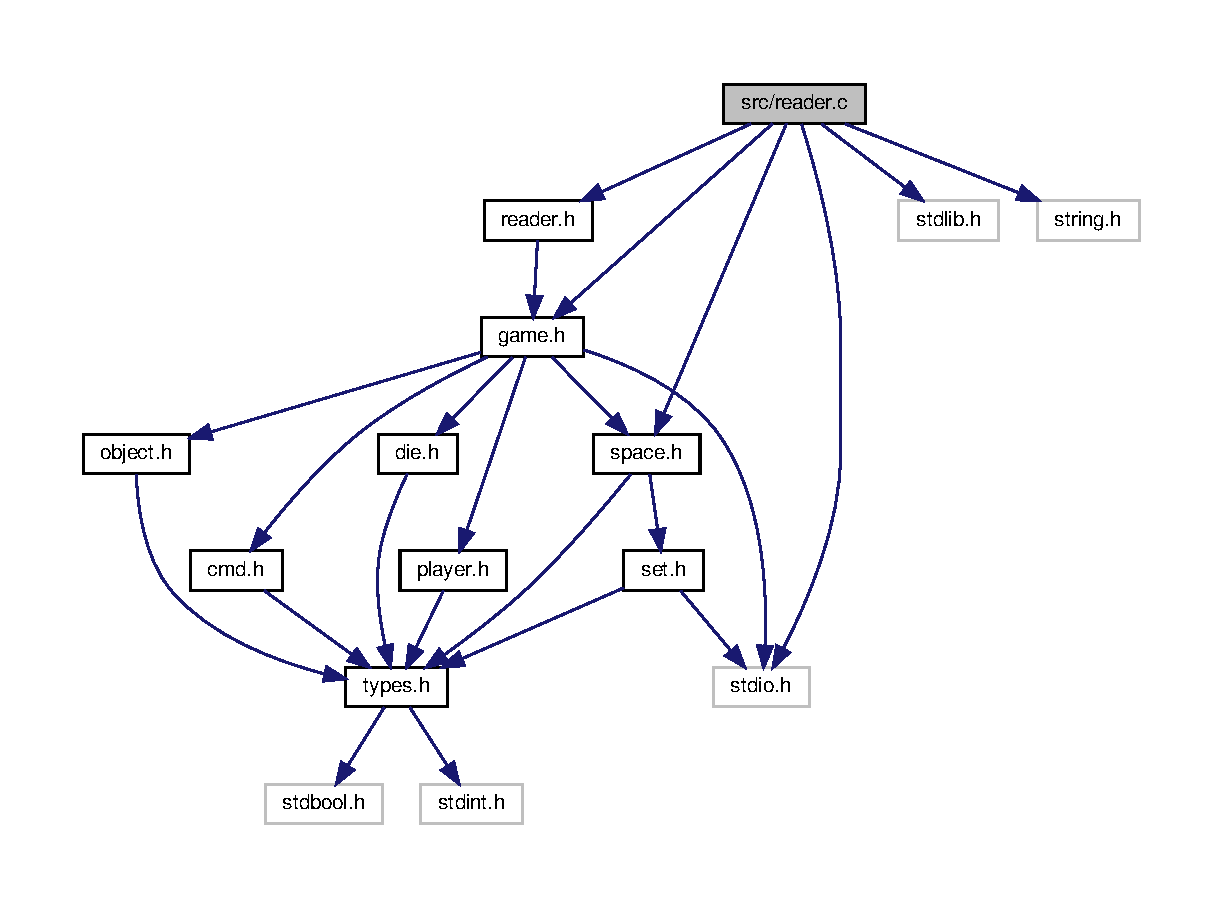
\includegraphics[width=350pt]{reader_8c__incl}
\end{center}
\end{figure}
\subsection*{Functions}
\begin{DoxyCompactItemize}
\item 
S\+T\+A\+T\+US \hyperlink{reader_8c_a329b3f09b9f244887808b807a33457c8}{reader\+\_\+load\+\_\+spaces} (\hyperlink{struct__Game}{Game} $\ast$game, char $\ast$f\+\_\+name)
\begin{DoxyCompactList}\small\item\em Loads spaces from a file. \end{DoxyCompactList}\item 
S\+T\+A\+T\+US \hyperlink{reader_8c_ab8bed1641bb108e505b372bfb23a6604}{reader\+\_\+load\+\_\+objects} (\hyperlink{struct__Game}{Game} $\ast$game, char $\ast$f\+\_\+name)
\begin{DoxyCompactList}\small\item\em Loads objects from a file. \end{DoxyCompactList}\end{DoxyCompactItemize}


\subsection{Detailed Description}
Main game reader. 

The main function of this module is read data from files

\begin{DoxyVersion}{Version}
1.\+0 
\end{DoxyVersion}
\begin{DoxyDate}{Date}
07/02/2019 
\end{DoxyDate}
\begin{DoxyAuthor}{Author}
Álvaro Rodríguez 
\end{DoxyAuthor}
\begin{DoxyCopyright}{Copyright}
G\+NU Public License 
\end{DoxyCopyright}


\subsection{Function Documentation}
\mbox{\Hypertarget{reader_8c_a329b3f09b9f244887808b807a33457c8}\label{reader_8c_a329b3f09b9f244887808b807a33457c8}} 
\index{reader.\+c@{reader.\+c}!reader\+\_\+load\+\_\+spaces@{reader\+\_\+load\+\_\+spaces}}
\index{reader\+\_\+load\+\_\+spaces@{reader\+\_\+load\+\_\+spaces}!reader.\+c@{reader.\+c}}
\subsubsection{\texorpdfstring{reader\+\_\+load\+\_\+spaces()}{reader\_load\_spaces()}}
{\footnotesize\ttfamily S\+T\+A\+T\+US reader\+\_\+load\+\_\+spaces (\begin{DoxyParamCaption}\item[{\hyperlink{struct__Game}{Game} $\ast$}]{game,  }\item[{char $\ast$}]{f\+\_\+name }\end{DoxyParamCaption})}



Loads spaces from a file. 

\begin{DoxyDate}{Date}
07/02/2019 
\end{DoxyDate}
\begin{DoxyAuthor}{Author}
Álvaro Rodríguez
\end{DoxyAuthor}

\begin{DoxyParams}{Parameters}
{\em \{\+Game$\ast$\}} & game -\/ Pointer to game data \\
\hline
{\em \{char$\ast$\}} & filename -\/ name of the source file \\
\hline
\end{DoxyParams}

\begin{DoxyRetVals}{Return values}
{\em \{\+S\+T\+A\+T\+U\+S\}} & -\/ Returns an status \\
\hline
\end{DoxyRetVals}
\mbox{\Hypertarget{reader_8c_ab8bed1641bb108e505b372bfb23a6604}\label{reader_8c_ab8bed1641bb108e505b372bfb23a6604}} 
\index{reader.\+c@{reader.\+c}!reader\+\_\+load\+\_\+objects@{reader\+\_\+load\+\_\+objects}}
\index{reader\+\_\+load\+\_\+objects@{reader\+\_\+load\+\_\+objects}!reader.\+c@{reader.\+c}}
\subsubsection{\texorpdfstring{reader\+\_\+load\+\_\+objects()}{reader\_load\_objects()}}
{\footnotesize\ttfamily S\+T\+A\+T\+US reader\+\_\+load\+\_\+objects (\begin{DoxyParamCaption}\item[{\hyperlink{struct__Game}{Game} $\ast$}]{game,  }\item[{char $\ast$}]{f\+\_\+name }\end{DoxyParamCaption})}



Loads objects from a file. 

\begin{DoxyDate}{Date}
07/02/2019 
\end{DoxyDate}
\begin{DoxyAuthor}{Author}
Álvaro Rodríguez
\end{DoxyAuthor}

\begin{DoxyParams}{Parameters}
{\em \{\+Game$\ast$\}} & game -\/ Pointer to game data  \{char$\ast$\} filename -\/ name of the source file \\
\hline
\end{DoxyParams}

\begin{DoxyRetVals}{Return values}
{\em \{\+S\+T\+A\+T\+U\+S\}} & -\/ Returns an status \\
\hline
\end{DoxyRetVals}

\hypertarget{space_8c}{}\section{src/space.c File Reference}
\label{space_8c}\index{src/space.\+c@{src/space.\+c}}
{\ttfamily \#include \char`\"{}str.\+h\char`\"{}}\newline
{\ttfamily \#include \char`\"{}space.\+h\char`\"{}}\newline
{\ttfamily \#include \char`\"{}types.\+h\char`\"{}}\newline
{\ttfamily \#include \char`\"{}object.\+h\char`\"{}}\newline
{\ttfamily \#include $<$stdio.\+h$>$}\newline
{\ttfamily \#include $<$stdlib.\+h$>$}\newline
{\ttfamily \#include $<$string.\+h$>$}\newline
Include dependency graph for space.\+c\+:\nopagebreak
\begin{figure}[H]
\begin{center}
\leavevmode
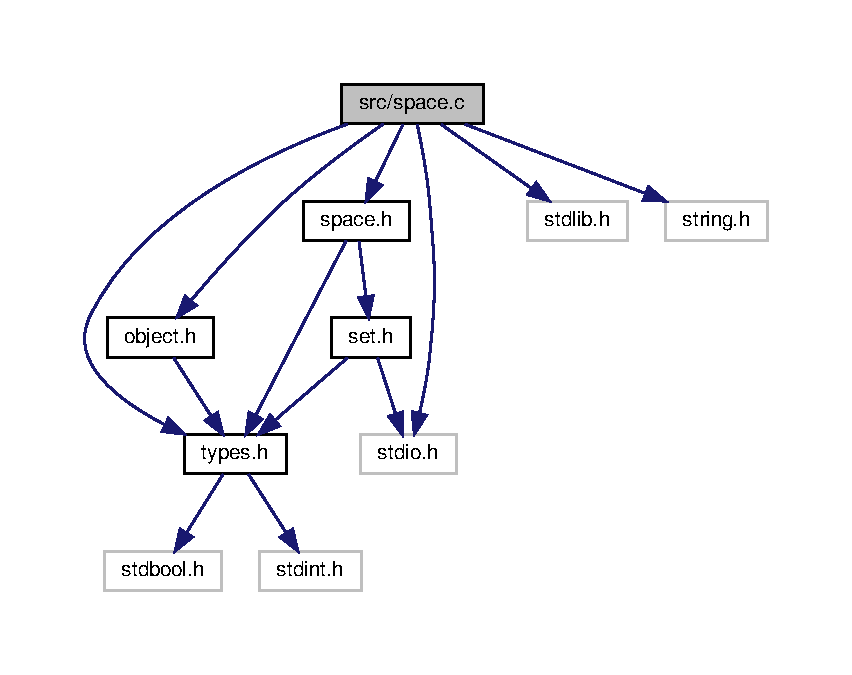
\includegraphics[width=350pt]{space_8c__incl}
\end{center}
\end{figure}
\subsection*{Data Structures}
\begin{DoxyCompactItemize}
\item 
struct \hyperlink{struct__Space}{\+\_\+\+Space}
\begin{DoxyCompactList}\small\item\em Space structure. \end{DoxyCompactList}\end{DoxyCompactItemize}
\subsection*{Functions}
\begin{DoxyCompactItemize}
\item 
\hyperlink{space_8h_a67533ffc2b70463baecc38fb0629bbfc}{Space} $\ast$ \hyperlink{space_8c_a162866fcea156b800fd546d0ffd271c9}{space\+\_\+create} (\hyperlink{types_8h_a845e604fb28f7e3d97549da3448149d3}{Id} id)
\begin{DoxyCompactList}\small\item\em creates a new space \end{DoxyCompactList}\item 
\hyperlink{types_8h_a32c27cc471df37f4fc818d65de0a56c4}{S\+T\+A\+T\+US} \hyperlink{space_8c_a603eff3b1ac49235d9372167b20e2ab9}{space\+\_\+destroy} (\hyperlink{space_8h_a67533ffc2b70463baecc38fb0629bbfc}{Space} $\ast$sp)
\begin{DoxyCompactList}\small\item\em sets to null a space area \end{DoxyCompactList}\item 
\hyperlink{types_8h_a32c27cc471df37f4fc818d65de0a56c4}{S\+T\+A\+T\+US} \hyperlink{space_8c_aab5b468f9822ab78dbe16d1321870d93}{space\+\_\+set\+\_\+name} (\hyperlink{space_8h_a67533ffc2b70463baecc38fb0629bbfc}{Space} $\ast$space, char $\ast$name)
\begin{DoxyCompactList}\small\item\em defines the name of a space \end{DoxyCompactList}\item 
\mbox{\Hypertarget{space_8c_ac81efe6fa2efe470241adc86508c17a2}\label{space_8c_ac81efe6fa2efe470241adc86508c17a2}} 
\hyperlink{types_8h_a32c27cc471df37f4fc818d65de0a56c4}{S\+T\+A\+T\+US} {\bfseries space\+\_\+set\+\_\+picture\+\_\+file} (\hyperlink{space_8h_a67533ffc2b70463baecc38fb0629bbfc}{Space} $\ast$space, char $\ast$f\+\_\+name)
\item 
\hyperlink{types_8h_a32c27cc471df37f4fc818d65de0a56c4}{S\+T\+A\+T\+US} \hyperlink{space_8c_a95f0e95de76db8fa07e8d582c70e1205}{space\+\_\+set\+\_\+descrp} (\hyperlink{space_8h_a67533ffc2b70463baecc38fb0629bbfc}{Space} $\ast$space, const char $\ast$descrp)
\begin{DoxyCompactList}\small\item\em This fuction sets the description of an space. \end{DoxyCompactList}\item 
\hyperlink{types_8h_a32c27cc471df37f4fc818d65de0a56c4}{S\+T\+A\+T\+US} \hyperlink{space_8c_ab287d3c294a9e835e4acc65c44a59057}{space\+\_\+set\+\_\+ldescrp} (\hyperlink{space_8h_a67533ffc2b70463baecc38fb0629bbfc}{Space} $\ast$sp, const char $\ast$ldescrp)
\begin{DoxyCompactList}\small\item\em This fuction sets the long description of an space. \end{DoxyCompactList}\item 
const char $\ast$ \hyperlink{space_8c_a7f830fbc083a277fbe916db402b5bddb}{space\+\_\+get\+\_\+descrp} (\hyperlink{space_8h_a67533ffc2b70463baecc38fb0629bbfc}{Space} $\ast$space)
\begin{DoxyCompactList}\small\item\em This fuction gets the description of an space. \end{DoxyCompactList}\item 
const char $\ast$ \hyperlink{space_8c_aece4b55189d09d85795c112284cd3f91}{space\+\_\+get\+\_\+ldescrp} (\hyperlink{space_8h_a67533ffc2b70463baecc38fb0629bbfc}{Space} $\ast$space)
\begin{DoxyCompactList}\small\item\em This fuction gets the long description of an space. \end{DoxyCompactList}\item 
\mbox{\Hypertarget{space_8c_ab3e618e925fe8ce3b9ff2f04785aed30}\label{space_8c_ab3e618e925fe8ce3b9ff2f04785aed30}} 
const char $\ast$ {\bfseries space\+\_\+get\+\_\+picture\+\_\+file} (\hyperlink{space_8h_a67533ffc2b70463baecc38fb0629bbfc}{Space} $\ast$space)
\item 
\hyperlink{set_8h_a6d3b7f7c92cbb4577ef3ef7ddbf93161}{Set} $\ast$ \hyperlink{space_8c_afc0e3f36d3bdf0105c5d25c256c9cfbd}{space\+\_\+get\+\_\+objects} (\hyperlink{space_8h_a67533ffc2b70463baecc38fb0629bbfc}{Space} $\ast$space)
\begin{DoxyCompactList}\small\item\em This fuction returns the set of objects of the space. \end{DoxyCompactList}\item 
\hyperlink{types_8h_a845e604fb28f7e3d97549da3448149d3}{Id} \hyperlink{space_8c_a753b848210f2098c6328006ae5d90fea}{space\+\_\+get\+\_\+link} (\hyperlink{space_8h_a67533ffc2b70463baecc38fb0629bbfc}{Space} $\ast$sp, \hyperlink{types_8h_a7a09f2d4d51c4b4ba7957bbe676a3855}{Cardinal\+Point} cp)
\begin{DoxyCompactList}\small\item\em Get a link from the space. \end{DoxyCompactList}\item 
\hyperlink{types_8h_a32c27cc471df37f4fc818d65de0a56c4}{S\+T\+A\+T\+US} \hyperlink{space_8c_aba19e670eb78226ebe10c39cf488e72e}{space\+\_\+set\+\_\+link} (\hyperlink{space_8h_a67533ffc2b70463baecc38fb0629bbfc}{Space} $\ast$sp, \hyperlink{types_8h_a7a09f2d4d51c4b4ba7957bbe676a3855}{Cardinal\+Point} cp, \hyperlink{types_8h_a845e604fb28f7e3d97549da3448149d3}{Id} id)
\begin{DoxyCompactList}\small\item\em Sets a links id in a given space. \end{DoxyCompactList}\item 
\hyperlink{types_8h_a32c27cc471df37f4fc818d65de0a56c4}{S\+T\+A\+T\+US} \hyperlink{space_8c_a32c30f0aa89f3f28c06802f1c72c1fdc}{space\+\_\+del\+\_\+object} (\hyperlink{space_8h_a67533ffc2b70463baecc38fb0629bbfc}{Space} $\ast$space, \hyperlink{types_8h_a845e604fb28f7e3d97549da3448149d3}{Id} id)
\begin{DoxyCompactList}\small\item\em it deletes the object with the specified id from the space \end{DoxyCompactList}\item 
bool \hyperlink{space_8c_a3d17d1e189651d3d997891d4649e96c1}{space\+\_\+has\+\_\+object} (\hyperlink{space_8h_a67533ffc2b70463baecc38fb0629bbfc}{Space} $\ast$space, \hyperlink{types_8h_a845e604fb28f7e3d97549da3448149d3}{Id} id)
\begin{DoxyCompactList}\small\item\em checks if the space has an object with the specified id \end{DoxyCompactList}\item 
\hyperlink{types_8h_a32c27cc471df37f4fc818d65de0a56c4}{S\+T\+A\+T\+US} \hyperlink{space_8c_a69b9e22046b7b44dc5aa2afe7cc0a1b9}{space\+\_\+add\+\_\+object} (\hyperlink{space_8h_a67533ffc2b70463baecc38fb0629bbfc}{Space} $\ast$space, \hyperlink{types_8h_a845e604fb28f7e3d97549da3448149d3}{Id} id)
\begin{DoxyCompactList}\small\item\em it adds the object with the specified id to the space \end{DoxyCompactList}\item 
const char $\ast$ \hyperlink{space_8c_a310c540cd6e11073f7328add1f927001}{space\+\_\+get\+\_\+name} (\hyperlink{space_8h_a67533ffc2b70463baecc38fb0629bbfc}{Space} $\ast$space)
\begin{DoxyCompactList}\small\item\em takes the name of a space \end{DoxyCompactList}\item 
\hyperlink{types_8h_a845e604fb28f7e3d97549da3448149d3}{Id} \hyperlink{space_8c_ac8ddfd0d8692fd852ee49698c446cb50}{space\+\_\+get\+\_\+id} (\hyperlink{space_8h_a67533ffc2b70463baecc38fb0629bbfc}{Space} $\ast$space)
\begin{DoxyCompactList}\small\item\em takes the id of a space \end{DoxyCompactList}\item 
\hyperlink{types_8h_a845e604fb28f7e3d97549da3448149d3}{Id} \hyperlink{space_8c_ab7442e9184cd345333916b04165ab843}{space\+\_\+get\+\_\+object} (\hyperlink{space_8h_a67533ffc2b70463baecc38fb0629bbfc}{Space} $\ast$space, \hyperlink{types_8h_a845e604fb28f7e3d97549da3448149d3}{Id} id)
\begin{DoxyCompactList}\small\item\em gets a pointer towads an object \end{DoxyCompactList}\item 
\hyperlink{types_8h_a32c27cc471df37f4fc818d65de0a56c4}{S\+T\+A\+T\+US} \hyperlink{space_8c_a49badcee7e68b79f40dad37c83193f74}{space\+\_\+set\+\_\+picture} (\hyperlink{space_8h_a67533ffc2b70463baecc38fb0629bbfc}{Space} $\ast$space, char $\ast$pict)
\begin{DoxyCompactList}\small\item\em it paints the figure associated to the space \end{DoxyCompactList}\item 
char $\ast$ \hyperlink{space_8c_ae1afecfe9f7bb189edfc2f5bbd39b47f}{space\+\_\+get\+\_\+picture} (\hyperlink{space_8h_a67533ffc2b70463baecc38fb0629bbfc}{Space} $\ast$space)
\begin{DoxyCompactList}\small\item\em it gets the figure associated to the specified space \end{DoxyCompactList}\item 
\hyperlink{types_8h_a32c27cc471df37f4fc818d65de0a56c4}{S\+T\+A\+T\+US} \hyperlink{space_8c_a592c8caf308e1dd0940bda10e96d7307}{space\+\_\+set\+\_\+light} (\hyperlink{space_8h_a67533ffc2b70463baecc38fb0629bbfc}{Space} $\ast$space, bool l)
\begin{DoxyCompactList}\small\item\em Sets a light in a given space. \end{DoxyCompactList}\item 
\hyperlink{types_8h_a32c27cc471df37f4fc818d65de0a56c4}{S\+T\+A\+T\+US} \hyperlink{space_8c_a354a9e08bd0097e2c027a2d44bb4bdf4}{space\+\_\+toggle\+\_\+light} (\hyperlink{space_8h_a67533ffc2b70463baecc38fb0629bbfc}{Space} $\ast$space)
\begin{DoxyCompactList}\small\item\em Toggles the light of a given space. \end{DoxyCompactList}\item 
bool \hyperlink{space_8c_a4000018f7cb697532dd7cffc2c36f72f}{space\+\_\+get\+\_\+light} (\hyperlink{space_8h_a67533ffc2b70463baecc38fb0629bbfc}{Space} $\ast$space)
\begin{DoxyCompactList}\small\item\em Gets the light status of a given space. \end{DoxyCompactList}\item 
int \hyperlink{space_8c_a845ef83c595c94bd1224f6563efebf34}{space\+\_\+print} (\hyperlink{space_8h_a67533ffc2b70463baecc38fb0629bbfc}{Space} $\ast$space)
\begin{DoxyCompactList}\small\item\em prints a space \end{DoxyCompactList}\end{DoxyCompactItemize}


\subsection{Detailed Description}
Manages the cells player can move to.

\begin{DoxyVersion}{Version}
1.\+0 
\end{DoxyVersion}
\begin{DoxyDate}{Date}
07/02/2019 
\end{DoxyDate}
\begin{DoxyCopyright}{Copyright}
G\+NU Public License 
\end{DoxyCopyright}


\subsection{Function Documentation}
\mbox{\Hypertarget{space_8c_a162866fcea156b800fd546d0ffd271c9}\label{space_8c_a162866fcea156b800fd546d0ffd271c9}} 
\index{space.\+c@{space.\+c}!space\+\_\+create@{space\+\_\+create}}
\index{space\+\_\+create@{space\+\_\+create}!space.\+c@{space.\+c}}
\subsubsection{\texorpdfstring{space\+\_\+create()}{space\_create()}}
{\footnotesize\ttfamily \hyperlink{space_8h_a67533ffc2b70463baecc38fb0629bbfc}{Space}$\ast$ space\+\_\+create (\begin{DoxyParamCaption}\item[{\hyperlink{types_8h_a845e604fb28f7e3d97549da3448149d3}{Id}}]{id }\end{DoxyParamCaption})}



creates a new space 

\begin{DoxyAuthor}{Author}
Javier Romera 
\end{DoxyAuthor}

\begin{DoxyParams}{Parameters}
{\em \{\+Id\}} & -\/ Space identification \\
\hline
\end{DoxyParams}

\begin{DoxyRetVals}{Return values}
{\em \{\+Space$\ast$\}} & -\/ returns an space pointer \\
\hline
\end{DoxyRetVals}
\mbox{\Hypertarget{space_8c_a603eff3b1ac49235d9372167b20e2ab9}\label{space_8c_a603eff3b1ac49235d9372167b20e2ab9}} 
\index{space.\+c@{space.\+c}!space\+\_\+destroy@{space\+\_\+destroy}}
\index{space\+\_\+destroy@{space\+\_\+destroy}!space.\+c@{space.\+c}}
\subsubsection{\texorpdfstring{space\+\_\+destroy()}{space\_destroy()}}
{\footnotesize\ttfamily \hyperlink{types_8h_a32c27cc471df37f4fc818d65de0a56c4}{S\+T\+A\+T\+US} space\+\_\+destroy (\begin{DoxyParamCaption}\item[{\hyperlink{space_8h_a67533ffc2b70463baecc38fb0629bbfc}{Space} $\ast$}]{space }\end{DoxyParamCaption})}



sets to null a space area 

\begin{DoxyAuthor}{Author}
Javier Romera 
\end{DoxyAuthor}
\begin{DoxyVersion}{Version}
2.\+0 
\end{DoxyVersion}

\begin{DoxyParams}{Parameters}
{\em \{\+Space$\ast$\}} & space -\/ Space pointer \\
\hline
\end{DoxyParams}

\begin{DoxyRetVals}{Return values}
{\em \{\+S\+T\+A\+T\+U\+S\}} & -\/ Returns a state \\
\hline
\end{DoxyRetVals}
\mbox{\Hypertarget{space_8c_aab5b468f9822ab78dbe16d1321870d93}\label{space_8c_aab5b468f9822ab78dbe16d1321870d93}} 
\index{space.\+c@{space.\+c}!space\+\_\+set\+\_\+name@{space\+\_\+set\+\_\+name}}
\index{space\+\_\+set\+\_\+name@{space\+\_\+set\+\_\+name}!space.\+c@{space.\+c}}
\subsubsection{\texorpdfstring{space\+\_\+set\+\_\+name()}{space\_set\_name()}}
{\footnotesize\ttfamily \hyperlink{types_8h_a32c27cc471df37f4fc818d65de0a56c4}{S\+T\+A\+T\+US} space\+\_\+set\+\_\+name (\begin{DoxyParamCaption}\item[{\hyperlink{space_8h_a67533ffc2b70463baecc38fb0629bbfc}{Space} $\ast$}]{space,  }\item[{char $\ast$}]{name }\end{DoxyParamCaption})}



defines the name of a space 

\begin{DoxyAuthor}{Author}
Javier Romera 
\end{DoxyAuthor}

\begin{DoxyParams}{Parameters}
{\em \{\+Space$\ast$\}} & -\/ space \\
\hline
{\em \{\+Char$\ast$\}} & -\/ name \\
\hline
\end{DoxyParams}

\begin{DoxyRetVals}{Return values}
{\em \{\+S\+T\+A\+T\+U\+S\}} & -\/ Returns an state \\
\hline
\end{DoxyRetVals}
\mbox{\Hypertarget{space_8c_a95f0e95de76db8fa07e8d582c70e1205}\label{space_8c_a95f0e95de76db8fa07e8d582c70e1205}} 
\index{space.\+c@{space.\+c}!space\+\_\+set\+\_\+descrp@{space\+\_\+set\+\_\+descrp}}
\index{space\+\_\+set\+\_\+descrp@{space\+\_\+set\+\_\+descrp}!space.\+c@{space.\+c}}
\subsubsection{\texorpdfstring{space\+\_\+set\+\_\+descrp()}{space\_set\_descrp()}}
{\footnotesize\ttfamily \hyperlink{types_8h_a32c27cc471df37f4fc818d65de0a56c4}{S\+T\+A\+T\+US} space\+\_\+set\+\_\+descrp (\begin{DoxyParamCaption}\item[{\hyperlink{space_8h_a67533ffc2b70463baecc38fb0629bbfc}{Space} $\ast$}]{space,  }\item[{const char $\ast$}]{descrp }\end{DoxyParamCaption})}



This fuction sets the description of an space. 

\begin{DoxyAuthor}{Author}
Javier Romera 
\end{DoxyAuthor}

\begin{DoxyParams}{Parameters}
{\em \{\+Space$\ast$\}} & obj -\/ space\textquotesingle{}s pointer \\
\hline
{\em \{char$\ast$\}} & descrp -\/ short description of the space \\
\hline
\end{DoxyParams}

\begin{DoxyRetVals}{Return values}
{\em \{\+S\+T\+A\+T\+U\+S\}} & -\/ Returns status code \\
\hline
\end{DoxyRetVals}
\mbox{\Hypertarget{space_8c_ab287d3c294a9e835e4acc65c44a59057}\label{space_8c_ab287d3c294a9e835e4acc65c44a59057}} 
\index{space.\+c@{space.\+c}!space\+\_\+set\+\_\+ldescrp@{space\+\_\+set\+\_\+ldescrp}}
\index{space\+\_\+set\+\_\+ldescrp@{space\+\_\+set\+\_\+ldescrp}!space.\+c@{space.\+c}}
\subsubsection{\texorpdfstring{space\+\_\+set\+\_\+ldescrp()}{space\_set\_ldescrp()}}
{\footnotesize\ttfamily \hyperlink{types_8h_a32c27cc471df37f4fc818d65de0a56c4}{S\+T\+A\+T\+US} space\+\_\+set\+\_\+ldescrp (\begin{DoxyParamCaption}\item[{\hyperlink{space_8h_a67533ffc2b70463baecc38fb0629bbfc}{Space} $\ast$}]{space,  }\item[{const char $\ast$}]{ldescrp }\end{DoxyParamCaption})}



This fuction sets the long description of an space. 

\begin{DoxyAuthor}{Author}
Javier Romera 
\end{DoxyAuthor}

\begin{DoxyParams}{Parameters}
{\em \{\+Space$\ast$\}} & obj -\/ space\textquotesingle{}s pointer \\
\hline
{\em \{char$\ast$\}} & ldescrp -\/ long description of the space \\
\hline
\end{DoxyParams}

\begin{DoxyRetVals}{Return values}
{\em \{\+S\+T\+A\+T\+U\+S\}} & -\/ Returns status code \\
\hline
\end{DoxyRetVals}
\mbox{\Hypertarget{space_8c_a7f830fbc083a277fbe916db402b5bddb}\label{space_8c_a7f830fbc083a277fbe916db402b5bddb}} 
\index{space.\+c@{space.\+c}!space\+\_\+get\+\_\+descrp@{space\+\_\+get\+\_\+descrp}}
\index{space\+\_\+get\+\_\+descrp@{space\+\_\+get\+\_\+descrp}!space.\+c@{space.\+c}}
\subsubsection{\texorpdfstring{space\+\_\+get\+\_\+descrp()}{space\_get\_descrp()}}
{\footnotesize\ttfamily const char$\ast$ space\+\_\+get\+\_\+descrp (\begin{DoxyParamCaption}\item[{\hyperlink{space_8h_a67533ffc2b70463baecc38fb0629bbfc}{Space} $\ast$}]{space }\end{DoxyParamCaption})}



This fuction gets the description of an space. 

\begin{DoxyAuthor}{Author}
Javier Romera 
\end{DoxyAuthor}

\begin{DoxyParams}{Parameters}
{\em \{\+Space$\ast$\}} & obj -\/ space\textquotesingle{}s pointer \\
\hline
\end{DoxyParams}

\begin{DoxyRetVals}{Return values}
{\em \{char$\ast$\}} & -\/ Returns the space name \\
\hline
\end{DoxyRetVals}
\mbox{\Hypertarget{space_8c_aece4b55189d09d85795c112284cd3f91}\label{space_8c_aece4b55189d09d85795c112284cd3f91}} 
\index{space.\+c@{space.\+c}!space\+\_\+get\+\_\+ldescrp@{space\+\_\+get\+\_\+ldescrp}}
\index{space\+\_\+get\+\_\+ldescrp@{space\+\_\+get\+\_\+ldescrp}!space.\+c@{space.\+c}}
\subsubsection{\texorpdfstring{space\+\_\+get\+\_\+ldescrp()}{space\_get\_ldescrp()}}
{\footnotesize\ttfamily const char$\ast$ space\+\_\+get\+\_\+ldescrp (\begin{DoxyParamCaption}\item[{\hyperlink{space_8h_a67533ffc2b70463baecc38fb0629bbfc}{Space} $\ast$}]{space }\end{DoxyParamCaption})}



This fuction gets the long description of an space. 

\begin{DoxyAuthor}{Author}
Javier Romera 
\end{DoxyAuthor}

\begin{DoxyParams}{Parameters}
{\em \{\+Space$\ast$\}} & obj -\/ space\textquotesingle{}s pointer \\
\hline
\end{DoxyParams}

\begin{DoxyRetVals}{Return values}
{\em \{char$\ast$\}} & -\/ Returns a long description of the space \\
\hline
\end{DoxyRetVals}
\mbox{\Hypertarget{space_8c_afc0e3f36d3bdf0105c5d25c256c9cfbd}\label{space_8c_afc0e3f36d3bdf0105c5d25c256c9cfbd}} 
\index{space.\+c@{space.\+c}!space\+\_\+get\+\_\+objects@{space\+\_\+get\+\_\+objects}}
\index{space\+\_\+get\+\_\+objects@{space\+\_\+get\+\_\+objects}!space.\+c@{space.\+c}}
\subsubsection{\texorpdfstring{space\+\_\+get\+\_\+objects()}{space\_get\_objects()}}
{\footnotesize\ttfamily \hyperlink{set_8h_a6d3b7f7c92cbb4577ef3ef7ddbf93161}{Set}$\ast$ space\+\_\+get\+\_\+objects (\begin{DoxyParamCaption}\item[{\hyperlink{space_8h_a67533ffc2b70463baecc38fb0629bbfc}{Space} $\ast$}]{space }\end{DoxyParamCaption})}



This fuction returns the set of objects of the space. 

\begin{DoxyAuthor}{Author}
Javier Romera 
\end{DoxyAuthor}

\begin{DoxyParams}{Parameters}
{\em \{\+Space$\ast$\}} & obj -\/ space\textquotesingle{}s pointer \\
\hline
\end{DoxyParams}

\begin{DoxyRetVals}{Return values}
{\em \{\+Space$\ast$\}} & -\/ Set of objects \\
\hline
\end{DoxyRetVals}
\mbox{\Hypertarget{space_8c_a753b848210f2098c6328006ae5d90fea}\label{space_8c_a753b848210f2098c6328006ae5d90fea}} 
\index{space.\+c@{space.\+c}!space\+\_\+get\+\_\+link@{space\+\_\+get\+\_\+link}}
\index{space\+\_\+get\+\_\+link@{space\+\_\+get\+\_\+link}!space.\+c@{space.\+c}}
\subsubsection{\texorpdfstring{space\+\_\+get\+\_\+link()}{space\_get\_link()}}
{\footnotesize\ttfamily \hyperlink{types_8h_a845e604fb28f7e3d97549da3448149d3}{Id} space\+\_\+get\+\_\+link (\begin{DoxyParamCaption}\item[{\hyperlink{space_8h_a67533ffc2b70463baecc38fb0629bbfc}{Space} $\ast$}]{sp,  }\item[{\hyperlink{types_8h_a7a09f2d4d51c4b4ba7957bbe676a3855}{Cardinal\+Point}}]{cp }\end{DoxyParamCaption})}



Get a link from the space. 


\begin{DoxyParams}{Parameters}
{\em \{\+Sapce$\ast$\}} & sp -\/ Space pointer \\
\hline
{\em \{\+Cardinal\+Point\}} & cp -\/ Cardinal point of the space \\
\hline
\end{DoxyParams}
\mbox{\Hypertarget{space_8c_aba19e670eb78226ebe10c39cf488e72e}\label{space_8c_aba19e670eb78226ebe10c39cf488e72e}} 
\index{space.\+c@{space.\+c}!space\+\_\+set\+\_\+link@{space\+\_\+set\+\_\+link}}
\index{space\+\_\+set\+\_\+link@{space\+\_\+set\+\_\+link}!space.\+c@{space.\+c}}
\subsubsection{\texorpdfstring{space\+\_\+set\+\_\+link()}{space\_set\_link()}}
{\footnotesize\ttfamily \hyperlink{types_8h_a32c27cc471df37f4fc818d65de0a56c4}{S\+T\+A\+T\+US} space\+\_\+set\+\_\+link (\begin{DoxyParamCaption}\item[{\hyperlink{space_8h_a67533ffc2b70463baecc38fb0629bbfc}{Space} $\ast$}]{sp,  }\item[{\hyperlink{types_8h_a7a09f2d4d51c4b4ba7957bbe676a3855}{Cardinal\+Point}}]{cp,  }\item[{\hyperlink{types_8h_a845e604fb28f7e3d97549da3448149d3}{Id}}]{id }\end{DoxyParamCaption})}



Sets a links id in a given space. 


\begin{DoxyParams}{Parameters}
{\em \{\+Sapce$\ast$\}} & sp -\/ Space pointer \\
\hline
{\em \{\+Cardinal\+Point\}} & cp -\/ Cardinal point of the space \\
\hline
{\em \{\+Id\}} & id -\/ Link\textquotesingle{}s id \\
\hline
\end{DoxyParams}

\begin{DoxyRetVals}{Return values}
{\em \{\+S\+T\+A\+T\+U\+S\}} & -\/ Returns an status \\
\hline
\end{DoxyRetVals}
\mbox{\Hypertarget{space_8c_a32c30f0aa89f3f28c06802f1c72c1fdc}\label{space_8c_a32c30f0aa89f3f28c06802f1c72c1fdc}} 
\index{space.\+c@{space.\+c}!space\+\_\+del\+\_\+object@{space\+\_\+del\+\_\+object}}
\index{space\+\_\+del\+\_\+object@{space\+\_\+del\+\_\+object}!space.\+c@{space.\+c}}
\subsubsection{\texorpdfstring{space\+\_\+del\+\_\+object()}{space\_del\_object()}}
{\footnotesize\ttfamily \hyperlink{types_8h_a32c27cc471df37f4fc818d65de0a56c4}{S\+T\+A\+T\+US} space\+\_\+del\+\_\+object (\begin{DoxyParamCaption}\item[{\hyperlink{space_8h_a67533ffc2b70463baecc38fb0629bbfc}{Space} $\ast$}]{space,  }\item[{\hyperlink{types_8h_a845e604fb28f7e3d97549da3448149d3}{Id}}]{id }\end{DoxyParamCaption})}



it deletes the object with the specified id from the space 

\begin{DoxyAuthor}{Author}
Javier Romera 
\end{DoxyAuthor}

\begin{DoxyParams}{Parameters}
{\em \{\+Space$\ast$\}} & -\/ space \\
\hline
{\em \{\+Id\}} & -\/ id \\
\hline
\end{DoxyParams}

\begin{DoxyRetVals}{Return values}
{\em \{\+S\+T\+A\+T\+U\+S\}} & -\/ Returns an state \\
\hline
\end{DoxyRetVals}
\mbox{\Hypertarget{space_8c_a3d17d1e189651d3d997891d4649e96c1}\label{space_8c_a3d17d1e189651d3d997891d4649e96c1}} 
\index{space.\+c@{space.\+c}!space\+\_\+has\+\_\+object@{space\+\_\+has\+\_\+object}}
\index{space\+\_\+has\+\_\+object@{space\+\_\+has\+\_\+object}!space.\+c@{space.\+c}}
\subsubsection{\texorpdfstring{space\+\_\+has\+\_\+object()}{space\_has\_object()}}
{\footnotesize\ttfamily bool space\+\_\+has\+\_\+object (\begin{DoxyParamCaption}\item[{\hyperlink{space_8h_a67533ffc2b70463baecc38fb0629bbfc}{Space} $\ast$}]{space,  }\item[{\hyperlink{types_8h_a845e604fb28f7e3d97549da3448149d3}{Id}}]{id }\end{DoxyParamCaption})}



checks if the space has an object with the specified id 

\begin{DoxyAuthor}{Author}
Javier Romera 
\end{DoxyAuthor}

\begin{DoxyParams}{Parameters}
{\em \{\+Space\}} & -\/ space \\
\hline
{\em \{\+Id\}} & -\/ id \\
\hline
\end{DoxyParams}

\begin{DoxyRetVals}{Return values}
{\em \{bool\}} & -\/ Returns T\+R\+UE or F\+A\+L\+SE \\
\hline
\end{DoxyRetVals}
\mbox{\Hypertarget{space_8c_a69b9e22046b7b44dc5aa2afe7cc0a1b9}\label{space_8c_a69b9e22046b7b44dc5aa2afe7cc0a1b9}} 
\index{space.\+c@{space.\+c}!space\+\_\+add\+\_\+object@{space\+\_\+add\+\_\+object}}
\index{space\+\_\+add\+\_\+object@{space\+\_\+add\+\_\+object}!space.\+c@{space.\+c}}
\subsubsection{\texorpdfstring{space\+\_\+add\+\_\+object()}{space\_add\_object()}}
{\footnotesize\ttfamily \hyperlink{types_8h_a32c27cc471df37f4fc818d65de0a56c4}{S\+T\+A\+T\+US} space\+\_\+add\+\_\+object (\begin{DoxyParamCaption}\item[{\hyperlink{space_8h_a67533ffc2b70463baecc38fb0629bbfc}{Space} $\ast$}]{space,  }\item[{\hyperlink{types_8h_a845e604fb28f7e3d97549da3448149d3}{Id}}]{id }\end{DoxyParamCaption})}



it adds the object with the specified id to the space 

\begin{DoxyAuthor}{Author}
Javier Romera 
\end{DoxyAuthor}

\begin{DoxyParams}{Parameters}
{\em \{\+Space$\ast$\}} & -\/ space \\
\hline
{\em \{\+Id\}} & -\/ id \\
\hline
\end{DoxyParams}

\begin{DoxyRetVals}{Return values}
{\em \{\+S\+T\+A\+T\+U\+S\}} & -\/ Returns an state \\
\hline
\end{DoxyRetVals}
\mbox{\Hypertarget{space_8c_a310c540cd6e11073f7328add1f927001}\label{space_8c_a310c540cd6e11073f7328add1f927001}} 
\index{space.\+c@{space.\+c}!space\+\_\+get\+\_\+name@{space\+\_\+get\+\_\+name}}
\index{space\+\_\+get\+\_\+name@{space\+\_\+get\+\_\+name}!space.\+c@{space.\+c}}
\subsubsection{\texorpdfstring{space\+\_\+get\+\_\+name()}{space\_get\_name()}}
{\footnotesize\ttfamily const char$\ast$ space\+\_\+get\+\_\+name (\begin{DoxyParamCaption}\item[{\hyperlink{space_8h_a67533ffc2b70463baecc38fb0629bbfc}{Space} $\ast$}]{space }\end{DoxyParamCaption})}



takes the name of a space 

\begin{DoxyAuthor}{Author}
Javier Romera 
\end{DoxyAuthor}
\begin{DoxyVersion}{Version}
2.\+0 
\end{DoxyVersion}
\begin{DoxyDate}{Date}
07/02/2019 
\end{DoxyDate}

\begin{DoxyParams}{Parameters}
{\em \{\+Space$\ast$\}} & -\/ space \\
\hline
\end{DoxyParams}

\begin{DoxyRetVals}{Return values}
{\em \{char$\ast$\}} & -\/ Returns an array of characters \\
\hline
\end{DoxyRetVals}
\mbox{\Hypertarget{space_8c_ac8ddfd0d8692fd852ee49698c446cb50}\label{space_8c_ac8ddfd0d8692fd852ee49698c446cb50}} 
\index{space.\+c@{space.\+c}!space\+\_\+get\+\_\+id@{space\+\_\+get\+\_\+id}}
\index{space\+\_\+get\+\_\+id@{space\+\_\+get\+\_\+id}!space.\+c@{space.\+c}}
\subsubsection{\texorpdfstring{space\+\_\+get\+\_\+id()}{space\_get\_id()}}
{\footnotesize\ttfamily \hyperlink{types_8h_a845e604fb28f7e3d97549da3448149d3}{Id} space\+\_\+get\+\_\+id (\begin{DoxyParamCaption}\item[{\hyperlink{space_8h_a67533ffc2b70463baecc38fb0629bbfc}{Space} $\ast$}]{space }\end{DoxyParamCaption})}



takes the id of a space 

\begin{DoxyAuthor}{Author}
Javier Romera 
\end{DoxyAuthor}
\begin{DoxyVersion}{Version}
2.\+0 
\end{DoxyVersion}

\begin{DoxyParams}{Parameters}
{\em \{\+Space$\ast$\}} & space -\/ Space pointer \\
\hline
\end{DoxyParams}

\begin{DoxyRetVals}{Return values}
{\em \{\+Id\}} & -\/ Returns an id \\
\hline
\end{DoxyRetVals}
\mbox{\Hypertarget{space_8c_ab7442e9184cd345333916b04165ab843}\label{space_8c_ab7442e9184cd345333916b04165ab843}} 
\index{space.\+c@{space.\+c}!space\+\_\+get\+\_\+object@{space\+\_\+get\+\_\+object}}
\index{space\+\_\+get\+\_\+object@{space\+\_\+get\+\_\+object}!space.\+c@{space.\+c}}
\subsubsection{\texorpdfstring{space\+\_\+get\+\_\+object()}{space\_get\_object()}}
{\footnotesize\ttfamily \hyperlink{types_8h_a845e604fb28f7e3d97549da3448149d3}{Id} space\+\_\+get\+\_\+object (\begin{DoxyParamCaption}\item[{\hyperlink{space_8h_a67533ffc2b70463baecc38fb0629bbfc}{Space} $\ast$}]{space,  }\item[{\hyperlink{types_8h_a845e604fb28f7e3d97549da3448149d3}{Id}}]{id }\end{DoxyParamCaption})}



gets a pointer towads an object 

\begin{DoxyAuthor}{Author}
Javier Romera 
\end{DoxyAuthor}

\begin{DoxyParams}{Parameters}
{\em \{\+Game$\ast$\}} & -\/ game \\
\hline
\end{DoxyParams}
\mbox{\Hypertarget{space_8c_a49badcee7e68b79f40dad37c83193f74}\label{space_8c_a49badcee7e68b79f40dad37c83193f74}} 
\index{space.\+c@{space.\+c}!space\+\_\+set\+\_\+picture@{space\+\_\+set\+\_\+picture}}
\index{space\+\_\+set\+\_\+picture@{space\+\_\+set\+\_\+picture}!space.\+c@{space.\+c}}
\subsubsection{\texorpdfstring{space\+\_\+set\+\_\+picture()}{space\_set\_picture()}}
{\footnotesize\ttfamily \hyperlink{types_8h_a32c27cc471df37f4fc818d65de0a56c4}{S\+T\+A\+T\+US} space\+\_\+set\+\_\+picture (\begin{DoxyParamCaption}\item[{\hyperlink{space_8h_a67533ffc2b70463baecc38fb0629bbfc}{Space} $\ast$}]{space,  }\item[{char $\ast$}]{pict }\end{DoxyParamCaption})}



it paints the figure associated to the space 

\begin{DoxyAuthor}{Author}
Javier Romera 
\end{DoxyAuthor}

\begin{DoxyParams}{Parameters}
{\em \{\+Space$\ast$\}} & -\/ space \\
\hline
{\em \{char$\ast$\}} & -\/ pict \\
\hline
\end{DoxyParams}

\begin{DoxyRetVals}{Return values}
{\em \{\+S\+T\+A\+T\+U\+S\}} & -\/ Returns an state \\
\hline
\end{DoxyRetVals}
\mbox{\Hypertarget{space_8c_ae1afecfe9f7bb189edfc2f5bbd39b47f}\label{space_8c_ae1afecfe9f7bb189edfc2f5bbd39b47f}} 
\index{space.\+c@{space.\+c}!space\+\_\+get\+\_\+picture@{space\+\_\+get\+\_\+picture}}
\index{space\+\_\+get\+\_\+picture@{space\+\_\+get\+\_\+picture}!space.\+c@{space.\+c}}
\subsubsection{\texorpdfstring{space\+\_\+get\+\_\+picture()}{space\_get\_picture()}}
{\footnotesize\ttfamily char$\ast$ space\+\_\+get\+\_\+picture (\begin{DoxyParamCaption}\item[{\hyperlink{space_8h_a67533ffc2b70463baecc38fb0629bbfc}{Space} $\ast$}]{space }\end{DoxyParamCaption})}



it gets the figure associated to the specified space 

\begin{DoxyAuthor}{Author}
Javier Romera 
\end{DoxyAuthor}

\begin{DoxyParams}{Parameters}
{\em \{\+Space$\ast$\}} & -\/ space \\
\hline
\end{DoxyParams}

\begin{DoxyRetVals}{Return values}
{\em \{char$\ast$\}} & -\/ Returns a pointer to char \\
\hline
\end{DoxyRetVals}
\mbox{\Hypertarget{space_8c_a592c8caf308e1dd0940bda10e96d7307}\label{space_8c_a592c8caf308e1dd0940bda10e96d7307}} 
\index{space.\+c@{space.\+c}!space\+\_\+set\+\_\+light@{space\+\_\+set\+\_\+light}}
\index{space\+\_\+set\+\_\+light@{space\+\_\+set\+\_\+light}!space.\+c@{space.\+c}}
\subsubsection{\texorpdfstring{space\+\_\+set\+\_\+light()}{space\_set\_light()}}
{\footnotesize\ttfamily \hyperlink{types_8h_a32c27cc471df37f4fc818d65de0a56c4}{S\+T\+A\+T\+US} space\+\_\+set\+\_\+light (\begin{DoxyParamCaption}\item[{\hyperlink{space_8h_a67533ffc2b70463baecc38fb0629bbfc}{Space} $\ast$}]{space,  }\item[{bool}]{l }\end{DoxyParamCaption})}



Sets a light in a given space. 


\begin{DoxyParams}{Parameters}
{\em \{\+Sapce$\ast$\}} & space -\/ Space pointer \\
\hline
{\em \{bool\}} & l -\/ light of the space \\
\hline
\end{DoxyParams}

\begin{DoxyRetVals}{Return values}
{\em \{\+S\+T\+A\+T\+U\+S\}} & -\/ Returns an status \\
\hline
\end{DoxyRetVals}
\mbox{\Hypertarget{space_8c_a354a9e08bd0097e2c027a2d44bb4bdf4}\label{space_8c_a354a9e08bd0097e2c027a2d44bb4bdf4}} 
\index{space.\+c@{space.\+c}!space\+\_\+toggle\+\_\+light@{space\+\_\+toggle\+\_\+light}}
\index{space\+\_\+toggle\+\_\+light@{space\+\_\+toggle\+\_\+light}!space.\+c@{space.\+c}}
\subsubsection{\texorpdfstring{space\+\_\+toggle\+\_\+light()}{space\_toggle\_light()}}
{\footnotesize\ttfamily \hyperlink{types_8h_a32c27cc471df37f4fc818d65de0a56c4}{S\+T\+A\+T\+US} space\+\_\+toggle\+\_\+light (\begin{DoxyParamCaption}\item[{\hyperlink{space_8h_a67533ffc2b70463baecc38fb0629bbfc}{Space} $\ast$}]{space }\end{DoxyParamCaption})}



Toggles the light of a given space. 


\begin{DoxyParams}{Parameters}
{\em \{\+Sapce$\ast$\}} & space -\/ Space pointer \\
\hline
\end{DoxyParams}

\begin{DoxyRetVals}{Return values}
{\em \{\+S\+T\+A\+T\+U\+S\}} & -\/ Returns a status code \\
\hline
\end{DoxyRetVals}
\mbox{\Hypertarget{space_8c_a4000018f7cb697532dd7cffc2c36f72f}\label{space_8c_a4000018f7cb697532dd7cffc2c36f72f}} 
\index{space.\+c@{space.\+c}!space\+\_\+get\+\_\+light@{space\+\_\+get\+\_\+light}}
\index{space\+\_\+get\+\_\+light@{space\+\_\+get\+\_\+light}!space.\+c@{space.\+c}}
\subsubsection{\texorpdfstring{space\+\_\+get\+\_\+light()}{space\_get\_light()}}
{\footnotesize\ttfamily bool space\+\_\+get\+\_\+light (\begin{DoxyParamCaption}\item[{\hyperlink{space_8h_a67533ffc2b70463baecc38fb0629bbfc}{Space} $\ast$}]{space }\end{DoxyParamCaption})}



Gets the light status of a given space. 


\begin{DoxyParams}{Parameters}
{\em \{\+Sapce$\ast$\}} & space -\/ Space pointer \\
\hline
\end{DoxyParams}

\begin{DoxyRetVals}{Return values}
{\em \{\+S\+T\+A\+T\+U\+S\}} & -\/ Returns a boolean value \\
\hline
\end{DoxyRetVals}
\mbox{\Hypertarget{space_8c_a845ef83c595c94bd1224f6563efebf34}\label{space_8c_a845ef83c595c94bd1224f6563efebf34}} 
\index{space.\+c@{space.\+c}!space\+\_\+print@{space\+\_\+print}}
\index{space\+\_\+print@{space\+\_\+print}!space.\+c@{space.\+c}}
\subsubsection{\texorpdfstring{space\+\_\+print()}{space\_print()}}
{\footnotesize\ttfamily int space\+\_\+print (\begin{DoxyParamCaption}\item[{\hyperlink{space_8h_a67533ffc2b70463baecc38fb0629bbfc}{Space} $\ast$}]{space }\end{DoxyParamCaption})}



prints a space 

\begin{DoxyAuthor}{Author}
Javier Romera 
\end{DoxyAuthor}

\begin{DoxyParams}{Parameters}
{\em \{\+Game$\ast$\}} & -\/ game \\
\hline
\end{DoxyParams}

\hypertarget{ui_8c}{}\section{src/ui.c File Reference}
\label{ui_8c}\index{src/ui.\+c@{src/ui.\+c}}


Ui source code.  


{\ttfamily \#include \char`\"{}ui.\+h\char`\"{}}\newline
{\ttfamily \#include $<$stdio.\+h$>$}\newline
{\ttfamily \#include $<$stdlib.\+h$>$}\newline
{\ttfamily \#include $<$string.\+h$>$}\newline
{\ttfamily \#include $<$stdarg.\+h$>$}\newline
{\ttfamily \#include $<$stdbool.\+h$>$}\newline
{\ttfamily \#include $<$time.\+h$>$}\newline
Include dependency graph for ui.\+c\+:\nopagebreak
\begin{figure}[H]
\begin{center}
\leavevmode
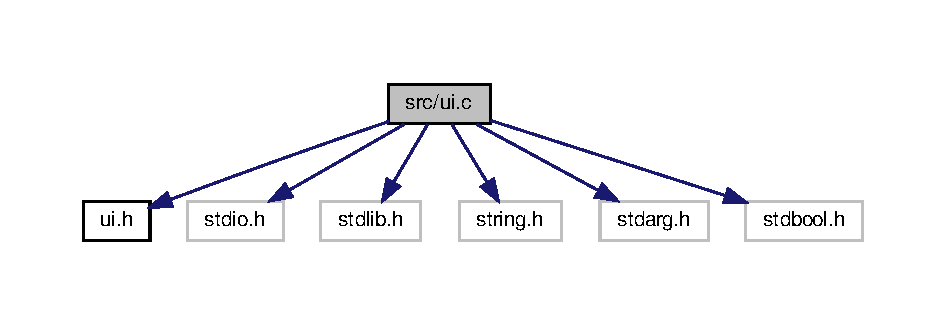
\includegraphics[width=350pt]{ui_8c__incl}
\end{center}
\end{figure}
\subsection*{Data Structures}
\begin{DoxyCompactItemize}
\item 
struct \hyperlink{struct__Ui__pix}{\+\_\+\+Ui\+\_\+pix}
\begin{DoxyCompactList}\small\item\em Basic pixel structure. \end{DoxyCompactList}\item 
struct \hyperlink{struct__Ui__cpix}{\+\_\+\+Ui\+\_\+cpix}
\item 
struct \hyperlink{struct__Ui__box}{\+\_\+\+Ui\+\_\+box}
\begin{DoxyCompactList}\small\item\em Main box structure. \end{DoxyCompactList}\item 
struct \hyperlink{struct__Ui__screen}{\+\_\+\+Ui\+\_\+screen}
\begin{DoxyCompactList}\small\item\em Main UI screen structure. \end{DoxyCompactList}\item 
struct \hyperlink{struct__Ui}{\+\_\+\+Ui}
\begin{DoxyCompactList}\small\item\em Main UI structure. \end{DoxyCompactList}\end{DoxyCompactItemize}
\subsection*{Macros}
\begin{DoxyCompactItemize}
\item 
\mbox{\Hypertarget{ui_8c_ad72dbcf6d0153db1b8d8a58001feed83}\label{ui_8c_ad72dbcf6d0153db1b8d8a58001feed83}} 
\#define {\bfseries D\+E\+B\+UG}
\item 
\mbox{\Hypertarget{ui_8c_ad708dfbbffe55244e42be0875fa9029d}\label{ui_8c_ad708dfbbffe55244e42be0875fa9029d}} 
\#define {\bfseries D\+E\+F\+A\+U\+L\+T\+\_\+\+T\+X\+T\+\_\+\+B\+G\+\_\+\+C\+O\+L\+OR}~\hyperlink{ui_8h_ab87bacfdad76e61b9412d7124be44c1caecc0ff952194921d53813a10bfe2b4d6}{B\+G\+\_\+\+W\+H\+I\+TE}
\item 
\mbox{\Hypertarget{ui_8c_aa3a74dc9689a2b55fcd9f966163390a3}\label{ui_8c_aa3a74dc9689a2b55fcd9f966163390a3}} 
\#define {\bfseries D\+E\+F\+A\+U\+L\+T\+\_\+\+T\+X\+T\+\_\+\+F\+G\+\_\+\+C\+O\+L\+OR}~\hyperlink{ui_8h_ab87bacfdad76e61b9412d7124be44c1ca4d96567df68528c808c8fca495e08098}{F\+G\+\_\+\+B\+L\+A\+CK}
\item 
\mbox{\Hypertarget{ui_8c_a4249ebb1adda7dd451bc03213b87053a}\label{ui_8c_a4249ebb1adda7dd451bc03213b87053a}} 
\#define {\bfseries D\+E\+F\+A\+U\+L\+T\+\_\+\+T\+X\+T\+\_\+\+F\+O\+R\+M\+AT}~\hyperlink{ui_8h_ab4e88c89b3b7ea1735996cc4def22d58a7ec4e09925986b754439a1f94a0d96db}{S\+\_\+\+D\+E\+F\+A\+U\+LT}
\item 
\mbox{\Hypertarget{ui_8c_a5d14091fc31aaec2ac3ecfc410403598}\label{ui_8c_a5d14091fc31aaec2ac3ecfc410403598}} 
\#define {\bfseries D\+E\+F\+A\+U\+L\+T\+\_\+\+B\+O\+X\+\_\+\+B\+G\+\_\+\+C\+O\+L\+OR}~\hyperlink{ui_8h_ab87bacfdad76e61b9412d7124be44c1caecc0ff952194921d53813a10bfe2b4d6}{B\+G\+\_\+\+W\+H\+I\+TE}
\item 
\mbox{\Hypertarget{ui_8c_a1dc97fa1b67c838b5f997b20e8d4b4f9}\label{ui_8c_a1dc97fa1b67c838b5f997b20e8d4b4f9}} 
\#define {\bfseries D\+E\+F\+A\+U\+L\+T\+\_\+\+B\+G\+\_\+\+C\+O\+L\+OR}~\hyperlink{ui_8h_ab87bacfdad76e61b9412d7124be44c1caecc0ff952194921d53813a10bfe2b4d6}{B\+G\+\_\+\+W\+H\+I\+TE}
\item 
\mbox{\Hypertarget{ui_8c_a0a87959b3464403d59d798b987218e4e}\label{ui_8c_a0a87959b3464403d59d798b987218e4e}} 
\#define \hyperlink{ui_8c_a0a87959b3464403d59d798b987218e4e}{U\+I\+\_\+\+T\+A\+B\+\_\+\+S\+I\+ZE}~3
\begin{DoxyCompactList}\small\item\em Tab key size. \end{DoxyCompactList}\item 
\mbox{\Hypertarget{ui_8c_a1be73fb0e5253951bdb7f2a4bd6a1524}\label{ui_8c_a1be73fb0e5253951bdb7f2a4bd6a1524}} 
\#define \hyperlink{ui_8c_a1be73fb0e5253951bdb7f2a4bd6a1524}{U\+I\+\_\+\+M\+A\+X\+\_\+\+B\+O\+X\+ES}~15
\begin{DoxyCompactList}\small\item\em Maximum quantity of boxes per UI. \end{DoxyCompactList}\item 
\mbox{\Hypertarget{ui_8c_a1fb056d53ca550cf384a4dfe0af616af}\label{ui_8c_a1fb056d53ca550cf384a4dfe0af616af}} 
\#define \hyperlink{ui_8c_a1fb056d53ca550cf384a4dfe0af616af}{U\+I\+\_\+\+M\+A\+X\+\_\+\+B\+U\+F\+F\+\_\+\+L\+EN}~500
\begin{DoxyCompactList}\small\item\em Maximum buffer length. \end{DoxyCompactList}\item 
\mbox{\Hypertarget{ui_8c_a0695aa54989d97bfeeb2c65e36a5ad13}\label{ui_8c_a0695aa54989d97bfeeb2c65e36a5ad13}} 
\#define \hyperlink{ui_8c_a0695aa54989d97bfeeb2c65e36a5ad13}{U\+I\+\_\+\+M\+A\+X\+\_\+\+F\+RM}~20
\begin{DoxyCompactList}\small\item\em Maximum number of parameters for formatting. \end{DoxyCompactList}\item 
\mbox{\Hypertarget{ui_8c_aa491d6f223cbad9e34fff4c5e09efd1d}\label{ui_8c_aa491d6f223cbad9e34fff4c5e09efd1d}} 
\#define \hyperlink{ui_8c_aa491d6f223cbad9e34fff4c5e09efd1d}{U\+I\+\_\+\+M\+A\+X\+\_\+\+S\+F\+R\+M\+\_\+\+L\+EN}~100
\begin{DoxyCompactList}\small\item\em Maximum string fromat length. \end{DoxyCompactList}\item 
\mbox{\Hypertarget{ui_8c_aab208380ff579bef5fd8b91fa0c0215a}\label{ui_8c_aab208380ff579bef5fd8b91fa0c0215a}} 
\#define \hyperlink{ui_8c_aab208380ff579bef5fd8b91fa0c0215a}{U\+I\+\_\+\+M\+A\+X\+\_\+\+F\+R\+M\+\_\+\+L\+EN}~( \hyperlink{ui_8c_a0695aa54989d97bfeeb2c65e36a5ad13}{U\+I\+\_\+\+M\+A\+X\+\_\+\+F\+RM} + 2 )
\begin{DoxyCompactList}\small\item\em Maximum length of the format array. \end{DoxyCompactList}\item 
\mbox{\Hypertarget{ui_8c_aeb64a6a8beea1e0e99a8b2ce3bbe170c}\label{ui_8c_aeb64a6a8beea1e0e99a8b2ce3bbe170c}} 
\#define {\bfseries \+\_\+\+\_\+frmidx}(\+\_\+\+\_\+frm)~( \+\_\+\+\_\+frm\mbox{[} \hyperlink{ui_8c_aab208380ff579bef5fd8b91fa0c0215a}{U\+I\+\_\+\+M\+A\+X\+\_\+\+F\+R\+M\+\_\+\+L\+EN} -\/ 2 \mbox{]} ) /$\ast$ get the destination index of the format $\ast$/
\item 
\mbox{\Hypertarget{ui_8c_a9442c04c39b98c383602b108a7aec71c}\label{ui_8c_a9442c04c39b98c383602b108a7aec71c}} 
\#define {\bfseries \+\_\+\+\_\+frmxor}(\+\_\+\+\_\+frm)~( \+\_\+\+\_\+frm\mbox{[} \hyperlink{ui_8c_aab208380ff579bef5fd8b91fa0c0215a}{U\+I\+\_\+\+M\+A\+X\+\_\+\+F\+R\+M\+\_\+\+L\+EN} -\/ 1 \mbox{]} ) /$\ast$ get the checksum of the format $\ast$/
\end{DoxyCompactItemize}
\subsection*{Functions}
\begin{DoxyCompactItemize}
\item 
\hyperlink{struct__Ui__pix}{Ui\+\_\+pix} $\ast$$\ast$ \hyperlink{ui_8c_a698711a3b185d76be3bc27576c01054b}{alloc\+\_\+pixs} (int \+\_\+\+\_\+len)
\begin{DoxyCompactList}\small\item\em Reserves memory to alloc a certain quantity of pixels. \end{DoxyCompactList}\item 
void \hyperlink{ui_8c_afde9d47a49687dc0831376c3f2454259}{kill\+\_\+pixs} (\hyperlink{struct__Ui__pix}{Ui\+\_\+pix} $\ast$$\ast$\+\_\+\+\_\+pixs, int \+\_\+\+\_\+len)
\begin{DoxyCompactList}\small\item\em This function destroys an array of pixels to liberate memory. \end{DoxyCompactList}\item 
\hyperlink{struct__Ui__cpix}{Ui\+\_\+cpix} $\ast$$\ast$ \hyperlink{ui_8c_a299dc91882e1d5f51a7c9f0346f0abdd}{alloc\+\_\+cpixs} (int \+\_\+\+\_\+len)
\begin{DoxyCompactList}\small\item\em Reserves memory to alloc a certain quantity of cache pixels. \end{DoxyCompactList}\item 
void \hyperlink{ui_8c_a6338ee0b6902cc5d197370fb900540dc}{kill\+\_\+cpixs} (\hyperlink{struct__Ui__cpix}{Ui\+\_\+cpix} $\ast$$\ast$\+\_\+\+\_\+pixs, int \+\_\+\+\_\+len)
\begin{DoxyCompactList}\small\item\em This function destroys an array of cache pixels to liberate memory. \end{DoxyCompactList}\item 
bool \hyperlink{ui_8c_a4c6715d14c979c363f6dd1876a2db06a}{ui\+\_\+pix\+\_\+ovf} (int x, int y, int w, int h)
\begin{DoxyCompactList}\small\item\em Checks if a given position ( usually for pixels ) is overflowing the max size. \end{DoxyCompactList}\item 
\hyperlink{struct__Ui__pix}{Ui\+\_\+pix} $\ast$ \hyperlink{ui_8c_abdf66a7ffe3750fb2371e14178d91561}{ui\+\_\+get\+\_\+pix} (\hyperlink{struct__Ui__pix}{Ui\+\_\+pix} $\ast$$\ast$\+\_\+\+\_\+pixs, int x, int y, int w, int h)
\begin{DoxyCompactList}\small\item\em Gets a pixel that is located in a given position. \end{DoxyCompactList}\item 
void \hyperlink{ui_8c_af6c65abe47ab9915826c7490f00becfe}{ui\+\_\+set\+\_\+pix} (\hyperlink{struct__Ui__pix}{Ui\+\_\+pix} $\ast$$\ast$\+\_\+\+\_\+pixs, int x, int y, int w, int h, \hyperlink{struct__Ui__pix}{Ui\+\_\+pix} pix)
\begin{DoxyCompactList}\small\item\em Sets a given pixel in a given position. \end{DoxyCompactList}\item 
\hyperlink{struct__Ui__box}{Ui\+\_\+box} $\ast$ \hyperlink{ui_8c_a007fbe4446d1945531b3b21c06678659}{ui\+\_\+get\+\_\+box\+\_\+by\+\_\+id} (\hyperlink{struct__Ui}{Ui} $\ast$ui, int id)
\begin{DoxyCompactList}\small\item\em Finds a box by it\textquotesingle{}s id (slow) \end{DoxyCompactList}\item 
\hyperlink{struct__Ui__box}{Ui\+\_\+box} $\ast$ \hyperlink{ui_8c_a83fbc61bd07e50156f4526d0b412017f}{ui\+\_\+get\+\_\+box\+\_\+by\+\_\+idx} (\hyperlink{struct__Ui}{Ui} $\ast$ui, int idx)
\begin{DoxyCompactList}\small\item\em Gets a box by it\textquotesingle{}s idx (fast) \end{DoxyCompactList}\item 
void \hyperlink{ui_8c_aa20d570ab281c0262dde9440f9fbc9c3}{ui\+\_\+kill\+\_\+box} (\hyperlink{struct__Ui}{Ui} $\ast$ui, int idx)
\begin{DoxyCompactList}\small\item\em Destroys a given box. \end{DoxyCompactList}\item 
void \hyperlink{ui_8c_aef97744c8290fc4837d2238279d0f4f1}{\+\_\+frm\+\_\+rs} (int $\ast$frm)
\begin{DoxyCompactList}\small\item\em Resets the format. \end{DoxyCompactList}\item 
void \hyperlink{ui_8c_ad9fc8b100e2d6b12926b604c85360c61}{\+\_\+frm\+\_\+cpy} (int $\ast$dest, int $\ast$src)
\begin{DoxyCompactList}\small\item\em Copies source format into destinationformat. \end{DoxyCompactList}\item 
void \hyperlink{ui_8c_a5b9451032a7b28000f768915c526935b}{\+\_\+frm\+\_\+add} (int $\ast$frm, int v)
\begin{DoxyCompactList}\small\item\em Adds a value to a given format. \end{DoxyCompactList}\item 
void \hyperlink{ui_8c_a1968a1e1276abd333bbdfc77338abe9e}{\+\_\+frm} (int $\ast$frm, int n, va\+\_\+list list)
\begin{DoxyCompactList}\small\item\em Adds a list of values into a format array. \end{DoxyCompactList}\item 
void \hyperlink{ui_8c_a91d6818962011df968e8e6fca315a66a}{\+\_\+frm\+\_\+parse} (int $\ast$frm, int $\ast$defrm, const char $\ast$sfrm)
\begin{DoxyCompactList}\small\item\em Parses a given format string into a number format array. \end{DoxyCompactList}\item 
\mbox{\Hypertarget{ui_8c_abb4052814e513471d273eaf1dce5d6fb}\label{ui_8c_abb4052814e513471d273eaf1dce5d6fb}} 
int {\bfseries vsnprintf} (char $\ast$buf, size\+\_\+t size, const char $\ast$fmt, va\+\_\+list list)
\item 
\mbox{\Hypertarget{ui_8c_aed3a44ce00b8d92f93e8a34e7b9dbf54}\label{ui_8c_aed3a44ce00b8d92f93e8a34e7b9dbf54}} 
int {\bfseries snprintf} (char $\ast$buf, size\+\_\+t size, const char $\ast$fmt,...)
\item 
void \hyperlink{ui_8c_a70ca5594ea91504bec5a8a16826f3c23}{ui\+\_\+frm} (\hyperlink{struct__Ui}{Ui} $\ast$ui, int n,...)
\begin{DoxyCompactList}\small\item\em Sets a temporary format of the UI This means that all the text, shapes and other items will use the format that was setted in the last \hyperlink{ui_8h_ad13fb9e90955a66db5a544b87b665ab0}{ui\+\_\+frm()} call. \end{DoxyCompactList}\item 
\mbox{\Hypertarget{ui_8c_ab60af8e54d15c02b3238ddb61a722979}\label{ui_8c_ab60af8e54d15c02b3238ddb61a722979}} 
void {\bfseries ui\+\_\+frms} (\hyperlink{struct__Ui}{Ui} $\ast$ui, const char $\ast$frms,...)
\item 
\hyperlink{struct__Ui}{Ui} $\ast$ \hyperlink{ui_8c_adc8d261a6cf4862dc48958d7fdb5b9c6}{ui\+\_\+init} (int w, int h)
\begin{DoxyCompactList}\small\item\em Initializes UI struct. \end{DoxyCompactList}\item 
void \hyperlink{ui_8c_aa281b74f2ff6f7a1ce8ca79af1371d94}{ui\+\_\+resize} (\hyperlink{struct__Ui}{Ui} $\ast$ui, int w, int h)
\begin{DoxyCompactList}\small\item\em Resizes ui screen. \end{DoxyCompactList}\item 
void \hyperlink{ui_8c_a26dcc63df2a1df20c72a9f8c9eb460d1}{ui\+\_\+destroy} (\hyperlink{struct__Ui}{Ui} $\ast$ui)
\begin{DoxyCompactList}\small\item\em Destroys UI struct. \end{DoxyCompactList}\item 
\mbox{\Hypertarget{ui_8c_aa510252ad42c28b29a27a634e214f9f7}\label{ui_8c_aa510252ad42c28b29a27a634e214f9f7}} 
void {\bfseries ui\+\_\+bg} (\hyperlink{struct__Ui}{Ui} $\ast$ui, const char $\ast$frms,...)
\item 
void \hyperlink{ui_8c_ae33678d6064b4939cd98b2ba7b80357e}{ui\+\_\+rs} (\hyperlink{struct__Ui}{Ui} $\ast$ui)
\begin{DoxyCompactList}\small\item\em Resets the temporary format of the UI to default. \end{DoxyCompactList}\item 
\mbox{\Hypertarget{ui_8c_a9d5dfc09312a1af59fbb102a09c97289}\label{ui_8c_a9d5dfc09312a1af59fbb102a09c97289}} 
void {\bfseries ui\+\_\+box\+\_\+bg} (\hyperlink{struct__Ui}{Ui} $\ast$ui, int idx, const char $\ast$frms,...)
\item 
void \hyperlink{ui_8c_a173b4e0d7bf667e1bf3ae9dadeafae5e}{ui\+\_\+box\+\_\+frm} (\hyperlink{struct__Ui}{Ui} $\ast$ui, int idx, int n,...)
\begin{DoxyCompactList}\small\item\em Sets the default format for the content of the box. \end{DoxyCompactList}\item 
\mbox{\Hypertarget{ui_8c_adf147de26450c9f5e10717a93c6478b6}\label{ui_8c_adf147de26450c9f5e10717a93c6478b6}} 
void {\bfseries ui\+\_\+box\+\_\+frms} (\hyperlink{struct__Ui}{Ui} $\ast$ui, int idx, const char $\ast$frms,...)
\item 
void \hyperlink{ui_8c_a90c0c042767780dd5f4eba555b77c9a9}{ui\+\_\+box\+\_\+repos} (\hyperlink{struct__Ui}{Ui} $\ast$ui, int idx, int x, int y)
\begin{DoxyCompactList}\small\item\em Changes the position of a box. \end{DoxyCompactList}\item 
int \hyperlink{ui_8c_a3aac300e75ad5ae02ae6d371426ca029}{ui\+\_\+box\+\_\+get\+\_\+w} (\hyperlink{struct__Ui}{Ui} $\ast$ui, int idx)
\begin{DoxyCompactList}\small\item\em Get the width of a box (columns) \end{DoxyCompactList}\item 
int \hyperlink{ui_8c_a535313fae3d303f0cb57c04f5d6aee18}{ui\+\_\+box\+\_\+get\+\_\+h} (\hyperlink{struct__Ui}{Ui} $\ast$ui, int idx)
\begin{DoxyCompactList}\small\item\em Get the height of a box (rows) \end{DoxyCompactList}\item 
int \hyperlink{ui_8c_acfefadef83199ecb6fc87386156a1fbb}{ui\+\_\+box\+\_\+get\+\_\+cx} (\hyperlink{struct__Ui}{Ui} $\ast$ui, int idx)
\begin{DoxyCompactList}\small\item\em Get the position of the cursor inside a box (column) \end{DoxyCompactList}\item 
int \hyperlink{ui_8c_a9674fc94b52c30b570a8eccf5f5828cb}{ui\+\_\+box\+\_\+get\+\_\+cy} (\hyperlink{struct__Ui}{Ui} $\ast$ui, int idx)
\begin{DoxyCompactList}\small\item\em Get the position of the cursor inside a box (row) \end{DoxyCompactList}\item 
void \hyperlink{ui_8c_ab8db743aedc69fddc99a3e730396b63d}{ui\+\_\+box\+\_\+set\+\_\+cx\+\_\+off} (\hyperlink{struct__Ui}{Ui} $\ast$ui, int idx, int cx\+\_\+off)
\begin{DoxyCompactList}\small\item\em Sets an offset for the \textquotesingle{}x\textquotesingle{} cursor (column) When the the box is overflowed by it\textquotesingle{}s width the cursor will be resetted to the \textquotesingle{}x\textquotesingle{} position + \textquotesingle{}x\textquotesingle{} offset. \end{DoxyCompactList}\item 
void \hyperlink{ui_8c_a7ee4d3538f3960eec223e1e7d0f0c65a}{ui\+\_\+box\+\_\+set\+\_\+cx\+\_\+top} (\hyperlink{struct__Ui}{Ui} $\ast$ui, int idx, int cx\+\_\+top)
\begin{DoxyCompactList}\small\item\em Sets limit for the \textquotesingle{}x\textquotesingle{} cursor (column) \end{DoxyCompactList}\item 
void \hyperlink{ui_8c_ad4985e811d68055731364dce02e2404d}{ui\+\_\+box\+\_\+get\+\_\+cursor} (\hyperlink{struct__Ui}{Ui} $\ast$ui, int idx, int $\ast$cx, int $\ast$cy)
\begin{DoxyCompactList}\small\item\em Get the position of the cursor inside a box (column \& row) \end{DoxyCompactList}\item 
void \hyperlink{ui_8c_a1d53dad9b00de3c8f2a91738d573d2fb}{ui\+\_\+box\+\_\+resize} (\hyperlink{struct__Ui}{Ui} $\ast$ui, int idx, int w, int h)
\begin{DoxyCompactList}\small\item\em Changes the size of a box. \end{DoxyCompactList}\item 
void \hyperlink{ui_8c_a8064e9aed23d3cd6f94c20d4d70eb8e6}{ui\+\_\+clear\+\_\+box} (\hyperlink{struct__Ui}{Ui} $\ast$ui, int idx)
\begin{DoxyCompactList}\small\item\em Clears the box buffer. \end{DoxyCompactList}\item 
void \hyperlink{ui_8c_af9b58458649ecd779d095f3d102d85c8}{ui\+\_\+clear} (\hyperlink{struct__Ui}{Ui} $\ast$ui)
\begin{DoxyCompactList}\small\item\em Clears all the UI data, including inherit objects like boxes, shapes, ... \end{DoxyCompactList}\item 
void \hyperlink{ui_8c_a3f68193559fa8a9df589042a4609c97f}{ui\+\_\+new\+\_\+box} (\hyperlink{struct__Ui}{Ui} $\ast$ui, int idx, int x, int y, int w, int h)
\begin{DoxyCompactList}\small\item\em Creates a new box. \end{DoxyCompactList}\item 
void \hyperlink{ui_8c_ab1abb40d629ddab0740bc91321abe91f}{ui\+\_\+box\+\_\+seek} (\hyperlink{struct__Ui}{Ui} $\ast$ui, int idx, int x, int y)
\begin{DoxyCompactList}\small\item\em Changes the cursor position of a box. \end{DoxyCompactList}\item 
void \hyperlink{ui_8c_a411b67344c2e5c9b13a4490ee0d930c4}{ui\+\_\+dump\+\_\+box} (\hyperlink{struct__Ui}{Ui} $\ast$ui, int idx)
\begin{DoxyCompactList}\small\item\em This functions dumps all the box data inside the Ui. \end{DoxyCompactList}\item 
void \hyperlink{ui_8c_a17a69a2f4c1c6ee1c7766c314d481ad4}{ui\+\_\+box\+\_\+pad} (\hyperlink{struct__Ui}{Ui} $\ast$ui, int idx, const char $\ast$pad)
\begin{DoxyCompactList}\small\item\em Sets the padding of a box. \end{DoxyCompactList}\item 
\mbox{\Hypertarget{ui_8c_a76dc97022c2c18996c6846b3c7288b6b}\label{ui_8c_a76dc97022c2c18996c6846b3c7288b6b}} 
void {\bfseries ui\+\_\+box\+\_\+put} (\hyperlink{struct__Ui}{Ui} $\ast$ui, int idx, const char $\ast$frmt,...)
\item 
void \hyperlink{ui_8c_abad117bfcc94b8da0e6074977052c708}{ui\+\_\+draw} (F\+I\+LE $\ast$stream, \hyperlink{struct__Ui}{Ui} $\ast$ui)
\begin{DoxyCompactList}\small\item\em Prints all buffered data inside the UI into the stdout. \end{DoxyCompactList}\end{DoxyCompactItemize}


\subsection{Detailed Description}
Ui source code. 

\begin{DoxyAuthor}{Author}
Javier Romera 
\end{DoxyAuthor}
\begin{DoxyCopyright}{Copyright}
G\+NU Public License 
\end{DoxyCopyright}


\subsection{Function Documentation}
\mbox{\Hypertarget{ui_8c_a698711a3b185d76be3bc27576c01054b}\label{ui_8c_a698711a3b185d76be3bc27576c01054b}} 
\index{ui.\+c@{ui.\+c}!alloc\+\_\+pixs@{alloc\+\_\+pixs}}
\index{alloc\+\_\+pixs@{alloc\+\_\+pixs}!ui.\+c@{ui.\+c}}
\subsubsection{\texorpdfstring{alloc\+\_\+pixs()}{alloc\_pixs()}}
{\footnotesize\ttfamily \hyperlink{struct__Ui__pix}{Ui\+\_\+pix} $\ast$$\ast$ alloc\+\_\+pixs (\begin{DoxyParamCaption}\item[{int}]{\+\_\+\+\_\+len }\end{DoxyParamCaption})}



Reserves memory to alloc a certain quantity of pixels. 


\begin{DoxyParams}{Parameters}
{\em \{int\}} & \+\_\+\+\_\+len -\/ The quantity of pixels to be allocted \\
\hline
\end{DoxyParams}

\begin{DoxyRetVals}{Return values}
{\em \{\+Ui\+\_\+pix$\ast$$\ast$\}} & -\/ Returns a pointer which points to other pixels pointers \\
\hline
\end{DoxyRetVals}
\mbox{\Hypertarget{ui_8c_afde9d47a49687dc0831376c3f2454259}\label{ui_8c_afde9d47a49687dc0831376c3f2454259}} 
\index{ui.\+c@{ui.\+c}!kill\+\_\+pixs@{kill\+\_\+pixs}}
\index{kill\+\_\+pixs@{kill\+\_\+pixs}!ui.\+c@{ui.\+c}}
\subsubsection{\texorpdfstring{kill\+\_\+pixs()}{kill\_pixs()}}
{\footnotesize\ttfamily void kill\+\_\+pixs (\begin{DoxyParamCaption}\item[{\hyperlink{struct__Ui__pix}{Ui\+\_\+pix} $\ast$$\ast$}]{\+\_\+\+\_\+pixs,  }\item[{int}]{\+\_\+\+\_\+len }\end{DoxyParamCaption})}



This function destroys an array of pixels to liberate memory. 


\begin{DoxyParams}{Parameters}
{\em \{\+Ui\+\_\+pix$\ast$$\ast$\}} & \+\_\+\+\_\+pixs -\/ Pointer which points to the data \\
\hline
{\em \{int\}} & \+\_\+\+\_\+len -\/ The length of the pixs matrix \\
\hline
\end{DoxyParams}
\mbox{\Hypertarget{ui_8c_a299dc91882e1d5f51a7c9f0346f0abdd}\label{ui_8c_a299dc91882e1d5f51a7c9f0346f0abdd}} 
\index{ui.\+c@{ui.\+c}!alloc\+\_\+cpixs@{alloc\+\_\+cpixs}}
\index{alloc\+\_\+cpixs@{alloc\+\_\+cpixs}!ui.\+c@{ui.\+c}}
\subsubsection{\texorpdfstring{alloc\+\_\+cpixs()}{alloc\_cpixs()}}
{\footnotesize\ttfamily \hyperlink{struct__Ui__cpix}{Ui\+\_\+cpix} $\ast$$\ast$ alloc\+\_\+cpixs (\begin{DoxyParamCaption}\item[{int}]{\+\_\+\+\_\+len }\end{DoxyParamCaption})}



Reserves memory to alloc a certain quantity of cache pixels. 


\begin{DoxyParams}{Parameters}
{\em \{int\}} & \+\_\+\+\_\+len -\/ The quantity of pixels to be allocted \\
\hline
\end{DoxyParams}

\begin{DoxyRetVals}{Return values}
{\em \{\+Ui\+\_\+pix$\ast$$\ast$\}} & -\/ Returns a pointer which points to other pixels pointers \\
\hline
\end{DoxyRetVals}
\mbox{\Hypertarget{ui_8c_a6338ee0b6902cc5d197370fb900540dc}\label{ui_8c_a6338ee0b6902cc5d197370fb900540dc}} 
\index{ui.\+c@{ui.\+c}!kill\+\_\+cpixs@{kill\+\_\+cpixs}}
\index{kill\+\_\+cpixs@{kill\+\_\+cpixs}!ui.\+c@{ui.\+c}}
\subsubsection{\texorpdfstring{kill\+\_\+cpixs()}{kill\_cpixs()}}
{\footnotesize\ttfamily void kill\+\_\+cpixs (\begin{DoxyParamCaption}\item[{\hyperlink{struct__Ui__cpix}{Ui\+\_\+cpix} $\ast$$\ast$}]{\+\_\+\+\_\+pixs,  }\item[{int}]{\+\_\+\+\_\+len }\end{DoxyParamCaption})}



This function destroys an array of cache pixels to liberate memory. 


\begin{DoxyParams}{Parameters}
{\em \{\+Ui\+\_\+pix$\ast$$\ast$\}} & \+\_\+\+\_\+pixs -\/ Pointer which points to the data \\
\hline
{\em \{int\}} & \+\_\+\+\_\+len -\/ The length of the pixs matrix \\
\hline
\end{DoxyParams}
\mbox{\Hypertarget{ui_8c_a4c6715d14c979c363f6dd1876a2db06a}\label{ui_8c_a4c6715d14c979c363f6dd1876a2db06a}} 
\index{ui.\+c@{ui.\+c}!ui\+\_\+pix\+\_\+ovf@{ui\+\_\+pix\+\_\+ovf}}
\index{ui\+\_\+pix\+\_\+ovf@{ui\+\_\+pix\+\_\+ovf}!ui.\+c@{ui.\+c}}
\subsubsection{\texorpdfstring{ui\+\_\+pix\+\_\+ovf()}{ui\_pix\_ovf()}}
{\footnotesize\ttfamily bool ui\+\_\+pix\+\_\+ovf (\begin{DoxyParamCaption}\item[{int}]{x,  }\item[{int}]{y,  }\item[{int}]{w,  }\item[{int}]{h }\end{DoxyParamCaption})}



Checks if a given position ( usually for pixels ) is overflowing the max size. 


\begin{DoxyParams}{Parameters}
{\em \{int\}} & x -\/ Represents the x position ( column of the matrix ) \\
\hline
{\em \{int\}} & y -\/ Represents the y position ( row of the matrix ) \\
\hline
{\em \{int\}} & w -\/ Represents the space width \\
\hline
{\em \{int\}} & h -\/ Represents the space height \\
\hline
\end{DoxyParams}

\begin{DoxyRetVals}{Return values}
{\em \{bool\}} & -\/ Returns a boolean value, false if there is no overflow, else true \\
\hline
\end{DoxyRetVals}
\mbox{\Hypertarget{ui_8c_abdf66a7ffe3750fb2371e14178d91561}\label{ui_8c_abdf66a7ffe3750fb2371e14178d91561}} 
\index{ui.\+c@{ui.\+c}!ui\+\_\+get\+\_\+pix@{ui\+\_\+get\+\_\+pix}}
\index{ui\+\_\+get\+\_\+pix@{ui\+\_\+get\+\_\+pix}!ui.\+c@{ui.\+c}}
\subsubsection{\texorpdfstring{ui\+\_\+get\+\_\+pix()}{ui\_get\_pix()}}
{\footnotesize\ttfamily \hyperlink{struct__Ui__pix}{Ui\+\_\+pix} $\ast$ ui\+\_\+get\+\_\+pix (\begin{DoxyParamCaption}\item[{\hyperlink{struct__Ui__pix}{Ui\+\_\+pix} $\ast$$\ast$}]{\+\_\+\+\_\+pixs,  }\item[{int}]{x,  }\item[{int}]{y,  }\item[{int}]{w,  }\item[{int}]{h }\end{DoxyParamCaption})}



Gets a pixel that is located in a given position. 


\begin{DoxyParams}{Parameters}
{\em \{\+Ui\+\_\+pix$\ast$$\ast$\}} & \+\_\+\+\_\+pixs -\/ the array where the pixel should be located \\
\hline
{\em \{int\}} & x -\/ Represents the x position ( column of the matrix ) \\
\hline
{\em \{int\}} & y -\/ Represents the y position ( row of the matrix ) \\
\hline
{\em \{int\}} & w -\/ Represents the space width \\
\hline
{\em \{int\}} & h -\/ Represents the space height \\
\hline
\end{DoxyParams}

\begin{DoxyRetVals}{Return values}
{\em \{\+Ui\+\_\+pix$\ast$\}} & -\/ Returns a pointer to the found pixel, else returns N\+U\+LL \\
\hline
\end{DoxyRetVals}
\mbox{\Hypertarget{ui_8c_af6c65abe47ab9915826c7490f00becfe}\label{ui_8c_af6c65abe47ab9915826c7490f00becfe}} 
\index{ui.\+c@{ui.\+c}!ui\+\_\+set\+\_\+pix@{ui\+\_\+set\+\_\+pix}}
\index{ui\+\_\+set\+\_\+pix@{ui\+\_\+set\+\_\+pix}!ui.\+c@{ui.\+c}}
\subsubsection{\texorpdfstring{ui\+\_\+set\+\_\+pix()}{ui\_set\_pix()}}
{\footnotesize\ttfamily void ui\+\_\+set\+\_\+pix (\begin{DoxyParamCaption}\item[{\hyperlink{struct__Ui__pix}{Ui\+\_\+pix} $\ast$$\ast$}]{\+\_\+\+\_\+pixs,  }\item[{int}]{x,  }\item[{int}]{y,  }\item[{int}]{w,  }\item[{int}]{h,  }\item[{\hyperlink{struct__Ui__pix}{Ui\+\_\+pix}}]{pix }\end{DoxyParamCaption})}



Sets a given pixel in a given position. 


\begin{DoxyParams}{Parameters}
{\em \{\+Ui\+\_\+pix$\ast$$\ast$\}} & \+\_\+\+\_\+pixs -\/ the array where the pixel should be located \\
\hline
{\em \{int\}} & x -\/ Represents the x position ( column of the matrix ) \\
\hline
{\em \{int\}} & y -\/ Represents the y position ( row of the matrix ) \\
\hline
{\em \{int\}} & w -\/ Represents the space width \\
\hline
{\em \{int\}} & h -\/ Represents the space height \\
\hline
{\em \{\+Ui\+\_\+pix\}} & pix -\/ Struct of the pixel to be setted \\
\hline
\end{DoxyParams}
\mbox{\Hypertarget{ui_8c_a007fbe4446d1945531b3b21c06678659}\label{ui_8c_a007fbe4446d1945531b3b21c06678659}} 
\index{ui.\+c@{ui.\+c}!ui\+\_\+get\+\_\+box\+\_\+by\+\_\+id@{ui\+\_\+get\+\_\+box\+\_\+by\+\_\+id}}
\index{ui\+\_\+get\+\_\+box\+\_\+by\+\_\+id@{ui\+\_\+get\+\_\+box\+\_\+by\+\_\+id}!ui.\+c@{ui.\+c}}
\subsubsection{\texorpdfstring{ui\+\_\+get\+\_\+box\+\_\+by\+\_\+id()}{ui\_get\_box\_by\_id()}}
{\footnotesize\ttfamily \hyperlink{struct__Ui__box}{Ui\+\_\+box} $\ast$ ui\+\_\+get\+\_\+box\+\_\+by\+\_\+id (\begin{DoxyParamCaption}\item[{\hyperlink{struct__Ui}{Ui} $\ast$}]{ui,  }\item[{int}]{id }\end{DoxyParamCaption})}



Finds a box by it\textquotesingle{}s id (slow) 


\begin{DoxyParams}{Parameters}
{\em \{\+Ui$\ast$\}} & ui -\/ UI where the box should be located \\
\hline
{\em \{int\}} & id -\/ The id of the requested box \\
\hline
\end{DoxyParams}

\begin{DoxyRetVals}{Return values}
{\em \{\+Ui\+\_\+box$\ast$\}} & -\/ If the box was found returns a pointer to the requested box, else returns N\+U\+LL \\
\hline
\end{DoxyRetVals}
\mbox{\Hypertarget{ui_8c_a83fbc61bd07e50156f4526d0b412017f}\label{ui_8c_a83fbc61bd07e50156f4526d0b412017f}} 
\index{ui.\+c@{ui.\+c}!ui\+\_\+get\+\_\+box\+\_\+by\+\_\+idx@{ui\+\_\+get\+\_\+box\+\_\+by\+\_\+idx}}
\index{ui\+\_\+get\+\_\+box\+\_\+by\+\_\+idx@{ui\+\_\+get\+\_\+box\+\_\+by\+\_\+idx}!ui.\+c@{ui.\+c}}
\subsubsection{\texorpdfstring{ui\+\_\+get\+\_\+box\+\_\+by\+\_\+idx()}{ui\_get\_box\_by\_idx()}}
{\footnotesize\ttfamily \hyperlink{struct__Ui__box}{Ui\+\_\+box} $\ast$ ui\+\_\+get\+\_\+box\+\_\+by\+\_\+idx (\begin{DoxyParamCaption}\item[{\hyperlink{struct__Ui}{Ui} $\ast$}]{ui,  }\item[{int}]{idx }\end{DoxyParamCaption})}



Gets a box by it\textquotesingle{}s idx (fast) 


\begin{DoxyParams}{Parameters}
{\em \{\+Ui$\ast$\}} & ui -\/ UI where the box should be located \\
\hline
{\em \{int\}} & id -\/ The id of the requested box \\
\hline
\end{DoxyParams}

\begin{DoxyRetVals}{Return values}
{\em \{\+Ui\+\_\+box$\ast$\}} & -\/ The box at the given index (can be N\+U\+LL) \\
\hline
\end{DoxyRetVals}
\mbox{\Hypertarget{ui_8c_aa20d570ab281c0262dde9440f9fbc9c3}\label{ui_8c_aa20d570ab281c0262dde9440f9fbc9c3}} 
\index{ui.\+c@{ui.\+c}!ui\+\_\+kill\+\_\+box@{ui\+\_\+kill\+\_\+box}}
\index{ui\+\_\+kill\+\_\+box@{ui\+\_\+kill\+\_\+box}!ui.\+c@{ui.\+c}}
\subsubsection{\texorpdfstring{ui\+\_\+kill\+\_\+box()}{ui\_kill\_box()}}
{\footnotesize\ttfamily void ui\+\_\+kill\+\_\+box (\begin{DoxyParamCaption}\item[{\hyperlink{struct__Ui}{Ui} $\ast$}]{ui,  }\item[{int}]{idx }\end{DoxyParamCaption})}



Destroys a given box. 


\begin{DoxyParams}{Parameters}
{\em \{\+Ui$\ast$\}} & ui -\/ Ui where the box should be removed \\
\hline
{\em \{int\}} & idx -\/ Box index \\
\hline
\end{DoxyParams}
\mbox{\Hypertarget{ui_8c_aef97744c8290fc4837d2238279d0f4f1}\label{ui_8c_aef97744c8290fc4837d2238279d0f4f1}} 
\index{ui.\+c@{ui.\+c}!\+\_\+frm\+\_\+rs@{\+\_\+frm\+\_\+rs}}
\index{\+\_\+frm\+\_\+rs@{\+\_\+frm\+\_\+rs}!ui.\+c@{ui.\+c}}
\subsubsection{\texorpdfstring{\+\_\+frm\+\_\+rs()}{\_frm\_rs()}}
{\footnotesize\ttfamily void \+\_\+frm\+\_\+rs (\begin{DoxyParamCaption}\item[{int $\ast$}]{frm }\end{DoxyParamCaption})}



Resets the format. 


\begin{DoxyParams}{Parameters}
{\em \{int$\ast$\}} & frm -\/ Format array to be reseted\\
\hline
\end{DoxyParams}
formatting functions \mbox{\Hypertarget{ui_8c_ad9fc8b100e2d6b12926b604c85360c61}\label{ui_8c_ad9fc8b100e2d6b12926b604c85360c61}} 
\index{ui.\+c@{ui.\+c}!\+\_\+frm\+\_\+cpy@{\+\_\+frm\+\_\+cpy}}
\index{\+\_\+frm\+\_\+cpy@{\+\_\+frm\+\_\+cpy}!ui.\+c@{ui.\+c}}
\subsubsection{\texorpdfstring{\+\_\+frm\+\_\+cpy()}{\_frm\_cpy()}}
{\footnotesize\ttfamily void \+\_\+frm\+\_\+cpy (\begin{DoxyParamCaption}\item[{int $\ast$}]{dest,  }\item[{int $\ast$}]{src }\end{DoxyParamCaption})}



Copies source format into destinationformat. 


\begin{DoxyParams}{Parameters}
{\em \{int$\ast$\}} & dest -\/ Format array destination \\
\hline
{\em \{int$\ast$\}} & src -\/ Format array source \\
\hline
\end{DoxyParams}
\mbox{\Hypertarget{ui_8c_a5b9451032a7b28000f768915c526935b}\label{ui_8c_a5b9451032a7b28000f768915c526935b}} 
\index{ui.\+c@{ui.\+c}!\+\_\+frm\+\_\+add@{\+\_\+frm\+\_\+add}}
\index{\+\_\+frm\+\_\+add@{\+\_\+frm\+\_\+add}!ui.\+c@{ui.\+c}}
\subsubsection{\texorpdfstring{\+\_\+frm\+\_\+add()}{\_frm\_add()}}
{\footnotesize\ttfamily void \+\_\+frm\+\_\+add (\begin{DoxyParamCaption}\item[{int $\ast$}]{frm,  }\item[{int}]{v }\end{DoxyParamCaption})}



Adds a value to a given format. 


\begin{DoxyParams}{Parameters}
{\em \{int$\ast$\}} & frm -\/ Format array to be modified \\
\hline
{\em \{int\}} & v -\/ Value to be added \\
\hline
\end{DoxyParams}
\mbox{\Hypertarget{ui_8c_a1968a1e1276abd333bbdfc77338abe9e}\label{ui_8c_a1968a1e1276abd333bbdfc77338abe9e}} 
\index{ui.\+c@{ui.\+c}!\+\_\+frm@{\+\_\+frm}}
\index{\+\_\+frm@{\+\_\+frm}!ui.\+c@{ui.\+c}}
\subsubsection{\texorpdfstring{\+\_\+frm()}{\_frm()}}
{\footnotesize\ttfamily void \+\_\+frm (\begin{DoxyParamCaption}\item[{int $\ast$}]{frm,  }\item[{int}]{n,  }\item[{va\+\_\+list}]{list }\end{DoxyParamCaption})}



Adds a list of values into a format array. 


\begin{DoxyParams}{Parameters}
{\em \{int$\ast$\}} & frm -\/ format array destination \\
\hline
{\em \{int\}} & n -\/ Number of parameters to be added \\
\hline
{\em \{va\+\_\+list\}} & list -\/ List of parameters to be inserted \\
\hline
\end{DoxyParams}
\mbox{\Hypertarget{ui_8c_a91d6818962011df968e8e6fca315a66a}\label{ui_8c_a91d6818962011df968e8e6fca315a66a}} 
\index{ui.\+c@{ui.\+c}!\+\_\+frm\+\_\+parse@{\+\_\+frm\+\_\+parse}}
\index{\+\_\+frm\+\_\+parse@{\+\_\+frm\+\_\+parse}!ui.\+c@{ui.\+c}}
\subsubsection{\texorpdfstring{\+\_\+frm\+\_\+parse()}{\_frm\_parse()}}
{\footnotesize\ttfamily void \+\_\+frm\+\_\+parse (\begin{DoxyParamCaption}\item[{int $\ast$}]{frm,  }\item[{int $\ast$}]{defrm,  }\item[{const char $\ast$}]{sfrm }\end{DoxyParamCaption})}



Parses a given format string into a number format array. 


\begin{DoxyParams}{Parameters}
{\em \{int$\ast$\}} & frm -\/ Format destination \\
\hline
{\em \{int$\ast$\}} & defrm -\/ Default format in case of reset \\
\hline
{\em \{char$\ast$\}} & sfrm -\/ Format string \\
\hline
\end{DoxyParams}
\mbox{\Hypertarget{ui_8c_a70ca5594ea91504bec5a8a16826f3c23}\label{ui_8c_a70ca5594ea91504bec5a8a16826f3c23}} 
\index{ui.\+c@{ui.\+c}!ui\+\_\+frm@{ui\+\_\+frm}}
\index{ui\+\_\+frm@{ui\+\_\+frm}!ui.\+c@{ui.\+c}}
\subsubsection{\texorpdfstring{ui\+\_\+frm()}{ui\_frm()}}
{\footnotesize\ttfamily void ui\+\_\+frm (\begin{DoxyParamCaption}\item[{\hyperlink{struct__Ui}{Ui} $\ast$}]{ui,  }\item[{int}]{n,  }\item[{}]{... }\end{DoxyParamCaption})}



Sets a temporary format of the UI This means that all the text, shapes and other items will use the format that was setted in the last \hyperlink{ui_8h_ad13fb9e90955a66db5a544b87b665ab0}{ui\+\_\+frm()} call. 


\begin{DoxyParams}{Parameters}
{\em \{\+Ui$\ast$\}} & ui -\/ UI to set the temporary parameters \\
\hline
{\em \{int\}} & n -\/ The number of parameters that will be set \\
\hline
{\em \{int\}} & ... -\/ The N parameters to be set, like B\+G\+\_\+\+R\+ED, S\+\_\+\+B\+O\+LD, ... \\
\hline
\end{DoxyParams}
\mbox{\Hypertarget{ui_8c_adc8d261a6cf4862dc48958d7fdb5b9c6}\label{ui_8c_adc8d261a6cf4862dc48958d7fdb5b9c6}} 
\index{ui.\+c@{ui.\+c}!ui\+\_\+init@{ui\+\_\+init}}
\index{ui\+\_\+init@{ui\+\_\+init}!ui.\+c@{ui.\+c}}
\subsubsection{\texorpdfstring{ui\+\_\+init()}{ui\_init()}}
{\footnotesize\ttfamily \hyperlink{struct__Ui}{Ui}$\ast$ ui\+\_\+init (\begin{DoxyParamCaption}\item[{int}]{w,  }\item[{int}]{h }\end{DoxyParamCaption})}



Initializes UI struct. 


\begin{DoxyParams}{Parameters}
{\em \{int\}} & w -\/ The width of the user interface based on chars \\
\hline
{\em \{int\}} & h -\/ The height of the user interface based on chars \\
\hline
\end{DoxyParams}

\begin{DoxyRetVals}{Return values}
{\em \{\+Ui$\ast$\}} & -\/ Returns an UI pointer \\
\hline
\end{DoxyRetVals}
\mbox{\Hypertarget{ui_8c_aa281b74f2ff6f7a1ce8ca79af1371d94}\label{ui_8c_aa281b74f2ff6f7a1ce8ca79af1371d94}} 
\index{ui.\+c@{ui.\+c}!ui\+\_\+resize@{ui\+\_\+resize}}
\index{ui\+\_\+resize@{ui\+\_\+resize}!ui.\+c@{ui.\+c}}
\subsubsection{\texorpdfstring{ui\+\_\+resize()}{ui\_resize()}}
{\footnotesize\ttfamily void ui\+\_\+resize (\begin{DoxyParamCaption}\item[{\hyperlink{struct__Ui}{Ui} $\ast$}]{ui,  }\item[{int}]{w,  }\item[{int}]{h }\end{DoxyParamCaption})}



Resizes ui screen. 


\begin{DoxyParams}{Parameters}
{\em \{\+Ui$\ast$\}} & ui -\/ A pointer to the UI struct \\
\hline
{\em \{int\}} & w -\/ New width (cols) \\
\hline
{\em \{int\}} & h -\/ New height (rows) \\
\hline
\end{DoxyParams}
\mbox{\Hypertarget{ui_8c_a26dcc63df2a1df20c72a9f8c9eb460d1}\label{ui_8c_a26dcc63df2a1df20c72a9f8c9eb460d1}} 
\index{ui.\+c@{ui.\+c}!ui\+\_\+destroy@{ui\+\_\+destroy}}
\index{ui\+\_\+destroy@{ui\+\_\+destroy}!ui.\+c@{ui.\+c}}
\subsubsection{\texorpdfstring{ui\+\_\+destroy()}{ui\_destroy()}}
{\footnotesize\ttfamily void ui\+\_\+destroy (\begin{DoxyParamCaption}\item[{\hyperlink{struct__Ui}{Ui} $\ast$}]{ui }\end{DoxyParamCaption})}



Destroys UI struct. 


\begin{DoxyParams}{Parameters}
{\em \{\+Ui$\ast$\}} & ui -\/ A pointer to the UI struct \\
\hline
\end{DoxyParams}
\mbox{\Hypertarget{ui_8c_ae33678d6064b4939cd98b2ba7b80357e}\label{ui_8c_ae33678d6064b4939cd98b2ba7b80357e}} 
\index{ui.\+c@{ui.\+c}!ui\+\_\+rs@{ui\+\_\+rs}}
\index{ui\+\_\+rs@{ui\+\_\+rs}!ui.\+c@{ui.\+c}}
\subsubsection{\texorpdfstring{ui\+\_\+rs()}{ui\_rs()}}
{\footnotesize\ttfamily void ui\+\_\+rs (\begin{DoxyParamCaption}\item[{\hyperlink{struct__Ui}{Ui} $\ast$}]{ui }\end{DoxyParamCaption})}



Resets the temporary format of the UI to default. 


\begin{DoxyParams}{Parameters}
{\em \{\+Ui$\ast$\}} & ui -\/ the UI where the temporary parameters should be resetted \\
\hline
\end{DoxyParams}
\mbox{\Hypertarget{ui_8c_a173b4e0d7bf667e1bf3ae9dadeafae5e}\label{ui_8c_a173b4e0d7bf667e1bf3ae9dadeafae5e}} 
\index{ui.\+c@{ui.\+c}!ui\+\_\+box\+\_\+frm@{ui\+\_\+box\+\_\+frm}}
\index{ui\+\_\+box\+\_\+frm@{ui\+\_\+box\+\_\+frm}!ui.\+c@{ui.\+c}}
\subsubsection{\texorpdfstring{ui\+\_\+box\+\_\+frm()}{ui\_box\_frm()}}
{\footnotesize\ttfamily void ui\+\_\+box\+\_\+frm (\begin{DoxyParamCaption}\item[{\hyperlink{struct__Ui}{Ui} $\ast$}]{ui,  }\item[{int}]{idx,  }\item[{int}]{n,  }\item[{}]{... }\end{DoxyParamCaption})}



Sets the default format for the content of the box. 


\begin{DoxyParams}{Parameters}
{\em \{\+Ui$\ast$\}} & ui -\/ UI where the box is located \\
\hline
{\em \{int\}} & id -\/ The id of the box \\
\hline
{\em \{int\}} & n -\/ Number of parameters \\
\hline
{\em \{...\}} & -\/ Style parameters \\
\hline
\end{DoxyParams}
\mbox{\Hypertarget{ui_8c_a90c0c042767780dd5f4eba555b77c9a9}\label{ui_8c_a90c0c042767780dd5f4eba555b77c9a9}} 
\index{ui.\+c@{ui.\+c}!ui\+\_\+box\+\_\+repos@{ui\+\_\+box\+\_\+repos}}
\index{ui\+\_\+box\+\_\+repos@{ui\+\_\+box\+\_\+repos}!ui.\+c@{ui.\+c}}
\subsubsection{\texorpdfstring{ui\+\_\+box\+\_\+repos()}{ui\_box\_repos()}}
{\footnotesize\ttfamily void ui\+\_\+box\+\_\+repos (\begin{DoxyParamCaption}\item[{\hyperlink{struct__Ui}{Ui} $\ast$}]{ui,  }\item[{int}]{idx,  }\item[{int}]{x,  }\item[{int}]{y }\end{DoxyParamCaption})}



Changes the position of a box. 


\begin{DoxyParams}{Parameters}
{\em \{\+Ui$\ast$\}} & ui -\/ UI where the box is stored \\
\hline
{\em \{int\}} & idx -\/ The ID with which the box will be referenced \\
\hline
{\em \{int\}} & x -\/ The new x position of the box ( col of the matrix ) \\
\hline
{\em \{int\}} & y -\/ The new y position of the box ( row of the matrix ) \\
\hline
\end{DoxyParams}
\mbox{\Hypertarget{ui_8c_a3aac300e75ad5ae02ae6d371426ca029}\label{ui_8c_a3aac300e75ad5ae02ae6d371426ca029}} 
\index{ui.\+c@{ui.\+c}!ui\+\_\+box\+\_\+get\+\_\+w@{ui\+\_\+box\+\_\+get\+\_\+w}}
\index{ui\+\_\+box\+\_\+get\+\_\+w@{ui\+\_\+box\+\_\+get\+\_\+w}!ui.\+c@{ui.\+c}}
\subsubsection{\texorpdfstring{ui\+\_\+box\+\_\+get\+\_\+w()}{ui\_box\_get\_w()}}
{\footnotesize\ttfamily int ui\+\_\+box\+\_\+get\+\_\+w (\begin{DoxyParamCaption}\item[{\hyperlink{struct__Ui}{Ui} $\ast$}]{ui,  }\item[{int}]{idx }\end{DoxyParamCaption})}



Get the width of a box (columns) 


\begin{DoxyParams}{Parameters}
{\em \{\+Ui$\ast$\}} & ui -\/ UI where the box is located \\
\hline
{\em \{int\}} & idx -\/ box index \\
\hline
\end{DoxyParams}

\begin{DoxyRetVals}{Return values}
{\em returns} & the width of a box (number of columns) \\
\hline
\end{DoxyRetVals}
\mbox{\Hypertarget{ui_8c_a535313fae3d303f0cb57c04f5d6aee18}\label{ui_8c_a535313fae3d303f0cb57c04f5d6aee18}} 
\index{ui.\+c@{ui.\+c}!ui\+\_\+box\+\_\+get\+\_\+h@{ui\+\_\+box\+\_\+get\+\_\+h}}
\index{ui\+\_\+box\+\_\+get\+\_\+h@{ui\+\_\+box\+\_\+get\+\_\+h}!ui.\+c@{ui.\+c}}
\subsubsection{\texorpdfstring{ui\+\_\+box\+\_\+get\+\_\+h()}{ui\_box\_get\_h()}}
{\footnotesize\ttfamily int ui\+\_\+box\+\_\+get\+\_\+h (\begin{DoxyParamCaption}\item[{\hyperlink{struct__Ui}{Ui} $\ast$}]{ui,  }\item[{int}]{idx }\end{DoxyParamCaption})}



Get the height of a box (rows) 


\begin{DoxyParams}{Parameters}
{\em \{\+Ui$\ast$\}} & ui -\/ UI where the box is located \\
\hline
{\em \{int\}} & idx -\/ box index \\
\hline
\end{DoxyParams}

\begin{DoxyRetVals}{Return values}
{\em returns} & the height of a box (number of rows) \\
\hline
\end{DoxyRetVals}
\mbox{\Hypertarget{ui_8c_acfefadef83199ecb6fc87386156a1fbb}\label{ui_8c_acfefadef83199ecb6fc87386156a1fbb}} 
\index{ui.\+c@{ui.\+c}!ui\+\_\+box\+\_\+get\+\_\+cx@{ui\+\_\+box\+\_\+get\+\_\+cx}}
\index{ui\+\_\+box\+\_\+get\+\_\+cx@{ui\+\_\+box\+\_\+get\+\_\+cx}!ui.\+c@{ui.\+c}}
\subsubsection{\texorpdfstring{ui\+\_\+box\+\_\+get\+\_\+cx()}{ui\_box\_get\_cx()}}
{\footnotesize\ttfamily int ui\+\_\+box\+\_\+get\+\_\+cx (\begin{DoxyParamCaption}\item[{\hyperlink{struct__Ui}{Ui} $\ast$}]{ui,  }\item[{int}]{idx }\end{DoxyParamCaption})}



Get the position of the cursor inside a box (column) 


\begin{DoxyParams}{Parameters}
{\em \{\+Ui$\ast$\}} & ui -\/ UI where the box is located \\
\hline
{\em \{int\}} & idx -\/ box index \\
\hline
\end{DoxyParams}

\begin{DoxyRetVals}{Return values}
{\em returns} & the position of the \textquotesingle{}x\textquotesingle{} cursor (column) \\
\hline
\end{DoxyRetVals}
\mbox{\Hypertarget{ui_8c_a9674fc94b52c30b570a8eccf5f5828cb}\label{ui_8c_a9674fc94b52c30b570a8eccf5f5828cb}} 
\index{ui.\+c@{ui.\+c}!ui\+\_\+box\+\_\+get\+\_\+cy@{ui\+\_\+box\+\_\+get\+\_\+cy}}
\index{ui\+\_\+box\+\_\+get\+\_\+cy@{ui\+\_\+box\+\_\+get\+\_\+cy}!ui.\+c@{ui.\+c}}
\subsubsection{\texorpdfstring{ui\+\_\+box\+\_\+get\+\_\+cy()}{ui\_box\_get\_cy()}}
{\footnotesize\ttfamily int ui\+\_\+box\+\_\+get\+\_\+cy (\begin{DoxyParamCaption}\item[{\hyperlink{struct__Ui}{Ui} $\ast$}]{ui,  }\item[{int}]{idx }\end{DoxyParamCaption})}



Get the position of the cursor inside a box (row) 


\begin{DoxyParams}{Parameters}
{\em \{\+Ui$\ast$\}} & ui -\/ UI where the box is located \\
\hline
{\em \{int\}} & idx -\/ box index \\
\hline
\end{DoxyParams}

\begin{DoxyRetVals}{Return values}
{\em returns} & the position of the \textquotesingle{}y\textquotesingle{} cursor (row) \\
\hline
\end{DoxyRetVals}
\mbox{\Hypertarget{ui_8c_ab8db743aedc69fddc99a3e730396b63d}\label{ui_8c_ab8db743aedc69fddc99a3e730396b63d}} 
\index{ui.\+c@{ui.\+c}!ui\+\_\+box\+\_\+set\+\_\+cx\+\_\+off@{ui\+\_\+box\+\_\+set\+\_\+cx\+\_\+off}}
\index{ui\+\_\+box\+\_\+set\+\_\+cx\+\_\+off@{ui\+\_\+box\+\_\+set\+\_\+cx\+\_\+off}!ui.\+c@{ui.\+c}}
\subsubsection{\texorpdfstring{ui\+\_\+box\+\_\+set\+\_\+cx\+\_\+off()}{ui\_box\_set\_cx\_off()}}
{\footnotesize\ttfamily void ui\+\_\+box\+\_\+set\+\_\+cx\+\_\+off (\begin{DoxyParamCaption}\item[{\hyperlink{struct__Ui}{Ui} $\ast$}]{ui,  }\item[{int}]{idx,  }\item[{int}]{cx\+\_\+off }\end{DoxyParamCaption})}



Sets an offset for the \textquotesingle{}x\textquotesingle{} cursor (column) When the the box is overflowed by it\textquotesingle{}s width the cursor will be resetted to the \textquotesingle{}x\textquotesingle{} position + \textquotesingle{}x\textquotesingle{} offset. 


\begin{DoxyParams}{Parameters}
{\em \{\+Ui$\ast$\}} & ui -\/ UI where the box is located \\
\hline
{\em \{int\}} & idx -\/ box index \\
\hline
{\em \{int\}} & cx\+\_\+off -\/ \textquotesingle{}x\textquotesingle{} cursor offset \\
\hline
\end{DoxyParams}
\mbox{\Hypertarget{ui_8c_a7ee4d3538f3960eec223e1e7d0f0c65a}\label{ui_8c_a7ee4d3538f3960eec223e1e7d0f0c65a}} 
\index{ui.\+c@{ui.\+c}!ui\+\_\+box\+\_\+set\+\_\+cx\+\_\+top@{ui\+\_\+box\+\_\+set\+\_\+cx\+\_\+top}}
\index{ui\+\_\+box\+\_\+set\+\_\+cx\+\_\+top@{ui\+\_\+box\+\_\+set\+\_\+cx\+\_\+top}!ui.\+c@{ui.\+c}}
\subsubsection{\texorpdfstring{ui\+\_\+box\+\_\+set\+\_\+cx\+\_\+top()}{ui\_box\_set\_cx\_top()}}
{\footnotesize\ttfamily void ui\+\_\+box\+\_\+set\+\_\+cx\+\_\+top (\begin{DoxyParamCaption}\item[{\hyperlink{struct__Ui}{Ui} $\ast$}]{ui,  }\item[{int}]{idx,  }\item[{int}]{cx\+\_\+top }\end{DoxyParamCaption})}



Sets limit for the \textquotesingle{}x\textquotesingle{} cursor (column) 


\begin{DoxyParams}{Parameters}
{\em \{\+Ui$\ast$\}} & ui -\/ UI where the box is located \\
\hline
{\em \{int\}} & idx -\/ box index \\
\hline
{\em \{int\}} & cx\+\_\+top -\/ \textquotesingle{}x\textquotesingle{} cursor limit \\
\hline
\end{DoxyParams}
\mbox{\Hypertarget{ui_8c_ad4985e811d68055731364dce02e2404d}\label{ui_8c_ad4985e811d68055731364dce02e2404d}} 
\index{ui.\+c@{ui.\+c}!ui\+\_\+box\+\_\+get\+\_\+cursor@{ui\+\_\+box\+\_\+get\+\_\+cursor}}
\index{ui\+\_\+box\+\_\+get\+\_\+cursor@{ui\+\_\+box\+\_\+get\+\_\+cursor}!ui.\+c@{ui.\+c}}
\subsubsection{\texorpdfstring{ui\+\_\+box\+\_\+get\+\_\+cursor()}{ui\_box\_get\_cursor()}}
{\footnotesize\ttfamily void ui\+\_\+box\+\_\+get\+\_\+cursor (\begin{DoxyParamCaption}\item[{\hyperlink{struct__Ui}{Ui} $\ast$}]{ui,  }\item[{int}]{idx,  }\item[{int $\ast$}]{cx,  }\item[{int $\ast$}]{cy }\end{DoxyParamCaption})}



Get the position of the cursor inside a box (column \& row) 


\begin{DoxyParams}{Parameters}
{\em \{\+Ui$\ast$\}} & ui -\/ UI where the box is located \\
\hline
{\em \{int\}} & idx -\/ box index \\
\hline
{\em \{int$\ast$\}} & cx -\/ where the \textquotesingle{}x\textquotesingle{} cursor should be copied \\
\hline
{\em \{int$\ast$\}} & cy -\/ where the \textquotesingle{}y\textquotesingle{} cursor should be copied \\
\hline
\end{DoxyParams}
\mbox{\Hypertarget{ui_8c_a1d53dad9b00de3c8f2a91738d573d2fb}\label{ui_8c_a1d53dad9b00de3c8f2a91738d573d2fb}} 
\index{ui.\+c@{ui.\+c}!ui\+\_\+box\+\_\+resize@{ui\+\_\+box\+\_\+resize}}
\index{ui\+\_\+box\+\_\+resize@{ui\+\_\+box\+\_\+resize}!ui.\+c@{ui.\+c}}
\subsubsection{\texorpdfstring{ui\+\_\+box\+\_\+resize()}{ui\_box\_resize()}}
{\footnotesize\ttfamily void ui\+\_\+box\+\_\+resize (\begin{DoxyParamCaption}\item[{\hyperlink{struct__Ui}{Ui} $\ast$}]{ui,  }\item[{int}]{idx,  }\item[{int}]{w,  }\item[{int}]{h }\end{DoxyParamCaption})}



Changes the size of a box. 


\begin{DoxyParams}{Parameters}
{\em \{\+Ui$\ast$\}} & ui -\/ UI where the box is stored \\
\hline
{\em \{int\}} & idx -\/ The ID with which the box will be referenced \\
\hline
{\em \{int\}} & w -\/ The new width of the box ( number of cols ) \\
\hline
{\em \{int\}} & h -\/ The new height of the box ( number of rows ) \\
\hline
\end{DoxyParams}
\mbox{\Hypertarget{ui_8c_a8064e9aed23d3cd6f94c20d4d70eb8e6}\label{ui_8c_a8064e9aed23d3cd6f94c20d4d70eb8e6}} 
\index{ui.\+c@{ui.\+c}!ui\+\_\+clear\+\_\+box@{ui\+\_\+clear\+\_\+box}}
\index{ui\+\_\+clear\+\_\+box@{ui\+\_\+clear\+\_\+box}!ui.\+c@{ui.\+c}}
\subsubsection{\texorpdfstring{ui\+\_\+clear\+\_\+box()}{ui\_clear\_box()}}
{\footnotesize\ttfamily void ui\+\_\+clear\+\_\+box (\begin{DoxyParamCaption}\item[{\hyperlink{struct__Ui}{Ui} $\ast$}]{ui,  }\item[{int}]{idx }\end{DoxyParamCaption})}



Clears the box buffer. 


\begin{DoxyParams}{Parameters}
{\em \{\+Ui$\ast$\}} & ui -\/ UI where the box is located \\
\hline
{\em \{int\}} & id -\/ The id of the box \\
\hline
\end{DoxyParams}
\mbox{\Hypertarget{ui_8c_af9b58458649ecd779d095f3d102d85c8}\label{ui_8c_af9b58458649ecd779d095f3d102d85c8}} 
\index{ui.\+c@{ui.\+c}!ui\+\_\+clear@{ui\+\_\+clear}}
\index{ui\+\_\+clear@{ui\+\_\+clear}!ui.\+c@{ui.\+c}}
\subsubsection{\texorpdfstring{ui\+\_\+clear()}{ui\_clear()}}
{\footnotesize\ttfamily void ui\+\_\+clear (\begin{DoxyParamCaption}\item[{\hyperlink{struct__Ui}{Ui} $\ast$}]{ui }\end{DoxyParamCaption})}



Clears all the UI data, including inherit objects like boxes, shapes, ... 


\begin{DoxyParams}{Parameters}
{\em \{\+Ui$\ast$\}} & ui -\/ The UI that should be clered \\
\hline
\end{DoxyParams}
\mbox{\Hypertarget{ui_8c_a3f68193559fa8a9df589042a4609c97f}\label{ui_8c_a3f68193559fa8a9df589042a4609c97f}} 
\index{ui.\+c@{ui.\+c}!ui\+\_\+new\+\_\+box@{ui\+\_\+new\+\_\+box}}
\index{ui\+\_\+new\+\_\+box@{ui\+\_\+new\+\_\+box}!ui.\+c@{ui.\+c}}
\subsubsection{\texorpdfstring{ui\+\_\+new\+\_\+box()}{ui\_new\_box()}}
{\footnotesize\ttfamily void ui\+\_\+new\+\_\+box (\begin{DoxyParamCaption}\item[{\hyperlink{struct__Ui}{Ui} $\ast$}]{ui,  }\item[{int}]{idx,  }\item[{int}]{x,  }\item[{int}]{y,  }\item[{int}]{w,  }\item[{int}]{h }\end{DoxyParamCaption})}



Creates a new box. 


\begin{DoxyParams}{Parameters}
{\em \{\+Ui$\ast$\}} & ui -\/ UI where the box should be created \\
\hline
{\em \{int\}} & idx -\/ The ID with which the box will be referenced \\
\hline
{\em \{int\}} & x -\/ The x position of the box ( col of the matrix ) \\
\hline
{\em \{int\}} & y -\/ The y position of the box ( row of the matrix ) \\
\hline
{\em \{int\}} & w -\/ The width of the box ( number of cols ) \\
\hline
{\em \{int\}} & h -\/ The height of the box ( number of rows ) \\
\hline
\end{DoxyParams}
\mbox{\Hypertarget{ui_8c_ab1abb40d629ddab0740bc91321abe91f}\label{ui_8c_ab1abb40d629ddab0740bc91321abe91f}} 
\index{ui.\+c@{ui.\+c}!ui\+\_\+box\+\_\+seek@{ui\+\_\+box\+\_\+seek}}
\index{ui\+\_\+box\+\_\+seek@{ui\+\_\+box\+\_\+seek}!ui.\+c@{ui.\+c}}
\subsubsection{\texorpdfstring{ui\+\_\+box\+\_\+seek()}{ui\_box\_seek()}}
{\footnotesize\ttfamily void ui\+\_\+box\+\_\+seek (\begin{DoxyParamCaption}\item[{\hyperlink{struct__Ui}{Ui} $\ast$}]{ui,  }\item[{int}]{idx,  }\item[{int}]{x,  }\item[{int}]{y }\end{DoxyParamCaption})}



Changes the cursor position of a box. 


\begin{DoxyParams}{Parameters}
{\em \{\+Ui$\ast$\}} & ui -\/ UI where the box is located \\
\hline
{\em \{int\}} & id -\/ The id of the box \\
\hline
{\em \{int\}} & x -\/ Cursor x position ( col matrix ) \\
\hline
{\em \{int\}} & y -\/ Curosr y position ( row matrix ) \\
\hline
\end{DoxyParams}
\mbox{\Hypertarget{ui_8c_a411b67344c2e5c9b13a4490ee0d930c4}\label{ui_8c_a411b67344c2e5c9b13a4490ee0d930c4}} 
\index{ui.\+c@{ui.\+c}!ui\+\_\+dump\+\_\+box@{ui\+\_\+dump\+\_\+box}}
\index{ui\+\_\+dump\+\_\+box@{ui\+\_\+dump\+\_\+box}!ui.\+c@{ui.\+c}}
\subsubsection{\texorpdfstring{ui\+\_\+dump\+\_\+box()}{ui\_dump\_box()}}
{\footnotesize\ttfamily void ui\+\_\+dump\+\_\+box (\begin{DoxyParamCaption}\item[{\hyperlink{struct__Ui}{Ui} $\ast$}]{ui,  }\item[{int}]{idx }\end{DoxyParamCaption})}



This functions dumps all the box data inside the Ui. 


\begin{DoxyParams}{Parameters}
{\em \{\+Ui$\ast$\}} & ui -\/ The ui where data sohuld be dumped \\
\hline
{\em \{int\}} & id -\/ The id of the box to be dumped \\
\hline
\end{DoxyParams}
\mbox{\Hypertarget{ui_8c_a17a69a2f4c1c6ee1c7766c314d481ad4}\label{ui_8c_a17a69a2f4c1c6ee1c7766c314d481ad4}} 
\index{ui.\+c@{ui.\+c}!ui\+\_\+box\+\_\+pad@{ui\+\_\+box\+\_\+pad}}
\index{ui\+\_\+box\+\_\+pad@{ui\+\_\+box\+\_\+pad}!ui.\+c@{ui.\+c}}
\subsubsection{\texorpdfstring{ui\+\_\+box\+\_\+pad()}{ui\_box\_pad()}}
{\footnotesize\ttfamily void ui\+\_\+box\+\_\+pad (\begin{DoxyParamCaption}\item[{\hyperlink{struct__Ui}{Ui} $\ast$}]{ui,  }\item[{int}]{idx,  }\item[{const char $\ast$}]{pad }\end{DoxyParamCaption})}



Sets the padding of a box. 


\begin{DoxyParams}{Parameters}
{\em \{\+Ui$\ast$\}} & ui -\/ UI where the box is located \\
\hline
{\em \{int\}} & id -\/ The id of the box \\
\hline
{\em \{char$\ast$\}} & pad -\/ The padding of the box \char`\"{}$<$top$>$ $<$right$>$ $<$bottom$>$ $<$left$>$\char`\"{} \\
\hline
\end{DoxyParams}
\mbox{\Hypertarget{ui_8c_abad117bfcc94b8da0e6074977052c708}\label{ui_8c_abad117bfcc94b8da0e6074977052c708}} 
\index{ui.\+c@{ui.\+c}!ui\+\_\+draw@{ui\+\_\+draw}}
\index{ui\+\_\+draw@{ui\+\_\+draw}!ui.\+c@{ui.\+c}}
\subsubsection{\texorpdfstring{ui\+\_\+draw()}{ui\_draw()}}
{\footnotesize\ttfamily void ui\+\_\+draw (\begin{DoxyParamCaption}\item[{F\+I\+LE $\ast$}]{stream,  }\item[{\hyperlink{struct__Ui}{Ui} $\ast$}]{ui }\end{DoxyParamCaption})}



Prints all buffered data inside the UI into the stdout. 


\begin{DoxyParams}{Parameters}
{\em \{\+F\+I\+L\+E$\ast$\}} & stream -\/ Buffer destination \\
\hline
{\em \{\+Ui$\ast$\}} & ui -\/ The UI that sueld be printed \\
\hline
\end{DoxyParams}

%--- End generated contents ---

% Index
\backmatter
\newpage
\phantomsection
\clearemptydoublepage
\addcontentsline{toc}{chapter}{Index}
\printindex

\end{document}
